%!TeX program = XeLaTex
%!TEX encoding = UTF-8 Unicode

\documentclass[10pt,twoside]{book}
\XeTeXlinebreaklocale "my_MM"  %Myanmar line and character breaks
\XeTeXinterwordspaceshaping=2

\usepackage[
    paperheight = 10.2in,
    paperwidth = 7.4in,
    right = 0.8in,
    left = 1.45in,
    top = 0.75in,
    bottom = 0.9in,
    heightrounded,
    asymmetric,
    %showframe
]{geometry}
\usepackage[parfill,indent=2em,skip=3pt plus 1pt]{parskip}

\usepackage{fontspec}

\usepackage{bm}

\usepackage{titlesec}
\usepackage{fancyhdr}

\usepackage[dvipsnames,table]{xcolor}
\usepackage{booktabs}
\usepackage{multirow}
\usepackage{array}
\newcommand{\rowsep}{\arrayrulecolor{black!30}\midrule[0.25pt]\arrayrulecolor{black}}
\usepackage{siunitx}

\usepackage{caption}
\usepackage[labelformat=simple]{subcaption}
%\renewcommand\thesubfigure{\alph{subfigure}}

\usepackage[outputdir=out]{minted}
\usepackage{pifont}

%\usemintedstyle{bw}
\setminted[java]{fontfamily=IBMPlexMonoFamily}
\setminted[text]{fontfamily=IBMPlexMonoFamily}
\setminted[python]{fontfamily=IBMPlexMonoFamily}

\AtBeginEnvironment{minted}{\let\special\mintedspecial} 
\def\mintedspecial{\kern0pt\primitive\special}
\makeatletter
\AtBeginEnvironment{minted}{\dontdofcolorbox}
\def\dontdofcolorbox{\renewcommand\fcolorbox[4][]{##4}}
\makeatother

\usepackage{graphicx}
\usepackage{subcaption}
\usepackage{tikz}
\usetikzlibrary{decorations.pathreplacing,calligraphy}
\usepackage{onimage}
\usetikzlibrary{arrows.meta}
\usepackage{adjustbox}
%https://tex.stackexchange.com/questions/9796/how-to-add-todo-notes
\usepackage[textcolor=blue,
    textsize=scriptsize,
    textwidth=17.5mm,
    color=red!25,
    disable]{todonotes}

\definecolor{boxfillcolor}{RGB}{242,242,242}
\definecolor{boxfillcolor2}{RGB}{232,232,232}

%\newcommand{\mintrule}{0.0pt}
%\newcommand{\mintsep}{5pt}
%\newcommand{\mintframe}{lines}
%\newcommand{\xlftmargin}{2pt}
%\definecolor{mintbgcolor}{RGB}{251, 251, 249}
%\definecolor{mintrulecolor}{RGB}{190,190,190}

\newcommand{\mintrule}{0.5pt}
\newcommand{\mintsep}{2pt}
\newcommand{\mintframe}{leftline}
\newcommand{\xlftmargin}{0pt}
\definecolor{mintbgcolor}{RGB}{255, 255, 255}
\definecolor{mintrulecolor}{RGB}{190,190,190}
% control vspace between two minted env
%\AfterEndEnvironment{minted}{\par\vspace{-\baselineskip}}
\newcommand{\betweenminted}[1]{%
  \par\vspace{-\medskipamount}\vspace{-0.5\baselineskip}%
  \vspace{#1}%
}

\usepackage[most]{tcolorbox}
\newtcolorbox{mytcbox}{
    left=3pt,right=3pt,top=3pt,bottom=3pt,
    colframe=gray,
    boxrule=0.4pt,
    colback=boxfillcolor,
    before upper={\parindent0em}
}

\newtcolorbox{mytcboxflt}{
    left=3pt,right=3pt,top=3pt,bottom=3pt,
    float=htb,
    colframe=gray,
    boxrule=0.4pt,
    colback=boxfillcolor,
    before upper={\parindent0em}
}

\newtcbox{\mytcboxinl}[1][boxfillcolor2]{
    on line,
    arc=1.5pt,colback=#1,colframe=#1!50!black,
    before upper={\rule[-3pt]{0pt}{10pt}},
    boxrule=0pt,
    boxsep=0pt,left=1pt,right=1pt,top=1.25pt,bottom=.7pt
}
    
\usepackage{afterpage}
\newcommand\blankpage{%
    \null
    \thispagestyle{empty}%
    \addtocounter{page}{-1}%
    \newpage}
\usepackage{appendix}
\renewcommand\appendixname{နောက်ဆက်တွဲ}
\renewcommand\appendixpagename{နောက်ဆက်တွဲ}

\newcommand{\bropn}{\{}

\defaultfontfeatures[Padauk Book]{}
\setmainfont[
    Path = fonts/,
    UprightFont = PadaukBook-Regular.ttf,
    BoldFont = PadaukBook-Bold.ttf,
    ItalicFont = PadaukBook-Regular.ttf,    
]{Padauk Book}
[Renderer = Graphite, RawFeature = {Tear drop style washwe=True}]

\newfontfamily{\padaukfamily}{Padauk Book}[
    Path = fonts/,
    UprightFont = PadaukBook-Regular.ttf,
    BoldFont = PadaukBook-Bold.ttf,
    ItalicFont = PadaukBook-Regular.ttf,
    Renderer=OpenType]
\DeclareTextFontCommand{\textpadauk}{\padaukfamily}

\newfontfamily{\jetbrainsmonofamily}{JetBrainsMonoNL}[
    Path = fonts/jetbrains_mono/,
    Scale = 0.80,
    UprightFont=*-Regular.ttf,
    ItalicFont=*-Italic.ttf,
    BoldFont=*-Bold.ttf,
    SmallCapsFont=*-Regular.ttf,
    BoldItalicFont=*-BoldItalic.ttf,
    NFSSFamily=JetBrainsMonoFamily]
\DeclareTextFontCommand{\textjetbrainsmono}{\jetbrainsmonofamily}

\newfontfamily{\ibmplexmonofamily}{IBMPlexMono}[
    Path = fonts/ibm_plex_mono/,
    Scale = 0.84,
    UprightFont=*-Text.ttf,
    ItalicFont=*-TextItalic.ttf,
    BoldFont=*-Bold.ttf,
    SmallCapsFont=*-Regular.ttf,
    BoldItalicFont=*-BoldItalic.ttf,
    HyphenChar=None,
    NFSSFamily=IBMPlexMonoFamily]
\DeclareTextFontCommand{\textibmplexmono}{\ibmplexmonofamily}
\newfontfamily{\ibmplexmonofamilya}{IBMPlexMono}[
    Path = fonts/ibm_plex_mono/,
    UprightFont=*-Text.ttf,
    ItalicFont=*-TextItalic.ttf,
    BoldFont=*-SemiBold.ttf,
    SmallCapsFont=*-Regular.ttf,
    BoldItalicFont=*-SemiBoldItalic.ttf]
\DeclareTextFontCommand{\textibmplexmonoa}{\ibmplexmonofamilya}

\newfontfamily{\ibmplexsansfamily}{IBMPlexSans}[
    Path = fonts/ibm_plex_sans/,
    Scale = 1,
    UprightFont=*-Text.ttf,
    ItalicFont=*-TextItalic.ttf,
    BoldFont=*-Bold.ttf,
    SmallCapsFont=*-Regular.ttf,
    BoldItalicFont=*-BoldItalic.ttf,
    HyphenChar=None]
\DeclareTextFontCommand{\textibmplexsans}{\ibmplexsansfamily}

\newfontfamily{\ibmplexseriffamily}{IBMPlexSerif}[
    Path = fonts/ibm_plex_serif/,
    Scale = 1,
    UprightFont=*-Text.ttf,
    ItalicFont=*-TextItalic.ttf,
    BoldFont=*-Bold.ttf,
    SmallCapsFont=*-Regular.ttf,
    BoldItalicFont=*-BoldItalic.ttf,
    HyphenChar=None]
\DeclareTextFontCommand{\textibmplexserif}{\ibmplexseriffamily}

%
\newfontfamily{\latinmodernfamily}{lmroman10}[
    Path = fonts/latin_modern/,
    Extension = .otf,
    UprightFont = *-regular, 
    BoldFont = *-bold,
    ItalicFont = *-italic,
    BoldItalicFont = *-bolditalic,
    SmallCapsFont = lmromancaps10-regular
]
\DeclareTextFontCommand{\textlatinmodern}{\latinmodernfamily}

% downloaded from https://notofonts.github.io/myanmar/ 
\newfontfamily{\notoserifmmfamily}{Noto Serif Myanmar SemiCondensed}[
    Path=fonts/noto_serif_mm/,
    UprightFont=NotoSerifMyanmar-SemiCondensedLight.ttf,
    ItalicFont = NotoSerifMyanmar-SemiCondensedLight.ttf,
    BoldItalicFont = NotoSerifMyanmar-SemiCondensedMedium.ttf,
    BoldFont=NotoSerifMyanmar-SemiCondensedMedium.ttf, Script=Myanmar]
\DeclareTextFontCommand{\textnotoserifmm}{\notoserifmmfamily}


% for normal paragraphs
\NewDocumentCommand{\fEn}{m}{%
    \textlatinmodern{\addfontfeatures{Scale=MatchLowercase}#1}%
}
\NewDocumentCommand{\fEnBf}{m}{%
    \textlatinmodern{\bfseries\addfontfeatures{Scale=MatchLowercase}{#1}}%
}
\NewDocumentCommand{\fEnEmp}{m}{%
    \textlatinmodern{\itshape #1}%
}

\NewDocumentCommand{\fEnEmpBf}{m}{%
    \textlatinmodern{\bfseries\itshape #1}%
}

% for page numbers on each page
\newfontfamily{\padaukbook}{Padauk Book}[
        Path = fonts/,
        UprightFont = PadaukBook-Regular.ttf,
        BoldFont = PadaukBook-Bold.ttf, Renderer = Graphite, RawFeature = {Tear drop style washwe=True}]
\DeclareTextFontCommand{\textpadaukbook}{\padaukbook}
\NewDocumentCommand{\fPageNo}{m}{%
    \textpadaukbook{%
        \addfontfeatures{Mapping = mmdigit_mapping} #1}%
}
\NewDocumentCommand{\fMM}{m}{%
    \textpadaukbook{%
        \addfontfeatures{Scale=0.9,FakeSlant=0.22} #1}%
}

\NewDocumentCommand{\fMMSm}{m}{%
    \textpadaukbook{%
        \addfontfeatures{Scale=0.94} #1}%
}

%=========================================================================================
% Chapter Title
\NewDocumentCommand{\fChNo}{m}{%
    \begingroup%
    \textnotoserifmm{\addfontfeatures{FakeSlant=0.25, Mapping = mmletter_digit_mapping}#1}%
    \endgroup%
}

\NewDocumentCommand{\fCh}{m}{%
    \begingroup%
    \textnotoserifmm{\addfontfeatures{FakeSlant=0.25}#1}%
    \endgroup%
}

% for section and subsection
\NewDocumentCommand{\fSec}{m}{%
    \begingroup%
    \textnotoserifmm{%
    \addfontfeatures{}%
    #1%
    }%
    \endgroup%
}

\NewDocumentCommand{\fSubSec}{m}{%
    \begingroup%
    \textnotoserifmm{%
    \addfontfeatures{}%
    #1%
    }%
    \endgroup%
}

\NewDocumentCommand{\fSecNo}{m}{%
    \begingroup%
    \textnotoserifmm{%
    \addfontfeatures{Mapping = mmletter_digit_mapping}%
    #1%
    }%
    \endgroup%
}

\NewDocumentCommand{\fCpt}{m}{%
    \begingroup%
    \textnotoserifmm{%
    \addfontfeatures{Scale=0.9}%
    #1%
    }%
    \endgroup%
}

\NewDocumentCommand{\fCptNo}{m}{%
    \begingroup%
    \textnotoserifmm{%
    \addfontfeatures{Mapping = mmletter_digit_mapping,Scale=0.9}%
    #1%
    }%
    \endgroup%
}

\NewDocumentCommand{\fSecCode}{m}{%
    \begingroup%
    \textibmplexmonoa{%
    \addfontfeatures{Scale=1}%
    #1%
    }%
    \endgroup%
}

\NewDocumentCommand{\fChCode}{m}{%
    \begingroup%
    \itshape\textibmplexmonoa{%
    \addfontfeatures{Scale=1}%
    #1%
    }%
    \endgroup%
}

\NewDocumentCommand{\fCode}{m}{%
    \begingroup%
    \textibmplexmono{#1}%
    \endgroup%
}
\NewDocumentCommand{\fCodeBf}{m}{%
    \begingroup%
    \bfseries\textibmplexmono{#1}%
    \endgroup%
}%
\NewDocumentCommand{\fSecCodeBf}{m}{%
    \begingroup%
    \textibmplexmonoa{%
    \bfseries\addfontfeatures{Scale=1}%
    #1%
    }%
    \endgroup%
}
\NewDocumentCommand{\fSubSecCodeBf}{m}{%
    \begingroup%
    \textibmplexmonoa{%
    \bfseries\addfontfeatures{}%
    #1%
    }%
    \endgroup%
}
\NewDocumentCommand{\fCptCodeBf}{m}{%
    \begingroup%
    \textibmplexmonoa{%
    \bfseries\addfontfeatures{Scale=MatchLowercase}%
    #1%
    }%
    \endgroup%
}

\NewDocumentCommand{\fRefNo}{m}{%
    \begingroup%
    \textpadaukbook{%
    \addfontfeatures{Mapping = mmletter_digit_mapping}%
    #1%
    }%
    \endgroup%
}

\NewDocumentCommand{\fOpn}{m}{%
    \begingroup%
    \textpadauk{%
    \addfontfeatures{Renderer=OpenType}%
    #1%
    }%
    \endgroup%
}

% for table head
\NewDocumentCommand{\fTblHead}{m}{%
    \begingroup%
    \bfseries\textnotoserifmm{%
    \addfontfeatures{Scale=MatchLowercase}%
    #1%
    }%
    \endgroup%
}

\NewDocumentCommand{\fCoverTitle}{m}{%
    \begingroup%
    \textibmplexserif{%
    \Huge\addfontfeatures{Color=PythonYellow,Scale=7}%
    #1%
    }%
    \endgroup%
}

\NewDocumentCommand{\fCoverTitleII}{m}{%
    \begingroup%
    \textibmplexsans{%
    \Huge\addfontfeatures{Color=White, Scale=1.4}%
    #1%
    }%
    \endgroup%
}

\NewDocumentCommand{\fEnSnd}{m}{%
    \begingroup%
    \textibmplexserif{%
    \addfontfeatures{Scale=MatchLowercase}%
    #1%
    }%
    \endgroup%
}

\NewDocumentCommand{\fFBTtl}{m}{%
    \begingroup%
    \textibmplexsans{%
    \Huge\addfontfeatures{Color=PythonYellow,Scale=7}%
    #1%
    }%
    \endgroup%
}



\renewcommand{\thechapter}{\arabic{chapter}}
\renewcommand{\chaptername}{အခန်း}

\setlength{\headheight}{14pt}

\titleformat{\chapter}[display]
    {\bfseries\Huge}
    {\fCh{\chaptertitlename}\ \fChNo{\thechapter}} % အခန်း ၁
    {20pt}
    {\Large\fCh} % အခန်းခေါင်းစဉ်

\titleformat{\section}
    {\bfseries\large}
    {\fSecNo\thesection}
    {8pt}
    {\bfseries\fSec}

\titleformat{\subsection}
    {\bfseries}
    {\fSecNo\thesubsection}
    {8pt}
    {\bfseries\fSubSec}

\fancypagestyle{plain}{% plain style is used by pages where new chapter begins
    \fancyhf{}% clear all header and footer fields
    \fancyfoot[C]{\bfseries\fPageNo\thepage}% have page no at the btm for chapter start
}

\fancypagestyle{fancy}{%
    \fancyhf{} % clear all header and footer fields
    \fancyhead[LO,RE]{\bfseries\fPageNo\thepage}
    %\fancyhead[RE]{\leftmark}
    %\fancyhead[LO]{\rightmark}
    \renewcommand{\headrulewidth}{0pt}
    \renewcommand{\footrulewidth}{0pt}
}

\fancypagestyle{fancyfront}{%
    \fancyhf{} % clear all header and footer fields
    \fancyhead[LO,RE]{\bfseries\fEn{\thepage}}
    %\fancyhead[RE]{\leftmark}
    %\fancyhead[LO]{\rightmark}
    \renewcommand{\headrulewidth}{0pt}
    \renewcommand{\footrulewidth}{0pt}
}

\fancypagestyle{plainfront}{% plain style is used by pages where new chapter begins
    \fancyhf{}% clear all header and footer fields
    \fancyfoot[C]{\bfseries\fEn{\thepage}}% have page no at the btm for chapter start
}
\usetikzlibrary{shadows,calc}
% some parameters for customization
\def\shadowshift{1.5pt,-1.5pt}
\def\shadowradius{4pt}
\colorlet{innercolor}{black!50}
\colorlet{outercolor}{gray!5}
% this draws a shadow under a rectangle node
\newcommand\drawshadow[1]{
\begin{pgfonlayer}{shadow}
    \shade[outercolor,inner color=innercolor,outer color=outercolor] ($(#1.south west)+(\shadowshift)+(\shadowradius/2,\shadowradius/2)$) circle (\shadowradius);
    \shade[outercolor,inner color=innercolor,outer color=outercolor] ($(#1.north west)+(\shadowshift)+(\shadowradius/2,-\shadowradius/2)$) circle (\shadowradius);
    \shade[outercolor,inner color=innercolor,outer color=outercolor] ($(#1.south east)+(\shadowshift)+(-\shadowradius/2,\shadowradius/2)$) circle (\shadowradius);
    \shade[outercolor,inner color=innercolor,outer color=outercolor] ($(#1.north east)+(\shadowshift)+(-\shadowradius/2,-\shadowradius/2)$) circle (\shadowradius);
    \shade[top color=innercolor,bottom color=outercolor] ($(#1.south west)+(\shadowshift)+(\shadowradius/2,-\shadowradius/2)$) rectangle ($(#1.south east)+(\shadowshift)+(-\shadowradius/2,\shadowradius/2)$);
    \shade[left color=innercolor,right color=outercolor] ($(#1.south east)+(\shadowshift)+(-\shadowradius/2,\shadowradius/2)$) rectangle ($(#1.north east)+(\shadowshift)+(\shadowradius/2,-\shadowradius/2)$);
    \shade[bottom color=innercolor,top color=outercolor] ($(#1.north west)+(\shadowshift)+(\shadowradius/2,-\shadowradius/2)$) rectangle ($(#1.north east)+(\shadowshift)+(-\shadowradius/2,\shadowradius/2)$);
    \shade[outercolor,right color=innercolor,left color=outercolor] ($(#1.south west)+(\shadowshift)+(-\shadowradius/2,\shadowradius/2)$) rectangle ($(#1.north west)+(\shadowshift)+(\shadowradius/2,-\shadowradius/2)$);
    \shade[outercolor,right color=innercolor,left color=innercolor] ($(#1.north west)+(-\shadowradius/12,\shadowradius/12)$) rectangle ($(#1.south east)+(\shadowradius/12,-\shadowradius/12)$);%Frame
    \filldraw ($(#1.south west)+(\shadowshift)+(\shadowradius/2,\shadowradius/2)$) rectangle ($(#1.north east)+(\shadowshift)-(\shadowradius/2,\shadowradius/2)$);
\end{pgfonlayer}
}
% create a shadow layer, so that we don't need to worry about overdrawing other things
\pgfdeclarelayer{shadow} 
\pgfsetlayers{shadow,main}
% Define image shadow command
\newcommand\shadowimage[2][]{%
\begin{tikzpicture}
\node[anchor=south west,inner sep=0] (image) at (0,0) {\includegraphics[#1]{#2}};
\drawshadow{image}
\end{tikzpicture}}
\renewcommand{\figurename}{ပုံ}
\renewcommand{\tablename}{တေဘဲလ်}
\DeclareCaptionFont{cptfont}{\notoserifmmfamily\addfontfeatures{Scale=0.9}}


% Separator style using colon, dash, etc
% to get "Figure (1):", "Figure(1) - Some caption" etc
\DeclareCaptionLabelSeparator{cptSep}{\quad}

% to get "Figure (1)", "Figure [1]", etc, set to labelformat below
% #1 is Figure, #2 is the figure number 1.1, 1,2, etc
\DeclareCaptionLabelFormat{cptFmt}
    {{\bfseries\fCpt{#1}} {\bfseries\fCptNo{#2}}}

\DeclareCaptionLabelFormat{subCptFmt}
    {{\bfseries\fCptNo{(#2)}}}


\captionsetup[figure]
{
    labelformat=cptFmt,
    singlelinecheck=false,
    margin=0pt,
    justification=raggedright,
    labelsep=cptSep,
    %font={cptfont,bf} % both
    %labelfont={cptfont, bf}, % affect label num and sep 
    textfont={cptfont, bf} % affect only caption title   
}

\captionsetup[subfigure]
{
    labelformat=subCptFmt,
    singlelinecheck=false,
    margin=0pt,
    justification=raggedright,
    labelsep=cptSep,
    %font={cptfont,bf} % both
    %labelfont={cptfont, bf}, % affect label num and sep 
    textfont={cptfont, bf} % affect only caption title   
}

\captionsetup[table]
{
    labelformat=cptFmt,
    singlelinecheck=false,
    margin=0pt,
    justification=raggedright,
    labelsep=cptSep,
    %font={cptfont,bf} % both
    %labelfont={cptfont, bf}, % affect label num and sep 
    textfont={cptfont, bf} % affect only caption title   
}
%\renewcommand{\labelitemi}{\normalfont\ding{239}}
%\renewcommand{\labelitemi}{\color{myItmiColor}\RIGHTarrow}
\let\oldding\ding% Store old \ding in \oldding
\renewcommand{\ding}[2][1]{\scalebox{#1}{\oldding{#2}}}% Scale \oldding via optional argument
\renewcommand{\labelitemi}{\ding[0.6]{110}}

\renewcommand{\labelitemii}{\ding[0.85]{229}}
\renewcommand{\labelitemiii}{\ding[0.85]{229}}
%\renewcommand{\labelitemiii}{\tiny\ding{110}}
\renewcommand{\labelitemiv}{\tiny\ding{110}}



\begin{document}
\pagestyle{empty}
\definecolor{PythonBlue}{RGB}{67, 110, 155}
\definecolor{PythonYellow}{RGB}{250, 224, 117}

\begin{tikzpicture}[remember picture,overlay] 

\node[rectangle,
    draw=PythonBlue,
    text = White,
    fill = PythonBlue, 
    minimum width = 7.4in, 
    minimum height = 10.2in, anchor=west]
    at (current page.west) 
    {};  
\node[left, black, anchor=north west] at (-3, 1)
    {\fCoverTitleII{Begin Modern Programming}};
\node[left, black, anchor=north west] at (-3, -1)
    {\fCoverTitleII{with}};
\node[left, black, rotate=90] at (11, -1)
    {\fCoverTitle{Python}};
\node[left, black, anchor=west] at (-3,-22)
    {\fCoverTitleII{Pyi Soe}};
\end{tikzpicture}
%\pagestyle{empty}
\definecolor{PythonBlue}{RGB}{67, 110, 155}
\definecolor{PythonYellow}{RGB}{250, 224, 117}

\begin{tikzpicture}[remember picture,overlay] 

\node[rectangle,
    draw=PythonBlue,
    text = White,
    fill = PythonBlue, 
    minimum width = 7.4in, 
    minimum height = 10.2in, anchor=west]
    at (current page.west) 
    {};  

\node[left, black, rotate=90] at (5.5, -1)
    {\fFBTtl{MP\textit{w}P}};

\end{tikzpicture}
%\pagestyle{empty}
\definecolor{PythonBlue}{RGB}{67, 110, 155}
\definecolor{PythonYellow}{RGB}{250, 224, 117}

\begin{tikzpicture}[remember picture,overlay] 

\node[rectangle,
    draw=PythonBlue,
    text = White,
    fill = PythonBlue, 
    minimum width = 7.4in, 
    minimum height = 10.2in, anchor=west]
    at (current page.west) 
    {};  

\node[left, black, rotate=90] at (0, -1)  
    {\fCoverTitleII{Begin Modern Programming with}};
\node[left, black, rotate=90] at (4, 2)
    {\fFBTtl{Python}};

\end{tikzpicture}
\pagestyle{fancy}
\pagenumbering{arabic}

\chapter{စက်ရုပ်ကားရဲလ်ဖြင့် ပရိုဂရမ်းမင်းမိတ်ဆက်} \label{ch:ch01}
ကွန်ပျူတာတွေဟာ သက်မဲ့ စက်ပစ္စည်းတွေပါပဲ။ ကားတို့၊ လေယာဉ်တို့နဲ့ မတူတာက ကွန်ပျူတာတွေဟာ စက်ချည်းသက်သက် ဘာအစွမ်းမှ မယ်မယ်ရရ မရှိဘူး။ ဒါပေမဲ့ ဆောင်ရွက်လိုတဲ့ ကိစ္စအဝဝအတွက် ပရိုဂရမ်အမျိုးမျိုး ထည့်ပေးလိုက်တဲ့အခါမှာ သူ့ရဲ့အစွမ်းက အတိုင်းအဆမဲ့ပဲ။ နေရာမျိုးစုံ၊ နယ်ပါယ်မျိုးစုံမှာ အကူအညီပေးနိုင်တဲ့ စွယ်စုံသုံး ပစ္စည်းတစ်ခုဖြစ်သွားတယ်။ ဂီတသံစဉ်တွေကို ဖွင့်ပေးနိုင်သလို အသံလည်းသွင်းပေးနိုင်တယ်။ ရုပ်ရှင်တည်းဖြတ် လုပ်ချင်တာလား။ ပြဿနာမရှိဘူး၊ ကူညီပေးနိုင်တယ်။ နျူကလီး\allowbreak ယား ဓါတ်ပေါင်းဖိုတွေကို စီမံနိုင်သလို မောင်းသူမဲ့ ဒုံးပျံတွေကိုလည်း ပဲ့ထိန်းပေးနိုင်တယ်။ 

ကျွန်တော်တို့တွေ နိစ္စဓူဝ အသုံးပြုနေကြတဲ့ ကား၊ စမတ်ဖုန်း၊ လက်ပါတ်နာရီ၊ မိုက်ခရိုဝေဖ့်မီးဖို၊ အဝတ်လျှော်စက် စတဲ့ စက်ပစ္စည်း အမျိုးမျိုးဟာလည်း ကွန်ပျူတာတွေနဲ့ မကင်းပြန်ပါဘူး။ “ကွန်ပျူတာနည်းပညာ အကူအညီမပါတဲ့ ခေတ်မီဆန်းသစ်တီထွင်မှုဆိုတာ မရှိဘူး” လို့ ဆိုနိုင်ပါတယ်။

တစ်ချက်တစ်ချက် ရိုက်ခတ်လိုက်တဲ့ ကွန်ပျူတာနည်းပညာ လှိုင်းလုံးကြီးတွေဟာ ကမ္ဘာတစ်ဝှမ်းလုံး ပုံစံပြောင်းသွားလောက်အောင် အဟုန်ပြင်းထန်လှတယ်။ ဘီလီယံနဲ့ချီတဲ့ လူတွေ ဆိုရှယ်မီဒီယာတွေပေါ်ကနေ ရုပ်သံတွေနဲ့ ချိတ်ဆက်ပြောဆိုဆက်သွယ်လို့ ရစေတာဟာလည်း ကွန်ပျူတာစနစ်တွေပါပဲ။ \fEn{Artificial Intelligence (AI)} နည်းပညာကြောင့် သက်ရှိတွေမှာပဲတွေ့ရတဲ့ ညာဏ်ရည်မျိုးကို ကွန်ပျူတာတွေမှာလည်း တွေ့လာရပါပြီ။ သင်္ချာပုစ္ဆာတွေ ဖြေရှင်းခြင်း၊ စစ်တုရင်ထိုးခြင်း စတဲ့ကိစ္စမျိုးတွေအပြင် ပန်းချီဆွဲခြင်း၊ ကဗျာရေးစပ်ခြင်း၊ သီချင်းရေးဖွဲ့ခြင်း ကဲ့သို့ အနုပညာဖန်တီးမှုတွေကိုပါ \fEn{AI} က လုပ်ဆောင်ပေးနိုင်ပါတယ်။ နှစ်ဆယ့်တစ်ရာစုရဲ့ အထူးခြားဆုံး \fEn{AI} နည်းပညာလှိုင်းဟာ အရှိန်အဟုန်ပြင်းပြင်း ရိုတ်ခတ်ဖို့ အားယူစ ပြုနေပါပြီ။

‘ကွန်ပျူတာ’ လို့ပြောတဲ့အခါ စက်ပစ္စည်းသက်သက် မဟုတ်ဘဲ ကွန်ပျူတာမှတ်ညာဏ်ထဲက ပရိုဂရမ်တွေလည်း ပါဝင်တယ်ဆိုတာ သတိချပ်ရပါမယ်။ ကွန်ပျူတာတွေ တစ်စုံတစ်ရာ စွမ်းဆောင်နိုင်စေတဲ့  ပရိုဂရမ်တွေ ရေးတဲ့အလုပ်ကို ပရိုဂရမ်းမင်း\fEn{(Programming)} လို့ခေါ်တယ်။

\section{စက်ရုပ် ကားရဲလ်}
% ====================
ပရိုဂရမ်းမင်းဆိုတာ ဘယ်လိုမျိုးလဲ သဘောပေါက်အောင် စာတွေတစ်သီကြီးရေး ရှင်းပြတာထက် ပရိုဂရမ်လေးတွေ လက်တွေ့ ရေးကြည့်လိုက်တာ ပိုပြီးထိရောက်ပါတယ်။ ဒါကြောင့် စက်ရုပ်ကားရဲလ်ကို ပရိုဂရမ်လေးတွေရေးပြီး အလုပ်တွေခိုင်းကြည့်ကြမယ်။ ပုံ (\fRefNo{\ref{fig:meet_karel_1}}) မှာ တွေ့ရတာက ကားရဲလ် ရောက်ရှိနေတဲ့ နမူနာ ကမ္ဘာတစ်ခုပါ။ မီးခိုးရောင် မှန်ကူကွက်ပုံလေးကို ဘိပါ \fEn{(beeper)} လို့ ခေါ်တယ်။ အဲဒီဘိပါကို မြှားပြထားတဲ့ နေရာကို ရွှေ့ခိုင်းချင်တယ်။ မျဉ်းမည်းအထူတွေက နံရံတွေပါ။
%
\begin{figure}[htb!]
\begin{tikzonimage}[width=4in]{images/ch_a_programming_with_karel/meet_karel.jpg} %, tsx/show help lines]
    \draw[-{Latex[length=3mm]}] (0.7 ,0.8)--(0.645, 0.635);
\end{tikzonimage}
\caption{စက်ရုပ်လေး ကားရဲလ်}
\label{fig:meet_karel_1}
\end{figure}
%
ကားရဲလ်ကို ကိစ္စတစ်ခု ဆောင်ရွက်စေချင်တဲ့အခါ အခြေခံ ကားရဲလ်ကွန်မန်းတွေကို အသုံးပြုရပါတယ်။ ကွန်မန်းတွေကို နှုတ်နဲ့ပြောပြီး ခိုင်းရတာမဟုတ်ဘဲ ပရိုဂရမ်ရေးပြီး ခိုင်းရတာပါ။ ကားရဲလ်နားလည်တဲ့ ကွန်မန်းတွေကို ကြည့်ကြရအောင်။
%
\subsection*{ကားရဲလ်ကွန်မန်းများ}
% ==========================
မဖြစ်မနေ သိထားရမဲ့ အခြေခံ ကားရဲလ်ကွန်မန်း လေးခုပဲ ရှိတယ်။ \fCode{move}\fEn{,} \fCode{turn\_left}\fEn{,} \fCode{put\_beeper} နဲ့ \fCode{pick\_beeper}\ တို့ဖြစ်တယ်။ အခြား ကားရဲလ်ကွန်မန်း တွေလည်း ရှိပါသေးတယ်။ ဒါပေမဲ့ ကားရဲလ် ပရိုဂရမ်းမင်း စလေ့လာဖို့ ဒီလေးခုနဲ့ပဲ လုံလောက်ပါပြီ။

\fCode{move} ကွန်မန်းက ကားရဲလ်ကို ရှေ့တစ်ကွန်နာကို ရွှေ့ခိုင်းတာ။ ကားရဲလ်ကမ္ဘာထဲမှာ တစ်ခုနဲ့တစ်ခု အကွာအဝေးတူ ခြားထားတဲ့ အတန်းလိုက် အတန်းလိုက် အစက်ကလေးတွေဟာ ကွန်နာ \fEn{(corner)} တွေ ဖြစ်တယ်။ ကမ္ဘာကို မျဉ်းမည်းအထူ နံရံတွေနဲ့ ထောင့်မှန်စတုဂံပုံ ပါတ်လည် ဘောင်ခတ်ထားတယ်။ ကွန်နာတွေကြားမှာလည်း နံရံတွေရှိနိုင်တယ်။ နမူနာကမ္ဘာမှာ ဘေးတိုက် နံပါတ်စဉ် ၄ နဲ့ ၅ ကြား ထောင်လိုက် နံရံတစ်ခု၊ အထက်အောက် နံပါတ်စဉ် ၂ နဲ့ ၃ ကြား အလျားလိုက် နံရံတစ်ခုကို တွေ့ရပါမယ်။ ကွန်နာရှေ့မှာ နံရံကာနေရင် ကားရဲလ်ကို \fCode{move} ခိုင်းလို့မရပါဘူး။ 

\fCode{put\_beeper}\ က ကားရဲလ် လက်ရှိ ရှိနေတဲ့ ကွန်နာမှာ ‘ဘိပါတစ်ခုချ’ ထားခိုင်းတာ၊ \fCode{pick\_beeper}\ က ရပ်နေတဲ့ ကွန်နာမှာ ‘ဘိပါတစ်ခုကောက်’ ခိုင်းတာပါ။ ကွန်နာမှာ ဘိပါရှိနေမှ ကောက်ခိုင်းလို့ရမှာပါ။ မရှိရင် ကောက်ခိုင်းလို့ မရဘူး။ ဘိပါချခိုင်းရင်လည်း ကားရဲလ်မှာ ဘိပါရှိမှ ချခိုင်းလို့ရတယ်။ ကားရဲလ်ကို ဘိပါတွေ လိုသလောက် ဖြည့်ပေးထားတယ်လို့ ယူဆပါ။  \fCode{turn\_left} က ‘ဘယ်လှည့်’ ခိုင်းတာ။ \todo{ကမ္ဘာအသစ်တည်ဆောက်ရင် ဘိပါအရေအတွက် လိုသလိုဖြည့်ထားလို့ရကြောင်း ရှင်းပြဖို့လိုမလား}

\subsection*{ဘိပါကို ဘယ်လိုရွှေ့ခိုင်းမလဲ}
% ================================
ပုံ (\fRefNo{\ref{fig:meet_karel_1}}) အနေအထားကနေ ရှေ့ကို သုံးနေရာရွှေ့၊ ဘိပါကောက်၊ ဘယ်ဘက်လှည့်၊ အပေါ် နှစ်နေရာရွှေ့၊ ညာဘက်လှည့်၊ ရှေ့တစ်နေရာထပ်ရွှေ့ပြီး ဘိပါချထားခိုင်းလိုက်ရင် အလုပ်ပြီးသွားပါပြီ။

ကားရဲလ်ကို ညာဘက်လှည့်ခိုင်းဖို့ \fCode{turn\_right} ကွန်မန်း မရှိဘူး။ ဒါပေမဲ့ ဘယ်သုံးခါလှည့်တာဟာ ညာဘက်လှည့်တာနဲ့ တူတူပါပဲ။ ဒါကြောင့် ညာဘက်ချင်တဲ့အခါ ဘယ်သုံးခါလှည့်ခိုင်းလို့ရတယ်။

\section{Meet Karel ပရိုဂရမ်}
ပရိုဂရမ် ရေးတယ်ဆိုတာ ကွန်ပျူတာကို ကိစ္စတစ်ခုခု ဆောက်ရွက်ပေးဖို့ ခိုင်းစေတဲ့  ညွှန်ကြားချက်တွေ ရေးတာပါပဲ။ ဒီလို ညွှန်ကြားချက်တွေကို ပရိုဂရမ်ကုဒ် \fEn{(program code)} လို့ ခေါ်တယ်။ ပရိုဂရမ်ကုဒ်တွေကို ကွန်ပျူတာနားလည်တဲ့ \fEn{programming language} တစ်ခုခုနဲ့ ရေးရတယ်။ ဒီစာအုပ်မှာ အသုံးပြုမဲ့ \fEn{programming language} ကတော့ \fEn{Python} ပါ။ \fEn{Programming language} တစ်မျိုးပဲ ရှိတာမဟုတ်ပါဘူး။ ရာနဲ့ချီပြီး ရှိတာပါ။ လူ့ဘာသာစကားတွေ အမျိုးမျိုးရှိသလိုပဲပေါ့။ \fEn{Python} ဟာ ဒီလို ရာနဲ့ချီတဲ့ထဲက လက်ရှိအသုံးအများဆုံး ထိပ်ဆုံးဆယ်ခု ထဲမှာ ပါဝင်တယ်။ \fEn{Python} နဲ့ ဘိပါရွှေ့ခိုင်းတဲ့ ပရိုဂရမ်ကို လေ့လာကြည့်ရအောင်။ ကားရဲလ်နဲ့ ပထမဆုံး မိတ်ဆက်ပေးတဲ့ ပရိုဂရမ်မို့လို့ ဒီပရိုဂရမ် နံမည်ကို \fEn{‘Meet Karel’} လို့ ခေါ်ပါမယ်။
%
\setlength{\fboxsep}{0pt}
\begin{minted}[frame=\mintframe, framerule=\mintrule,framesep= \mintsep, xleftmargin=\xlftmargin
    , bgcolor=mintbgcolor,rulecolor=mintrulecolor
    , python3=true,escapeinside=ßß]{python}
# File: meet_karel.py
# About: This is
from stanfordkarel import *


def main():
    """Karel code goes here!"""
    move()
    move()
    move()
    pick_beeper()
    turn_left()
    move()
    move()

    turn_left()
    turn_left()
    turn_left()

    move()
    put_beeper()
# End of main

if __name__ == "__main__":
    run_karel_program("meet_karel")

\end{minted}
%

ဒါဟာ \fEn{‘Meet Karel’} ပရိုဂရမ်အတွက် \fEn{Python} နဲ့ရေးထားတဲ့ ပရိုဂရမ်ကုဒ် တွေဖြစ်ပါတယ်။ ‘\fEn{Python} ကုဒ်’ လို့ အတိုချုံးပဲ ပြောတာများတယ်။ \fEn{Python} ‘စာ/စကား’ မတတ်ရင် ဒီ ‘\fEn{Python} ကုဒ်’ တွေကိုလည်း နားလည်မှာ မဟုတ်ဘူး။ ဒီတော့ \fEn{Python} ‘စာ/စကား’ အခြေခံက စပြီး လေ့လာဖို့ လိုပါမယ်။
\todo{စာ ကို footnote ထည့်ရန်}

\subsection*{ကွန်းမန့် (Comment)}
ပထမဆုံး \fCode{\textit{\#}} သင်္ကေတနဲ့ စတဲ့ စာကြောင်းတွေက ကွန်းမန့်တွေပါ။ ကွန်းမန့်တွေက ကွန်ပျူတာ ဆောင်ရွက်ပေးရမဲ့ ညွှန်ကြားချက်တွေ မဟုတ်ဘူး။ ပရိုဂရမ်ကုဒ်နဲ့ ပါတ်သက်ပြီး ကုဒ် ဖတ်ရှူသူ အတွက် မှတ်ချက်ရေးတာ သို့မဟုတ် ရှင်းပြထားတာပါ။ တနည်းအားဖြင့် ဖတ်ရှုသူ (လူ) ပရိုဂရမ်မာအတွက် ရည်ရွယ်တာ။ ကွန်ပျူတာ (စက်) အတွက် ရည်ရွယ်တာ မဟုတ်ဘူး။ ကွန်ပျူတာက ကုဒ်ထဲက ကွန်းမန့်တွေ အားလုံးကို လစ်လျူရှုမှာပါ။ ဒါပေမဲ့ ပရိုဂရမ်ကုဒ်ကို ဖတ်တဲ့လူ နားလည်ဖို့ အထောက်အကူ ဖြစ်စေတဲ့အတွက် ကွန်းမန့်ရေးတာကို ပေါ့ပေါ့တန်တန် အရေးမပါသလို သဘောထားလို့ မရပါဘူး။ မိမိရေးတဲ့ ကုဒ်ကို ရှင်းပြဖို့ လိုအပ်ရင် ကွန်းမန့်ရေးရပါမယ်။ ရေးသင့်တဲ့ နေရာတွေကိုလည်း မကြာခင်တွေ့ရမှာပါ။

\subsection*{\fSubSecCodeBf{import} စတိတ်မန့်}
%
\setlength{\fboxsep}{0pt}
\begin{minted}[frame=\mintframe, framerule=\mintrule,framesep= \mintsep, xleftmargin=\xlftmargin
    , bgcolor=mintbgcolor,rulecolor=mintrulecolor
    , python3=true,escapeinside=ßß]{python}
from stanfordkarel import *
\end{minted}
%
ကတော့ အင်ပို့စတိတ်မန့် ဖြစ်ပါတယ်။ “\fCode{stanfordkarel} လိုက်ဘရီမှ အာလုံးကို ထည့်သွင်းပေးပါ” လို့ တောင်းဆိုတဲ့ အဓိပ္ပါယ်။ \fCode{*} သင်္ကေတကို ‘အားလုံး’ လို့ ယူဆပါ။  \fCode{stanfordkarel} လိုက်ဘရီမှာ ကားရဲလ်ပရိုဂရမ်အတွက် လိုအပ်တာအားလုံး   ပါဝင်တယ်။  ဒီလိုက်ဘရီကို အင်ပို့လုပ်ထားမှ ကားရဲလ်ကွန်မန်းတွေ သုံးလို့ရမှာပါ။ သီးခြား ကားရဲလ်ပရိုဂရမ် တစ်ခုစီတိုင်းအတွက် အင်ပို့လုပ်ရမှာ ဖြစ်တယ်။

\subsection*{လိုက်ဘရီ}
လိုက်ဘရီ \fEn{(\fEnEmpBf{library})} ဆိုတာ ပညာရပ်နယ်ပယ် တစ်ခုအတွက် ရည်ရွယ်ရေးထားတဲ့ ပရိုဂရမ်ကုဒ်တွေပါပဲ။ သင်္ချာအတွက်အချက် လိုက်ဘရီ၊ ဂိမ်းရေးဖို့ လိုက်ဘရီ၊ \fEn{2D/3D} ဂရပ်ဖစ်ဆွဲဖို့ လိုက်ဘရီ၊ အေအိုင်အတွက် လိုက်ဘရီ စသည်ဖြင့် နယ်ပယ်အသီးသီး၊ ကိစ္စရပ်အဖုံဖုံအတွက် သက်ဆိုင်ရာ ကျွမ်းကျင်ပညာရှင်တွေ ထုတ်လုပ်ဖြန့်ချီပေးထားတဲ့ လိုက်ဘရီတွေရှိတယ်။ \fEn{Matrix} အော်ပရေးရှင်းတွေအတွက် \fCode{numpy} ၊ ဂရပ်ဖ်ဆွဲမယ်ဆိုရင် \fCode{matplotlib} စတဲ့ လိုက်ဘရီတွေကို အင်ပို့လုပ် အသုံးပြုနိုင်ပါတယ်။ မေ့ထရစ် $A$ ကို $B$ နဲ့ မြှောက်ရင် ဒီလိုပါ 
%
\setlength{\fboxsep}{0pt}
\begin{minted}[frame=\mintframe, framerule=\mintrule,framesep= \mintsep, xleftmargin=\xlftmargin
    , bgcolor=mintbgcolor,rulecolor=mintrulecolor
    , python3=true,escapeinside=ßß]{python}
from numpy import *

A = array([[1, 1, 2, 2],
           [2, 2, 1, 1],
           [2, 2, 1, 1]])
B = array([[2, 2],
           [2, 2],
           [1, 1],
           [2, 2]])

result = matmul(A, B)

print(result)

\end{minted}
%
ရလဒ် အခုလိုထွက်ပါမယ်။ 
%
\begin{minted}[frame=lines, framerule=0pt]{text}
[[10 10]
 [11 11]
 [11 11]]
\end{minted}
%
ဒါကတော့ ဘားချတ် အတွက် \fCode{numpy} နဲ့ \fCode{matplotlib} လိုက်ဘရီ သုံးထားတာပါ။  
%
\setlength{\fboxsep}{0pt}
\begin{minted}[frame=\mintframe, framerule=\mintrule,framesep= \mintsep, xleftmargin=\xlftmargin
    , bgcolor=mintbgcolor,rulecolor=mintrulecolor
    , python3=true,escapeinside=ßß]{python}
from matplotlib.pyplot import *
from numpy import *

# make data:
x = 0.5 + arange(8)
y = [4.8, 5.5, 3.5, 4.6, 6.5, 6.6, 2.6, 3.0]

# plot
fig, ax = subplots()
bar(x, y, width=1, edgecolor="white", linewidth=0.7)

ax.set(xlim=(0, 8), xticks=arange(1, 8),
       ylim=(0, 8), yticks=arange(1, 8))

show()
\end{minted}
ဘားချတ်ကို ဒီလို ထုတ်ပေးပါတယ်။
%
\begin{figure}[tbh!]
\begin{tikzpicture}
    \node[anchor=south west,inner sep=0] (image) at (0,0)
        {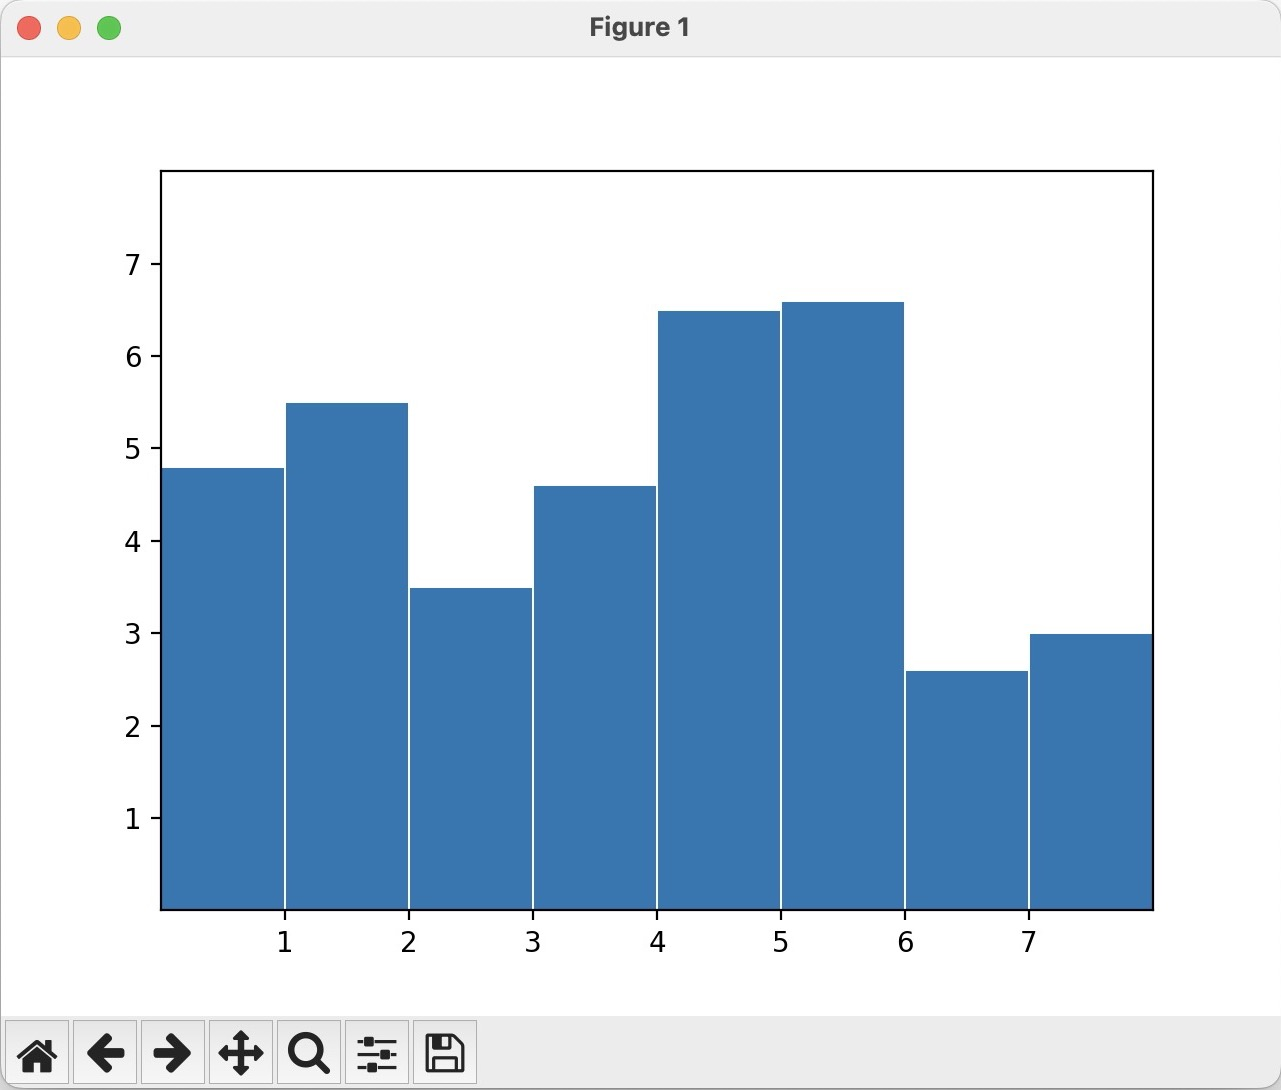
\includegraphics[width=.5\textwidth, trim={2.4mm 2mm 2mm 2mm},clip]{images/ch01/bar.jpg}};
    \drawshadow{image}
\end{tikzpicture}
\caption{} 
\label{fig:}
\end{figure}

လိုက်ဘရီတွေဟာ ပရိုဂရမ်တွေ တည်ဆောက်ရာမှာ အင်မတန်မှ အရေးပါတယ်။ ဖော်ပြထားတဲ့ မေ့ထရစ် နဲ့ ဘားချတ်  ကုဒ်တွေကို (အခုတော့) နားလည်မှာ မဟုတ်သေးဘူးပေါ့။ ဒါပေမဲ့ သက်ဆိုင်ရာ လိုက်ဘရီတွေနဲ့ ဒီလိုကိစ္စတွေကို သိပ်မခက်ခဲဘဲ လုပ်လို့ရနိုင်တယ်ဆိုတာ မြင်မယ် ထင်ပါတယ်။ လိုက်ဘရီတွေသာမရှိရင် ပရိုဂရမ်တွေကို အခုထက် အဆပေါင်းများစွာ အချိန်ပေးပြီး ရှုပ်ရှုပ်ထွေးထွေး ခက်ခက်ခဲခဲ တည်ဆောက်ကြရမှာပါ။ 


\subsection*{တုံကင်၊ စတိတ်မန့်နှင့် ဆင်းတက်စ်}
ဂျန်ပန်စာ၊ ပြင်သစ်စာ စတဲ့ လူ့ဘာသာစကားတွေဟာ  စကားလုံးတွေ ဝါကျတွေနဲ့ ဖွဲ့စည်းထားသလို ပရိုဂရမ်ကုဒ်တွေဟာလည်း စကားလုံးတွေ၊ ဝါကျတွေနဲ့ ဖွဲ့စည်းထားတာပါပဲ။ \fEn{Programming language} တွေမှာ စကားလုံးတွေကို တုံကင် \fEn{(\fEnEmpBf{token})} လို့ခေါ်ပြီး  ဝါကျတွေကိုတော့ စတိတ်မန့် \fEn{(\fEnEmpBf{statement})} လို့ ခေါ်ပါတယ်။ ဝါကျတွေကို စကားလုံးတွေနဲ့ ဖွဲ့စည်းထားသလို စတိတ်မန့်တွေကတော့ တုံကင်တွေနဲ့ ဖွဲ့စည်းထားတာပါ။ စတိတ်မန့် ပုံစံတစ်မျိုးကို တွေခဲ့ပြီးပါပြီ။ အဲဒါကတော့ ရှေ့စာမျက်နှာက အင်ပို့စတိတ်မန့်ပဲ ဖြစ်ပါတယ်။ 

လူ့ဘာသာစကားတွေမှာ ဖွဲ့စည်းတည်ဆောက်ပုံ စထရက်ချာရှိသလို \fEn{programming language} တွေမှာလည်း စထရက်ချာရှိဖို့ လိုအပ်တာပေါ့။  ဖွဲ့စည်းပုံ စထရက်ချာ မှန်/မမှန်ကို သဒ္ဒါစည်းမျဉ်တွေနဲ့ ထိန်းကွပ်ထားတာပါ။ ပရိုဂရမ်ကုဒ် စထရက်ချာ မှန်/မမှန် ထိန်းကွပ်ပေးတဲ့ သဒ္ဒါစည်းမျဉ်တွေကိုတော့ ဆင်းတက်စ် \fEn{(\fEnEmpBf{syntax})} လို့ခေါ်တယ်။

မြန်မာလိုရေးရင် မြန်မာသဒ္ဒါကို လိုက်နာရသလို \fEn{Python} နဲ့ ရေးရင် \fEn{Python} ဆင်းတက်စ်ကို လိုက်နာရမှာပေါ့။ မြန်မာသဒ္ဒါမှားရင် ဖတ်တဲ့သူက သည်းခံနားလည် ပေးပေမဲ့ ဆင်းတက်စ်မှားရင်တော့ \fEn{Python} က လုံးဝ လက်ခံမှာ မဟုတ်ပါဘူး။ ဆင်းတက်စ် စည်းကမ်းတွေဟာ ပိုပြီး တင်းကျပ်တယ်။ လွဲချော်လို့ မရဘူး။ ဆင်းတက်စ်မှားနေတဲ့ ပရိုဂရမ်ကို  \fEn{Python} က \fEn{run} ခွင့် ပြုမှာမဟုတ်ဘဲ အမှားနဲ့သက်ဆိုင်တဲ့ အယ်ရာ\fOpn{မက်ဆေ့ချ်}တွေ ပြပေးမှာပါ။ ဖြစ်လေ့ရှိတဲ့ ဆင်းတက်စ်အမှားတွေကို မကြာခင် တွေ့ရပါမယ်။

\subsection*{Keywords}
\fCode{from}\fEn{,} \fCode{import}\fEn{,} \fCode{def} \fEn{,} \fCode{if} စတာတွေဟာ \fEnEmpBf{keyword} တွေဖြစ်တယ်။ \fEn{Python} ရေးတဲ့အခါ သူ့နေရာနဲ့သူ အဓိပ္ပါယ်ကိုယ်စီနဲ့ အသုံးပြုရတဲ့ စကားလုံးတွေဖြစ်တယ်။ \fCode{from} နဲ့ \fCode{import} ကို လိုက်ဘရီ အင်ပို့လုပ်ဖို့ သုံးတယ်။ \fCode{def} ကို ဖန်ရှင် သတ်မှတ်တဲ့အခါ သုံးတယ်။ \fEn{Python} က သတ်မှတ်ထားတဲ့ နေရာတွေကလွဲလို့ အခြားကိစ္စတွေအတွက် \fEn{keyword} တွေကို အသုံးပြုလို့ မရပါဘူး။ ဒါကြောင့်  \fEn{keyword} တွေကို \fEn{reserved word} လို့လည်း ခေါ်တယ်။ 

\subsection*{\fSubSecCodeBf{main} ဖန်ရှင်}
\fEn{‘Meet Karel’} ပရိုဂရမ် အင်ပို့စတိတ်မန့် အပြီးမှာ တွေ့ရတာကတော့ \fCode{main} ဖန်ရှင်သတ်မှတ်ချက်ပါ။ ကြည့်ရအဆင်ပြေအောင် သူ့ချည်းသီးသန့် တစ်ဖြတ် ပြန်ပြပေးထားပါတယ်။
%
\setlength{\fboxsep}{0pt}
\begin{minted}[frame=\mintframe, framerule=\mintrule,framesep= \mintsep, xleftmargin=\xlftmargin
    , bgcolor=mintbgcolor,rulecolor=mintrulecolor
    , python3=true,escapeinside=ßß]{python}
def main():
    """Karel code goes here!"""
    move()
    move()
    move()
    pick_beeper()
    turn_left()
    move()
    move()

    turn_left()
    turn_left()
    turn_left()

    move()
    put_beeper()
# End of main
\end{minted}

\begin{mytcbox}
ဖန်ရှင် \fEn{(\fEnEmpBf{function})} ဆိုတာ ကိစ္စတစ်ခု လုပ်ဆောင်ပေးဖို့အတွက် ယူနစ်တစ်ခုအနေနဲ့ ဖွဲ့စည်းထားတဲ့ ပရိုဂရမ်ကုဒ် အစုအဝေးတစ်ခုပါပဲ။ ဖန်ရှင်ကို အသုံးပြုတဲ့အခါ ၎င်းရဲ့ လုပ်ငန်းတာဝန်အတိုင်း ဖန်ရှင်က လုပ်ဆောင်ပေးမှာ ဖြစ်တယ်။ ဖန်ရှင်အသုံးပြုတာကို ‘ဖန်ရှင်ကောလ်’  \fEn{(\textit{function call})} လုပ်တာလို့ ပြောတယ်။
\end{mytcbox}
%
\fCode{main} ဖန်ရှင်သတ်မှတ်ချက်ကို အပိုင်းနှစ်ပိုင်းခွဲ ကြည့်နိုင်တယ်။ ပထမတစ်ပိုင်း
%
\setlength{\fboxsep}{0pt}
\begin{minted}[frame=\mintframe, framerule=\mintrule,framesep= \mintsep, xleftmargin=\xlftmargin
    , bgcolor=mintbgcolor,rulecolor=mintrulecolor
    , python3=true,escapeinside=ßß]{python}
def main():
\end{minted}
%
ကို ဖန်ရှင်ခေါင်းစီး \fEn{(function header)} လို့ခေါ်တယ်။ ဖန်ရှင်ခေါင်းစီးမှာ ဖန်ရှင်နံမည်နဲ့ ဖန်ရှင်ပါရာမီတာတွေကို ဝိုက်ကွင်းထဲမှာ သတ်မှတ်ပေးရပြီး ကော်လံ \mytcboxinl{\fCode{:}} နဲ့ အဆုံးသတ်တယ်။ ဥပမာ \fCode{x}\fEn{,} \fCode{y} ပါရာမီတာ နဲ့  \fCode{myfun} ဖန်ရှင် အတွက် 
%
\setlength{\fboxsep}{0pt}
\begin{minted}[frame=\mintframe, framerule=\mintrule,framesep= \mintsep, xleftmargin=\xlftmargin
    , bgcolor=mintbgcolor,rulecolor=mintrulecolor
    , python3=true,escapeinside=ßß]{python}
def myfun(x, y):
\end{minted}
ပါရာမီတာမပါရင်လည်း ဝိုက်ကွင်းအလွတ် တစ်စုံ \mytcboxinl{\fCode{()}} တော့ပါရမယ်။ \fCode{main} ဖန်ရှင်မှာ ပါရာမီတာ မပါဘူး။ ပါရာမီတာတွေအကြောင်း နောက်ပိုင်းအခန်းတွေမှာ အသေးစိတ် လေ့လာရမှာပါ။ ကားရဲလ်ပရိုဂရမ်တွေမှာ ပါရာမီတာအကြောင်း သိဖို့မလိုသေးပါဘူး။ ပါရာမီတာ မလိုတဲ့ ဖန်ရှင်တွေပဲ တွေ့ရမှာပါ။ 

ဖန်ရှင်သတ်မှတ်ချက် ဒုတိယပိုင်းကတော့ ဖန်ရှင်ဘော်ဒီပါ။ ဖန်ရှင်ဘော်ဒီ ရေးရင် ဘေးမျဉ်းကနေ ညာဘက်ကို ခွာရေးရပါမယ်။ ခွာတဲ့ အကွာအဝေး တပြေးညီ ဖြစ်ရမယ်။  အင်ဒန့်ထ် \fEn{(indent)} လုပ်တာလို့ ခေါ်တယ်။ ကုဒ်စထရက်ချာကို ကြည့်လိုက်တာနဲ့ ထင်းကနဲ မြင်သာအောင် လုပ်ရတာပါ။ \fCode{main} ဖန်ရှင်မှာ ခေါင်းစီးအောက် အင်ဒန့်ထ်လုပ်ထားတဲ့ ကုဒ်အားလုံးဟာ ဖန်ရှင်ဘော်ဒီပဲလို့ ချက်ချင်းသိနိုင်တယ်။ ဘော်ဒီ ပထမတစ်ကြောင်း
%ချိန်ညှိရေးထားတဲ့
\setlength{\fboxsep}{0pt}
\begin{minted}[frame=\mintframe, framerule=\mintrule,framesep= \mintsep, xleftmargin=\xlftmargin
    , bgcolor=mintbgcolor,rulecolor=mintrulecolor
    , python3=true,escapeinside=ßß]{python}
"""Karel code goes here!"""
\end{minted}
ဟာ \fEnEmp{docstring} လို့ ခေါ်တဲ့ စာသား ဖြစ်တယ်။ ဖန်ရှင်နဲ့ ပါတ်သက်တဲ့ ရှင်းလင်းဖော်ပြချက်တွေ ရေးဖို့အတွက် သုံးတာပါ။ ဒါကြောင့် \fEn{docstring} ကို \fEn{quote} သုံးခုတွဲ \mytcboxinl{\fCode{"""}} တစ်စုံကြား ညှပ်ရေးတဲ့ ကွန်းမန့်တစ်မျိုးလို့ ယူဆနိုင်တယ်။ လိုအပ်တဲ့အခါ အသေးစိတ် ထပ်ပြီး ဖော်ပြပေးမှာပါ။

\fEn{Docstring} အောက်မှာ တွေ့ရတာကတော့ ကားရဲလ်ကွန်မန်းတွေဆိုတာ သိပါလိမ့်မယ်။ ကားရဲလ်ကွန်းမန်းတွေဟာ \fCode{stanfordkarel} လိုက်ဘရီ ဖန်ရှင်တွေပါ။ တနည်းအားဖြင့် \fCode{stanfordkarel} လိုက်ဘရီမှာ ကားရဲလ်ကွန်းမန်းတွေအတွက် ဖန်ရှင်သတ်မှတ်ချက်တွေ ပါဝင်တယ်။ ဖန်ရှင်တစ်ခုကို အသုံးပြုဖို့အတွက် အဲဒီဖန်ရှင်ကို ခေါ်ရပါတယ်။ ဒါကို  \fEnEmp{function call} ‘ဖန်ရှင်ကောလ်’ လုပ်တယ်လို့ ပြောတယ်။ ကားရဲလ်ကို ဘယ်ဘက်လှည့်စေချင်ရင် \fCode{turn\_left} ဖန်ရှင်ကောလ် လုပ်ရပါမယ်။ ဘိပါကောက်ခိုင်းချင်ရင် \fCode{pick\_beeper} ဖန်ရှင်ကောလ် လုပ်ရပါမယ်။ ဖန်ရှင်ကောလ် လုပ်တဲ့ ပုံစံက
%
\setlength{\fboxsep}{0pt}
\begin{minted}[frame=\mintframe, framerule=\mintrule,framesep= \mintsep, xleftmargin=\xlftmargin
    , bgcolor=mintbgcolor,rulecolor=mintrulecolor
    , python3=true,escapeinside=ßß]{python}
turn_left()
pick_beeper()
\end{minted}
စသည်ဖြင့် ဖြစ်တယ်။

\begin{mytcbox}
\fEn{Python} မှာ အင်ဒန့်ထ်ကို ဖြစ်ကတတ်ဆန်း လုပ်လို့မရဘူး။ ဘေးမျဉ်းကနေ ခွာတဲ့ အကွာအဝေး မညီတာနဲ့ ဆင်းတက်စ်အမှား ဖြစ်တယ်။ မလိုတဲ့နေရာမှာလည်း ခွာရေးလို့ မရဘူး။ ခေါင်းစီးကို ဘေးမျဉ်းနဲ့ ခွာထားကြည့်ပါ။ အယ်ရာဖြစ်တာကို တွေ့ရမယ်။ အင်ပို့စတိတ်မန့်လည်း ဘေးမျဉ်းနဲ့ ကွာနေလို့မရဘူး။ အခြား \fEn{language} တွေမှားလည်း အင်ဒန့်ထ်လုပ် ရေးကြပေမဲ့ \fEn{Python} မှာလောက် မတင်းကျပ်ဘူး။ အင်ဒန့်ထ်မလုပ်လည်း ဆင်းတက်စ်မှားတာ မဖြစ်ဘူး။
\end{mytcbox}

ကားရဲလ်ပရိုဂရမ်တစ်ခုမှာ \fCode{main} ဟာ  အထူးတာဝန်တစ်ခု လုပ်ဆောင်ပေးရတယ်။ အဲဒါကတော့ ပရိုဂရမ်ဝင်းဒိုးမှာ \mytcboxinl{\fEnSnd{Run Program}}  ခလုတ် (ပုံ \fRefNo{\ref{fig:mtkrlprgm1}} မှာကြည့်ပါ) နှိပ်လိုက်ရင် တုံ့ပြန် လုပ်ဆောင်ပေးရတာပါ။ ဒါကြောင့် ကွန်မန်းတွေဟာ အဲဒီခလုတ် နှိပ်တော့မှပဲ စအလုပ်လုပ်တာ ဖြစ်တယ်။

\subsection*{Entry Point (ပရိုဂရမ်စမှတ်)}
\fEn{‘Meet Karel’} ပရိုဂရမ်မှာ \fCode{main} ဖန်ရှင်နောက် အောက်ဆုံးအပိုင်းဟာ ပရိုဂရမ် \fEn{run} တဲ့အခါ ပထမဆုံး စတင်လုပ်ဆောင်ပေးရမဲ့ ဖန်ရှင်ကို ဖော်ပြပေးတာပါ။ ‘အန်ထရီပွိုင့်’ လို့ခေါ်တယ်။ 
%
\setlength{\fboxsep}{0pt}
\begin{minted}[frame=\mintframe, framerule=\mintrule,framesep= \mintsep, xleftmargin=\xlftmargin
    , bgcolor=mintbgcolor,rulecolor=mintrulecolor
    , python3=true,escapeinside=ßß]{python}
if __name__ == "__main__":
    run_karel_program("meet_karel")
\end{minted}
%
\fCode{run\_karel\_program} ဖန်ရှင်ဟာ ကားရဲပရိုဂရမ် တစ်ခုအတွက် အန်ထရီပွိုင့် ဖြစ်တယ်။  ပရိုဂရမ် တက်လာတာနဲ့ တစ်ပါတည်း ခေါ်တင်ချင်တဲ့ ကမ္ဘာကို ဒီဖန်ရှင်မှာ ထည့်ပေးတယ်။ \mytcboxinl{\fEnSnd{meet\_karel.w}} ကမ္ဘာကို စစချင်းခေါ်တင်ထားချင်ရင် \fCode{"meet\_karel"} ထည့်ပေးရမယ်။  ဖိုင်မရှိတဲ့ကမ္ဘာကို ထည့်ထားရင် အယ်ရာတက်ပြီး ပရိုဂရမ်ပွင့်လာမှာ မဟုတ်ဘူး။ ကမ္ဘာမထည့်ပေးထားဘဲ ဒီလို
%
\setlength{\fboxsep}{0pt}
\begin{minted}[frame=\mintframe, framerule=\mintrule,framesep= \mintsep, xleftmargin=\xlftmargin
    , bgcolor=mintbgcolor,rulecolor=mintrulecolor
    , python3=true,escapeinside=ßß]{python}
run_karel_program()
\end{minted}
%
ဆိုရင် $8 \times 8$ အရွယ် \fEn{default} ကမ္ဘာကို တင်ပေးပါတယ်။

ကားရဲလ်ကမ္ဘာတစ်ခုကို လိုချင်တဲ့ပုံစံ ဒီဇိုင်းဆွဲပြီး ဖိုင်နဲ့ သိမ်းထားရတာပါ။ ကမ္ဘာ ပုံစံချတဲ့ ပရိုဂရမ်လည်း ရှိတယ်။ ကမ္ဘာဖိုင်တွေက \mytcboxinl{\fEnSnd{.w}} ဖိုင် အိပ်စ်တန်းရှင်းနဲ့ ဖြစ်တယ်။ ဒီစာအုပ်မှာပါတဲ့ ဥပမာတွေ၊ လေ့ကျင့်ခန်းတွေ အားလုံးအတွက် လိုအပ်တဲ့ ကမ္ဘာတွေကို အဆင်သင့်ပေးထားမှာပါ။ ကိုယ့်ဟာကို လုပ်ဖို့ မလိုဘူး။ စိတ်ဝင်စားရင် စမ်းကြည့်လို့ရအောင် စာမျက်နှာ (\fRefNo{\pageref{apdx:02}}) နောက်ဆက်တွဲ (\fRefNo{\ref{apdx:02}}) မှာ အကျဉ်းဖော်ပြပေးထားပါတယ်။

\section{ကားရဲလ် ပရိုဂရမ် run ခြင်း}

လိုအပ်တဲ့ဆော့ဖ်ဝဲတွေ ထည့်သွင်းနည်းကို စာမျက်နှာ (\fRefNo{\pageref{apdx:01}}) နောက်ဆက်တွဲ (\fRefNo{\ref{apdx:01}}) မှာ တစ်ဆင့်ချင်း ဖော်ပြပေးထားပါတယ်။ အခုက \fEn{Python} ပရိုဂရမ်တစ်ခုကို အရိုးရှင်းဆုံး (လွယ်တယ်လို့ မဆိုလို)  \fEn{run} လို့ရတဲ့ နည်းကိုဖော်ပြပေးမှာပါ။ သဘောတရားပိုင်း နားလည်ဖို့ အထောက်အပံ့ဖြစ်မယ်။ အခုနည်းလမ်းကို အကြမ်းဖျဉ်း နားလည်အောင် ဖတ်ပြီးမှ နောက်ဆက်တွဲ (\fRefNo{\ref{apdx:01}}) ကို ဖတ်စေချင်ပါတယ်။

မိုက်ခရိုဆော့ဖ် ဝင်းဒိုးမှာ \fEn{Notepad} ၊ အက်ပဲလ် မက်ခ်အိုအက်စ်မှာ  \fEn{TextEdit} စတဲ့ တက်စ် အယ်ဒီတာတစ်ခုခုနဲ့ ပရိုဂရမ်ကုဒ်ရေးလို့ရတယ်။ ကုဒ်ဖိုင်ကို \mytcboxinl{\fEnSnd{.py}} အိပ်စ်တန်းရှင်းနဲ့ သိမ်းရပါမယ်။ ပလိန်းတက်စ် \fEn{(plain text)} ဖိုင် ပါပဲ။ \fEn{Python} ကုဒ်ဖိုင်မို့လို့ \mytcboxinl{\fEnSnd{.txt}} အစား \mytcboxinl{\fEnSnd{.py}} နဲ့ သိမ်းတာပါ။ \fEn{Python} ဖိုင် နံမည်ကို စာလုံးအသေးနဲ့ပဲ ပေးတဲ့ ထုံးစံရှိတယ်။  စပေ့စ်နေရာမှာ \mytcboxinl{\fEnSnd{ \_}} \fEn{(underscore)} သုံးတဲ့ ထုံးစံရှိတယ်။ ဒါကြောင့် \fEn{‘Meet Karel’} ပရိုဂရမ်ကုဒ်ကို \mytcboxinl{\fEnSnd{meet\_karel.py}} ဖိုင်မှာ သိမ်းသင့်တယ်။ 

\fEn{Python} နဲ့ ရေးထားတဲ့ ပရိုဂရမ်ကို \fEn{run} မယ်ဆိုရင် \fEn{Python} ဆော့ဖ်ဝဲရှိရမှာပါ။ ဒီဆော့ဖ်ဝဲ အင်စတောလ် လုပ်နည်းကို နောက်ဆက်တွဲ (\fRefNo{\ref{apdx:01}}) စာမျက်နှာ (\fRefNo{\pageref{subsec:pyinstl}}) မှာ ဖော်ပြပေးထားပါတယ်။ \fEn{Python} ကုဒ်တွေကို ကွန်ပျူတာက တိုက်ရိုက် နားမလည်ပါဘူး။ \fEn{Python} ဆော့ဖ်ဝဲဟာ \fEn{Python} ကုဒ်တွေကို တိုက်ရိုက် နားလည်ပြီး ကွန်ပျူတာပေါ်မှာ \fEn{run} လို့ရအောင် ကြားခံဆောင်ရွက်ပေးတဲ့ ဆော့ဖ်ဝဲလို့ ယေဘုယျအားဖြင့် ယူဆနိုင်တယ်။

\fEn{Python} ထည့်ပြီးရင် \fCode{stanfordkarel} လိုက်ဘရီကို အောက်ပါကွန်မန်းနဲ့ အင်စတောလ် လုပ်ရပါမယ်။ အင်တာနက်ပေါ်ကနေ ဒေါင်းလုဒ် လုပ်ရတာမို့လို့ ကွန်နက်ရှင်ရှိရမယ်။
%
\begin{minted}[frame=lines, framerule=0pt]{text}
pip install stanfordkarel
\end{minted}
%

ကားရဲလ်ပရိုဂရမ်မှာ ခေါ်တင်ချင်တဲ့ ကမ္ဘာဖိုင်တွေလည်း ရှိရပါမယ်။  \fEnSnd{meet\_karel.w} ကမ္ဘာဖိုင်က \fEnSnd{meet\_karel.zip} ဖိုင် \fEnSnd{worlds} ဖိုဒါထဲမှာ ရှိပါတယ်။  \fCode{http://tinyurl.com/3mmm9c7j} လင့်ကနေ \fEnSnd{meet\_karel.zip}  ဖိုင်ကို ဒေါင်းလုဒ်လုပ်ပါ။ ဒီ \fEnSnd{zip} ဖိုင်ထဲက \fEnSnd{worlds} ဖိုဒါကို \mytcboxinl{\fEnSnd{meet\_karel.py}} ဖိုင်ရှိတဲ့နေရာမှာ ကော်ပီကူးထည့်ပါ။ ဝင်းဒိုးမှာ \fEn{Command Prompt} ၊ မက်ခ်အိုအက်စ်မှာ  \fEn{Terminal} ဖွင့်ပြီး \mytcboxinl{\fEnSnd{cd}} ကွန်မန်းနဲ့ ကုဒ်ဖိုင်ထားတဲ့ ဖိုဒါထဲကို သွားပြီး အောက်ပါအတိုင်း \mytcboxinl{\fEnSnd{python}} ကွန်မန်းနဲ့ ကုဒ်ဖိုင်ကို \fEn{run} ပေးရပါမယ် (လာမဲ့စာမျက်နှာမှာ နမူနာပြထားတာ ကြည့်ပါ)။ 
%
\begin{minted}[frame=lines, framerule=0pt,escapeinside=ßß]{text}
python meet_karel.py
\end{minted}
ကုဒ်ရေးထားတာ ဆင်းတက်စ်အမှား မရှိဘူးဆိုရင် ကားရဲပရိုဂရမ် ပွင့်လာမှာပါ။

အခုဖော်ပြခဲ့တာက ကားရဲလ်ပရိုဂရမ်တစ်ခု \fEn{run} ဖို့ မဖြစ်မနေလုပ်ရမဲ့ အနည်းဆုံးလိုအပ်ချက်ပါ။ \fEn{Python} ဆော့ဖ်ဝဲ ရှိရမယ်။ \fCode{stanfordkarel} လိုက်ဘရီ အင်စတောလ် လုပ်ရမယ်။ ကမ္ဘာဖိုင်ပါတဲ့ \fEnSnd{worlds} ဖိုဒါရှိရမယ်။ \mytcboxinl{\fEnSnd{.py}} ဖိုင် တစ်ခုနဲ့ ပရိုဂရမ်ကုဒ်ကို သိမ်းရမယ်။ \fEnSnd{worlds} ဖိုဒါနဲ့ ကုဒ်ဖိုင်ကို တစ်နေရာတည်းမှာ ထားရမယ်။ ပြီးရင် ကွန်မန်းလိုင်းမှာ 
%
\begin{minted}[frame=lines, framerule=0pt,escapeinside=ßß]{text}
python your_karel_program.py
\end{minted}
\fEn{run} ရုံပါပဲ။

\mytcboxinl{\fEnSnd{C:{\textbackslash}Users{\textbackslash}pyiso{\textbackslash}FirstKarelProgram}} ဖိုဒါထဲမှာ ကုဒ်ဖိုင်နဲ့ \fEnSnd{worlds} ဖိုဒါကို ထားပြီး ဘယ်လို \fEn{run} ရလဲ နမူနာပြထားတာကို ကြည့်ပါ။
\begin{figure}[tbh!]
\begin{tikzpicture}
    \node[anchor=south west,inner sep=0] (image) at (0,0)
        {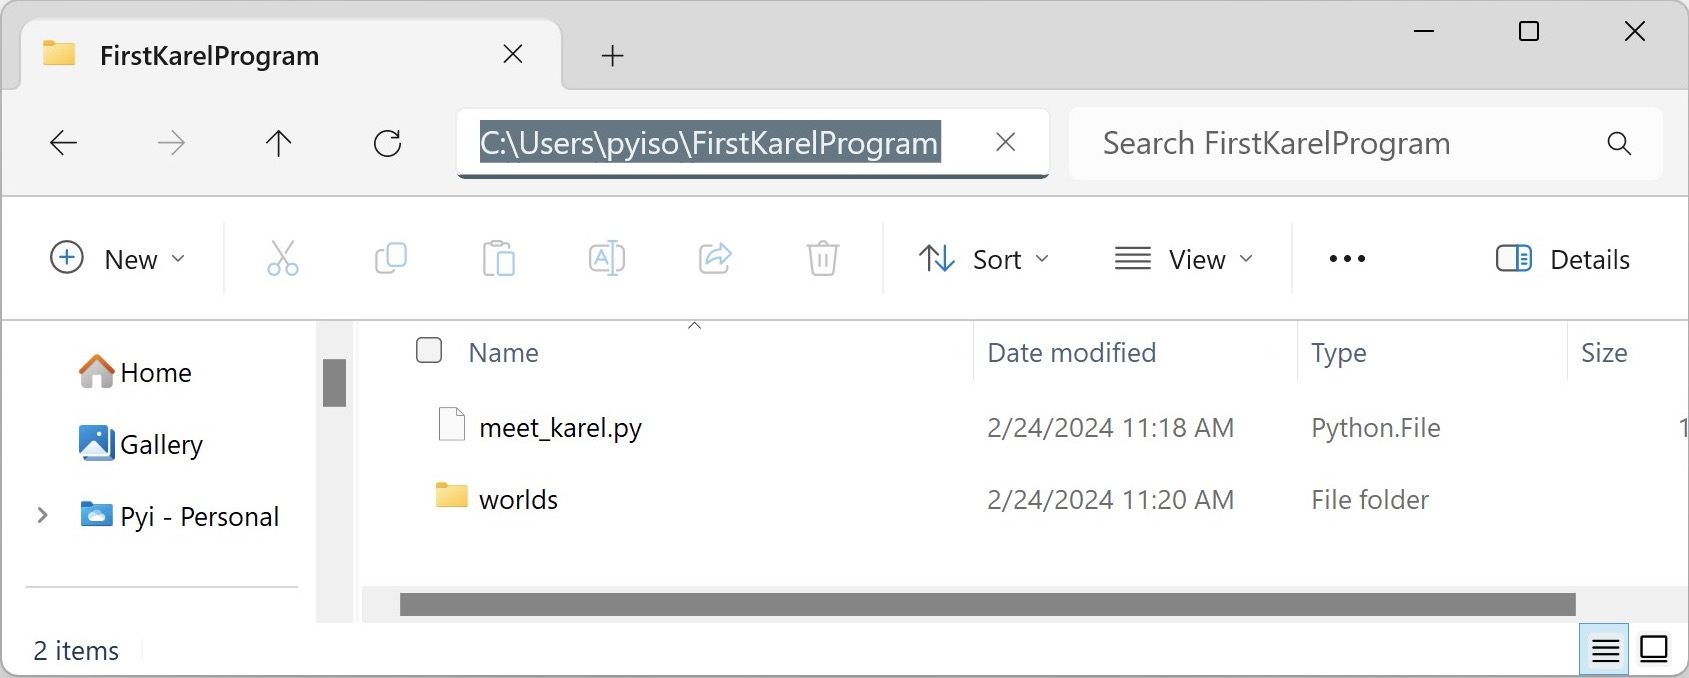
\includegraphics[width=.98\textwidth, trim={2.4mm 2mm 2mm 2mm},clip]{images/ch01/projstruct.jpg}};
    \drawshadow{image}
\end{tikzpicture}
\caption{} 
\label{fig:projstruct}
\end{figure}

\begin{figure}[tbh!]
\begin{tikzpicture}
    \node[anchor=south west,inner sep=0] (image) at (0,0)
        {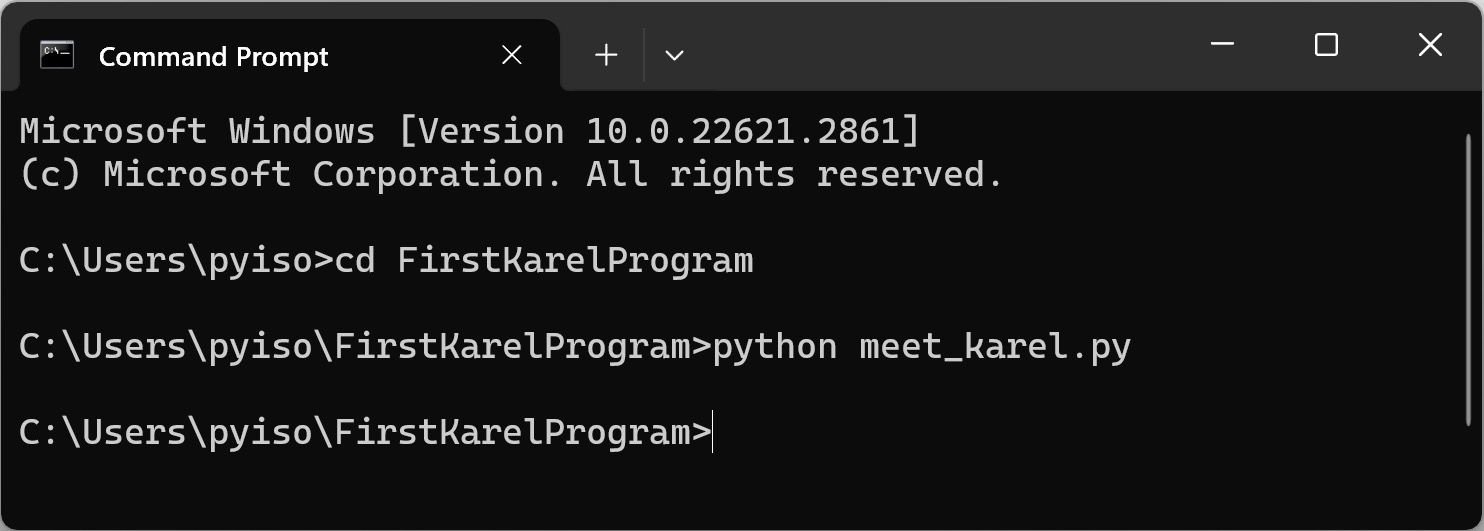
\includegraphics[width=.98\textwidth, trim={2.4mm 2mm 2mm 2mm},clip]{images/ch01/runkrl.jpg}};
    \drawshadow{image}
    \draw [draw=red, thick,rounded corners] (2.825,2.58) rectangle (6.65,2);
    \draw [draw=red, thick,rounded corners] (6.1,1.83) rectangle (10,1.25);

\end{tikzpicture}
\caption{} 
\label{fig:runkrl}
\end{figure}

\begin{figure}[tbh!]
\begin{tikzpicture}
    \node[anchor=south west,inner sep=0] (image) at (0,0)
        {\includegraphics[width=.98\textwidth, trim={2.4mm 2mm 2mm 2mm},clip]{images/ch01/mtkrlprgm.jpg}};
    \drawshadow{image}
\end{tikzpicture}
\caption{} 
\label{fig:mtkrlprgm1}
\end{figure}

\section{Move Beeper to Other Side}
ပရိုဂရမ်းမင်း လေ့လာတဲ့အခါ စာချည်းပဲ ဖတ်နေပြီး အမှန်တကယ် နားလည်သွားဖို့ဆိုတာ မဖြစ်နိုင်ပါဘူး။ လက်တွေ့ စမ်းသပ်ကြည့်၊ ရေးကြည့်မှပဲ တကယ် နားလည်လာမယ်။ တကယ်လည်း ကျွမ်းကျွမ်းကျင်ကျင် ရေးတတ်လာမှာပါ။ ဒါကြောင့် လက်တွေ့ရေးကြည့်ပါ။ များများ လေ့ကျင့်ပါ။ ဥပမာတွေကိုလည်း နားလည်အောင် ဖတ်ပြီးရင် မိမိဘာသာ အလွတ် ပြန်ရေးကြည့်ပါ။ 

ပုံ (\fRefNo{\ref{fig:mbtos}}) မှ ဘိပါကို နံရံအခြားတစ်ဘက် အောက်ခြေကို ရွှေ့ပေးတဲ့ ပရိုဂရမ် ရေးကြည့်ပါ။ \fEn{Python} ထုံးစံအရ \mytcboxinl{\fEnSnd{move\_beeper\_to\_other\_side.py}} ဖိုင်နဲ့ သိမ်းသင့်ပါတယ်။ \mytcboxinl{\fEnSnd{meet\_karel.zip}} ဖိုင်ထဲမှာပါတဲ့ \fEnSnd{worlds} ဖိုဒါမှာပဲ အခု ကမ္ဘာဖိုင် ထည့်ပေးထားပါတယ်။ \mytcboxinl{\fEnSnd{move\_beeper\_to\_other\_side.w}} နံမည်နဲ့ပါ။ အန်ထရီပွိုင့်အတွက် အခုလိုရေးရပါမယ်။

\setlength{\fboxsep}{0pt}
\begin{minted}[frame=\mintframe, framerule=\mintrule,framesep= \mintsep, xleftmargin=\xlftmargin
    , bgcolor=mintbgcolor,rulecolor=mintrulecolor
    , python3=true,escapeinside=ßß]{python}
if __name__ == "__main__":
    run_karel_program("move_beeper_to_other_side")
\end{minted}

\begin{figure}[tbh!]
\begin{tikzpicture}
    \node[anchor=south west,inner sep=0] (image) at (0,0)
        {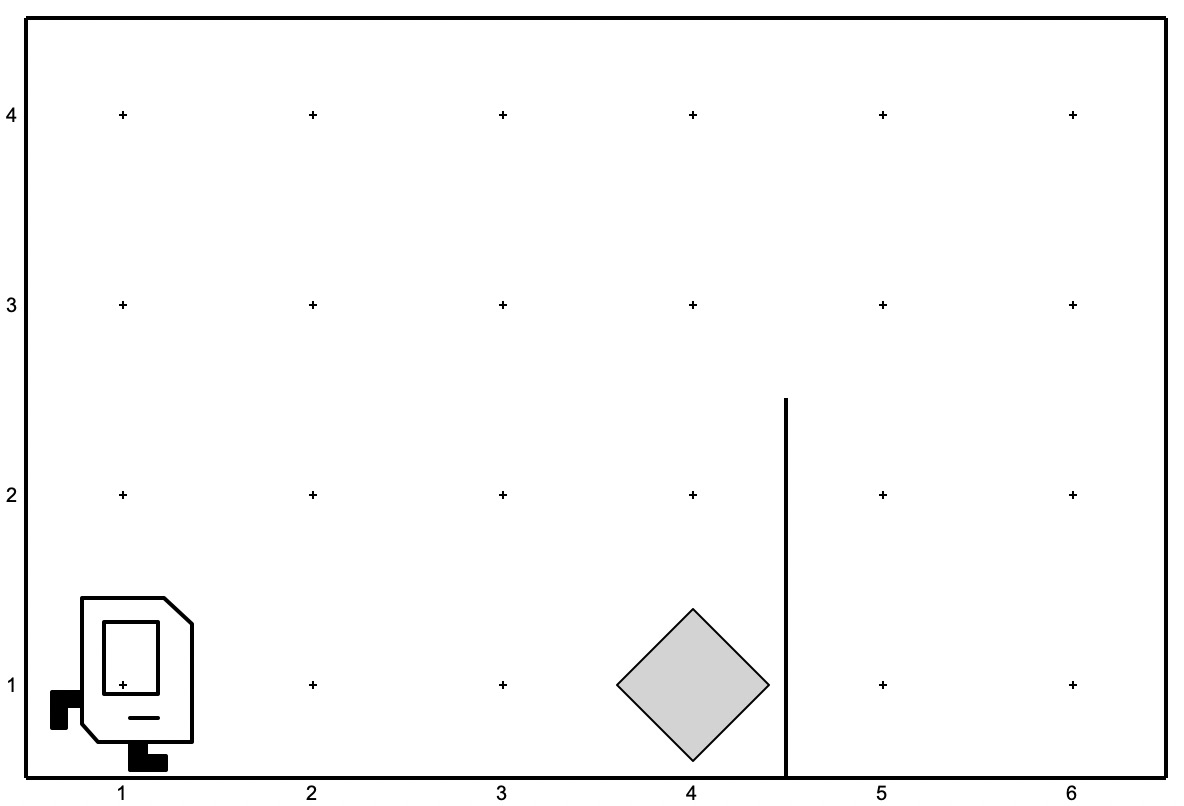
\includegraphics[width=3.5in, trim={2.4mm 2mm 2mm 2mm},clip]{images/ch01/MoveBeeperToOtherSide.jpg}};
    
\end{tikzpicture}
\caption{} 
\label{fig:mbtos}
\end{figure}


%

%

%
%
%
%အထက်ဖော်ပြပါ ပရိုဂရမ်ကုဒ် ပထမဆုံးတစ်ကြောင်းဟာ \fCode{import} စတိတ်မန့် ဖြစ်ပါတယ်။ ပရိုဂရမ်ကုဒ်ထဲမှာ ကလပ်စ် \fEn{(Class)} တစ်ခုကို ရည်ညွှန်းအသုံးပြုလို့ရအောင် \fCode{import} လုပ်ပေးရတာပါ။
%%
%\begin{minted}[frame=lines, framerule=0pt]{java}
%import stanford.karel.Karel;
%\end{minted}
%%
% \fCode{stanford.karel} \fOpn{ပက်ကေ့ချ်} \fEn{(package)} မှ \fCode{Karel} ကလပ်စ်ကို \fCode{import} လုပ်ထားတာ ဖြစ်တယ်။ စတိတ်မန့် အဆုံးမှာ ဆီမီးကော်လံ \fEn{(\fCode{;})} ပါတာကို သတိပြုပါ။ \fEn{Java} မှာ စတိတ်မန့် တစ်ကြောင်းဆုံးတိုင်း ဆီမီးကော်လံ ထည့်ပေးရပါမယ်။ \fOpn{ပက်ကေ့ချ်}ဆိုတာ ဆက်စပ်ရာ ကလပ်စ်တွေ စုစည်းထားတဲ့ ယူနစ်တစ်ခုပါပဲ။ \fCode{stanford.karel} \fOpn{ပက်ကေ့ချ်}ထဲက ကလပ်စ်အားလုံးကို \fCode{import} လုပ်မယ်ဆိုရင် ဒီလိုရေးရတယ်။
%%
%\begin{minted}[frame=lines, framerule=0pt]{java}
%import stanford.karel.*;
%\end{minted}
%%  
%လိုအပ်တဲ့ ကလပ်စ်ကိုပဲ ရွေးပြီး \fCode{import} လုပ်တာ ပိုကောင်းပါတယ်။
%
%\subsection*{ကလပ်စ်}
%ကလပ်စ် \fEn{(Class)} အကြောင်းကို နောက်ပိုင်းမှာ လေ့လာကြရမှာပါ။ အခုလောလောဆယ် ကလပ်စ်ကို ပရိုဂရမ်ကုဒ် စထရက်ချာတစ်မျိုးဟု ယူဆပါ။ \fEn{Java} ပရိုဂရမ်တစ်ခုမှာ အနည်းဆုံး ကလပ်စ်တစ်ခု ရှိရပါမယ်။ ကလပ်စ်တစ်ခုဖြစ်ဖို့အတွက် ဆင်းတက်စ်အရ အနည်းဆုံးရှိရမဲ့ ပုံစံက ဒီလိုပါ။
%%
%\begin{minted}[frame=lines, framerule=0pt]{java}
%public class MeetKarel {
%
%}
%\end{minted}
%% 
%ကလပ်စ်နံမည်က \fCode{MeetKarel} ဖြစ်ပါတယ်။ စကားလုံးအားလုံး အကြီးစာလုံးနဲ့ စထားတာ သတိထားကြည့်ပါ။ \fCode{meetkarel} လို့ရေးတာထက်  \fCode{MeetKarel} က စကားလုံးတစ်လုံးချင်းကို ပိုပြီးထင်ရှားစေတယ်။ ဒါကြောင့် အကြီးနဲ့စတဲ့ နည်းကိုပဲ အကြံပြုပါတယ်။
%
%\subsection*{\fSubSecCodeBf{Karel} ကလပ်စ်ကို \fSubSecCodeBf{extends} လုပ်ခြင်း}
%ရှေ့မှာတွေ့ခဲ့တဲ့ \fCode{MeetKarel} ကလပ်စ်ဟာ ကလပ်စ်အခွံချည်း ဖြစ်တယ်။ တွန့်ကွင်း အဖွင့်အပိတ်ကြားဟာ အလွတ်ဖြစ်နေပြီး ဘာပရိုဂရမ်ကုဒ်မှ မပါသေးပါဘူး။ ဒီကလပ်စ်ကို ကားရဲလ်ပရိုဂရမ်ဖြစ်အောင် အခုလိုရေးရပါမယ်။
%%
%\begin{minted}[frame=lines, framerule=0pt]{java}
%import stanford.karel.Karel;
%
%public class MeetKarel extends Karel {
%    
%}
%\end{minted}
%%
%\fCode{MeetKarel} ကလပ်စ်ဟာ \fCode{Karel} ကလပ်စ်ကို \fCode{extends} လုပ်ထားပါတယ်။ ပရိုဂရမ်ကုဒ်မှာ \fCode{Karel} ကလပ်စ်ကို ရည်ညွှန်းအသုံးပြုနိုင်ဖို့ အပေါ်မှာ \fCode{import} လုပ်ထားရတာပါ။ အခုအတိုင်းပဲ \fCode{MeetKarel}  ကို \fEn{IntelliJ} မှာ \fEn{run} ကြည့်ရင် ပုံ (\fRefNo{\ref{fig:meet_karel_window}}) မှာပြထားတဲ့ ကားရဲလ်ပရိုဂရမ် \fEn{window} တက်လာတာ တွေ့ရမှာပါ။ အဲဒီလိုမျိုး ကားရဲလ်ကမ္ဘာနဲ့ ဂရပ်ဖစ် \fEn{window} စခရင်ပေါ်မှာ ပေါ်လာတာဟာ  \fCode{Karel} ကလပ်စ်ထဲမှာ ပရိုဂရမ် ရေးပေးထားတဲ့ အတွက်ကြောင့် ဖြစ်တယ်။
%
%မှတ်ချက်။\qquad ။ အခုကစပြီး စာချည်းပဲဖတ်မနေဘဲ လက်တွေ့ပါ လိုက်လုပ်ကြည့်ဖို့ အလေးအနက် အကြံပြုချင်ပါတယ်။ စာမျက်နှာ \fRefNo{\pageref{apdx1}} နောက်ဆက်တွဲ (က) မှာ ဖော်ပြထားတဲ့အတိုင်း လိုအပ်တဲ့ ဆော့ဖ်ဝဲတွေထည့်သွင်းပါ။ နမူနာပါတဲ့ \fCode{MeetKarel} ပရိုဂရမ်ကို \fEn{run} ကြည့်ပါ။ 
%
%\begin{figure}[tb!]
%\begin{tikzpicture}
%    \node[anchor=south west,inner sep=0] (image) at (0,0)
%        {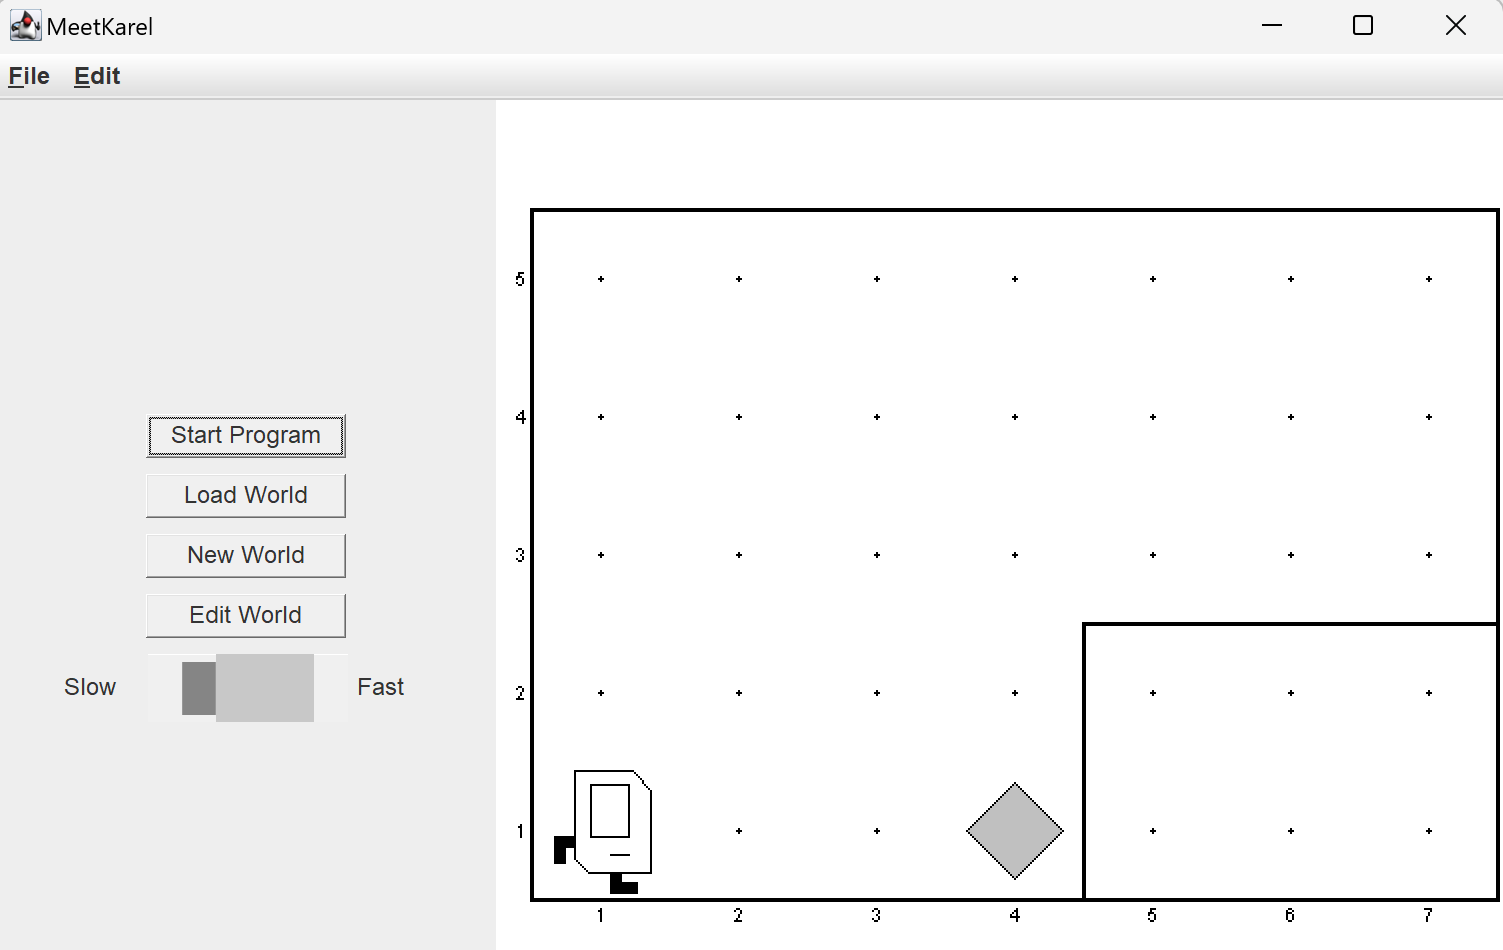
\includegraphics[width=.9\linewidth]{images/intellij_proj_create/MeetKarel.png}};
%    \drawshadow{image}
%\end{tikzpicture}
%\caption{}
%\label{fig:meet_karel_window}
%\end{figure}
%
%\subsection*{\fSubSecCodeBf{run} မက်သဒ်}
%
%မက်သဒ်ဆိုတာ စတိတ်မန့်တစ်စုကို ယူနစ်တစ်ခုအနေနဲ့ ဖွဲ့စည်းထားဖို့ အသုံးပြုတဲ့ စထရက်ချာတစ်မျိုးပါပဲ။ \fCode{move} စတိတ်မန့် သုံးခုကို ယူနစ်တစ်ခုအဖြစ် စုဖွဲ့ပေးထားတဲ့ \fCode{run} မက်သဒ်ကို အခုလိုတွေ့ရပါမယ်။ 
%%
%\begin{minted}[frame=lines, framerule=0pt]{java}
%import stanford.karel.Karel;
%
%public class MeetKarel extends Karel {
%    public void run() {
%        move();
%        move();
%        move();
%    }
%}
%\end{minted}
%%
%\fCode{run} မက်သဒ်ဟာ ကလပ်စ်ဘော်ဒီထဲမှာ ရှိရပါမယ်။ \fCode{run} ကို ဘယ်သူမဆို သုံးလို့ရအောင် \fCode{public} မက်သဒ်အနေနဲ့ သတ်မှတ်ထားတယ်။ \fCode{run} ဟာ \fCode{void} မက်သဒ်လည်းဖြစ်တယ်။ ဘာတန်ဖိုးမှ ပြန်ထုတ်မပေးတဲ့ မက်သဒ်လို့ အဓိပ္ပါယ်ရတယ်။  မက်သဒ်နံမည် \fCode{run} ဘေးမှာ ဝိုက်ကွင်းတစ်စုံပါရမယ်။ တွန့်ကွင်းတစ်စုံကတော့ မက်သဒ်ဘော်ဒီ အစနဲ့အဆုံးကို သတ်မှတ်ပေးထားတာ။ မက်သဒ်ဘော်ဒီထဲမှာ သက်ဆိုင်တဲ့ စတိတ်မန့်တွေ ရေးပေးရမယ်။ မက်သဒ်တွေအကြောင်း တစ်ခန်းသတ်သတ် လေ့လာကြရမှာပါ။ အဲဒီကျရင် အခုသိပ်နားမလည်တာတွေ အားလုံးရှင်းသွားပါလိမ့်မယ်။
%
%\fCode{run} ဟာ ကားရဲလ်ပရိုဂရမ်တွေအတွက် အထူးစီမံထားတဲ့ မက်သဒ်တစ်ခု ဖြစ်တယ်။ ပုံ (\fRefNo{\ref{fig:meet_karel_window}}) ကားရဲလ်ပရိုဂရမ် \fEn{window} ပေါ်လာပြီး \fEn{“Start Program”} နှိပ်လိုက်ရင် \fCode{run} မက်သဒ်ကို လုပ်ဆောင်ပေးတယ်။ \fEn{“Start Program”} မနှိပ်သေးရင် \fCode{run} နဲ့ဆိုင်တဲ့ စတိတ်မန့်တွေကလည်း အလုပ်မလုပ်သေးပါဘူး။ နှိပ်လိုက်တော့မှ \fCode{run} က စပြီးအလုပ်လုပ်တာပါ။ \fEn{“Start Program”} နှိပ်တဲ့အခါတိုင်း \fCode{run} ကို လုပ်ဆောင်ပေးမှာပါ။ 
%
%\fCode{MeetKarel} ကို အပေါ်မှာ ပြထားတဲ့အတိုင်း \fEn{IntelliJ} မှာ ရေးပြီး \fEn{run} ကြည့်ပါ။ \fEn{“Start Program”} နှိပ်လိုက်ရင် ကားရဲလ်က ရှေ့ကို သုံးခါရွှေ့ပေးပါလိမ့်မယ်။ နောက်ထပ်တစ်ခါ ထပ်နှိပ်ရင် \fCode{run} ကလည်း တစ်ခါထပ် အလုပ်လုပ်မှာပါ။ ဒါပေမဲ့ ရှေ့မှာ နံရံပိတ်နေတဲ့အတွက် ရွှေ့လို့မရတော့ဘဲ အယ်ရာတက်ပါလိမ့်မယ်။ \fEn{“Load World”} ကို နှိပ်ပြီး \fEn{MeetKarel.w} ဖိုင်ကိုရွေးလိုက်ရင် နဂိုအနေအထားပြန်ဖြစ်သွားပါလိမ့်မယ်။ ဒါမှမဟုတ် ပရိုဂရမ်ကို ပိတ်ပြီး ပြန် \fEn{run} နိုင်ပါတယ်။
%
%\subsection*{မက်သဒ်ကောလ် စတိတ်မန့်}
%\fCode{run} မက်သဒ်ထဲမှာတွေ့ရတဲ့ စတိတ်မန့်တွေဟာ မက်သဒ်ကောလ် \fEn{(method call)} စတိတ်မန့်တွေဖြစ်ပါတယ်။ \fCode{move}\fEn{,} \fCode{pickBeeper}\fEn{,}  \fCode{putBeeper}\fEn{,} \fCode{turnLeft} ကွန်မန်းတွေဟာ \fCode{Karel} ကလပ်စ်မှာ သတ်မှတ်ပေးထားတဲ့ မက်သဒ်တွေဖြစ်တယ်။ ပရိုဂရမ်ရေးတဲ့အခါ ကားရဲလ်ကွန်မန်းတွေကို မက်သဒ်ကောလ် စတိတ်မန့်အနေနဲ့ ရေးရမယ်။ ဥပမာ ဘယ်ဘက် လှည့်ခိုင်းတာကို
%%
%\begin{minted}[frame=lines, framerule=0pt]{java}
%turnLeft();
%\end{minted}
%%
%လို့ ရေးရပါမယ်။ စတိတ်မန့်ဖြစ်တဲ့အတွက် ဆီမီးကော်လံချပေးရမှာ ဂရုပြုပါ။ 
%
%\subsection*{မှတ်ချက်ရေးခြင်း}
%ဘိပါကို နေရာရွှေ့ထားဖို့ အပြီးထိဆက်ရေးထားတဲ့ ပရိုဂရမ်ကို အောက်မှာ ပြန်ဖော်ပြပေးထားပါတယ်။ မှတ်ချက် \fEn{(comment)} ရေးထားတာ တချို့ ပါနေတာကလွဲရင် စာမျက်နှာ \fRefNo{\pageref{lst:MeetKarel1}} မှာ ဖော်ပြခဲ့တဲ့ ပရိုဂရမ်နဲ့ တူတူပါပဲ။
%%
%\begin{minted}[frame=lines, framerule=0pt]{java}
%/* 
%This is our first example Karel program. This program is for 
%moving the beeper to(5,3) corner.
%*/
%import stanford.karel.Karel;
%
%public class MeetKarel extends Karel {
%    public void run() {
%        move();
%        move();
%        move();
%        pickBeeper();
%        turnLeft();
%        move();
%        move();
%        // we want karel to turn right
%        // turning left 3 times is the same as turning right
%        turnLeft();
%        turnLeft();
%        turnLeft();
%        move();
%        putBeeper();
%    }
%}
%\end{minted}
%% 
%ကွန်းမန့်ရေးချင်ရင် \fCode{/*} နဲ့ \fCode{*/} အတွင်း သို့မဟုတ် \fCode{//} နောက်မှာ ရေးရပါတယ်။ ကွန်းမန့်တွေကို ပရိုဂရမ်ကုဒ်အနေနဲ့ မယူဆရပါဘူး။ တနည်းအားဖြင့် ကွန်းမန့်တွေဟာ ကွန်ပျူတာ ဆောက်ရွက်ပေးရမဲ့ ညွှန်ကြားချက်တွေ မဟုတ်ပါဘူး။ ပရိုဂရမ်ကုဒ်ကို နားလည်အောင်ရှင်းပြတာ သို့မဟုတ် ဘယ်လိုစဉ်းစားပြီး ရေးခဲ့တာလည်း နောင်တချိန်ပြန်ဖတ်တဲ့အခါ မှတ်မိအောင် ပရိုဂရမ်ကုဒ်ထဲမှာ ကွန်းမန့်ရေးထားရလေ့ရှိပါတယ်။
%
%\fCode{/*} နဲ့ \fCode{*/} အတွင်း ရေးထားတဲ့ စာကြောင်းအားလုံးကို ကွန်းမန့်အနေနဲ့ယူဆတယ်။ \fEn{Multiline comment} အတွက် သုံးတာဖြစ်တယ်။ ဥပမာ
%%
%\begin{minted}[frame=lines, framerule=0pt]{java}
%/*
%This is the first line of comment.
%This is the second line of comment
%*/
%\end{minted}
%%
%\fCode{//} ကတော့ နောက်မှာရှိတဲ့ စာကြောင်းကိုပဲ ကွန်းမန့်အနေနဲ့ ယူဆတာ။ ဥပမာ
%%
%\begin{minted}[frame=lines, framerule=0pt]{java}
%pickBeeper(); // to pick the beeper at the current corner if any
%turnLeft();
%\end{minted}
%%
%ဒီနှစ်ကြောင်းမှာ \fCode{pickBeeper} နဲ့ \fCode{turnLeft} စတိတ်မန့်တွေဟာ ကွန်းမန့်မဟုတ်ပါ။  ပထမတစ်ကြောင်း နောက်ပိုင်း စာလုံးအစောင်းနဲ့ စာသားတွေကပဲ ကွန်းမန့်ဖြစ်ပါတယ်။  
%%
%\begin{minted}[frame=lines, framerule=0pt]{java}
%pickBeeper(); // to pick the beeper at the current corner if any
%// turnLeft();
%\end{minted}
%%
%ဒီလိုဆိုရင်တော့ ဒုတိယအကြောင်း \fCode{turnLeft} ကလည်း ကွန်းမန့်ဖြစ်သွားပါမယ်။
%
%\section{လေ့ကျင့်ရန် ပရိုဂရမ်}
%အခြားအခြားသော ပညာရပ်တွေလိုပဲ ပရိုဂရမ်ရေးတာဟာလည်း စာဖတ်နေရုံနဲ့ ကျွမ်းကျင်တတ်မြောက်သွားမဲ့ ပညာရပ်မျိုး မဟုတ်ပါဘူး။ လက်တွေ့ရေးပြီး အချိန်ပေး လေ့ကျင့်ဖို့ လိုအပ်တယ်။ များများရေး များများလေ့ကျင့်မှ ကျွမ်းကျင်လာမယ်။ ဒီအတွက် လိုအပ်တဲ့ ဆော့ဖ်ဝဲတွေ ထည့်ထားရပါမယ်။ စာမျက်နှာ \fRefNo{\pageref{apdx1}} နောက်ဆက်တွဲ (က) ကိုဖတ်ပြီး ဆော့ဖ်ဝဲတွေ သွင်းပါ။ ပရောဂျက်အသစ်၊ ကလပ်စ်အသစ် ဖန်တီးနည်းတို့ကိုလည်း နောက်ဆက်တွဲ (က) မှာ အသေးစိတ်ဖော်ပြပေးထားပါတယ်။ အခုပဲ သွားဖတ်ပြီး လက်တွေ့လိုက်လုပ်ပါလို့ အကြံပြုချင်ပါတယ်။
%
%ဒီအခန်းအတွက် နမူနာပရောဂျက် ထည့်ပြီးသွားရင် နောက်ဆက်တွဲ (က) စာမျက်နှာ \fRefNo{\pageref{apdx1:new_class}} မှာ ဖော်ပြထားတဲ့အတိုင်း ကလပ်စ်အသစ်ဖန်တီးယူပါ။ ပုံမှာတွေ့ရတဲ့ ဘိပါကို နံရံအခြားတစ်ဘက် မြှားပြထားတဲ့နေရာကို ရွှေ့ပေးတဲ့ ပရိုဂရမ် ရေးပါ။
%
%\begin{figure}[htb!]
%\begin{tikzonimage}[width=4in]{images/ch01/MoveBeeperToOtherSide.jpg}%[tsx/show help lines]
%    \draw[-{Latex[length=3mm]}] (0.85 ,0.27)--(0.75, 0.16);
%\end{tikzonimage}
%\caption{\fCptCodeBf{MoveBeeperToOtherSide} ကမ္ဘာ}
%\label{fig:move_beeper_to_other_side1}
%\end{figure}
%
%\subsection*{ကားရဲလ်ကမ္ဘာ ဖိုင် (Karel's World File)}
%ဒီပရိုဂရမ်အတွက် ကလပ်စ်နံမည်ကို \fCode{MoveBeeperToOtherSide} ပေးပါလို့ ပြောထားတာ အကြောင်းရှိပါတယ်။ အမှန်က ကားရဲလ်ပရိုဂရမ်တစ်ခုမှာ သင့်တော်တဲ့ ကလပ်စ်နံမည် စိတ်ကြိုက်ရွေးချယ် ပေးလို့ရပါတယ်။ ဒါပေမဲ့ ပရိုဂရမ် \fEn{run} လိုက်ရင် ပေါ်လာတဲ့ကမ္ဘာက အခုပုံမှာတွေ့ရတာနဲ့ တူမှာမဟုတ်ဘူး။ အခုပြထားတဲ့ကမ္ဘာပုံဖြစ်အောင် \fEn{worlds} ဖိုဒါထဲက \fEn{MoveBeeperToOtherSide.w} ဖိုင်မှာ သတ်မှတ်ပေးထားရတာပါ။ \fCode{MeetKarel} ကမ္ဘာပုံဖြစ်အောင် အဲ့ဒီဖိုဒါထဲကပဲ \fEn{MeetKarel.w} မှာ သတ်မှတ်ပေးထားတာ။ ကားရဲလ်ပရိုဂရမ် ကလပ်စ်တစ်ခုကို \fEn{run} တဲ့အခါ ကလပ်စ်နံမည်နဲ့ တူတဲ့ \fEnEmpBf{.w} ဖိုင်ကိုရှာပြီး အဲဒီဖိုင်မှာသတ်မှတ်ထားတဲ့ ကမ္ဘာကို တင်ပေးတာပါ။ နံမည်တူရှာမတွေ့ရင်တော့ \(10 \times 10\) အရွယ် \fEn{default} ကမ္ဘာကို  တင်ပေးမှာပါ။ \fEn{“Load World”} နှိပ်ပြီး \fEn{worlds} ဖိုဒါထဲက လိုချင်တဲ့ ကမ္ဘာကို ခေါ်တင်လို့ရတယ်။ ပရိုဂရမ် \fEn{run} လိုက်၊ လိုချင်တဲ့ကမ္ဘာကို ခေါ်တင်လိုက်နဲ့ ကရိကထများမယ်။ ဒါကြောင့် ကမ္ဘာနံမည်နဲ့ ကလပ်စ်နံမည် တူအောင်ပေးခိုင်းရတာ ဖြစ်တယ်။
%
%\section{ဖြစ်လေ့ရှိတဲ့ အမှားတချို့}
%
%အခုမှ ပရိုဂရမ်စရေးဖူးတဲ့ လူသစ်တွေ ဖြစ်လေ့ရှိတဲ့ အမှားတချို့ကို ဆက်လက်ဖော်ပြပါမယ်။
%
%\subsection*{တွန့်ကွင်းကျန်ခဲ့ခြင်း}
%ကလပ်စ်ဘော်ဒီ၊ မက်သဒ်ဘော်ဒီတို့ရဲ့ အစ အဆုံးကို တွန့်ကွင်း အဖွင့် အပိတ်နဲ့ သတ်မှတ်ပေးရတာပါ။ အဖွင့် သို့မဟုတ် အပိတ် တွန့်ကွင်း ကျန်ခဲ့ရင် ဆင်းတက်စ်အမှားဖြစ်ပြီး ပရိုဂရမ်ကို \fEn{run} လို့ရမှာ မဟုတ်ပါဘူး။ အပြင်ဆုံးမှာ ကလပ်စ်ဘော်ဒီအတွက် တွန့်ကွင်းတစ်စုံ၊ ကလပ်စ်ဘော်ဒီထဲက \fCode{run} မက်သဒ်ဘော်ဒီအတွက် တွန့်ကွင်းတစ်စုံ ရှိရမှာဖြစ်တယ်။
%
%အဖွင့်အပိတ် မစုံရင် \fEn{IntelliJ} က ကုဒ်ရေးတဲ့ \fEn{editor} မှာရော ပရောဂျက်ဖိုဒါမှာပါ အယ်ရာပြပေးပါတယ်။ တွန့်ကွင်းကျန်ခဲ့လို့ ဖြစ်တာဆိုရင် ဖြည့်ပေးလိုက်ရင် အယ်ရာတွေမပြတော့ပါဘူး။ ဆက်ပြနေသေးရင် အခြားအကြောင်းကြောင့်ဖြစ်တာ ဖြစ်နိုင်ပါတယ်။
%
%\subsection*{ဆီမီးကော်လံ ကျန်ခဲ့ခြင်း}
%\fCode{import} စတိတ်မန့်၊ မက်သဒ်ကောလ်စတိတ်မန့် တွေမှာ ဆီမီးကော်လံနဲ့ ဆုံးပေးရပါမယ်။ ကျန်ခဲ့ရင် ဆင်းတက်စ်အယ်ရာဖြစ်ပြီး \fEn{run} လို့ရမှာ မဟုတ်ပါ။ 
%
%\subsection*{ဝိုက်ကွင်းကျန်ခဲ့ခြင်း}
%\fCode{run} မက်သဒ်သတ်မှတ်ချက်မှာ ဝိုက်ကွင်းအဖွင့်အပိတ် တစ်စုံပါရမယ်။ မက်သဒ်ကောလ် စတိတ်မန့်တွေမှာလည်း ဝိုက်ကွင်းတစ်စုံ ပါရပါမယ်။
%
%\subsection*{စာလုံးအကြီးအသေး၊ စာလုံးပေါင်းနှင့် နံမည်ပေးခြင်း}
%\fEn{Java} မှာ နံမည်တွေ စာလုံး အကြီးအသေး လွဲလို့မရပါဘူး။ \fEn{“Case Sensitive”} ဖြစ်တယ်လို့ ခေါ်ပါတယ်။ မက်သဒ်ကောလ်လုပ်တဲ့ စတိတ်မန့်တွေမှာ စာလုံးပေါင်းရော အကြီးအသေးပါ ဂရုစိုက်ရေးဖို့လိုပါတယ်။ ဥပမာ ဒီလိုတွေရေးရင် အယ်ရာဖြစ်မှာပါ။
%%
%\begin{minted}[frame=lines, framerule=0pt,escapeinside=ßß]{text}
%turnleft();    //ß l \fMM{အသေးဖြစ်နေ}ß 
%PickBeeper();  //ß P \fMM{အကြီးဖြစ်နေ}ß 
%turn Left();   //ß \fMM{စပေ့စ်ပါနေတယ်}ß
%\end{minted}
%% 
%\fEn{IntelliJ} ရဲ့ \fEn{Code Completion} ဖီချာက ဒီလိုအမှားမျိုးနည်းအောင် ကူညီပေးပါတယ်။
%
%နံမည်ပေးတာရယ်၊ ပေးထားတဲ့နံမည်နဲ့ ရည်ညွှန်းအသုံးပြုတာရယ် ကိစ္စနှစ်ခုကို ခွဲခြားပြောဖို့လိုပါတယ်။ ကလပ်စ်သတ်မှတ်တဲ့အခါနဲ့ မက်သဒ်သတ်မှတ်တဲ့အခါမှာ ကလပ်စ်နံမည်၊ မက်သဒ်နံမည် ပေးရပါတယ်။ နံမည်ပေးတဲ့အခါ လိုက်နာဖို့ လိုအပ်တာတွေရှိပါတယ်။ နံမည်က ဂဏန်းနဲ့စလို့မရပါဘူး။ နံမည်မှာ စပေ့စ်ပါလို့မရဘူး။ ဥပမာ ဒီလိုတွေမရပါဘူး။
%%
%\begin{minted}[frame=lines, framerule=0pt,escapeinside=ßß]{java}
%public class ß\color{blue}\fCodeBf{1stKarelExample}ß ß\fCode{\bropn ...}ß 
%\end{minted}
%%
%%
%\begin{minted}[frame=lines, framerule=0pt,escapeinside=ßß]{java}
%public class ß\color{blue}\fCodeBf{Meet Karel}ß ß\fCode{\bropn ...}ß
%\end{minted}
%%
%ဒါကနံမည်ပေးတဲ့အခါ လိုက်နာဖို့လိုတဲ့ စည်းမျဉ်းတချို့ပါ။ အသေးစိတ်ကို နောက်ပိုင်းမှာ ဆက်လေ့လာရမှာပါ။ 
%
%နောက်တစ်ခုက နံမည်နဲ့ ရည်ညွှန်းအသုံးပြုတာပါ။ \fCode{turnLeft} မက်သဒ်ကို \fCode{Karel} ကလပ်စ်ထဲမှာ သတ်မှတ်ထားတယ်လို့ ပြောခဲ့တယ်။ \fCode{turnLeft} နံမည်နဲ့ပဲ မက်သဒ်ကောလ် လုပ်ရပါမယ်။ ဒါဟာ မက်သဒ်နံမည်နဲ့ မက်သဒ်ကို ရည်ညွှန်းအသုံးပြုတာပါ။ ပေးထားတဲ့နံမည်အတိုင်း အတိအကျရေးပြီး ရည်ညွှန်းအသုံးပြုရပါမယ်။ လွဲလို့မရပါဘူး။ ကလပ်စ်နံမည်လည်း ထိုနည်းတူစွာပါပဲ။ \fCode{Karel} ကလပ်စ်ကို ရည်ညွှန်းအသုံးပြုတဲ့အခါ နံမည်စာလုံးပေါင်းတာ တိကျဖို့ လိုပါတယ်။
%
%\fCode{run} မက်သဒ်ကို \fCode{Run} လို့နံမည်ပေးမိရင်လည်း ပြဿနာရှိပါတယ်။ \fEn{“Start Program”} နှိပ်ရင် \fCode{run} (စာလုံးအသေး) နံမည်နဲ့ မက်သဒ်ကို လုပ်ဆောင်ပေးတာပါ။ \fCode{Run} ဖြစ်နေရင် အဲ့ဒီမက်သဒ်က အလုပ်လုပ်မှာ မဟုတ်ပါဘူး။
\chapter{title}\label{ch:ch02}
\chapter{ဖန်ရှင်များ (Functions)}\label{ch:ch03}

ဖန်ရှင် \fEn{(\textit{function})} တွေဟာ ပရိုဂရမ်းမင်းမှာ အရေးကြီးဆုံး အခြေခံသဘောတရားတစ်ခု ဖြစ်တယ်။ ဖန်ရှင်ဆိုတာ ဘာလဲ၊ ဘာကြောင့် အရေးပါရတာလဲ၊ ဖန်ရှင်တွေကို ပရိုဂရမ် ဒီဇိုင်းပြုလုပ် ရေးသားတဲ့အခါ ဘယ်လိုအသုံးချတာလဲ စတာတွေကို ဒီအခန်းမှာ လေ့လာကြပါမယ်။

\section{ဖန်ရှင် သတ်မှတ်ခြင်း}
ညာဘက် လှည့်ခိုင်းချင်တိုင်း \fCode{turn\_left} သုံးခါရေးနေရတာ ရေရှည်အဆင်မပြေပါဘူး။ \fCode{turn\_right} လို့ပဲ တိုက်ရိုက် ရေးလို့ရရင် ပိုပြီးတော့ အဆင်ပြေမှာပါ။ ဒီလို လိုအပ်ချက်မျိုးကို ဖြည့်ဆည်း ပေးဖို့အတွက်ဟာ ဖန်ရှင်တွေရဲ့ အဓိက ရည်ရွယ်ချက်တွေထဲက တစ်ခုဖြစ်တယ်။ \fCode{turn\_right} ဖန်ရှင်ကို အခုလို သတ်မှတ်နိုင်ပါတယ်။
%
\begin{py}
def turn_right():
    turn_left()
    turn_left()
    turn_left()
\end{py}
%
ဒီလို သတ်မှတ်ထားပြီးရင် ညာဘက်လှည့်ချင်တဲ့အခါ 
%
\begin{py}
turn_right()
\end{py}
%
လို့ တိုက်ရိုက်ပြောလို့ ရသွားမှာ ဖြစ်ပါတယ်။ \fCode{turn\_left} သုံးခါ ရေးဖို့ မလိုတော့ပါဘူး။

ဖန်ရှင်တစ်ခု သတ်မှတ်တယ် \fEn{(\textit{defining a function})} ဆိုတာ ကိစ္စတစ်ခု ဖြေရှင်းဆောင်ရွက်ဖို့အတွက် စတိတ်မန့်တွေကို ယူနစ်တစ်ခုအဖြစ် ဖွဲ့စည်းထားလိုက်တာပါပဲ။ ၎င်းယူနစ်အတွက် အမည်တစ်ခုကိုလည်း သတ်မှတ်ပေးတယ်။ 

ဖန်ရှင် သတ်မှတ်မယ် ဆိုရင် \fCodeBf{def} \fEn{keyword} သုံးရပါတယ်။ အထက်ပါ \fCode{turn\_right} ဖန်ရှင် သတ်မှတ်ချက် \fEn{(\textit{function definition})} မှာ 
%
\begin{py}
def turn_right():
\end{py}
%
ကို ဖန်ရှင် ဟက်ဒ်ဒါ \fEn{(\textit{function header})} လို့ ခေါ်တယ် (မြန်မာလို ဆိုရင်တော့ ဖန်ရှင် ခေါင်းစည်းပေါ့)။ \fCode{turn\_right} က ဖန်ရှင် အမည်။ ပါရာမီတာပါတဲ့ ဖန်ရှင်ဆိုရင် ဝိုက်ကွင်းထဲမှာ ပါရာမီတာတွေ သတ်မှတ်ရတယ်။ ဥပမာ \fEn{\fCode{(x, y)}}။ ပါရာမီတာ မပါရင်တော့ \fEn{\fCode{()}} ပဲဖြစ်မယ်။ ကားရဲလ်မှာ ဖန်ရှင်အားလုံးဟာ ပါရာမီတာ မပါတဲ့အတွက် \fEn{\fCode{()}} ပဲ ဖြစ်မှာပါ။ ဖန်ရှင်ဟက်ဒ်ဒါ လိုင်းအဆုံးမှာ ကော်လံ \fEn{‘\fCode{:}’} ထည့်ပေးဖို့ လိုပါတယ်။ \todo{ပါရာမီတာတွေကို ဘယ်အခန်းမှာ လေ့လာမလဲပြောရန်}

ဖန်ရှင် ဟက်ဒ်ဒါအောက် အင်ဒန့်ထ်လုပ်ထားတဲ့ လိုင်းအားလုံးဟာ ၎င်းဖန်ရှင်နဲ့ သက်ဆိုင်တဲ့ ကုဒ်ဘလောက် ဖြစ်တယ်။ အခု \fCode{turn\_right} ဖန်ရှင် ဘလောက်မှာ \fCode{turn\_left} သုံးကြိမ်ပါတယ်။ 
%
\begin{py}
turn_right()
\end{py}
%
လုပ်ခိုင်းတာက (သတ်မှတ်ထားတဲ့) ဖန်ရှင်ကို အသုံးပြုတာ ဖြစ်တယ်။ ဒီအခါမှာ ၎င်းဖန်ရှင်နဲ့ သက်ဆိုင်တဲ့ ဘလောက်ကို လုပ်ဆောင်ပေးမှာပါ။ ဖန်ရှင်ကို အသုံးပြုတာကို ဖန်ရှင်ကောလ် \fEn{(\textit{function call})} လုပ်တယ်လို့ ပြောပါတယ်။ (မြန်မာလိုတော့ ‘ဖန်ရှင်ခေါ်’ တယ်လို့ ပြောတာပေါ့)။

ဖန်ရှင်သတ်မှတ်တာနဲ့ ဖန်ရှင်ကောလ် လုပ်တဲ့ပုံစံကို အောက်ပါအတိုင်း ယေဘုယျအားဖြင့် တွေ့ရပါမယ်။ \fEn{Python} ထုံးစံအရ ဖန်ရှင်နံမည်မှာ စာလုံးအသေးကိုပဲ သုံးလေ့ရှိတယ်။ စကားလုံး နှစ်ခုနဲ့ အထက်ဆိုရင် ကြားမှာ \fEn{underscore (\textunderscore)} ခြားပေးလေ့ ရှိတယ်။ 
%
\begin{py}
def ß$name\fEn{\textunderscore}of\fEn{\textunderscore}function$ß():
    ß$statement_1$ß
    ß$statement_2$ß
    ß$statement_3$ \fEn{etc.}ß
\end{py}
%
%
%
\begin{py}
ß$name\fEn{\textunderscore}of\fEn{\textunderscore}function$ß()
\end{py}
%

\begin{mytcboxflt}
\noindent \fSubSec{\textbf{ဖန်ရှင်နံမည် အဓိပ္ပါယ် အရေးကြီးပါတယ်}}
\betweentcboxpar
\noindent စာရေးတာပဲဖြစ်ဖြစ်၊ ပရိုဂရမ်ကုဒ် ရေးတာပဲဖြစ်ဖြစ် စိတ်ထဲ တွေးတဲ့အတိုင်း၊ စဉ်းစားတဲ့အတိုင်း ပေါ်လွင်အောင် ဖော်ပြနိုင်တာဟာ အားသာချက်တစ်ခုပါပဲ။ ဖန်ရှင် သတ်မှတ်ထားခြင်း အားဖြင့် ညာဘက်လှည့်ခိုင်းရင် \fCode{turn\_right} ဘိပါ နှစ်ဆယ့်ငါးခု ချရင် \fCode{put\_25\_beepers}  တိုက်ရိုက် ဖော်ပြလို့ ရတာဟာ အရေးပါတဲ့ ကိစ္စဖြစ်ပါတယ်။ ဘာသာစကားတစ်ခုရဲ့ ဖော်ပြနိုင်စွမ်း ‘အား’ \fEn{(expressive power)} ကို ထပ်လောင်းအားဖြည့်ပေးတာလို့ ဆိုရမှာပါ။
\betweentcboxpar

ဖန်ရှင်လုပ်ဆောင်ပေးတဲ့ ကိစ္စကို သိသာစေမဲ့၊ နားလည်ရလွယ်မဲ့ နံမည်မျိုး ဂရုစိုက်ရွေးချယ်တာကလည်း အရေးပါပါတယ်။ ကားရဲလ်ပရိုဂရမ်တွေမှာ အမိန့်ပေးခိုင်းစေတဲ့ ပုံစံနဲ့ ဖန်ရှင်နံမည်ပေးလေ့ရှိတယ်။ ဥပမာ \fCode{turn\_north}\fEn{,} \fCode{pick\_all\_beepers} ။    
\end{mytcboxflt}

ဖန်ရှင်သတ်မှတ်ချက်နဲ့ ဖန်ရှင်ကောလ် ဥပမာ တချို့ကို လေ့လာကြည့်ပါ။ ဘိပါ နှစ်ဆယ့်ငါးခု ချပေးတဲ့ \fCode{put\_25\_beepers} ဖန်ရှင်ပါ 
%
\begin{py}
def put_25_beepers():
    for i in range(25):
        put_beeper()
\end{py}
%
%
\begin{py}
put_25_beepers()
\end{py}
%
ဒါကတော့ ကွန်နာတစ်ခုမှာ ရှိတဲ့ ဘိပါအားလုံးကောက်ပေးတဲ့ ဖန်ရှင်ဖြစ်ပါတယ်
%
\begin{py}
def pick_all_beepers():
    while beepers_present():
        pick_beeper()
\end{py}
%
%
\begin{py}
pick_all_beepers()
\end{py}
%

ဖန်ရှင် အသုံးပြုတဲ့အခါ  ကိစ္စတစ်ခုကို ပိုပြီး အလွယ်တကူ လုပ်လို့ရသွားတယ်။ ဘိပါအားလုံး ကောက်မယ်ဆိုရင် \fCode{pick\_all\_beepers} ဖန်ရှင်ခေါ်လိုက်ရုံပဲ။ ဘိပါ နှစ်ဆယ့်ငါးခု ချချင်ရင် \fCode{put\_25\_beepers} ဖန်ရှင်ခေါ်လိုက်ရင်ရပြီ။ ဖန်ရှင်တစ်ခုကို အသုံးပြုတဲ့အခါ အဲဒီဖန်ရှင်ကို ဘယ်လိုသတ်မှတ်ထားလဲ ပြန်စဉ်းစားနေဖို့ မလိုပါဘူး။ ဥပမာ $...$ 

အခန်း (၁) မှာ လိုက်ဘရီဆိုတာ ဘာလဲ အကျဉ်း ဖော်ပြခဲ့တယ်။    မေ့ထရစ် $A$ နဲ့ $B$ မြှောက်လဒ် $A \times B$ ကို \fCode{numpy} လိုက်ဘရီ ဖန်ရှင် \fCode{matmul} နဲ့ အဖြေရှာခဲ့ပါတယ်။ 
%
\begin{py}
result = matmul(A, B)
\end{py}
%
\fCode{matmul} ဖန်ရှင်ကို လိုက်ဘရီ ထုတ်လုပ်တဲ့ ပညာရှင်တွေက ရေးပေးထားတာ။ အဲဒီဖန်ရှင်ကို ဘယ်ပုံဘယ်နည်း သတ်မှတ်ထားတယ်ဆိုတာ အသုံးပြုသူအတွက် အရေးမကြီးဘူး။ မေ့ထရစ်တွေကို ဒီဖန်ရှင်နဲ့ မြှောက်လို့ရတယ်ဆိုတာ သိရင် သုံးလို့ရနေတာပါပဲ။ အခြား မေ့ထရစ် လုပ်ထုံးလုပ်နည်း ဖန်ရှင်တွေလည်း  \fCode{numpy} လိုက်ဘရီမှာ ပါဝင်ပါတယ်။ မိမိ လုပ်ချင်တဲ့ မေ့ထရစ် လုပ်ထုံးလုပ်နည်းအတွက် ဖန်ရှင်ကို သိရင် (လိုက်ဘရီ \fEn{documentation} ဖတ်ပြီး ရှာလို့ရတယ်) လိုအပ်တဲ့အခါ ခေါ်သုံးလိုက်ရုံပါပဲ။  ပရိုဂရမ်တွေ တည်ဆောက်ရာမှာ လိုက်ဘရီတွေ မရှိမဖြစ်လိုအပ်တယ်။ ဖန်ရှင်တွေဟာ လိုက်ဘရီတွေရဲ့ အဓိက အစိတ်အပိုင်းတွေ ပဲဖြစ်ပါတယ်။

%\betweenminted{3.75pt}
\subsection*{ဖန်ရှင် အခြေခံအုတ်ချပ်များ}
\fCode{pick\_all\_beepers} ဖန်ရှင်ကို အခြေခံအုတ်ချပ်သဖွယ် အသုံးပြုပြီး အခြားဖန်ရှင်တွေကို သတ်မှတ်နိုင်ပါတယ်။ လမ်းတစ်လျှောက် ဘိပါ အားလုံး ရှင်းပေးမဲ့ \fCode{clean\_the\_street} ဖန်ရှင်ကို လေ့လာကြည့်ပါ။
%
\begin{py}
def clean_the_street():
    while front_is_clear():
        pick_all_beepers()
        move()

    pick_all_beepers()
\end{py}
%
လမ်းတစ်လမ်းလုံး ရှင်းဖို့အတွက် ကွန်နာတစ်ခုက ဘိပါအားလုံး ကောက်ပေးတဲ့ \fCode{pick\_all\_beepers} ကို အခြေခံ အုတ်ချပ်သဖွယ် အသုံးပြုထားတာပါ။ 

ရိုးရှင်းတဲ့ အခြေခံ ဖန်ရှင်လေးတွေကနေ ပိုပြီး ရှုပ်ထွေးခက်ခဲတဲ့ ကိစ္စတွေ ဖြေရှင်း ဆောင်ရွက်ပေးနိုင်တဲ့ ဖန်ရှင်တွေကို တစ်ဆင့်ပြီး တစ်ဆင့် တည်ဆောက်ယူလို့ရတဲ့ သဘောကို တွေ့ရပါတယ်။ ကားရဲလ် ကမ္ဘာထဲက ရှိသမျှ ဘိပါအားလုံး ရှင်းပေးမဲ့ \fCode{clean\_the\_world} ဖန်ရှင် သတ်မှတ်မယ် ဆိုပါစို့။ \fCode{clean\_\allowbreak the\_street} ကို အခြေခံအုတ်ချပ်သဖွယ် ဆက်လက် အသုံးပြုနိုင်မှာ ဖြစ်တယ်။ 

\section{ပရီကွန်ဒီရှင်နှင့် ပို့စ်ကွန်ဒီရှင်}
ပရီကွန်ဒီရှင် \fEn{(\textit{precondition})} နဲ့ \fEn{(\textit{postcondition})} ဟာ ဖန်ရှင်နဲ့ ပါတ်သက်ပြီး ဂဃနဏ နားလည်ဖို့လိုအပ်တဲ့ အရေးကြီးတဲ့ သဘောတရားနှစ်ခုပါ။ ဖန်ရှင် မလုပ်ဆောင်မီ ကြိုတင်ရှိနေရမဲ့ အခြေအနေကို  ပရီကွန်ဒီရှင်လို့ ခေါ်ပြီး လုပ်ဆောင်ပြီး ရှိရမဲ့ အခြေအနေကို ပို့စ်ကွန်ဒီရှင်လို့ ခေါ်ပါတယ်။ သတ်မှတ်ထားတဲ့ ပရီကွန်ဒီရှင်နဲ့ ကိုက်ညီမှသာ ဖန်ရှင်တစ်ခုဟာ သူလုပ်ဆောင်ပေးရမဲ့ ကိစ္စကို မှန်ကန်အောင် ဆောင်ရွက်ပေးနိုင်မှာပါ။ ဖန်ရှင် အသုံးပြုတဲ့အခါမှာရော တည်ဆောက်တဲ့အခါမှာပါ ပရီကွန်ဒီရှင် ပို့စ်ကွန်ဒီရှင်တွေအပေါ် အခြေခံပြီး တိတိကျကျစဉ်းစားဖို့ ပဓာနကျပါတယ်။

ပုံ \fRefNo{\ref{fig:to_the_top}} (\fRefNo{\subref{fig:to_the_top_pre}}) မှ  (\fRefNo{\subref{fig:to_the_top_post}}) အနေအထားသို့  ကားရဲလ်က တိုင်ထိပ်အရောက် တက်သွားရပါမယ်။  တိုင်အကွာအဝေး၊ အမြင့် အမျိုးမျိုးနဲ့ အလားတူ ကမ္ဘာတွေမှာလည်း အလုပ်လုပ်ရပါမယ်။ (နံရံကို တိုင်ဟု ယူဆပါ)။
%
\begin{figure}[htb!]
    \hfuzz=100pt
    \newcommand{\figpctw}{0.52}
    \newcommand{\figscale}{0.165}
    \begin{subfigure}[t]{{\figpctw}\textwidth}
        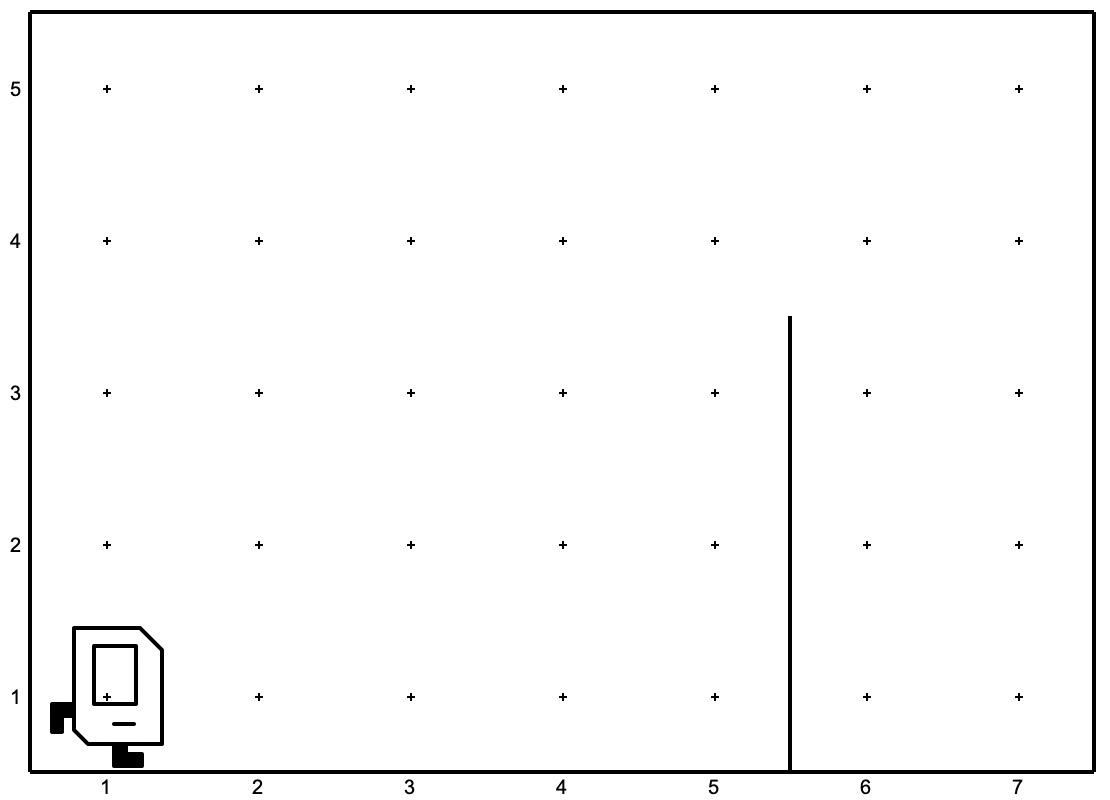
\includegraphics[scale=\figscale]{images/ch03/to_the_top/to_the_top_pre.jpg}
        \caption{မတိုင်မီ အခြေအနေ}   
        \label{fig:to_the_top_pre}
    \end{subfigure}
    \begin{subfigure}[t]{{\figpctw}\textwidth}
        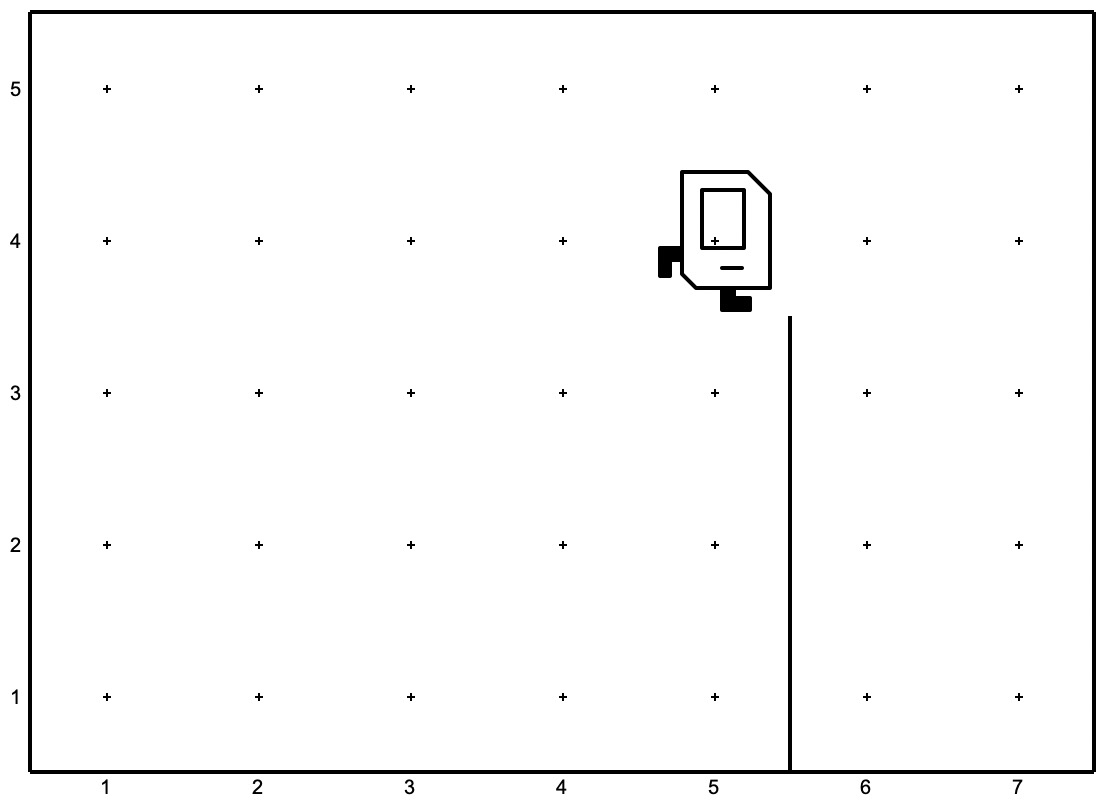
\includegraphics[scale=\figscale]{images/ch03/to_the_top/to_the_top_post.jpg}
        \caption{ပြီးနောက် အခြေအနေ} 
        \label{fig:to_the_top_post}   
    \end{subfigure}
    \caption{တိုင်ထိပ်သို့}
    \label{fig:to_the_top}
\end{figure}
%
တိုင်အောက်ခြေကိုသွားတာနဲ့ တိုင်ထိပ်တက်တာ အလုပ်နှစ်ခု ပါဝင်တယ်လို့ မြင်နိုင်တယ်။ ဒီအတွက် ဖန်ရှင်နှစ်ခု သတ်မှတ်ပေးပါမယ်။
%
\begin{py}
def go_to_pole():
    while front_is_clear():
        move()
\end{py}
%
%
\begin{py}
def ascend_pole():
    while right_is_blocked():
        move()
\end{py}
%
အထက်ပါ ဖန်ရှင်နှစ်ခုနဲ့ \fCode{go\_to\_top} ကို ဆက်လက် သတ်မှတ်ပါမယ်
%
\begin{py}
def go_to_top():
    go_to_pole()
    turn_left()
    ascend_pole()
    turn_right()
\end{py}
%
\fCode{go\_to\_pole} အပြီးမှာ ကားရဲလ်ဟာ တိုင်ခြေမှာ အရှေ့ဘက်မျက်နှာမူပြီး ရှိနေမှာပါ။ \fCode{ascend\_pole} က တိုင်ခြေမှာ ကားရဲလ် အပေါ်ဘက်ကို မျက်နှာမူတဲ့ အနေအထားကနေ စရပါမယ်။ \fCode{go\_to\_pole} ပြီးရင် \fCode{ascend\_pole} အတွက် အသင့်အနေအထားဖြစ်အောင် \fCode{turn\_left} လုပ်ပေးရပါမယ်။

ဖန်ရှင် စတင်မလုပ်ဆောင်မီ ကြိုတင်ရှိနေရမဲ့ အခြေအနေကို ပရီကွန်ဒီရှင်လို့ ပြောခဲ့ပါတယ်။ ဖန်ရှင် သတ်မှတ်တဲ့အခါ ပရီကွန်ဒီရှင်ကို တိတိကျကျ စဉ်းစားဖို့ လိုပါတယ်။ ဖန်ရှင်အသုံးပြုတဲ့အခါမှာလည်း သတ်မှတ်ထားတဲ့ ပရီကွန်ဒီရှင် အတိုင်းကိုက်ညီဖို့ လိုတယ်။ \fCode{ascend\_pole} ပရီကွန်ဒီးရှင်းဟာ တိုင်ခြေမှာ ကားရဲလ် အပေါ်ဘက်ကို မျက်နှာမူတဲ့ အနေအထား ဖြစ်ပါတယ်။ ပုံ \fRefNo{\ref{fig:mutp_pre_and_post}} (\fRefNo{\subref{fig:mutp_pre1}}) ကို ကြည့်ပါ။ %အကယ်၍ အဲဒီအတိုင်းမဟုတ်ရင် မက်သဒ်ကလည်း မှန်ကန်ကောင် လုပ်ဆောင်ပေးနိုင်ဖို့ မသေချာနိုင်ပါဘူး။

ဖန်ရှင် လုပ်ဆောင်အပြီးမှာ ရှိနေရမဲ့ အခြေအနေကို ပို့စ်ကွန်ဒီရှင်လို့ ဖော်ပြခဲ့တယ်။ ဖန်ရှင်တစ်ခုဟာ ပရီကွန်ဒီရှင်နဲ့ ကိုက်ညီတဲ့ အနေအထားကနေ စတင်ရင် ပို့စ်ကွန်ဒီရှင်နဲ့ ကိုက်ညီအောင်လုပ်ဆောင်ပေးပြီး အဆုံးသတ်ရမှာပါ။ ပုံ \fRefNo{\ref{fig:mutp_pre_and_post}} (\fRefNo{\subref{fig:mutp_post}}) မှာ \fCode{ascend\_pole} ပို့စ်ကွန်ဒီရှင်ကို တွေ့နိုင်ပါတယ်။
%
\begin{figure}[htb!]
    \hfuzz=100pt
    \newcommand{\figpctw}{0.52}
    \newcommand{\figscale}{0.165}
    \begin{subfigure}[t]{{\figpctw}\textwidth}
        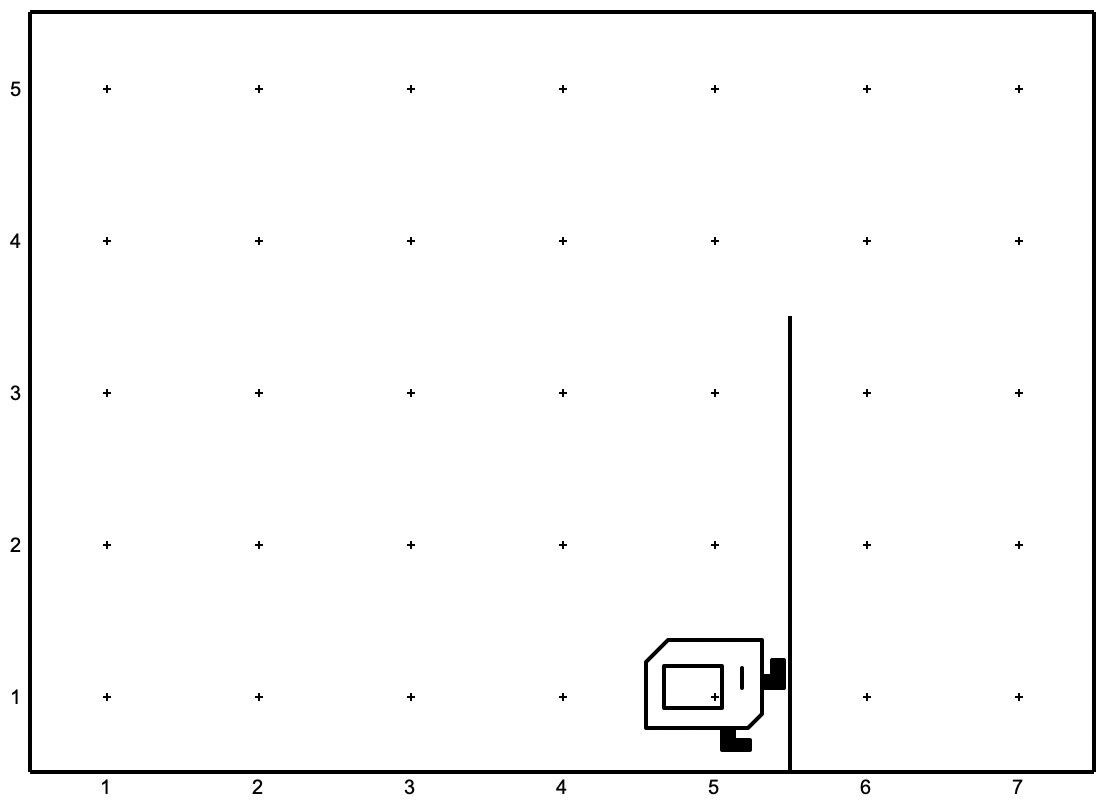
\includegraphics[scale=\figscale]{images/ch03/to_the_top/move_up_the_pole_pre1.jpg}
        \caption{}   
        \label{fig:mutp_pre1}
    \end{subfigure}
    \begin{subfigure}[t]{{\figpctw}\textwidth}
        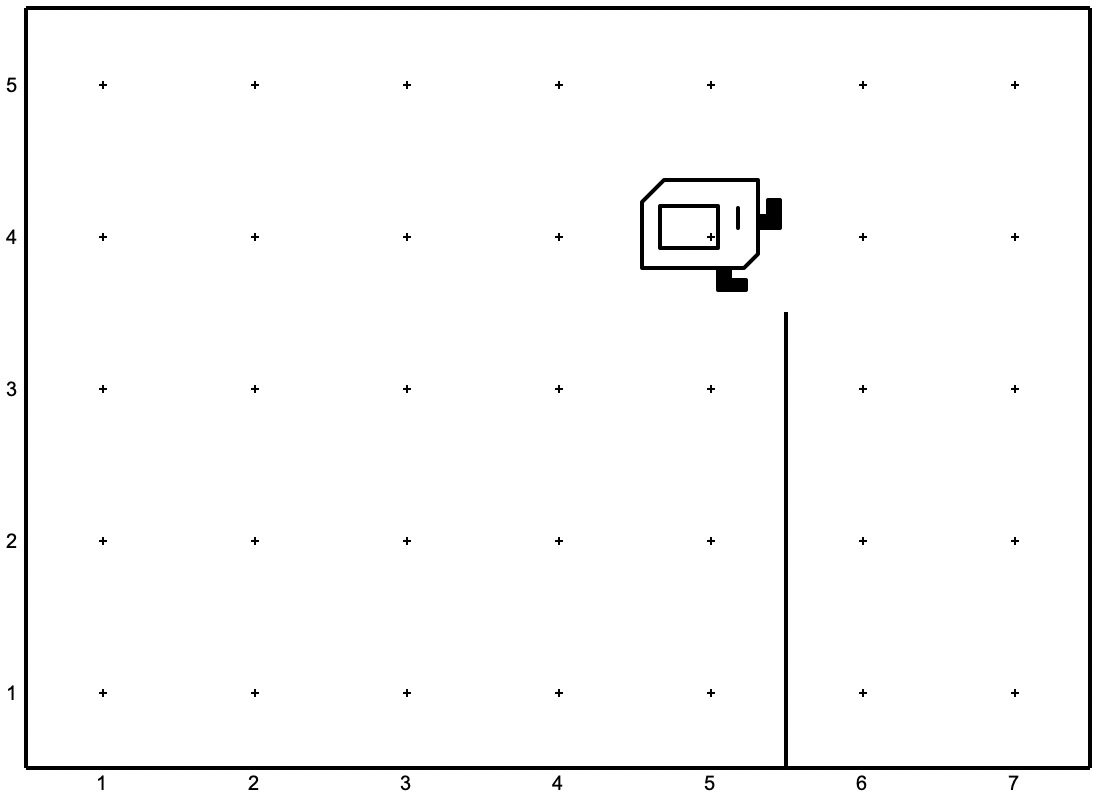
\includegraphics[scale=\figscale]{images/ch03/to_the_top/move_up_the_pole_post1.jpg}
        \caption{} 
        \label{fig:mutp_post}   
    \end{subfigure}
    \caption{\fCptCodeBf{ascend\_pole} ပရီကွန်ဒီးရှင်းနှင့် ပို့စ်ကွန်ဒီးရှင်း}
    \label{fig:mutp_pre_and_post}
\end{figure}


ဖန်ရှင် ပရီကွန်ဒီရှင် ပို့စ်ကွန်ဒီရှင်ကို သင့်တော်သလို သတ်မှတ်နိုင်ပါတယ်။ ပုံ (\fRefNo{\ref{fig:mutp_pre_and_post_v2}}) တွင် \fCode{ascend\_\allowbreak pole} အတွက် အခြား ရွေးချယ်နိုင်တဲ့ ပရီ နဲ့ ပို့စ် ကွန်ဒီရှင်ကို  ကြည့်ပါ။

\begin{figure}[tbh!]
    \hfuzz=100pt
    \newcommand{\figpctw}{0.52}
    \newcommand{\figscale}{0.165}
    \begin{subfigure}[t]{{\figpctw}\textwidth}
        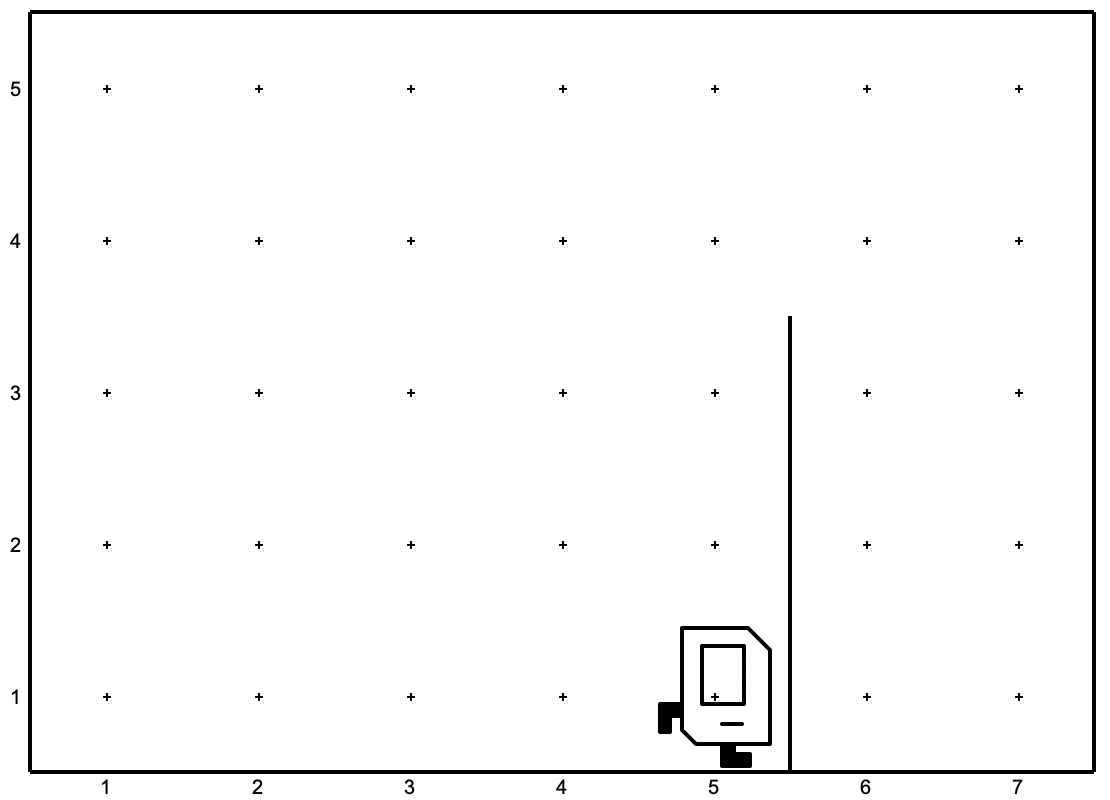
\includegraphics[scale=\figscale]{images/ch03/to_the_top/move_up_the_pole_pre_v2.jpg}
        \caption{}   
        \label{fig:mutp_pre_v2}
    \end{subfigure}
    \begin{subfigure}[t]{{\figpctw}\textwidth}
        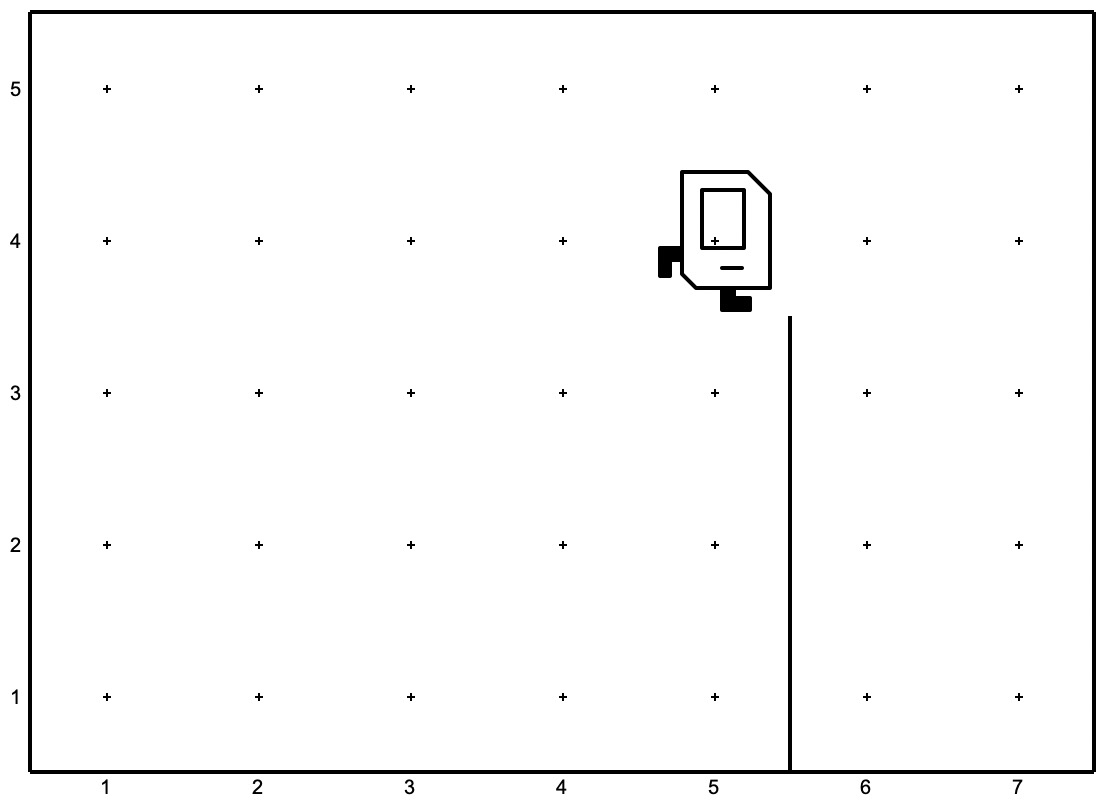
\includegraphics[scale=\figscale]{images/ch03/to_the_top/move_up_the_pole_post_v2.jpg}
        \caption{} 
        \label{fig:mutp_post_v2}   
    \end{subfigure}
    \caption{\fCptCodeBf{ascend\_pole} ပရီ နဲ့ ပို့စ် ကွန်ဒီရှင်}
    \label{fig:mutp_pre_and_post_v2}
\end{figure}

အထက်ပါ ပရီ နဲ့ ပို့စ် ကွန်ဒီရှင်အရ \fCode{ascend\_pole} ကို အခုလို 
%
\begin{py}
def ascend_pole():
    turn_left()
    while right_is_blocked():
        move()
    turn_right()
\end{py}
%
သတ်မှတ်ရမှာပါ။ \fCode{go\_to\_top} ကလည်း ဒီလို ဖြစ်သွားမယ်
%
\begin{py}
def go_to_top():
    go_to_pole()
    ascend_pole()
\end{py}
%

\section{ဖန်ရှင်များဖြင့် abstraction များ တည်ဆောက်ခြင်း}
အခန်း (\fRefNo{\ref{ch:ch02}}) စာမျက်နှာ (\fRefNo{\pageref{lst:repair_street}}) မှ လမ်းပြင်တဲ့ ပရိုဂရမ်မှာ ကွန်နာတစ်ခုဟာ ဘိပါလည်းမရှိ၊ အောက်ဘက်ကပ်လျက် နံရံလည်းမရှိရင်  ဘိပါတစ်ခု ချထားပေးရပါတယ်။ ဒီကိစ္စ ဆောင်ရွက်ပေးဖို့အတွက် ဖန်ရှင်တစ်ခု သတ်မှတ်နိုင်ပါတယ်။ 
%
\begin{figure}[htb!]
    {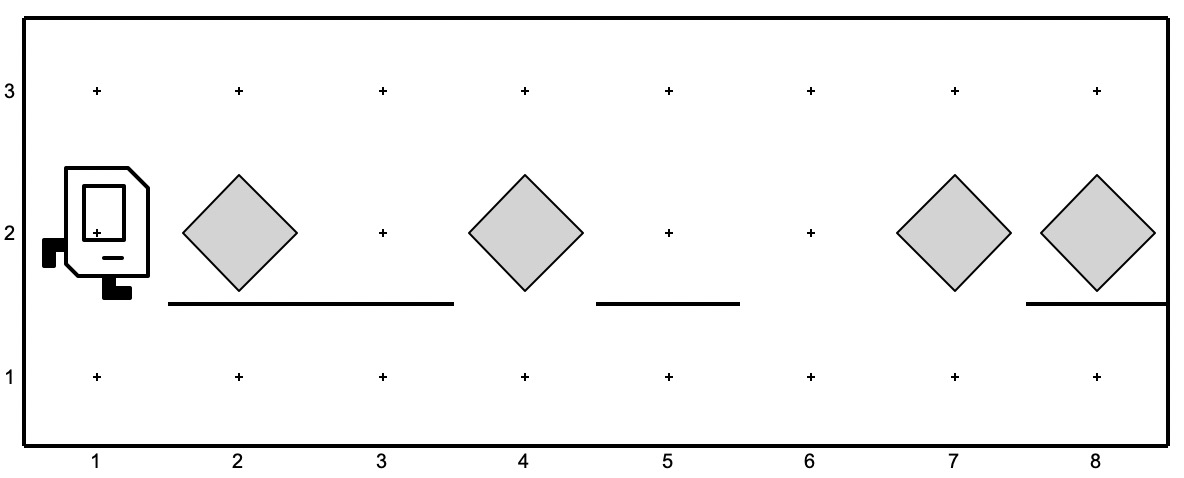
\includegraphics[width=0.5\linewidth]{images/ch02/st_repair/init.jpg}}
    \caption{}
\end{figure}
%
%
\begin{py}
def repair_corner():
    if right_is_clear():
        if no_beepers_present():
            put_beeper()
\end{py}
%
အခြေအနေနှစ်ခုစလုံး မှန်တော့မှ ဘိပါချပေးဖို့ \fEn{nested} \fCode{if}  သုံးထားတာက နားလည်ရ အတန်အသင့် ခက်ခဲနိုင်ပါတယ်။  ဒါပေမဲ့ \fCode{repair\_corner} ကို အသုံးပြုတဲ့အခါ ဘယ်လိုရေးထားလဲ စဉ်းစားစရာ မလိုပါဘူး။ ဘိပါလည်းမရှိ၊ ညာဘက် နံရံလည်းမရှိတဲ့ ကွန်နာမှာ ဘိပါချချင်ရင် \fCode{repair\_corner} ဖန်ရှင်နဲ့ လုပ်လို့ရတယ်ဆိုတာ သိထားရင် သုံးလို့ရပြီ။

ဖန်ရှင် သတ်မှတ်တဲ့အခါ ဆောင်ရွက်ပေးစေချင်တဲ့ ကိစ္စကို ‘ဘယ်လို လုပ်ရမှာလဲ’ အသေးစိတ် စဉ်းစားရမှာဖြစ်ပေမဲ့ အသုံးပြုတဲ့အခါမှာတော့ ဒီလိုအသေးစိတ်တွေကို ထပ်ပြီး စဉ်းစားဖို့ မလိုတော့ပါဘူး။ ဖန်ရှင် ‘ဘာလုပ်ပေးတာလဲ’ ကပဲ အရေးကြီးတယ်။ ‘ဘယ်လို’ တည်ဆောက်ထားလဲ သိစရာမလိုဘဲ ‘ဘာ’ လုပ်ပေးလဲ သိရုံနဲ့ အသုံးပြုလို့ရစေတာကို \fEn{abstraction} လုပ်တယ်လို့ခေါ်ပါတယ်။ \fEn{Abstraction} လုပ်ခြင်းအတွက် ဖန်ရှင်တွေဟာ အဓိက အကျဆုံး အခြေခံ အုတ်ချပ်တွေပါပဲ။ 


\fEn{Abstraction} လုပ်ထားလိုက်ခြင်းအားဖြင့် ရှုပ်ရှုပ်ထွေးထွေးတွေ ထပ်ခါထပ်ခါ ခေါင်းရှုပ်ခံ စဉ်းစားနေဖို့ မလိုအပ်တော့ဘဲ ကိစ္စတစ်ခုကို အလွယ်တကူ လုပ်ဆောင်လို့ရသွားတယ်။ ကုဒ်တွေဖတ်ရတာလည်း ပိုရှင်းပြီး နားလည်ရ လွယ်ကူသွားတယ်။ ဒါကြောင့် ပရိုဂရမ်တွေ တည်ဆောက်ရာမှာ \fEn{abstraction} လုပ်ခြင်းဟာ အရေးပါပါတယ်။ အရေးကြီးဆုံးလို့ ဆိုရင်လည်း မမှားဘူး။  ကြီးမားရှုပ်ထွေးတဲ့ ဆော့ဖ်ဝဲတွေကို လေ့လာကြည့်ရင်  \fEn{abstraction} ပေါင်းများစွာနဲ့ တစ်ဆင့်ပြီးတစ်ဆင့်၊ တစ်လွှာပြီးတစ်လွှာ တည်ဆောက်ထားတယ်ဆိုတာ တွေ့ရမှာပါ။

\fCode{repair\_corner} ဟာ အနိမ့်ဆုံးအလွှာက အခြေခံ \fEn{abstraction} တစ်ခု ဖြစ်တယ် ဆိုပါစို့။ ၎င်းကို အခြေခံပြီး တစ်ဆင့်ပိုမြင့်တဲ့ အလွှာအတွက် \fEn{abstraction} တွေကို တည်ဆောက်ယူနိုင်ပါတယ်။ ဥပမာ
%
\begin{py}
def repair_street():
    while front_is_clear():
        repair_corner()
    repair_corner()
\end{py}
%
ဒီအလွှာထက် နောက်ထပ် တစ်ဆင့်ပိုမြင့်တဲ့ \fEn{abstraction} တွေကိုလည်း ဆက်လက် တည်ဆောက်ယူနိုင်ပါတယ်။ ဥပမာ \fCode{repair\_world} ကို တည်ဆောက်ရာမှာ \fCode{repair\_street} ကို အခြေခံအစိတ်အပိုင်းအဖြစ် အသုံးပြုနိုင်ပါတယ်။ ဒီလို \fEn{abstraction} အလွှာတွေ အဆင့်ဆင့်နဲ့ ပရိုဂရမ် တည်ဆောက်နည်း တွေကို ဆက်လက်လေ့လာကြရပါမယ်။


\section{Bottom-up Programming}

ကြီးကျယ်ခမ်းနားတဲ့ အဆောက်အအုံကြီးတွေ၊ လျှို့ဝှက်ဆန်းကြယ်တဲ့ သဘာဝဖြစ်စဉ်တွေ၊ အံ့ဖွယ်သိပ္ပံနှင့် နည်းပညာ ဆန်းသစ်တီထွင်မှုတွေ စတဲ့အရာတွေအားလုံးဟာ ရိုးရှင်းတဲ့ အစိတ်အပိုင်းလေးတွေနဲ့ ဖွဲ့စည်းထားတာပါပဲ။ ဒါကြောင့် အရွယ်အစား ကြီးမား ရှုပ်ထွေးတဲ့ ပရိုဂရမ်တွေကိုလည်း ရိုးရှင်းတဲ့ အစိတ်အပိုင်းလေးတွေနဲ့ အခြေပြု ဖွဲ့စည်းတည်ဆောက်သင့်တယ်လို့ ယူဆမယ်ဆိုရင် ကျိုးကြောင်းဆီလျော်တယ်ပဲ ဆိုရမှာပါ။

ခက်ခဲရှုပ်ထွေးတဲ့ ကိစ္စတစ်ခုကို ဖြေရှင်းတဲ့အခါ အပိုင်းတွေခွဲပြီး တစ်ပိုင်းချင်းကို သီးခြားဖြေရှင်းလေ့ရှိတယ်။ အပိုင်းတွေခွဲလိုက်ခြင်းအားဖြင့် တစ်ပိုင်းစီဟာ မူလဖြေရှင်းရမဲ့ ကိစ္စလောက် မခက်ခဲတော့ပါဘူး။ အရွယ်အစားအားဖြင့်လည်း နဂိုထက် ငယ်သွားမယ်။ အပိုင်း တစ်ပိုင်းချင်းစီကို ဖြေရှင်းတဲ့အခါမှာလည်း အလားတူပဲ လုပ်ဆောင်နိုင်တယ်။ အပိုင်းတစ်ပိုင်းကို သူ့ထက်သေးငယ်တဲ့ အပိုင်းတွေအဖြစ် ထပ်မံခွဲထုတ်နိုင်ပါတယ်။ ဒီတိုင်း တစ်ဆင့်ပြီးတစ်ဆင့် လုပ်သွားမယ်ဆိုရင် နောက်ဆုံးမှာ အလွယ်တကူဖြေရှင်းလို့ရတဲ့ အစိတ်အပိုင်းလေးတွေ ဖြစ်သွားရမှာပါပဲ။ \fEnEmp{Bottom-up programming} ဆိုတာကတော့ ပရိုဂရမ်ရေးပြီး ကိစ္စတစ်ခုကို ဖြေရှင်းရာမှာ ရိုးရှင်းသထက်ရိုးရှင်း၊ သေးငယ်သထက်သေးငယ်တဲ့ အပိုင်းလေးတွေဖြစ်လာအောင် အဆင့်ဆင့်ပိုင်းခွဲပြီး အောက်ခြေအရိုးရှင်းဆုံးအလွှာကနေ အပေါ်ကိုတစ်ဆင့်ချင်းတက် ဖြေရှင်းတဲ့နည်း ဖြစ်တယ်။ လေ့လာကြည့်ကြရအောင်။

ပုံ (\fRefNo{\ref{fig:hurdle_jumping_init}}) ကမ္ဘာမှာ ကားရဲလ် တန်းကျော်ပြေးပြိုင်ရပါမယ်။ ထောင်လိုက်နံရံတွေကို တန်းတွေလို့ယူဆပါ။ တန်းတွေဟာ အနိမ့်အမြင့် အမျိုးမျိုးဖြစ်နိုင်ပါတယ်။ ကမ္ဘာရဲ့ အပေါ်ဘက် နံရံကို ထိတဲ့အထိတော့ မြင့်လို့မရပါဘူး။ ဒါမှ တန်းကိုကျော်ပြီး အခြားဘက်ကို သွားလို့ရမှာပါ။ \((1, 1)\) ကွန်နာကနေ တာစထွက်မှာဖြစ်ပြီး \((14, 1)\) မှာ ပန်းဝင်ရမှာပါ။
%
\begin{figure}[htb!]
    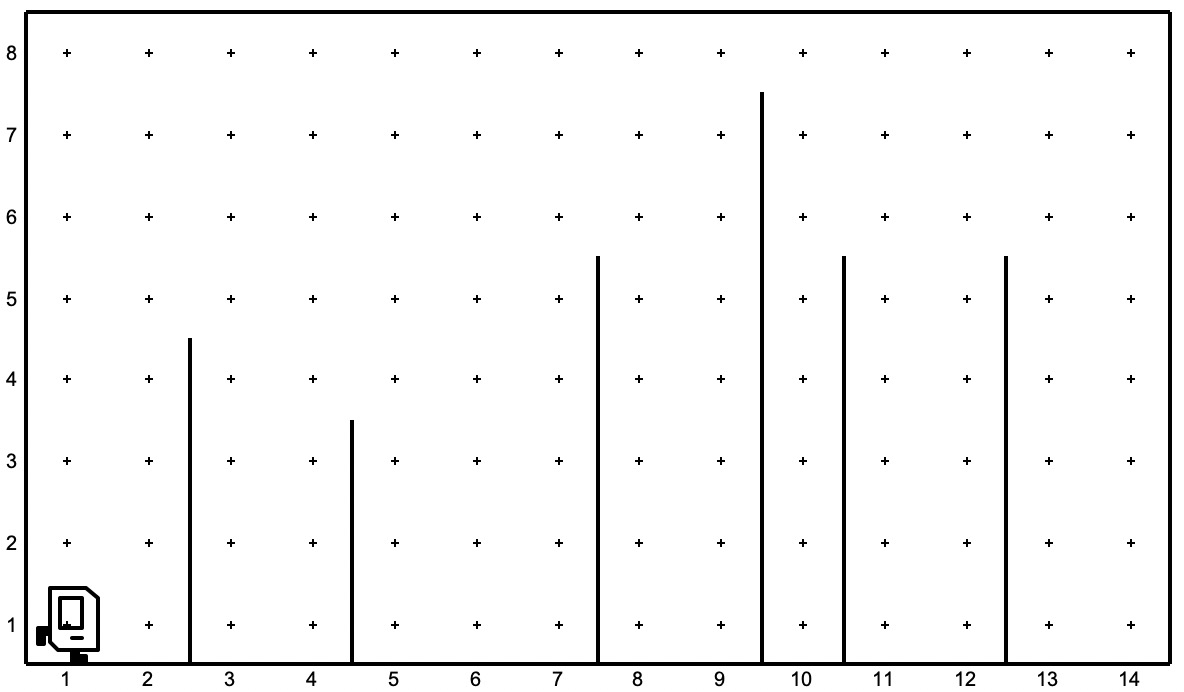
\includegraphics[width=4.5in]{images/ch03/hurdle_jumping/init_w1.jpg}
    \caption{}
    \label{fig:hurdle_jumping_init}
\end{figure}
%

တန်းကျော်ပြေးတဲ့ ကိစ္စမှာ ပါဝင်တဲ့ အပိုင်းတစ်ခုက တန်းတစ်ခုကျော်တာ။ တန်းတစ်ခု ကျော်တာကို ထပ်ခွဲကြည့်ရင် အပေါ်တက်တာနဲ့ အောက်ဆင်းတာ နှစ်ပိုင်းရှိမယ်။ အခုလို နဂိုမူလကိစ္စတစ်ခုကနေ တစ်ဆင့်ထက်တစ်ဆင့် ပိုသေးငယ်တဲ့ အပိုင်းလေးတွေဖြစ်လာအောင် ခွဲထုတ်တာကို \fEnEmp{problem decomposition} လုပ်တယ်လို ခေါ်ပါတယ်။ 

\fEn{Bottom-up programming} နည်းနဲ့ ပရိုဂရမ်ရေးတဲ့အခါ \fEn{problem decomposition} အရင်ဦးဆုံး  လုပ်ရတယ်။ ပြီးရင် အောက်ဆုံးအလွှာမှ အသေးဆုံးအပိုင်းလေးတွေကနေ စတင်ဖြေရှင်းတယ်။ ပြီးတဲ့အခါ အဲဒီ အသေးဆုံး အပိုင်းလေးတွေကို အခြေခံအစိတ်အပိုင်းအဖြစ် အသုံးပြုပြီး  အောက်ဆုံးအလွှာထက် တစ်ဆင့်မြင့်တဲ့ အပေါ်အလွှာက အပိုင်းတွေကို ဆက်လက်ဖြေရှင်းတယ်။ ဒီအလွှာက အပိုင်းတွေကို  အခြေခံအစိတ်အပိုင်းအဖြစ် အသုံးပြုပြီး နောက်ထပ်တစ်ဆင့် ပိုမြင့်တဲ့အလွှာက အပိုင်းတွေကို ဆက်လက်ဖြေရှင်းမှာဖြစ်တယ်။ ဒီလိုမျိုး အောက်ကနေ အပေါ်ကို တစ်လွှာပြီးတစ်လွှာ တက်သွားပြီး ဖြေရှင်းတဲ့ နည်းစနစ်ဟာ \fEn{bottom-up programming} ပါပဲ။ 

တန်းကျော်ပြေးပွဲမှာ \fEn{Problem Decomposition} လုပ်ထားတာကို တစ်လွှာချင်း ခွဲကြည့်မယ်ဆိုရင် အခုလိုတွေ့ရမှာ ဖြစ်ပါတယ်။
%
\begin{itemize}
  \item တန်းကျော်ပြေးပြိုင်ပွဲဝင်ခြင်း
  \begin{itemize}
    \item တန်းတစ်ခုကျော်ခြင်း
    \begin{itemize}
      \item အပေါ်တက်ခြင်း
      \item အောက်ဆင်းခြင်း
    \end{itemize}
  \end{itemize} 
\end{itemize}
%
\fEn{Bottom-up} နည်းအရ အောက်ဆုံးအလွှာ အပေါ်တက်၊ အောက်ဆင်း ကိစ္စကို ပထမဆုံး ဖြေရှင်းပါမယ်။ အပိုင်းတစ်ခုအတွက် ဖန်ရှင်တစ်ခု သတ်မှတ်ရပါမယ်။

%
\begin{py}
def ascend():
    ß\PYG{l+s+sd}{\PYGZdq{}\PYGZdq{}\PYGZdq{}}ß
    ß\PYG{l+s+sd}{\fMM{တန်းနဲ့လွတ်တဲ့အထိ အပေါ်သို့ တက်သည်}}ß
    ß\PYG{l+s+sd}{\fEnEmp{Precondition:} \fMM{တန်းဘယ်ဘက် ခြေရင်းမှာ အရှေ့ဘက်မျက်နှာမူပြီး ရှိနေ}}ß
    ß\PYG{l+s+sd}{\fEnEmp{Postcondition:} \fMM{တန်းထိပ်အပေါ် ဘယ်ဘက်ကွန်နာမှာ အရှေ့ဘက်မျက်နှာမူပြီး ရှိနေ}}ß
    ß\PYG{l+s+sd}{\PYGZdq{}\PYGZdq{}\PYGZdq{}}ß
    turn_left()
    while right_is_blocked():
        move()
    turn_right()
\end{py}
%
%
\begin{py}
def descend():
    ß\PYG{l+s+sd}{\PYGZdq{}\PYGZdq{}\PYGZdq{}}ß
    ß\PYG{l+s+sd}{\fMM{တန်းအောက်သို့ ပြန်ဆင်းသည်}}ß
    ß\PYG{l+s+sd}{\fEnEmp{Precondition:} \fMM{တန်းထိပ်အပေါ် ညာဘက်ကွန်နာမှာ အရှေ့ဘက်မျက်နှာမူပြီး ရှိနေ}}ß
    ß\PYG{l+s+sd}{\fEnEmp{Postcondition:} \fMM{တန်းညာဘက် ခြေရင်းမှာ အရှေ့ဘက်မျက်နှာမူပြီး ရှိနေ}}ß
    ß\PYG{l+s+sd}{\PYGZdq{}\PYGZdq{}\PYGZdq{}}ß
    turn_right()
    while front_is_clear():
        move()
    turn_left()
\end{py}
%

အထက်ပါ ဖန်ရှင်နှစ်ခုကို အသုံးပြုပြီး အပေါ်တစ်ဆင့် ပိုမြင့်တဲ့ အလွှာက တန်းတစ်ခုကျော်တာကို ဆက်လက်ဖြေရှင်းရပါမယ်။ \fCode{ascend} နဲ့ \fCode{descend} ပရီနဲ့ ပို့စ် ကွန်ဒီရှင်တွေအရ \fCode{move} လုပ်ပေးဖို့လိုပါတယ်။
%
\begin{py}
def jump_over_hurdle():
    ß\PYG{l+s+sd}{\PYGZdq{}\PYGZdq{}\PYGZdq{}}ß
    ß\PYG{l+s+sd}{\fMM{တန်းတစ်ခုကို ကျော်သည်}}ß
    ß\PYG{l+s+sd}{\fEnEmp{Precondition:} \fMM{တန်းဘယ်ဘက် ခြေရင်းမှာ အရှေ့ဘက်မျက်နှာမူပြီး ရှိနေ}}ß
    ß\PYG{l+s+sd}{\fEnEmp{Postcondition:} \fMM{တန်းညာဘက် ခြေရင်းမှာ အရှေ့ဘက်မျက်နှာမူပြီး ရှိနေ}}ß
    ß\PYG{l+s+sd}{\PYGZdq{}\PYGZdq{}\PYGZdq{}}ß
    ascend()
    move()
    descend()
\end{py}
%

ဒီဖန်ရှင်နဲ့ နောက်တစ်ဆင့်ကို ဆက်လက်တည်ဆောက်ရပါမယ်။ ရှေ့မှာရှင်းနေလျှင် ရှေ့တိုးမယ်၊ မရှင်းလျှင် တန်းကိုကျော်ရမယ်။ ပန်းဝင်ဖို့အတွက်ဆိုလျှင် ဒီအလုပ်ကို ဆယ့်သုံးခါလုပ်ပေးရုံပါပဲ။
%
\begin{py}
def compete_hurdle_race():
    ß\PYG{l+s+sd}{\PYGZdq{}\PYGZdq{}\PYGZdq{}}ß
    ß\PYG{l+s+sd}{\fMM{တန်းကျော်ပြေးပြိုင်ပွဲ ပန်းဝင်သည်ထိ ယှဉ်ပြိုင်သည်}}ß
    ß\PYG{l+s+sd}{\fEnEmp{Precondition:} \fMM{(၁,၁) ကွန်နာတွင် အရှေ့ဘက်မျက်နှာမူနေ}}ß
    ß\PYG{l+s+sd}{\fEnEmp{Postcondition:} \fMM{(၁၄,၁) ကွန်နာတွင် အရှေ့ဘက်မျက်နှာမူနေ}}ß
    ß\PYG{l+s+sd}{\PYGZdq{}\PYGZdq{}\PYGZdq{}}ß
    for i in range(13):
        if front_is_clear():
            move()
        else:
            jump_over_hurdle()
\end{py}
%

ပရိုဂရမ် အစအဆုံးကို လေ့လာကြည့်ပါ။ ဖန်ရှင်တစ်ခုချင်း ပရီနဲ့ ပို့စ် ကွန်ဒီရှင်တွေကို တိတိကျကျ မြင်အောင် ဂရုစိုက်ကြည့်ဖို့လည်း အရေးကြီးတယ်။ ဖန်ရှင် \fEn{docstring} မှာ ၎င်းဖန်ရှင် ပရီနဲ့ ပို့စ် ကွန်ဒီရှင်ကို တိတိကျကျ ဖော်ပြထားတာဟာ အလေ့အထကောင်း တစ်ခုပါ။ ဖန်ရှင်တိုင်းမှာ ပါသင့်တယ်။

%
\begin{py}
# File: hurdle_jumping.py
from stanfordkarel import *


def main():
    """Hurdle Jumping Program"""
    compete_hurdle_race()


def ascend():
    ß\PYG{l+s+sd}{\PYGZdq{}\PYGZdq{}\PYGZdq{}}ß
    ß\PYG{l+s+sd}{\fMM{တန်းနဲ့လွတ်တဲ့အထိ အပေါ်သို့ တက်သည်}}ß
    ß\PYG{l+s+sd}{\fEnEmp{Precondition:} \fMM{တန်းဘယ်ဘက် ခြေရင်းမှာ အရှေ့ဘက်မျက်နှာမူပြီး ရှိနေ}}ß
    ß\PYG{l+s+sd}{\fEnEmp{Postcondition:} \fMM{တန်းထိပ်အပေါ် ဘယ်ဘက်ကွန်နာမှာ အရှေ့ဘက်မျက်နှာမူပြီး ရှိနေ}}ß
    ß\PYG{l+s+sd}{\PYGZdq{}\PYGZdq{}\PYGZdq{}}ß
    turn_left()
    while right_is_blocked():
        move()
    turn_right()


def descend():
    ß\PYG{l+s+sd}{\PYGZdq{}\PYGZdq{}\PYGZdq{}}ß
    ß\PYG{l+s+sd}{\fMM{တန်းအောက်သို့ ပြန်ဆင်းသည်}}ß
    ß\PYG{l+s+sd}{\fEnEmp{Precondition:} \fMM{တန်းထိပ်အပေါ် ညာဘက်ကွန်နာမှာ အရှေ့ဘက်မျက်နှာမူပြီး ရှိနေ}}ß
    ß\PYG{l+s+sd}{\fEnEmp{Postcondition:} \fMM{တန်းညာဘက် ခြေရင်းမှာ အရှေ့ဘက်မျက်နှာမူပြီး ရှိနေ}}ß
    ß\PYG{l+s+sd}{\PYGZdq{}\PYGZdq{}\PYGZdq{}}ß
    turn_right()
    while front_is_clear():
        move()
    turn_left()


def jump_over_hurdle():
    ß\PYG{l+s+sd}{\PYGZdq{}\PYGZdq{}\PYGZdq{}}ß
    ß\PYG{l+s+sd}{\fMM{တန်းတစ်ခုကို ကျော်သည်}}ß
    ß\PYG{l+s+sd}{\fEnEmp{Precondition:} \fMM{တန်းဘယ်ဘက် ခြေရင်းမှာ အရှေ့ဘက်မျက်နှာမူပြီး ရှိနေ}}ß
    ß\PYG{l+s+sd}{\fEnEmp{Postcondition:} \fMM{တန်းညာဘက် ခြေရင်းမှာ အရှေ့ဘက်မျက်နှာမူပြီး ရှိနေ}}ß
    ß\PYG{l+s+sd}{\PYGZdq{}\PYGZdq{}\PYGZdq{}}ß
    ascend()
    move()
    descend()


def compete_hurdle_race():
    ß\PYG{l+s+sd}{\PYGZdq{}\PYGZdq{}\PYGZdq{}}ß
    ß\PYG{l+s+sd}{\fMM{တန်းကျော်ပြေးပြိုင်ပွဲ ပန်းဝင်သည်ထိ ယှဉ်ပြိုင်သည်}}ß
    ß\PYG{l+s+sd}{\fEnEmp{Precondition:} \fMM{(၁,၁) ကွန်နာတွင် အရှေ့ဘက်မျက်နှာမူနေ}}ß
    ß\PYG{l+s+sd}{\fEnEmp{Postcondition:} \fMM{(၁၄,၁) ကွန်နာတွင် အရှေ့ဘက်မျက်နှာမူနေ}}ß
    ß\PYG{l+s+sd}{\PYGZdq{}\PYGZdq{}\PYGZdq{}}ß
    for i in range(13):
        if front_is_clear():
            move()
        else:
            jump_over_hurdle()


def turn_right():
    for i in range(3):
        turn_left()


if __name__ == "__main__":
    run_karel_program("hurdle_jumping")

\end{py}
%


\subsection*{အမှိုက်သိမ်းတဲ့ ကားရဲလ်}
အခုတစ်ခါမှာ ကားရဲလ်က အမှိုက်တွေရှင်းပေးရပါမယ်။ ပုံ (\fRefNo{\ref{fig:stw}}) နမူနာ ကမ္ဘာမှာ ကြုံရာကျပန်း \fEn{(random)} ပြန့်ကျဲနေတဲ့ ဘိပါတွေကို အမှိုက်လို့ ယူဆပါ။  ကမ္ဘာအရွယ်အစား အမျိုးမျိုးအတွက် အမှိုက်ရှင်းပေးတဲ့ ပရိုဂရမ်တစ်ခု ရေးပေးရမှာပါ။
\begin{figure}[htb!]
    {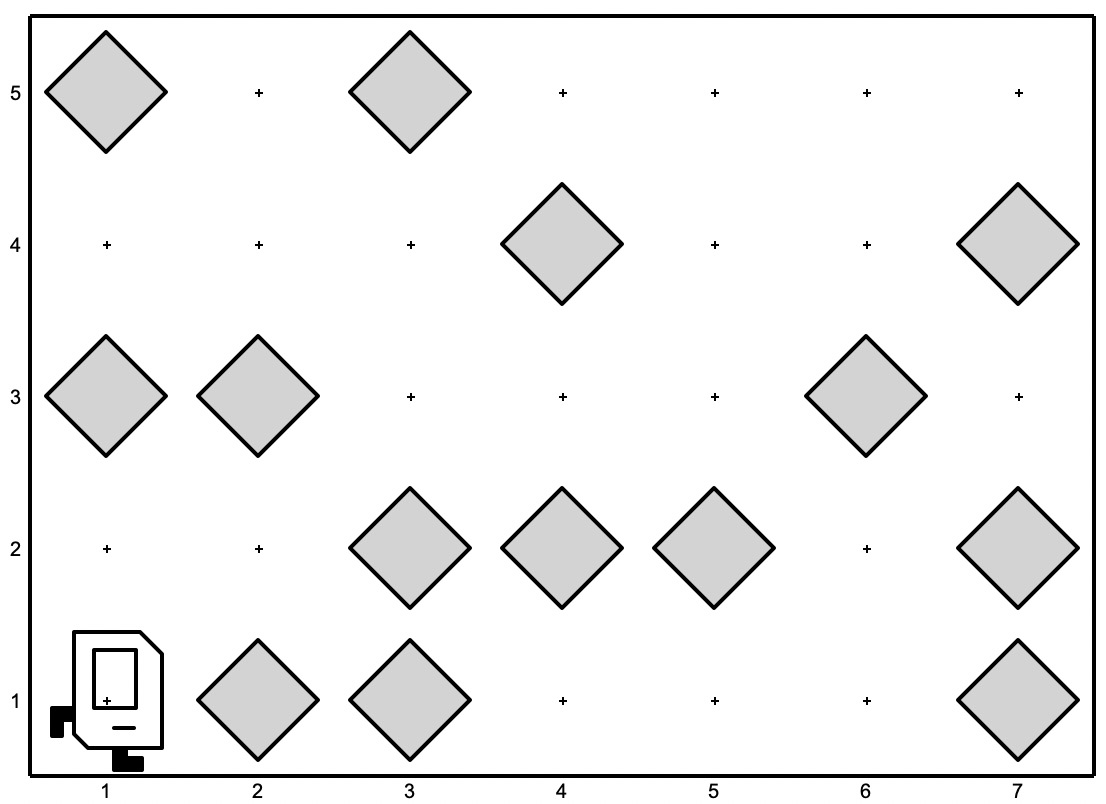
\includegraphics[width=.5\linewidth]{images/ch03/clean_the_world/init_w1.jpg}}
\caption{}
\label{fig:stw}
\end{figure}

ဒီကိစ္စကို ဖြေရှင်းဖို့က နည်းလမ်းတစ်ခုတည်း ရှိတာ မဟုတ်ပါဘူး။ နည်းလမ်းတစ်ခုက ဒီလိုပါ။ (၁) လမ်းကနေ စပြီး ရှင်းတယ် $\big\llbracket$စာမျက်နှာ \fRefNo{\pageref{fig:stw_alg1}} ပုံ (\fRefNo{\ref{fig:stw_alg1}}) (က) နှင့် (ခ) တွင် ကြည့်ပါ$\big\rrbracket$။ ပြီးရင် မြောက်ဘက် လှည့်ထားမယ် $\big\llbracket$ပုံ (\fRefNo{\ref{fig:stw_alg1}}) (ဂ)$\big\rrbracket$။ ရှင်းနေသေးတယ်ဆိုရင် ဒုတိယလမ်းကို တက်၊ အနောက်ဘက် မျက်နှာမူထားမယ် $\big\llbracket$ပုံ (\fRefNo{\ref{fig:stw_alg1}}) (ဃ)$\big\rrbracket$။ ဒုတိယလမ်းကို ဆက်ရှင်းပြီးတော့လည်း မြောက်ဘက်ကိုပဲ မျက်နှာမူထားပါမယ် $\big\llbracket$ပုံ (\fRefNo{\ref{fig:stw_alg1}}) (င)၊ (စ)$\big\rrbracket$။ ရှင်းနေသေးရင် တတိယလမ်းကို ကူး၊ အရှေ့ဘက်မျက်နှာ မူထားမယ် $\big\llbracket$ပုံ (\fRefNo{\ref{fig:stw_alg1}}) (ဆ)$\big\rrbracket$။ ဒီအတိုင်း တစ်လမ်းပြီးတစ်လမ်း ရှင်းသွားမှာဖြစ်တယ်။ လမ်းတစ်လမ်းရှင်းပြီး မြောက်ဘက်မျက်နှာမူလို့ ပိတ်နေရင် နောက်ထပ် လမ်းမရှိတော့ဘူး။ လမ်းအားလုံး ရှင်းပြီးသွားပြီ။ စာမျက်နှာ \fRefNo{\pageref{fig:stw_alg1_last_st}} ပုံ (\fRefNo{\ref{fig:stw_alg1_last_st}}) (က)၊ (ခ)၊ (ဂ) တို့ကို ကြည့်ပါ။ \fEn{Problem decomposition} လုပ်ကြည့်ရင် အောက်ပါအတိုင်း တွေ့နိုင်ပါတယ်။ 

%
\begin{figure}[htb!]
    \hfuzz=100pt
    \newcommand{\figpctw}{0.52}
    \newcommand{\figscale}{0.165}
    \begin{subfigure}[t]{{\figpctw}\textwidth}
        %\adjincludegraphics[width=2.5in,trim={0 0 0 {.55\height}}, clip, left]{ch03/SweepTheStreets/init_w1.jpg}
        \adjincludegraphics[scale=\figscale, trim={0 3pt 0 10cm}, clip, left]{images/ch03/clean_the_world/alg1/stp1a.jpg}
        \caption{}
        \label{fig:fst_bef}
    \end{subfigure}
    \begin{subfigure}[t]{{\figpctw}\textwidth}
        \adjincludegraphics[scale=\figscale, trim={0 3pt 0 10cm}, clip, left]{images/ch03/clean_the_world/alg1/stp1b.jpg}
        \caption{}
        \label{fig:fst_aft}
    \end{subfigure}

    \begin{subfigure}[t]{{\figpctw}\textwidth}
        \adjincludegraphics[scale=\figscale, trim={0 3pt 0 10cm}, clip, left]{images/ch03/clean_the_world/alg1/stp2.jpg}
        \caption{}
        \label{fig:fst_tn}
    \end{subfigure}
    \begin{subfigure}[t]{{\figpctw}\textwidth}
        \adjincludegraphics[scale=\figscale, trim={0 3pt 0 10cm}, clip, left]{images/ch03/clean_the_world/alg1/stp3a.jpg}
        \caption{}
        \label{fig:xyz4}
    \end{subfigure}
    \begin{subfigure}[t]{{\figpctw}\textwidth}
        \adjincludegraphics[scale=\figscale, trim={0 3pt 0 10cm}, clip, left]{images/ch03/clean_the_world/alg1/stp3b.jpg}
        \caption{}
        \label{fig:xyz5}
    \end{subfigure}
    \begin{subfigure}[t]{{\figpctw}\textwidth}
        \adjincludegraphics[scale=\figscale, trim={0 3pt 0 10cm}, clip, left]{images/ch03/clean_the_world/alg1/stp4.jpg}
        \caption{}
        \label{fig:xyz6}
    \end{subfigure}
    \begin{subfigure}[t]{{\figpctw}\textwidth}
        \adjincludegraphics[scale=\figscale, trim={0 3pt 0 10cm}, clip, left]{images/ch03/clean_the_world/alg1/stp5a.jpg}
        \caption{}
        \label{fig:xyz7}
    \end{subfigure}
    \begin{subfigure}[t]{{\figpctw}\textwidth}
        \adjincludegraphics[scale=\figscale, trim={0 3pt 0 10cm}, clip, left]{images/ch03/clean_the_world/alg1/stp5b.jpg}
        \caption{}
        \label{fig:xyz8}
    \end{subfigure}
    \caption{}
    \label{fig:stw_alg1}
\end{figure}
%

%
\begin{figure}[htb!]
    %\adjincludegraphics[width=2.5in,trim={0 0 0 {.55\height}}, clip, left]{images/}
    \hfuzz=100pt
    \newcommand{\figpctw}{0.52}
    \newcommand{\figscale}{0.165}
    \begin{subfigure}[t]{{\figpctw}\textwidth}
        \adjincludegraphics[scale=\figscale, trim={0 15cm 0 0}, clip, left]{images/ch03/clean_the_world/alg1/stp6a.jpg}
        \caption{}
    \end{subfigure}
    \begin{subfigure}[t]{{\figpctw}\textwidth}
        \adjincludegraphics[scale=\figscale, trim={0 15cm 0 0}, clip, left]{images/ch03/clean_the_world/alg1/stp6b.jpg}
        \caption{}
    \end{subfigure}
    \begin{subfigure}[t]{{\figpctw}\textwidth}
        \adjincludegraphics[scale=\figscale, trim={0 15cm 0 0}, clip, left]{images/ch03/clean_the_world/alg1/stp7.jpg}
        \caption{}
    \end{subfigure}
    \caption{}
    \label{fig:stw_alg1_last_st}
\end{figure}
%

%
\begin{itemize} \label{fig:btmup_pd}
    \item ကမ္ဘာတစ်ခုလုံး အမှိုက်တွေရှင်း \fEn{(clean world)}
    %
    \begin{itemize}
        \item လမ်းတစ်လမ်း အမှိုက်ရှင်း  \fEn{(clean street)}     
        %
        \begin{itemize}
            \item ကွန်နာတစ်ခု အမှိုက်ရှင်း \fEn{(clean corner)}
        \end{itemize}
        %
        \item မြောက်ဘက်လှည့် \fEn{(turn north)}
        \item လမ်းပြောင်း/နောက်တစ်လမ်းကူး \fEn{(change street)}
    \end{itemize}
    %
\end{itemize}
%

လမ်းတစ်လမ်း ရှင်းတဲ့ ကိစ္စကို ထပ်ခွဲကြည့်ရင် ကွန်နာတစ်ခုရှင်းတာကို တွေ့ရမှာပါ။ \fEn{Bottom-up} နည်းအရ အောက်ဆုံးအလွှာက ကွန်နာတစ်ခု အမှိုက်ရှင်းတဲ့ ကိစ္စအတွက် ဖန်ရှင်ကို ပထမဆုံး သတ်မှတ်ရပါမယ်။
%
\begin{py}
def clean_corner():
    ß\PYG{l+s+sd}{\PYGZdq{}\PYGZdq{}\PYGZdq{}}ß
    ß\PYG{l+s+sd}{\fMM{ကွန်နာတစ်ခုမှာ ဘိပါရှင်းပေးသည်}}ß
    ß\PYG{l+s+sd}{\fEnEmp{Precondition:} \fMM{ကွန်နာတစ်ခုမှာ ကားရဲလ် ရှိနေမယ်။ အများဆုံး ဘိပါတစ်ခု ရှိနိုင်တယ်။}}ß
    ß\PYG{l+s+sd}{\fEnEmp{Postcondition:} \fMM{ဘိပါ မရှိတဲ့ ကွန်နာဖြစ်ရမယ်}}ß
    ß\PYG{l+s+sd}{\PYGZdq{}\PYGZdq{}\PYGZdq{}}ß
    if beepers_present():
        pick_beeper()
\end{py}
%
\fCode{clean\_corner} နဲ့ လမ်းတစ်လမ်းရှင်းတဲ့ ဖန်ရှင် သတ်မှတ်ပါမယ်။
%
\begin{py}
def clean_street():
    ß\PYG{l+s+sd}{\PYGZdq{}\PYGZdq{}\PYGZdq{}}ß
    ß\PYG{l+s+sd}{\fMM{လမ်းတလျှောက် ဘိပါအားလုံးရှင်းပေးသည်}}ß
    ß\PYG{l+s+sd}{\fEnEmp{Precondition:} \fMM{လမ်းအစွန်းတစ်ဖက်မှာ အခြားဘက်စွန်းကို မျက်နှာမူ၍ ရှိမယ်}}ß
    ß\PYG{l+s+sd}{\fEnEmp{Postcondition:} \fMM{လမ်းပေါ်ဘိပါအားလုံး ရှင်းပြီး အခြားဘက်စွန်း ရောက်နေမယ်}}ß
    ß\PYG{l+s+sd}{\PYGZdq{}\PYGZdq{}\PYGZdq{}}ß
    while front_is_clear():
        clean_corner()
        move()
    clean_corner()
\end{py}
%
မြောက်ဘက်လှည့်တဲ့ ဖန်ရှင်
%
\begin{py}
def turn_north():
    while not_facing_north():
        turn_left()
\end{py}
%
\fCode{while} \fEn{loop} နဲ့ မြောက်ဘက်ကို မျက်နှာမူ မနေသ၍ ဘယ်ဘက်လှည့်ခိုင်းထားတာ သတိထားကြည့်ပါ။ မြောက်ဘက် မျက်နှာမူနေတဲ့ အနေအထားမှာ ရပ်သွားမှာ ဖြစ်တယ်။

လမ်းတစ်လမ်းရှင်းပြီး နောက်တစ်လမ်းကူးတဲ့ ဖန်ရှင်
%
\begin{py}
def change_street():
    ß\PYG{l+s+sd}{\PYGZdq{}\PYGZdq{}\PYGZdq{}}ß
    ß\PYG{l+s+sd}{\fMM{လမ်းတစ်လမ်း၏ အစွန်းတစ်ဖက်မှာ အပေါ်လမ်းသို့ ကူးသည်}}ß
    ß\PYG{l+s+sd}{\fEnEmp{Precondition:} \fMM{လမ်းအစွန်းတစ်ဖက်မှာ ကပ်လျက် နံရံကို မျက်နှာမူ၍ ရှိမယ်}}ß
    ß\PYG{l+s+sd}{\fEnEmp{Postcondition:} \fMM{အပေါ်တစ်လမ်းကူးပြီး အခြားဘက်စွန်းကို မျက်နှာမူ၍ ရှိမယ်}}ß
    ß\PYG{l+s+sd}{\PYGZdq{}\PYGZdq{}\PYGZdq{}}ß
    move()
    if right_is_blocked():
        turn_left()
    else:
        turn_right()
\end{py}
%
တစ်လမ်းချင်း အမှိုက်အကုန် ရှင်းတဲ့ ဖန်ရှင်ကို သတ်မှတ်လို့ ရပါပြီ
%
\begin{py}
def clean_world():
    ß\PYG{l+s+sd}{\PYGZdq{}\PYGZdq{}\PYGZdq{}}ß
    ß\PYG{l+s+sd}{\fMM{လမ်းအားလုံးမှ ဘိပါတွေ ရှင်းပေး}}ß
    ß\PYG{l+s+sd}{\fEnEmp{Precondition:} \fMM{(၁,၁) ကွန်နာမှာ အရှေ့ဘက် မျက်နှာမူ၍ ရှိနေမယ်}}ß
    ß\PYG{l+s+sd}{\fEnEmp{Postcondition:} \fMM{လမ်းအားလုံး အမှိုက်ရှင်းပြီး ဖြစ်မယ်}}ß
    ß\PYG{l+s+sd}{\PYGZdq{}\PYGZdq{}\PYGZdq{}}ß
    clean_street()
    turn_north()
    while front_is_clear():
        change_street()
        clean_street()
        turn_north()
\end{py}
%
ပရိုဂရမ် အစအဆုံး ဆက်လက်လေ့လာကြည့်ပါ။ (ပရီနဲ့ ပို့စ် ကွန်ဒီရှင်တွေကို ချန်ထားတယ်။ နေရာသက်သာအောင်ပါ။ အပြည့်အစုံ ရေးတဲ့အခါ မလိုတော့တာ မဟုတ်ဘူး။)
%
\begin{py}
# File: clean_world.py
from stanfordkarel import *


def main():
    """Karel clean the world"""
    clean_world()


def clean_world():
    clean_street()
    turn_north()
    while front_is_clear():
        change_street()
        clean_street()
        turn_north()


def clean_corner():
    if beepers_present():
        pick_beeper()


def clean_street():
    while front_is_clear():
        clean_corner()
        move()
    clean_corner()


def turn_north():
    while not_facing_north():
        turn_left()


def change_street():
    move()
    if right_is_blocked():
        turn_left()
    else:
        turn_right()


def turn_right():
    for i in range(3):
        turn_left()


if __name__ == "__main__":
    run_karel_program("clean_world")
\end{py}
%
\section{Top-down Programming}
\fEnEmp{Top-down programming} ဟာ အပေါ်ဆုံးအလွှာမှ စ၍ တည်ဆောက်တဲ့နည်း ဖြစ်ပါတယ်။ \fEn{Bottom-up} မှာလို အောက်မှ အထက် မတက်ဘဲ အထက်မှအောက် တစ်လွှာပြီးတစ်လွှာ အဆင့်ဆင့် တည်ဆောက်သွားမှာပါ။  နည်းလမ်းနှစ်ခုလုံးမှာ \fEn{problem decomposition} လုပ်ရမှာဖြစ်ပေမဲ့ လုပ်ငန်းစဉ် ကွာခြားချက်ရှိတယ်။ \fEn{Top-down} နည်းအတွက် \fEn{problem decomposition} လုပ်တဲ့အခါ  \fEn{bottom-up} မှာလို အောက်ဆုံးအလွှာထိ တစ်ခါတည်း  ခွဲခြမ်းစိတ်ဖြာစရာမလိုဘူး။ တစ်ဆင့်ချင်းပဲ ခွဲရပါတယ်။ ပြီးခဲ့တဲ့ ဥပမာ အမှိုက်သိမ်းတဲ့ ကိစ္စကို ခွဲခြမ်းစိတ်ဖြာမယ်ဆိုရင် အခုလို

%
\begin{itemize}
    \item ကမ္ဘာတစ်ခုလုံး အမှိုက်တွေရှင်း \fEn{(clean world)}
    %
    \begin{itemize}
        \item လမ်းတစ်လမ်း အမှိုက်ရှင်း  \fEn{(clean street)}     
        \item မြောက်ဘက်လှည့် \fEn{(turn north)}
        \item လမ်းပြောင်း/နောက်တစ်လမ်းကူး \fEn{(change street)}
    \end{itemize}
    %
\end{itemize}
%
ဖြစ်မှာပါ။ စာမျက်နှာ (\fRefNo{\pageref{fig:btmup_pd}}) က ခွဲခြမ်းစိတ်ဖြာတာနဲ့ တူတယ်ဆိုပေမဲ့ သတိပြုရမှာက လမ်းတစ်လမ်း ရှင်းတဲ့ကိစ္စကို လောလောဆယ် ထပ်ပြီး အသေးစိတ် မခွဲသေးဘူး။ ဒီအဆင့်မှာပဲ ရပ်ထားတယ်။ 

ပြီးတဲ့အခါ အပေါ်ဆုံး အဆင့်ကို စပြီးဖြေရှင်းတယ်။ \fEn{Top-down} နည်းရဲ့ အဓိက ထူးခြားချက်က လက်ရှိဖြေရှင်းမဲ့ ကိစ္စရဲ့ အောက်အလွှာကို ‘ဖြေရှင်းနိုင်ပြီး’ ဖြစ်တယ်လို့ မှတ်ယူရတာပါ။ တစ်နည်းအားဖြင့် \fCode{clean\_world} ဖန်ရှင် သတ်မှတ်တဲ့အခါ \fCode{clean\_street}\fEn{,} \fCode{turn\_north}\fEn{,} \fCode{change\_\allowbreak street} ဖန်ရှင်တွေ ရှိထားပြီးဖြစ်တယ်လို့ ယူဆရမှာပါ။  ဖန်ရှင်တွေ အမှန်တကယ် မရှိသေးဘဲ ရှိပြီးဖြစ်တယ်လို့ ယူဆရတာဖြစ်တယ်။
%
\begin{py}
def clean_world():
    clean_street()
    turn_north()
    while front_is_clear():
        change_street()
        clean_street()
        turn_north()
\end{py}
%
ဒီနေရာမှာ ပရီနဲ့ ပို့စ် ကွန်ဒီရှင်တွေ တိတိကျကျ သတ်မှတ်ထားဖို့ အလွန်အရေးကြီးပါတယ်။ \fCode{clean\_str\allowbreak eet}\fEn{,} \fCode{turn\_north}\fEn{,} \fCode{change\_street} ဖန်ရှင်တစ်ခုချင်းရဲ့ ပရီနဲ့ ပို့စ် ကွန်ဒီရှင်တွေ တိတိကျကျ ရှိထားမှပဲ \fCode{clean\_world} ကို မှန်ကန်အောင် ရေးဖို့ ဖြစ်နိုင်မှာပါ။ ဥပမာအားဖြင့် \fCode{clean\_street} ပို့စ်ကွန်ဒီရှင်ကသာ မြောက်ဘက်လှည့် အနေအထားနဲ့ အဆုံးသတ်မယ်ဆိုရင် \fCode{clean\_world} ကို အခုလို ရေးရပါလိမ့်မယ်။
%
\begin{py}
def clean_world():
    clean_street()
    while front_is_clear():
        change_street()
        clean_street()
\end{py}
%

အပေါ်ဆုံးအလွှာ ဖြေရှင်းပြီးသွားရင် အောက်အလွှာကို တစ်ဆင့် ဆင်းပြီး ဖြေရှင်းပါတယ်။ အောက်ပါ ကိစ္စရပ် 
%
\begin{itemize}
    \item လမ်းတစ်လမ်း အမှိုက်ရှင်း  \fEn{(clean street)}     
    \item မြောက်ဘက်လှည့် \fEn{(turn north)}
    \item လမ်းပြောင်း/နောက်တစ်လမ်းကူး \fEn{(change street)}
\end{itemize}
%
သုံးခုပါဝင်တယ်။ အပေါ်ဆုံးကို ပထမအလွှာလို့ ယူဆရင် ဒါသည် ဒုတိယ အလွှာပါ။ တစ်ခုချင်း လိုအပ်သလို ထပ်မံခွဲခြမ်းစိတ်ဖြာ ရပါမယ်။ ဒါပေမဲ့ နောက်ထပ်တစ်ဆင့်ပဲ ခွဲခြမ်းစိတ်ဖြာ ရမှာပါ။ ဆိုလိုတာက ဒုတိယအလွှာကို ဖြေရှင်းတဲ့အခါ တတိယအလွှာထိပဲ ခွဲဖို့ စဉ်းစားတယ်။ တတိယ အလွှာကို ဘယ်လို ခွဲမလဲ ဆက်မစဉ်းစားသေးဘူး။ လမ်းတစ်လမ်း ရှင်းတဲ့ကိစ္စကို ဖြေရှင်းတဲ့အခါ အခုလို
%
\begin{itemize}
    \item လမ်းတစ်လမ်း အမှိုက်ရှင်း  \fEn{(clean street)}     
    %
    \begin{itemize}
        \item ကွန်နာတစ်ခု အမှိုက်ရှင်း \fEn{(clean corner)} 
    \end{itemize}
    %
\end{itemize}
%
ဒီကွန်ပို့စ် \fEn{(decompose)} လုပ်နိုင်တယ်။ ကွန်နာတစ်ခု ရှင်းတာက လွယ်တဲ့အတွက် ထပ်ခွဲစရာတော့ မလိုဘူး။ အကယ်၍ ထပ်ခွဲဖို့ လိုတဲ့ ကိစ္စဖြစ်ခဲ့ရင်လည်း \fEn{top-down} နည်းအရ လောလောဆယ် အနေနဲ့ ဒီအဆင့်မှာပဲ မခွဲသေးဘဲ ရပ်ထားရပါမယ်။ \fCode{clean\_street} ဖန်ရှင်အတွက် \fCode{clean\_corner} ရှိထားပြီးဖြစ်တယ်လို့ မှတ်ယူရမှာပါ။
%
\begin{py}
def clean_street():
    while front_is_clear():
        clean_corner()
    clean_corner()
\end{py}
%

ဒုတိယအလွှာမှာ ပါဝင်တဲ့ မြောက်ဘက်လှည့်တာနဲ့ လမ်းကူးတာကို ဆက်လက်ဖြေရှင်းပါမယ်။ နှစ်ခုလုံး အတန်အသင့် ရိုးရှင်းတဲ့အတွက် ထပ်မခွဲတော့ဘူး။ (လိုအပ်ရင်တော့ အောက်တစ်ဆင့် ထပ်ပြီး ဒီကွန်ပို့စ် လုပ်ရမှာပါ)။
%
\begin{py}
def turn_north():
    while not_facing_north():
        turn_left()
\end{py}
%
%
\begin{py}
def change_street():
    move()
    if right_is_blocked():
        turn_left()
    else:
        turn_right()
\end{py}
%
ဒုတိယတစ်ဆင့် ဖြေရှင်းပြီးသွားပါပြီ။
\begin{mytcbox}
ညာဘက်လှည့်တာကို လမ်းပြောင်းတဲ့ကိစ္စရဲ့ အခွဲလို့ ယူဆကောင်း ယူဆနိုင်ပါတယ်။ ဒါပေမဲ့ အရမ်း အခြေခံကျတဲ့အတွက် နဂိုပါပြီး \fCode{turn\_left} နဲ့ အဆင့်တူလို့ ယူဆရင် ပိုပြီး ကျိုးကြောင်းဆီလျော်မယ်လို့ ယူဆတယ်။ ဒီလိုဖန်ရှင်မျိုးတွေဟာ ဘုံ \fEn{(common)} သုံး ဖြစ်လေ့ ရှိတယ်။ အခြားဖန်ရှင်တွေ (နှစ်ခုနဲ့အထက်) ကနေ ခေါ်သုံးရလေ့ ရှိတယ်။ ကားရဲလ်ပရိုဂရမ် အားလုံးလိုလိုမှာလည်း လိုအပ်လေ့ရှိတယ်။ ဒီသဘောအရ \fCode{turn\_north} ကိုလည်း \fCode{turn\_left}\fEn{,} \fCode{turn\_right} တို့လို အခြေခံ အကျဆုံး ဘုံဖန်ရှင်အနေနဲ့ ယူဆမယ်ဆိုရင်လည်း မမှားပါဘူး။
\betweentcboxpar
(ယူဆချက်ကို ဖော်ပြတာသာဖြစ်ပါတယ်။ ဘယ်လိုမှ မှန်တယ်၊ ဘယ်လိုဆိုရင်ဖြင့် မှားတယ် မဆိုလိုပါ။ မိမိကိုယ်တိုင် စဉ်းစားဆင်ခြင် သုံးသပ်ပြီးမှ ဖြစ်သင့်တယ်ထင်တာကို ဆုံးဖြတ်လို့ရပါတယ်)။ 
\end{mytcbox}
အောက်တစ်လွှာ ဆက်ဆင်းရပါမယ်။ ဒုတိယ အဆင့်ကို ဒီကွန်ပို့စ် လုပ်လိုက်တာတွေဟာ တတိယ အလွှာမှာ ပါဝင်တယ်။  ကွန်နာတစ်ခု ရှင်းတဲ့ကိစ္စပဲ ရှိပါတယ်။ ရိုးရှင်းတဲ့အတွက် နောက်တစ်ဆင့် ထပ်မခွဲတော့ဘဲ တစ်ခါတည်း ဖန်ရှင်သတ်မှတ်ပါမယ်။ 
%
\begin{py}
def clean_corner():
    if beepers_present():
        pick_beeper()
\end{py}
%
အပေါ်ဆုံးကနေ တစ်ဆင့်ပြီးတစ်ဆင့် ဖြေရှင်းလာတာ တတိယအလွှာမှာ ထပ်မခွဲတော့တဲ့အတွက် ဒီမှာပဲ ပြီးသွားပြီဖြစ်တယ်။ အကယ်၍ ထပ်ခွဲထားတာ ရှိတယ်ဆိုရင် အောက်တစ်ဆင့် ထပ်ဆင်းပြီး ပြီးခဲ့တဲ့ တစ်ဆင့်ချင်းမှာ လုပ်ခဲ့သလိုပဲ ဆက်သွားရမှာပါ။ ပရိုဂရမ် \fEn{run} မယ်ဆိုရင် ကျန်နေသေးတဲ့ \fCode{turn\_right} ၊ \fCode{main} နဲ့ အန်ထရီပွိုင့် ဖြည့်ရုံပါပဲ

%
\begin{py}
def main():
    clean_world()

if __name__ == "__main__":
    run_karel_program("clean_world")
\end{py}
%
(\fCode{turn\_right} ဖန်ရှင်ကို ထပ်မဖော်ပြတော့ပါ)

\subsection*{ဒုတိယ top-down ဥပမာ (Double Beeper Pile)}
အမှန်တကယ် မရှိသေးတဲ့ ဖန်ရှင်တွေကို ရှိထားပြီးဖြစ်တယ်လို့ ယူဆထားရတာဟာ \fEn{top-down} နည်းရဲ့ အဓိက သော့ချက်ဖြစ်သလို ပရိုဂရမ်းမင်း စလေ့လာသူတွေအတွက် နားလည်ရ အခက်ဆုံး သဘောတရား တစ်ခုဆိုရင်လည်း မမှားဘူး။ အောက်တစ်ဆင့်အလွှာ ဖန်ရှင်တွေ  ‘ဘာလုပ်ပေးလဲ’၊ ပရီနဲ့ ပို့စ် ကွန်ဒီရှင်တွေ ဘယ်လိုဖြစ်သင့်လဲ တိတိကျကျ စိတ်ကူးပုံဖေါ်ထားပြီး လက်ရှိဖန်ရှင်ကို ဘယ်လိုရေးမလဲ စဉ်းစားရတာ ဦးနှောက်\allowbreak ခြောက်စရာ ဖြစ်နေတာပါ။ ဥပမာ နောက်တစ်ခုလောက် ထပ်ကြည့်ရင် ပိုပြီး သဘောပေါက်သွားမယ် ထင်ပါတယ်။ 

အခုပရိုဂရမ်မှာ ကားရဲလ်က ကွန်နာတစ်ခုမှာ စုပုံထားတဲ့ ဘိပါတွေကို နှစ်ဆဖြစ်အောင် လုပ်ပေးရပါမယ်။ ပုံ (\fRefNo{\ref{fig:dbp12}}) တွင်ကြည့်ပါ။ နဂို ဆယ့်သုံးကနေ နှစ်ဆယ့်ခြောက်ခု ဖြစ်သွားပါတယ်။ ကားရဲလ်က ကိန်းဂဏန်းတွေအကြောင်း နားမလည်သလို ရေတွက်တာလည်း မလုပ်တတ်ပါဘူး။ ဒါကြောင့် ဘိပါနှစ်ဆပွားဖို့ အခြားနည်းလမ်းရှာရပါမယ်။ 

%
\begin{figure}[htb!]
    %\adjincludegraphics[width=2.5in,trim={0 0 0 {.55\height}}, clip, left]{images/}
    \hfuzz=100pt
    \newcommand{\figpctw}{0.52}
    \newcommand{\figscale}{0.16}
    \begin{subfigure}[t]{{\figpctw}\textwidth}
        \adjincludegraphics[scale=\figscale, trim={0 0 0 0}, clip, left]{images/ch03/dbp/dbp1.jpg}
        \caption{}
    \end{subfigure}
    \begin{subfigure}[t]{{\figpctw}\textwidth}
        \adjincludegraphics[scale=\figscale, trim={0 0 0 0}, clip, left]{images/ch03/dbp/dbp2.jpg}
        \caption{}
    \end{subfigure}
    \caption{}
    \label{fig:dbp12}
\end{figure}
%

ဘိပါပုံ (အစုအပုံကို ဆိုလို) ထဲကနေ ဘိပါတစ်ခုကောက်လိုက်၊ ရှေ့ကွန်နာမှာ နှစ်ခုချထားလိုက် ဆက်တိုက် လုပ်မယ်ဆိုရင် နဂိုဘိပါတွေ ကုန်သွားတဲ့အခါ နှစ်ဆရှိတဲ့ ဘိပါပုံတစ်ခု (ရှေ့ကွန်နာမှာ) ရမှာပါ။  တစ်ခါတည်း ဘိပါအားလုံး ကောက်လို့ မရပါဘူး။  ကားရဲလ်က ဘယ်နှစ်ခု ကောက်ထားလဲ မမှတ်မိတဲ့ အတွက်ကြောင့်ပါ။ တစ်ခုကောက်လိုက် ရှေ့ကွန်နာမှာ နှစ်ခုပြန်ချထားလိုက် လုပ်ရပါမယ်။

ရှေ့ကွန်နာမှာ နဂိုဘိပါပုံရဲ့ နှစ်ဆဖြစ်အောင် လုပ်လို့ရတဲ့နည်းတော့ စဉ်းစားလို့ရပြီ။ ပြီးတဲ့အခါ အဲ့ဒီဘိပါတွေကို နဂိုဘိပါပုံနေရာကို ရွှေ့ရုံပါပဲ။ ဒီကွန်ပို့စ်လုပ်ကြည့်ရင် 
%
\begin{itemize}
    \item ဘိပါပုံသို့ သွား  \fEn{(go to beeper pile)}     
    \item ဘိပါပုံကို (မူလနေရာတွင်) နှစ်ဆလုပ်   \fEn{(double beeper pile)} 
    %
    \begin{itemize}
        \item ဘိပါပုံကို ရှေ့ကွန်နာမှာ နှစ်ဆလုပ်
        \item နဂိုကွန်နာသို့ ဘိပါပုံ ပြန်ရွှေ့
    \end{itemize}
    %
\end{itemize}
%
ဘိပါပုံဆီကို သွားတာက လွယ်တယ်
%
\begin{py}
def go_to_beeper_pile():
    while no_beepers_present():
        move()
\end{py}
%

 နဂိုနေရာမှာ ဘိပါပုံ နှစ်ဆလုပ်တဲ့ ကိစ္စကို နောက်တစ်ဆင့် ထပ်ခွဲထားတယ်။ ရှေ့ကွန်နာမှာ နှစ်ဆပုံတာနဲ့ နဂိုနေရာ ပြန်ရွှေ့တာ ကိစ္စနှစ်ခု ပါဝင်တယ်။ ဒီအတွက် ဖန်ရှင်နှစ်ခု ရှိတယ်လို့ မှတ်ယူရပါမယ်။ ၎င်းတို့ လုပ်ဆောင်ချက်က ဘာလဲ၊ ၎င်းတို့ရဲ့ ပရီနဲ့ ပို့စ် ကွန်ဒီရှင်တွေ ဘယ်လိုဖြစ်သင့်လဲ တိတိကျကျ စဉ်းစားထားရမှာပါ။ ဒီအတွက်ကို စိတ်ထဲမှာပဲ လုပ်လို့ရသလို အောက်ပါအတိုင်း ဗလာဖန်ရှင် \fEn{(\textit{empty function})} သတ်မှတ်ပြီး \fEn{docstring} နဲ့ တိတိကျကျ ချရေးထားတာဟာလည်း ပရိုဂရမ်မာ အများစု လုပ်လေ့လုပ်ထရှိတဲ့ အလေ့အထတစ်ခုပါ။
 
%
\begin{py}
def double_beeper_pile_next():
    ß\PYG{l+s+sd}{\PYGZdq{}\PYGZdq{}\PYGZdq{}}ß
    ß\PYG{l+s+sd}{\fMM{ဘိပါပုံကို ရှေ့ကွန်နာတွင် နှစ်ဆဖြစ်အောင် ရွှေ့ပေးသည်}}ß
    ß\PYG{l+s+sd}{\fEnEmp{Precondition:} \fMM{ဘိပါပုံပေါ်တွင် အရှေ့ဘက် မျက်နှာမူ၍ ရှိနေမယ်}}ß
    ß\PYG{l+s+sd}{\fEnEmp{Postcondition:} \fMM{နှစ်ဆဘိပါပုံပေါ်တွင် အရှေ့ဘက် မျက်နှာမူ၍ }}ß
    ß\PYG{l+s+sd}{\PYGZdq{}\PYGZdq{}\PYGZdq{}}ß
    pass
\end{py}
%
%
\begin{py}
def move_beeper_pile_next():
    ß\PYG{l+s+sd}{\PYGZdq{}\PYGZdq{}\PYGZdq{}}ß
    ß\PYG{l+s+sd}{\fMM{ဘိပါပုံကို ရှေ့ကွန်နာသို့ ရွှေ့ပေးသည်}}ß
    ß\PYG{l+s+sd}{\fEnEmp{Precondition:} \fMM{ဘိပါပုံပေါ်တွင် အနောက်ဘက်မျက်နှာမူ ရှိနေမယ်}}ß
    ß\PYG{l+s+sd}{\fEnEmp{Postcondition:} \fMM{ရှေ့ကို ရွှေ့ပြီးဘိပါပုံပေါ်တွင် အနောက်ဘက်မျက်နှာမူ ရှိနေမယ်}}ß
    ß\PYG{l+s+sd}{\PYGZdq{}\PYGZdq{}\PYGZdq{}}ß
    pass
\end{py}
%
\fEn{Python} မှာ ဗလာဖန်ရှင်ဆိုပေမဲ့ စတိတ်မန့်တစ်ခုတော့ ပါရမယ်။ မဟုတ်ရင် ဆင်းတက်စ် အမှားဖြစ်မှာပါ။ ဒါကြောင့် \fCode{pass} စတိတ်မန့်ကို ယာယီအနေနဲ့ သုံးလေ့ရှိတယ်။ ဒမ်မီစတိတ်မန့်  \fEnEmp{(dummy statement)} လို့ ခေါ်ပါတယ်။ ဖန်ရှင်နှစ်ခုရဲ့ ပရီနဲ့ ပို့စ် ကွန်ဒီရှင်တွေကို ပုံ (\fRefNo{\ref{fig:dbpnxt12}}) နဲ့ (\fRefNo{\ref{fig:mbpnxt12}}) မှာ တွေ့နိုင်ပါတယ်။ နှစ်ခုလုံး မျက်နှာမူတဲ့ဘက် မပြောင်းတာကို ဂရုပြုပါ။ ဘိပါပုံက မူလနေရာမဟုတ်ဘဲ ရှေ့ကိုရောက်သွားတာကိုလည်း ဂရုပြုပါ။

မူလနေရာမှာပဲ ဘိပါနှစ်ဆဖြစ်အောင် လုပ်တဲ့ ဖန်ရှင်က ဒီလိုဖြစ်ပါမယ်
%
\begin{py}
def double_beeper_pile():
    ß\PYG{l+s+sd}{\PYGZdq{}\PYGZdq{}\PYGZdq{}}ß
    ß\PYG{l+s+sd}{\fMM{ဘိပါပုံကို မူလနေရာတွင်ပင် နှစ်ဆတိုးပေးသည်}}ß
    ß\PYG{l+s+sd}{\fEnEmp{Precondition:} \fMM{ဘိပါပုံပေါ်တွင် အရှေ့ဘက်မျက်နှာမူလျက် ရှိနေ}}ß
    ß\PYG{l+s+sd}{\fEnEmp{Postcondition:} \fMM{နှစ်ဆတိုးပြီး ဘိပါပုံတွင် မူလအတိုင်း အရှေ့ဘက်မျက်နှာမူလျက် ရှိနေ}}ß
    ß\PYG{l+s+sd}{\PYGZdq{}\PYGZdq{}\PYGZdq{}}ß
    double_beeper_pile_next()
    turn_left()
    turn_left()
    move_beeper_pile_next()
    turn_left()
    turn_left()
\end{py}
%
ပထမဖန်ရှင်ပြီး ဒုတိယဖန်ရှင်အတွက် အဆင်သင့်ဖြစ်အောင် ဘယ်ဘက်နှစ်ခါ လှည့်ရပါမယ်။ နောက်ဆုံးမှာလည်း အရှေ့ဘက် ပြန်လှည့်ပေးရမယ်။ မဟုတ်ရင် အခုဖန်ရှင်ရဲ့ သတ်မှတ်ထားတဲ့ ပို့စ်ကွန်ဒီရှင်နဲ့ မကိုက်ညီဘဲ  အနောက်ဘက်လှည့် အနေအထားဖြစ်နေမှာ။

%
\begin{figure}[tb!]
    %\adjincludegraphics[width=2.5in,trim={0 0 0 {.55\height}}, clip, left]{images/}
    \hfuzz=100pt
    \newcommand{\figpctw}{0.52}
    \newcommand{\figscale}{0.16}
    \begin{subfigure}[t]{{\figpctw}\textwidth}
        \adjincludegraphics[scale=\figscale, trim={0 0 0 0}, clip, left]{images/ch03/dbp/dbpnxt1.jpg}
        \caption{}
    \end{subfigure}
    \begin{subfigure}[t]{{\figpctw}\textwidth}
        \adjincludegraphics[scale=\figscale, trim={0 0 0 0}, clip, left]{images/ch03/dbp/dbpnxt2.jpg}
        \caption{}
    \end{subfigure}
    \caption{}
    \label{fig:dbpnxt12}
\end{figure}
%
%
\begin{figure}[tb!]
    %\adjincludegraphics[width=2.5in,trim={0 0 0 {.55\height}}, clip, left]{images/}
    \hfuzz=100pt
    \newcommand{\figpctw}{0.52}
    \newcommand{\figscale}{0.16}
    \begin{subfigure}[t]{{\figpctw}\textwidth}
        \adjincludegraphics[scale=\figscale, trim={0 0 0 0}, clip, left]{images/ch03/dbp/mbpnxt1.jpg}
        \caption{}
    \end{subfigure}
    \begin{subfigure}[t]{{\figpctw}\textwidth}
        \adjincludegraphics[scale=\figscale, trim={0 0 0 0}, clip, left]{images/ch03/dbp/mbpnxt2.jpg}
        \caption{}
    \end{subfigure}
    \caption{}
    \label{fig:mbpnxt12}
\end{figure}
%

အထက်ပါဖန်ရှင်မှာ ဘယ် နှစ်ခါလှည့်ကို နှစ်ကြိမ်လုပ်ထားပါတယ်။ ဆန့်ကျင်ဘက် အရပ်ကို လှည့်ဖို့အတွက် ရည်ရွယ်တာပါ။  ဒီအတွက် \fCode{turn\_around} ဖန်ရှင် ရှိသင့်ပါတယ်။ ရှိမယ်ဆိုရင် 
%
\begin{py}
def double_beeper_pile():
    ß\PYG{l+s+sd}{\PYGZdq{}\PYGZdq{}\PYGZdq{}}ß
    ß\PYG{l+s+sd}{\fMM{ဘိပါပုံကို မူလနေရာတွင်ပင် နှစ်ဆတိုးပေးသည်}}ß
    ß\PYG{l+s+sd}{\fEnEmp{Precondition:} \fMM{ဘိပါပုံပေါ်တွင် အရှေ့ဘက်မျက်နှာမူလျက် ရှိနေ}}ß
    ß\PYG{l+s+sd}{\fEnEmp{Postcondition:} \fMM{နှစ်ဆတိုးပြီး ဘိပါပုံတွင် မူလအတိုင်း အရှေ့ဘက်မျက်နှာမူလျက် ရှိနေ}}ß
    ß\PYG{l+s+sd}{\PYGZdq{}\PYGZdq{}\PYGZdq{}}ß
    double_beeper_pile_next()
    turn_around()
    move_beeper_pile_next()
    turn_around()
\end{py}
%
\begin{mytcbox}
ဒီနေရာမှာ မှတ်သားသင့်တာတစ်ခုက ဒီကွန်ပို့စ် လုပ်တဲ့အခါ တစ်ခါတည်းနဲ့ ပြီးပြည့်စုံတဲ့ ရလဒ် ဖြစ်ချင်မှ ဖြစ်မှာပါ။ တစ်ခါတစ်ရံ ပရိုဂရမ် ရေးနေရင်း စိတ်ကူးသစ် သို့မဟုတ် ပိုကောင်းတဲ့နည်းလမ်း ခေါင်းထဲ ပေါ်လာတတ်ပါတယ်၊ တဖြည်းဖြည်း သဘောပေါက်လာတတ်တယ်။ ဒီအခါမှာ ဒီကွန်ပို့စ် လုပ်တာကို လိုအပ်သလို အလိုက်သင့် ပြောင်းပေးနိုင်ပါတယ်။ အထက်က ဥပမာမှာ \fCode{turn\_around} လိုအပ်မယ်ဆိုတာ ကြိုမသိခဲ့ပါဘူး။
\end{mytcbox}

\fCode{double\_beeper\_pile\_next} နဲ့ \fCode{move\_beeper\_pile\_next}  အတွက် ဆက်လက်စဉ်းစားပါမယ်။ အတန်အသင့် လွယ်ကူမယ် ယူဆတဲ့အတွက် နောက်တစ်ဆင့် ထပ်မခွဲတော့ဘူး။
%
\begin{py}
def double_beeper_pile_next():
    ß\PYG{l+s+sd}{\PYGZdq{}\PYGZdq{}\PYGZdq{}}ß
    ß\PYG{l+s+sd}{\fMM{ဘိပါပုံကို ရှေ့ကွန်နာတွင် နှစ်ဆဖြစ်အောင် ရွှေ့ပေးသည်}}ß
    ß\PYG{l+s+sd}{\fEnEmp{Precondition:} \fMM{ဘိပါပုံပေါ်တွင် အရှေ့ဘက် မျက်နှာမူ၍ ရှိနေမယ်}}ß
    ß\PYG{l+s+sd}{\fEnEmp{Postcondition:} \fMM{နှစ်ဆဘိပါပုံပေါ်တွင် အရှေ့ဘက် မျက်နှာမူ၍ }}ß
    ß\PYG{l+s+sd}{\PYGZdq{}\PYGZdq{}\PYGZdq{}}ß
    while beepers_present():
        pick_beeper()
        move()
        put_beeper()
        put_beeper()
        turn_around()
        move()
        turn_around()

    move()
\end{py}
%
%
\begin{py}
def move_beeper_pile_next():
    ß\PYG{l+s+sd}{\PYGZdq{}\PYGZdq{}\PYGZdq{}}ß
    ß\PYG{l+s+sd}{\fMM{ဘိပါပုံကို ရှေ့ကွန်နာသို့ ရွှေ့ပေးသည်}}ß
    ß\PYG{l+s+sd}{\fEnEmp{Precondition:} \fMM{ဘိပါပုံပေါ်တွင် အနောက်ဘက်မျက်နှာမူ ရှိနေမယ်}}ß
    ß\PYG{l+s+sd}{\fEnEmp{Postcondition:} \fMM{ရှေ့ကို ရွှေ့ပြီးဘိပါပုံပေါ်တွင် အနောက်ဘက်မျက်နှာမူ ရှိနေမယ်}}ß
    ß\PYG{l+s+sd}{\PYGZdq{}\PYGZdq{}\PYGZdq{}}ß
    while beepers_present():
        pick_beeper()
        move()
        put_beeper()
        turn_around()
        move()
        turn_around()

    move()
\end{py}
%
အခုနောက်ဆုံး \fCode{turn\_around}\fEn{,} \fCode{main} နဲ့ အန်ထရီပွိုင့် ဖြည့်ဖို့ပဲ ကျန်ပါတယ်။ ပရိုဂရမ် အစအဆုံး လေ့လာကြည့်ပါ။ 
%
\begin{py}
# File: double_beeper_pile.py
from stanfordkarel import *


def main():
    """Karel doubles the number of beepers in a beeper pile"""
    go_to_beeper_pile()
    double_beeper_pile()


def double_beeper_pile():
    double_beeper_pile_next()
    turn_around()
    move_beeper_pile_next()
    turn_around()


def go_to_beeper_pile():
    while no_beepers_present():
        move()


def double_beeper_pile_next():
    while beepers_present():
        pick_beeper()
        move()
        put_beeper()
        put_beeper()
        turn_around()
        move()
        turn_around()

    move()


def move_beeper_pile_next():
    while beepers_present():
        pick_beeper()
        move()
        put_beeper()
        turn_around()
        move()
        turn_around()

    move()


def turn_around():
    turn_left()
    turn_left()


if __name__ == "__main__":
    run_karel_program("double_beeper_pile")
\end{py}
%
\clearpage



\renewcommand\thefigure{A/\arabic{figure}}    
\appendix
\chapter{လိုအပ်သည့် ဆော့ဖ်ဝဲများ ထည့်သွင်းခြင်း} \label{apdx1}

အခြား အင်ဂျင်နီယာ/သိပ္ပံ ပညာရပ်တွေလိုပဲ ပရိုဂရမ်မင်းလေ့လာတဲ့အခါ လက်တွေ့လုပ်ကြည့်ဖို့၊ စမ်းသပ်ကြည့်ဖို့ အင်မတန်အရေးကြီးပါတယ်။ လက်တွေရေးမကြည့်ဘဲ၊ စမ်းသပ်မကြည့်ဘဲ သဘောတရားပိုင်းဆိုင်ရာတွေကို အမှန်တကယ်နားလည်မှာ မဟုတ်ပါဘူး။ အခြားပညာရပ်တွေထက် ကွန်ပျူတာ ပရိုဂရမ်မင်းရဲ့ အားသာချက်တစ်ခုကတော့ လက်တွေ့စမ်းသပ်ခန်းကြီးတွေ ရှိစရာမလိုတာပါပဲ။ စမ်းသပ်ပစ္စည်းတွေလည်း များများစားစား မလိုအပ်ဘူး။ ကွန်ပျူတာ တစ်လုံးနဲ့ လိုအပ်တဲ့ဆော့ဖ်ဝဲတချို့ ရှိရင်ရပြီ။ ဆော့ဖ်ဝဲတွေကလည်း ပိုက်ဆံကုန်စရာမလိုဘူး။ မပေးဘဲ သုံးလို့ရတာ။ 

ပရိုဂရမ်လက်တွေ့ရေး လေ့ကျင့်ဖို့အတွက် လိုအပ်တဲ့ ဆော့ဖ်ဝဲတွေ ထည့်ထားရပါမယ်။ \fEn{Python programming language} အတွက် \fEn{Python} ဆော့ဖ်ဝဲ ထည့်ရပါမယ်။ \fEn{Python} ဆော့ဖ်ဝဲမရှိဘဲ \fEn{Python} ကုဒ်တွေ၊ \fEn{Python} ပရိုဂရမ်တွေ \fEn{run} လို့ မရပါဘူး။  \fEn{Python} အပြင် ပရိုဂရမ်ကုဒ် ရေးဖို့အတွက် အထောက်အကူပြု ဆော့ဖ်ဝဲတစ်ခုလည်း လိုအပ်တယ်။

ပရိုဂရမ် ကုဒ်ရေးဖို့အတွက် \fEn{PyCharm} သို့မဟုတ် \fEn{Visual Studio Code (VS Code)} ကို အသုံးပြုနိုင်ပါတယ်။ အက်ဆေးတစ်ပုဒ်ရေးတဲ့အခါ မိုက်ခရိုဆော့ဖ် \fEn{Word} နဲ့ရေးလို့ရသလို ရိုးရိုးရှင်းရှင်း \fEn{Notepad}  လောက်နဲ့ ရေးလို့လည်း ရတာပါပဲ။ အက်ဆေးရဲ့ အဓိပ္ပါယ်ကသာ အဓိကပါ။ ပရိုဂရမ်ကုဒ် ရေးတဲ့အခါမှာလည်း ဒီသဘောပါပဲ။ ဆော့ဖ်ဝဲ ပရောဂျက်ကြီးတွေ တည်ဆောက်တဲ့အခါ လိုအပ်မဲ့ ဖီချာတွေအားလုံး စုံစုံလင်လင်ပါပြီးသား \fEn{PyCharm} လို \fEn{Integrated Development Environment(IDE)} ဆော့ဖ်ဝဲမျိုးနဲ့ ကုဒ်တွေရေးလို့ရသလို  ပေါ့ပေါ့ပါးပါးနဲ့ လိုအပ်မှပဲ လိုတဲ့ဖီချာအတွက် \fEn{extensions} (\fEn{plug-in} လို့လည်းခေါ်တယ်) ထည့်သွင်းရတဲ့ \fEn{Visual Studio Code (VS Code)} လို ကုဒ်အယ်ဒီတာ \fEn{(Code Editor)} ဆော့ဖ်ဝဲမျိုး သုံးပြီး ရေးရင်လည်း ရတာပါပဲ။ နောက်ဆုံး ကုဒ်နည်နည်း၊ ဖိုင်နည်းနည်း ရိုးရှင်းတဲ့ ပရိုဂရမ်လေးတွေဆိုရင် \fEn{Notepad} နဲ့ ရေးလို့တောင် ရပါတယ်။ ကုဒ်တွေများမယ်၊ ဖိုင်တွေများမယ်၊ အသင်းအဖွဲ့လိုက် ပူးပေါင်းရေးရတဲ့ ပရိုဂရမ်မျိုးတွေ ဆိုရင်တော့လည်း \fEn{Notepad} လောက်နဲ့ အဆင်မပြေနိုင်တော့ဘူးပေါ့။ 

\fEn{PyCharm} ရော  \fEn{VS Code} ထည့်သွင်းနည်းပါ ဖော်ပြပေးပါမယ်။ မိမိ နှစ်သက်ရာ အဆင်ပြောရာ သို့မဟုတ် နီးစပ်ရာ ပရိုဂရမ်မာ အသိမိတ်ဆွေ အကြံပြုတဲ့  တစ်ခုကို ရွေးချယ်သုံးပါ။ စလေ့လာသူအနေနဲ့ \fEn{PyCharm} ကို အသုံးပြုတာ ပိုအဆင်ပြေမယ်လို့ ထင်တယ်။ \fEn{PyCharm} သုံးကြည့်လို့ မိမိကွန်ပျူတာမှာ နှေးလွန်းတယ်ဆိုရင် \fEn{VS Code} ကိုစမ်းကြည့်ပါ။ နှစ်ခုလုံး စက်အရမ်းကောင်း/မြင့် ဖို့ မလိုပါဘူး။ တော်ရုံ အတန်အသင့်ကောင်းတဲ့ စက်လောက်နဲ့ အဆင်ပြေပါတယ်။

မိမိကိုယ်တိုင်က ကွန်ပျူတာ အသုံးပြုပုံ အခြေခံ အားနည်းပြီး ဖော်ပြပေးထားတဲ့ အတိုင်း တစ်ဆင့်ချင်း အင်စတောလ် လုပ်တာလည်း အဆင်မပြေဖြစ်နေရင် ဒီစာအုပ်ရဲ့ အောက်ပါ ဖေ့စ်ဘွတ်ခ်နဲ့ ယူကျူ့ ချန်နယ်တွေမှာ ကြည့်ရှုမေးမြန်း အကူအညီ တောင်းနိုင်ပါတယ်။ ဒါမှမဟုတ် အတွေ့အကြုံရှိတဲ့ နီးစပ်ရာအသိမိတ်ဆွေ/ညီကိုမောင်နှစ်မ တစ်ယောက်ယောက်ရဲ့ အကူအညီယူပြီး အင်စတောလ်လုပ်ပါ။
%
\begin{minted}[frame=lines, framerule=0pt]{text}
https://www.facebook.com/bpwp
https://www.youtube.com/bpwp
\end{minted}
%
\fEn{PyCharm} အတွက် အရင်ဖော်ပြပေးပါမယ်။ \fEn{VS Code} အတွက် စာမျက်နှာ \fRefNo{\pageref{sec:vscode}} မှာ ကြည့်ပါ။

\section*{Python နှင့် PyCharm IDE ထည့်သွင်းခြင်း}

\fCode{https://www.jetbrains.com/pycharm/download/} လင့်ကိုဖွင့်ပါ။ ဝဘ်စာမျက်နှာ အောက်ဘက် နည်းနည်း ဆွဲချလိုက်ရင် \fEn{\mytcboxinl{PyCharm Community Edition}} ဒေါင်းလုဒ်ခလုတ်ကို တွေ့ရပါမယ်။ ပုံ (\fRefNo{\ref{fig:pychmhome}}) ကိုကြည့်ပါ။
\setcounter{figure}{0}
\begin{figure}[tbh!]
\begin{tikzpicture}
    \node[anchor=south west,inner sep=0] (image) at (0,0)
        {
\includegraphics[width=.88\textwidth, trim={2.4mm 2mm 2mm 2mm},clip]{images/pycharm_install/1.jpg}};
    \drawshadow{image}
\end{tikzpicture}
\caption{} 
\label{fig:pychmhome}
\end{figure}

\begin{figure}[tbh!]
\begin{tikzpicture}
    \node[anchor=south west,inner sep=0] (image) at (0,0)
        {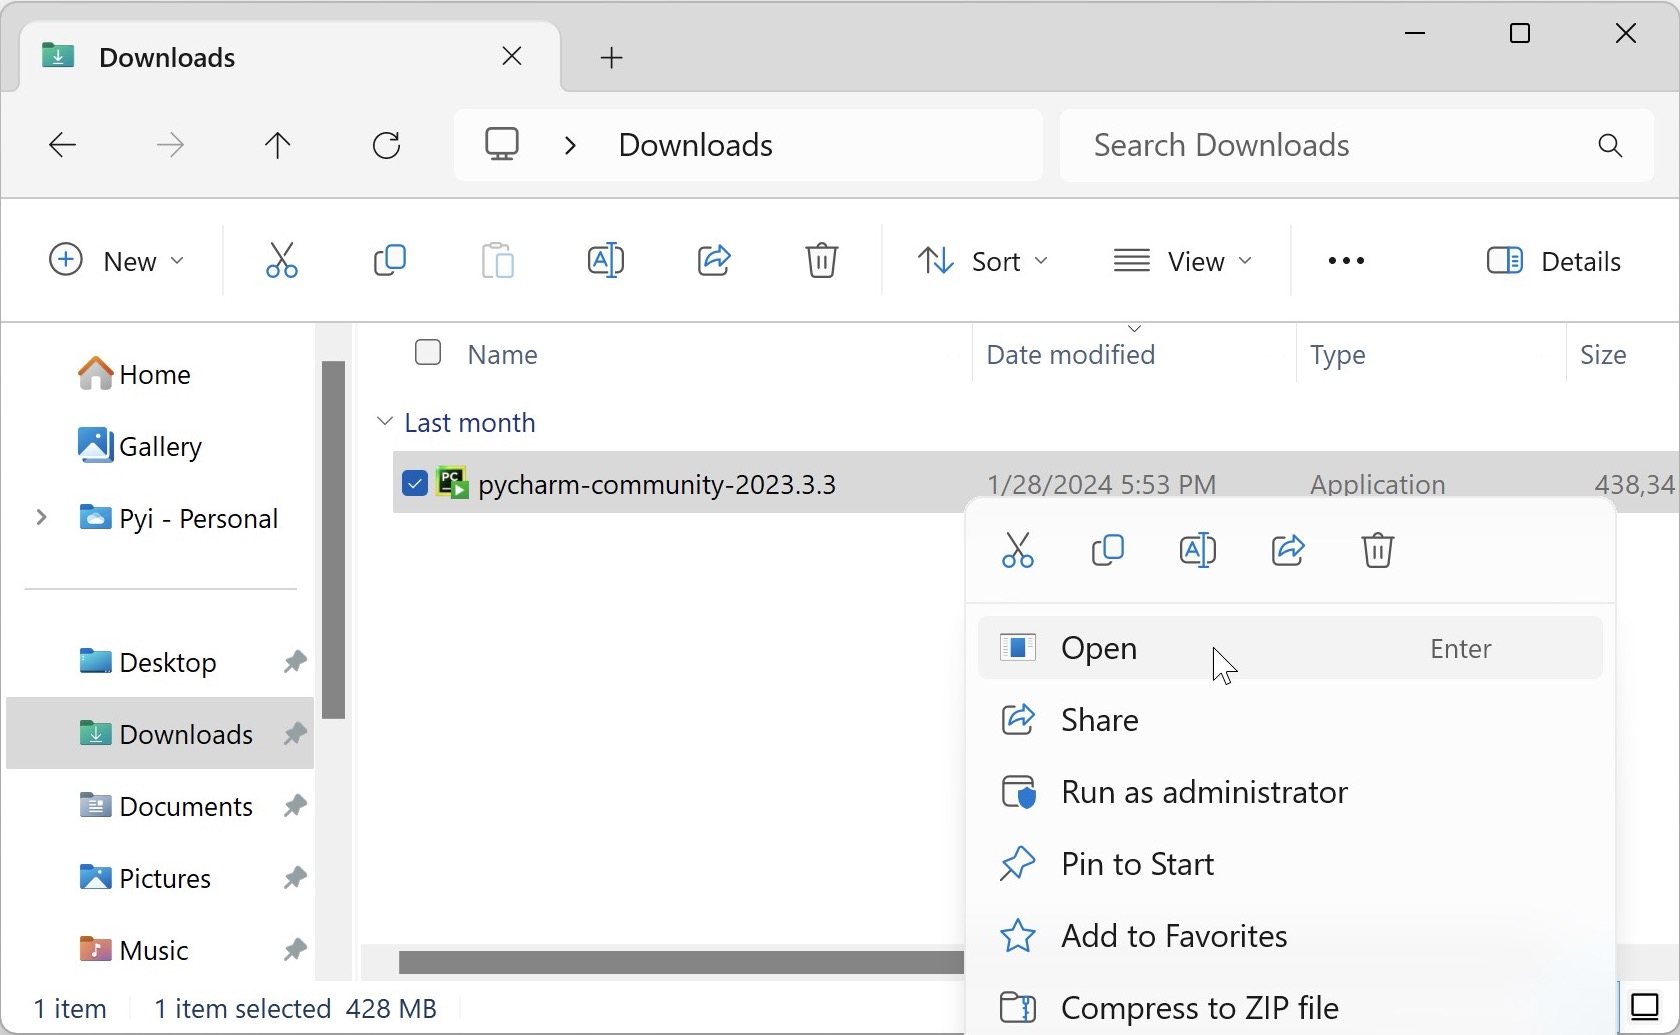
\includegraphics[width=.88\textwidth, trim={2.4mm 12cm 2mm 2mm},clip]{images/pycharm_install/2.jpg}};
    \drawshadow{image}
\end{tikzpicture}
\caption{} 
\label{fig:opnpychminstlr}
\end{figure}

\fEn{\mytcboxinl{PyCharm Community Edition}} ကို ဒေါင်းလုဒ်လုပ်ပါ။ (ဝဘ်စာမျက်နှာ အပေါ်ပိုင်းက ဝယ်သုံးရတဲ့ \fEn{\mytcboxinl{PyCharm Professional}} ကို ဒေါင်းလုဒ် မှားမလုပ်မိဖို့ သတိပြုပါ)။ အင်စတော်လာဖိုင်ကို ညာကလစ်နှိပ်ပြီး \fEnSnd{Open} လုပ်ပါ (ပုံ \fRefNo{\ref{fig:opnpychminstlr}} ကိုကြည့်ပါ)။ \fEnSnd{Yes/No} မေးတဲ့အခါ \fEnSnd{Yes} နှိပ်ပါ။ \mytcboxinl{\fEnSnd{Next >}} ကို နှိပ်၍ ရှေ့ကိုဆက်သွားပြီး နောက်ဆုံးမှာ \mytcboxinl{\fEnSnd{Install}} နှိပ်ပြီး ကွန်ဖန်းလုပ်ပါ။ အင်စတောလ်ပြီးသွားရင် \mytcboxinl{\fEnSnd{Finish}} နှိပ်ပါ။

ဝင်းဒိုး \fEnSnd{Taskbar Search} ကနေ \fEn{PyCharm} ကိုရှာပြီးဖွင့်ပါ (ပုံ \fRefNo{\ref{fig:schpychm}} ကို ကြည့်ပါ)။ သဘောတူကြောင်း ကွန်းဖန်းလုပ်ခိုင်းရင် ချက်ခ်ဘောက်စ် ချက်ခ်လုပ်ပြီး \mytcboxinl{\fEnSnd{Continue}} နှိပ်ပါ။  ဒေတာပို့ချင်လား ထပ်မေးပါလိမ့်မယ်။ \mytcboxinl{\fEnSnd{Don't Send}} နှိပ်ပါ။ \fEnSnd{Welcome} စခရင်ကိုပေါ်လာမယ်။ ပုံ (\fRefNo{\ref{fig:pychmwlcm}}) မှာ ကြည့်ပါ။




\todo{youtube facebook လင့်ထည့်ရန်}

\begin{mytcbox}
ဒီစာရေးနေချိန် လက်ရှိ \fEn{PyCharm} ဗားရှင်းက ၂၀၂၃ ပါ။ သိပ်မကြာခင် ၂၀၂၄ ထွက်ပါတော့မယ်။ အကယ်၍ လက်ရှိဗားရှင်းထက် နိမ့်တဲ့ဗားရှင်းတွေကို ဒေါင်းလုဒ် လုပ်ချင်ရင် အောက်ပါ လင့်ကို သွားပါ။ 
%
\begin{minted}[frame=lines, framerule=0pt]{text}
https://www.jetbrains.com/pycharm/download/other.html
\end{minted}
%
ဗားရှင်း ၂၀၂၄/၂၅ ထွက်ပြီးတဲ့ အချိန်မှာ ၂၀၂၃ ဗားရှင်းကို လိုချင်ရင် ဝဘ်စာမျက်နှာမှ ရှာပြီး ဒေါင်းလုဒ် လုပ်ပါ။ ၂၀၂၃ မှာလည်း ဗားရှင်းအခွဲတွေ ရှိပါသေးတယ်။ လက်ရှိအမြင့်ဆုံး ဗားရှင်းအခွဲ (ဥပမာ ၂၀၂၃.၃.၃) ကို သုံးလို့ရပါတယ်။ ၂၀၂၄/၂၅ သုံးမယ်ဆိုရင်လည်း ပြဿနာတော့ မရှိပါဘူး။ \fEn{Update} ဗားရှင်းဖြစ်တဲ့အတွက် ပုံတွေမှာ ပြထားတာနဲ့တော့ ကွာခြားချက်တချို့ ရှိကောင်းရှိနိုင်ပါတယ်။
\end{mytcbox}
%

\begin{figure}[tbh!]
\begin{tikzpicture}
    \node[anchor=south west,inner sep=0] (image) at (0,0)
        {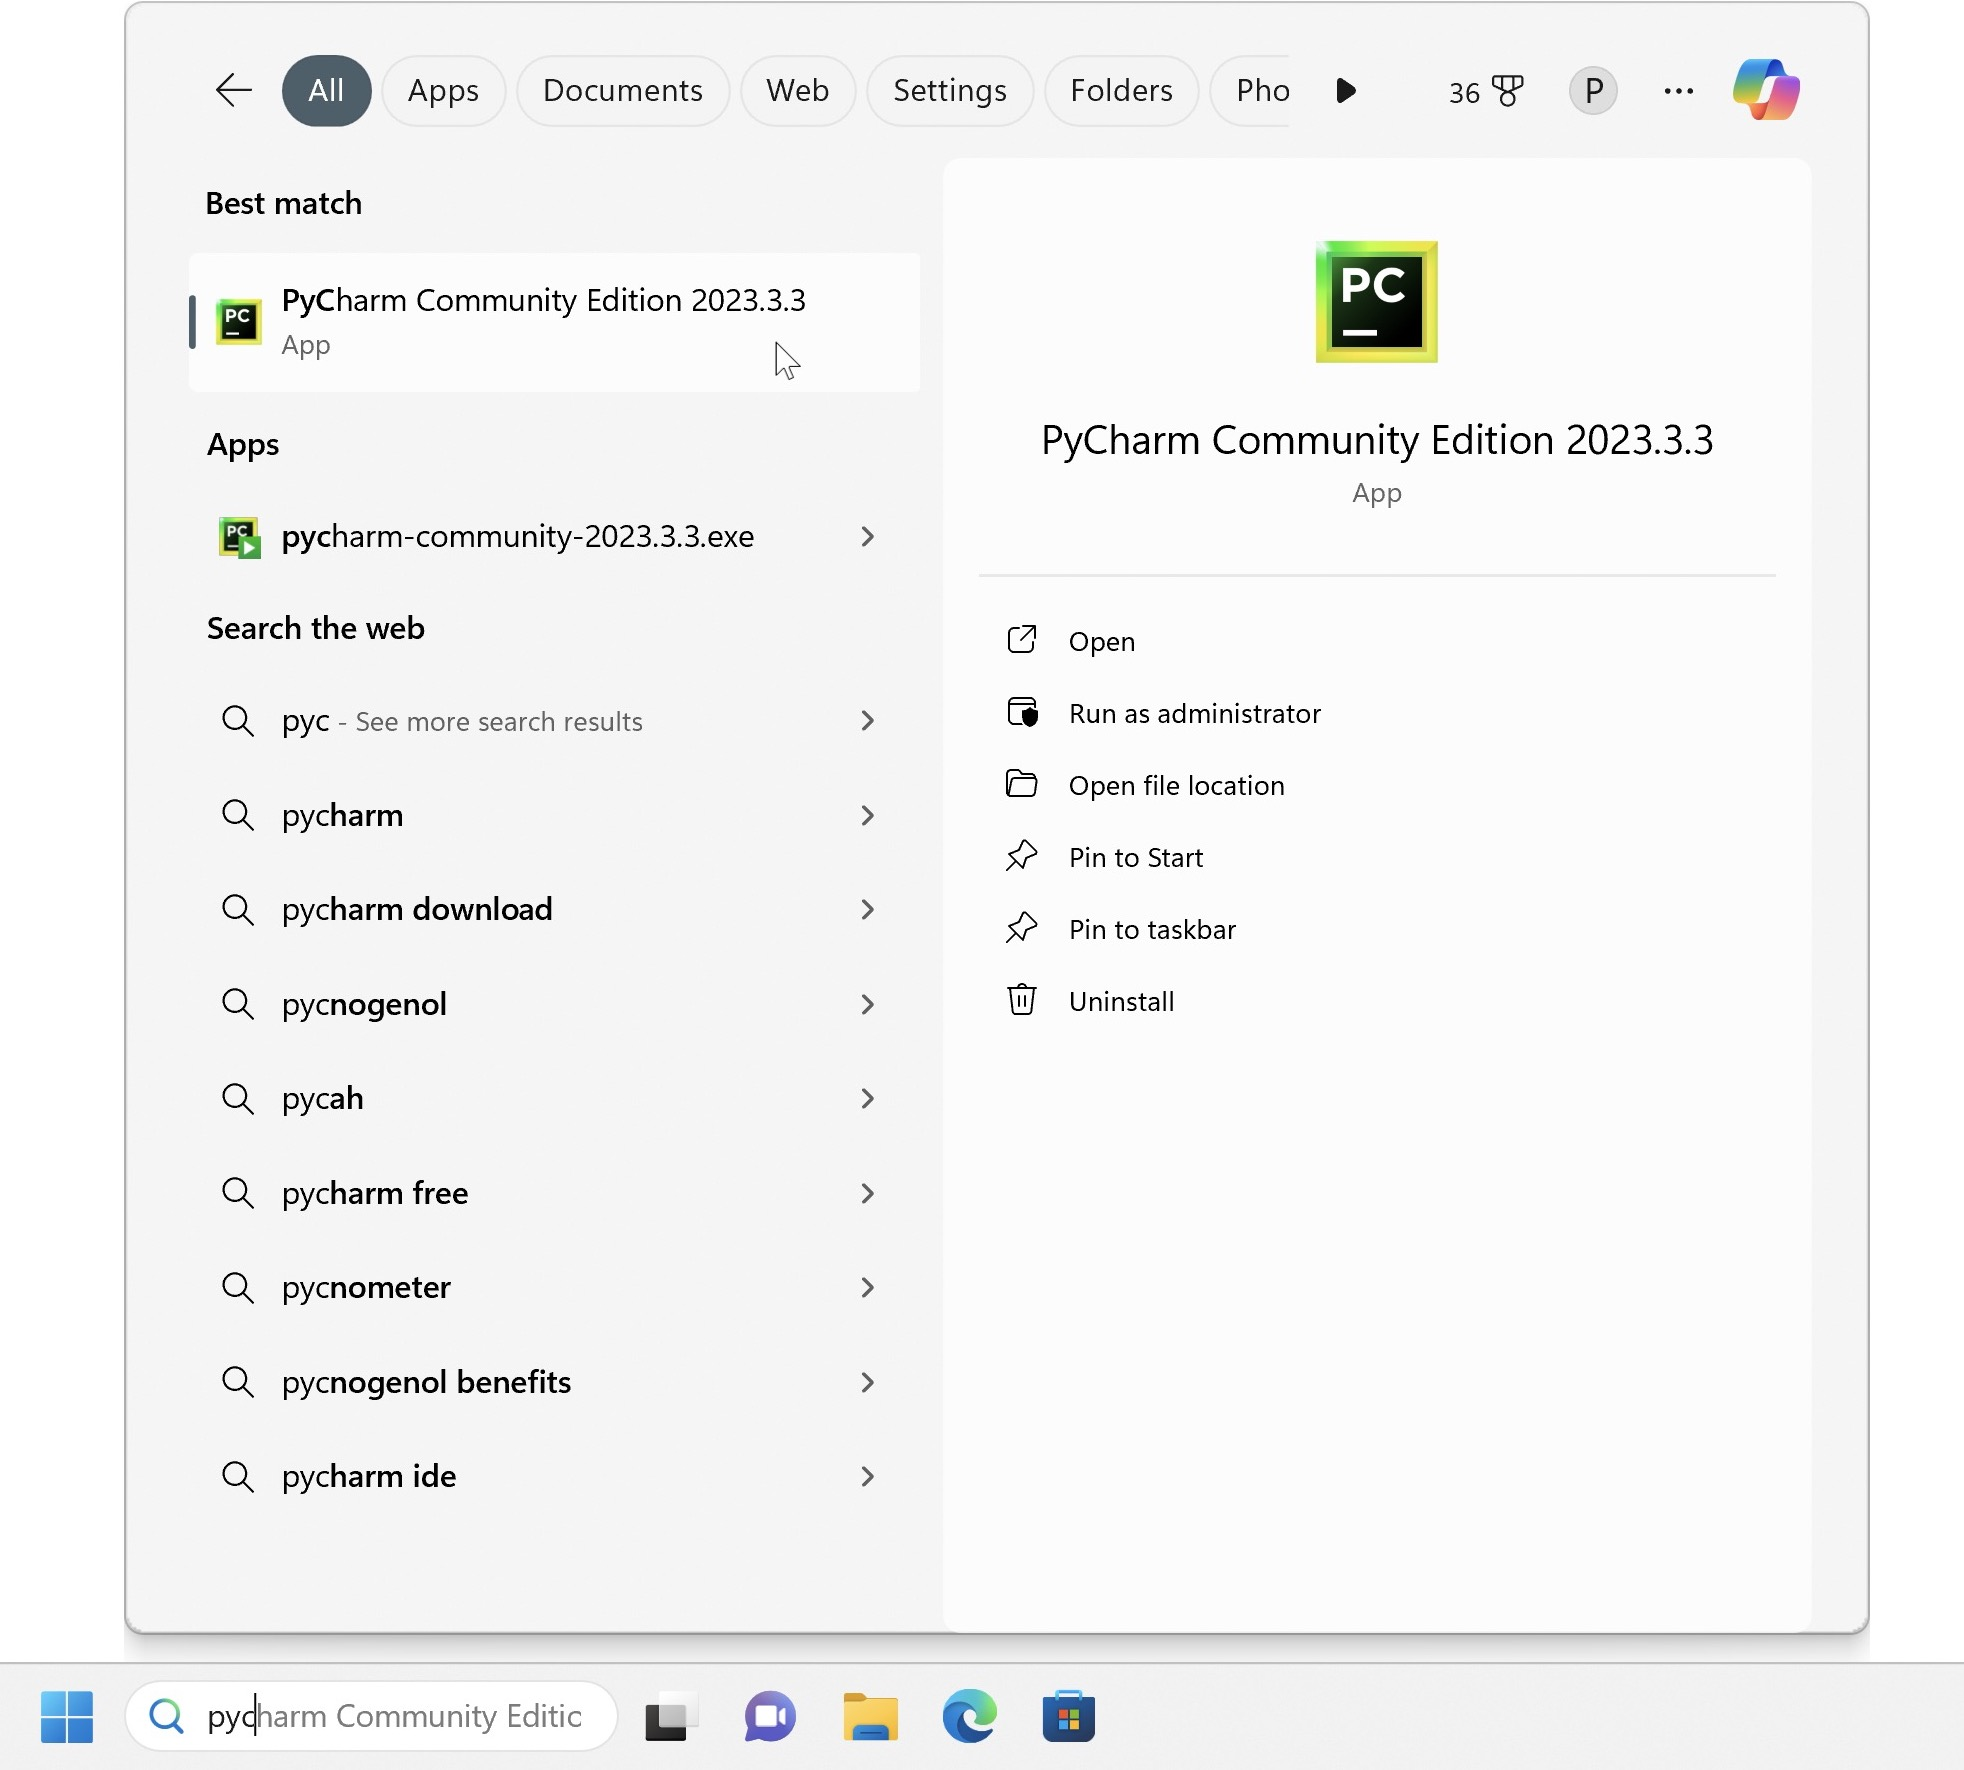
\includegraphics[width=.9\textwidth, trim={2.4mm 2mm 2mm 2mm},clip]{images/pycharm_install/3.jpg}};
    \drawshadow{image}
\end{tikzpicture}
\caption{} 
\label{fig:schpychm}
\end{figure}

\begin{figure}[H]
\begin{tikzpicture}
    \node[anchor=south west,inner sep=0] (image) at (0,0)
        {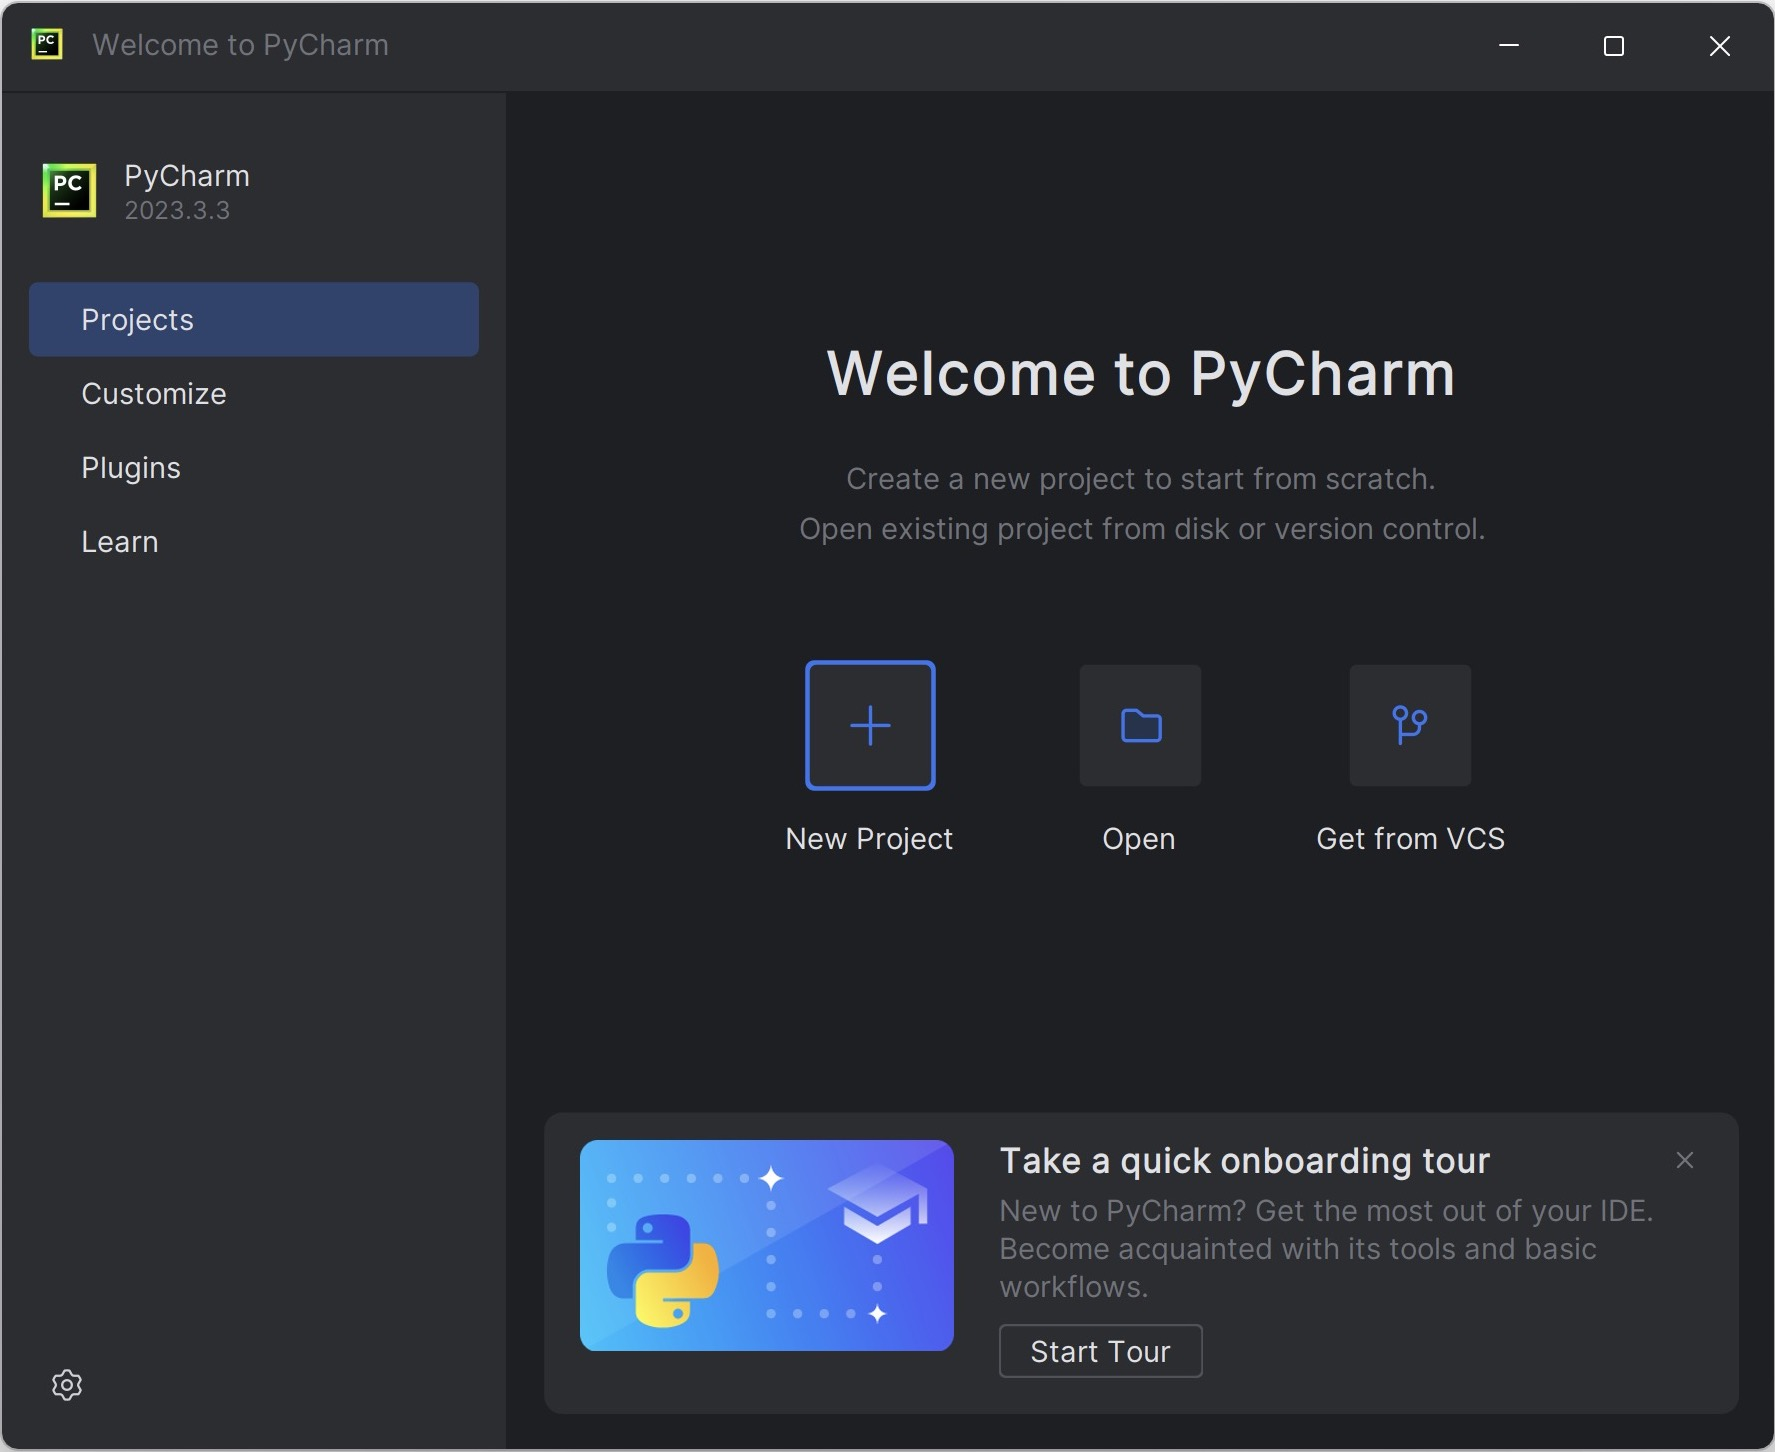
\includegraphics[width=.98\textwidth, trim={2.4mm 2mm 2mm 2mm},clip]{images/pycharm_install/4.jpg}};
    \drawshadow{image}
\end{tikzpicture}
\caption{} 
\label{fig:pychmwlcm}
\end{figure}

\subsection*{PyCharm IDE ဆိုတာဘာလဲ}
\fEn{PyCharm} ဟာ \fEn{Python} နဲ့ ဆော့ဖ်ဝဲ  ရေးဖို့အတွက် အထောက်အကူပြု \fEn{Integrated Development Environment(IDE)} ဆော့ဖ်ဝဲဖြစ်ပါတယ်။ စာစီစာရိုက်လုပ်တဲ့အခါ \fEn{Microsoft Word} ကို အသုံးပြုကြသလိုပဲ \fEn{Python} ကုဒ်ရေးဖို့ \fEn{PyCharm} ကိုသုံးတဲ့ သဘောပေါ့။ \fEn{PyCharm IDE} က \fEn{Python} ပရောဂျက်တွေ အတွက် အဓိကရည်ရွယ်တယ်။ အဆောက်အဦးတစ်ခု၊ တံတားတစ်ခု ဆောက်လုပ်တာကို ပရောဂျက်လို့ ပြောလေ့ရှိသလို ပရိုဂရမ်/ဆော့ဖ်ဝဲတစ်ခု တည်ဆောက်တာကိုလည်း ပရောဂျက်လို့ပဲ သုံးနှုန်းပါတယ်။ တစ်ဦးတစ်ယောက်တည်း ရေးတဲ့ ပရိုဂရမ်အသေးလေးတွေ အတွက် \fEn{PyCharm} ကို အသုံးပြုနိုင်သလို ပရိုဂရမ်မာတွေ အဖွဲ့လိုက်နဲ့ တည်ဆောက်ရတဲ့ ပရောဂျက်ကြီးတွေ အတွက်လည်း သုံးပါတယ်။ ဒီစာအုပ်မှာတော့ \fEn{PyCharm} ရဲ့ အဆင့်မြင့်ဖီချာတွေကို အသုံးပြုမှာ မဟုတ်ပါဘူး။ ပရိုဂရမ်းမင်း စလေ့လာသူတွေကို လွယ်ကူအဆင်ပြေစေတဲ့ အခြေခံ ဖီချာတွေလောက်ပဲ အသုံးပြုမှာပါ။ 

\clearpage

\subsection*{PyCharm ပရောဂျက်ဆောက်ခြင်း}
အင်စတောလ်လုပ်ပြီးရင် \fEn{PyCharm IDE} ကိုဖွင့်ပြီး \fEnSnd{Welcome} စခရင်မှ သိုမဟုတ် \fEnSnd{File} မီနူးမှ \fEnSnd{New Project} နှိပ်ပြီး ပရောဂျက် အသစ်ယူပါ (ပြီးခဲတဲ့ ပုံ \fRefNo{\ref{fig:pychmwlcm}} ကို ပြန်ကြည့်ပါ)။ နံမည်ကို \fEnSnd{MeetKarel} ပေးပါ။ ပုံ (\fRefNo{\ref{fig:new_proj}}) မှာ တွေ့ရတဲ့အတိုင်း \fEnSnd{\mytcboxinl{Pure Python}, \mytcboxinl{Proj venv}} နဲ့ \fEn{Python} ဗားရှင်း \fEnSnd{3.12.xx} ကို ရွေးပါ။ \fEnSnd{xx} က အခြားဂဏန်း ဖြစ်နေနိုင်တယ်။ အဓိက ဗားရှင်း \fEnSnd{3.12} သာ ဖြစ်ပါစေ။ \fEnSnd{Create} ခလုတ်နှိပ်ပါ။ ပရောဂျက်အတွက် \fEn{Python} ကို အင်စတောလ် လုပ်ပါလိမ့်မယ်။

မိမိလေ့လာနေတဲ့ အခန်းတစ်ခန်းချင်းစီအတွက် ပရောဂျက်တစ်ခု ဆောက်နိုင်ပါတယ်။ အခန်း (၂) အတွက် \fEnSnd{Chapter02} ၊ အခန်း (၃) အတွက် \fEnSnd{Chapter03} စသည်ဖြင့်။  သက်ဆိုင်ရာအခန်းအလိုက် ကုဒ်ဖိုင်တွေကို ပရောဂျက်တစ်ခုစီမှာ ထားတဲ့အတွက် ဖိုင်တွေများပြီး ရှုပ်ထွေဖောင်းပွနေတဲ့ ပြဿနာ မရှိတော့ဘူး။ ကုဒ်ဖိုင်တွေကို ပရောဂျက်တစ်ခုထဲမှာပဲ ဖိုဒါအလိုက်ခွဲထားလို့ရပေမဲ့ စလေ့လာသူအနေနဲ့ ပရောဂျက်တစ်ခုချင်း ခွဲထားတာလောက် မလွယ်ကူဘူး။

ပရောဂျက် အသစ်ယူတဲ့အခါ တည်နေရာ \mytcboxinl{\fEnSnd{Location:}} ကို သူ့နဂိုအတိုင်း ထားနိုင်သလို မိမိထားချင်တဲ့နေရာကို ညာဘက်စွန်း ဖိုဒါအိုင်ကွန်လေးနှိပ်ပြီး ပြောင်းလို့ရတယ်။

\begin{figure}[tb!]
\begin{tikzpicture}
    \node[anchor=south west,inner sep=0] (image) at (0,0)
        {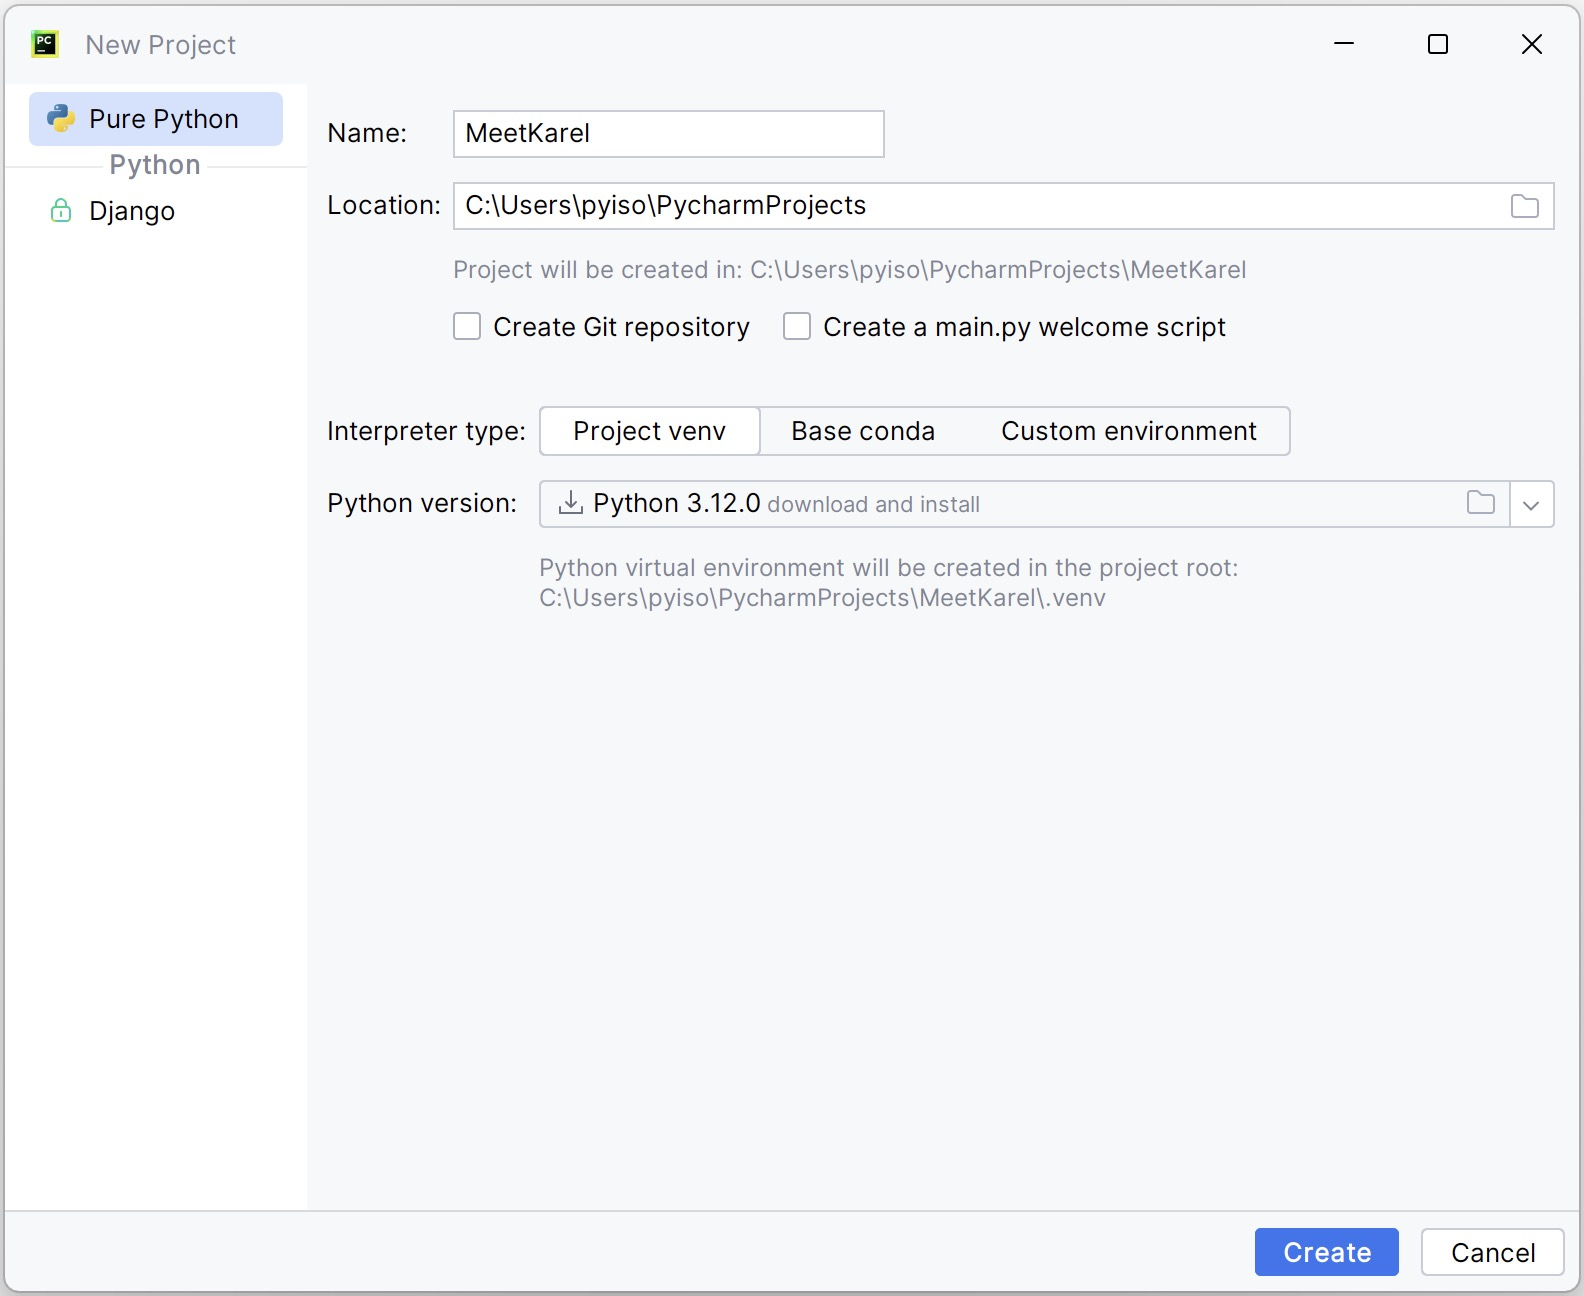
\includegraphics[width=.98\textwidth, trim={2.3mm 2mm 2mm 2.3mm},clip]{images/pycharm_install/new_proj.jpg}};
    \drawshadow{image}
    \draw [draw=red,very thick,rounded corners] (0.15,9.82) rectangle (2.3,9.31);
    \draw [draw=red,very thick,rounded corners] (4.3,7.27) rectangle (6.21,6.76);
    \draw [draw=red,very thick,rounded corners] (4.3,6.68) rectangle (8,6.17);

\end{tikzpicture}
\caption{ပရောဂျက် အသစ်ယူခြင်း} 
\label{fig:new_proj}
\end{figure}

\begin{figure}[tb!]
\begin{tikzpicture}
    \node[anchor=south west,inner sep=0] (image) at (0,0)
        {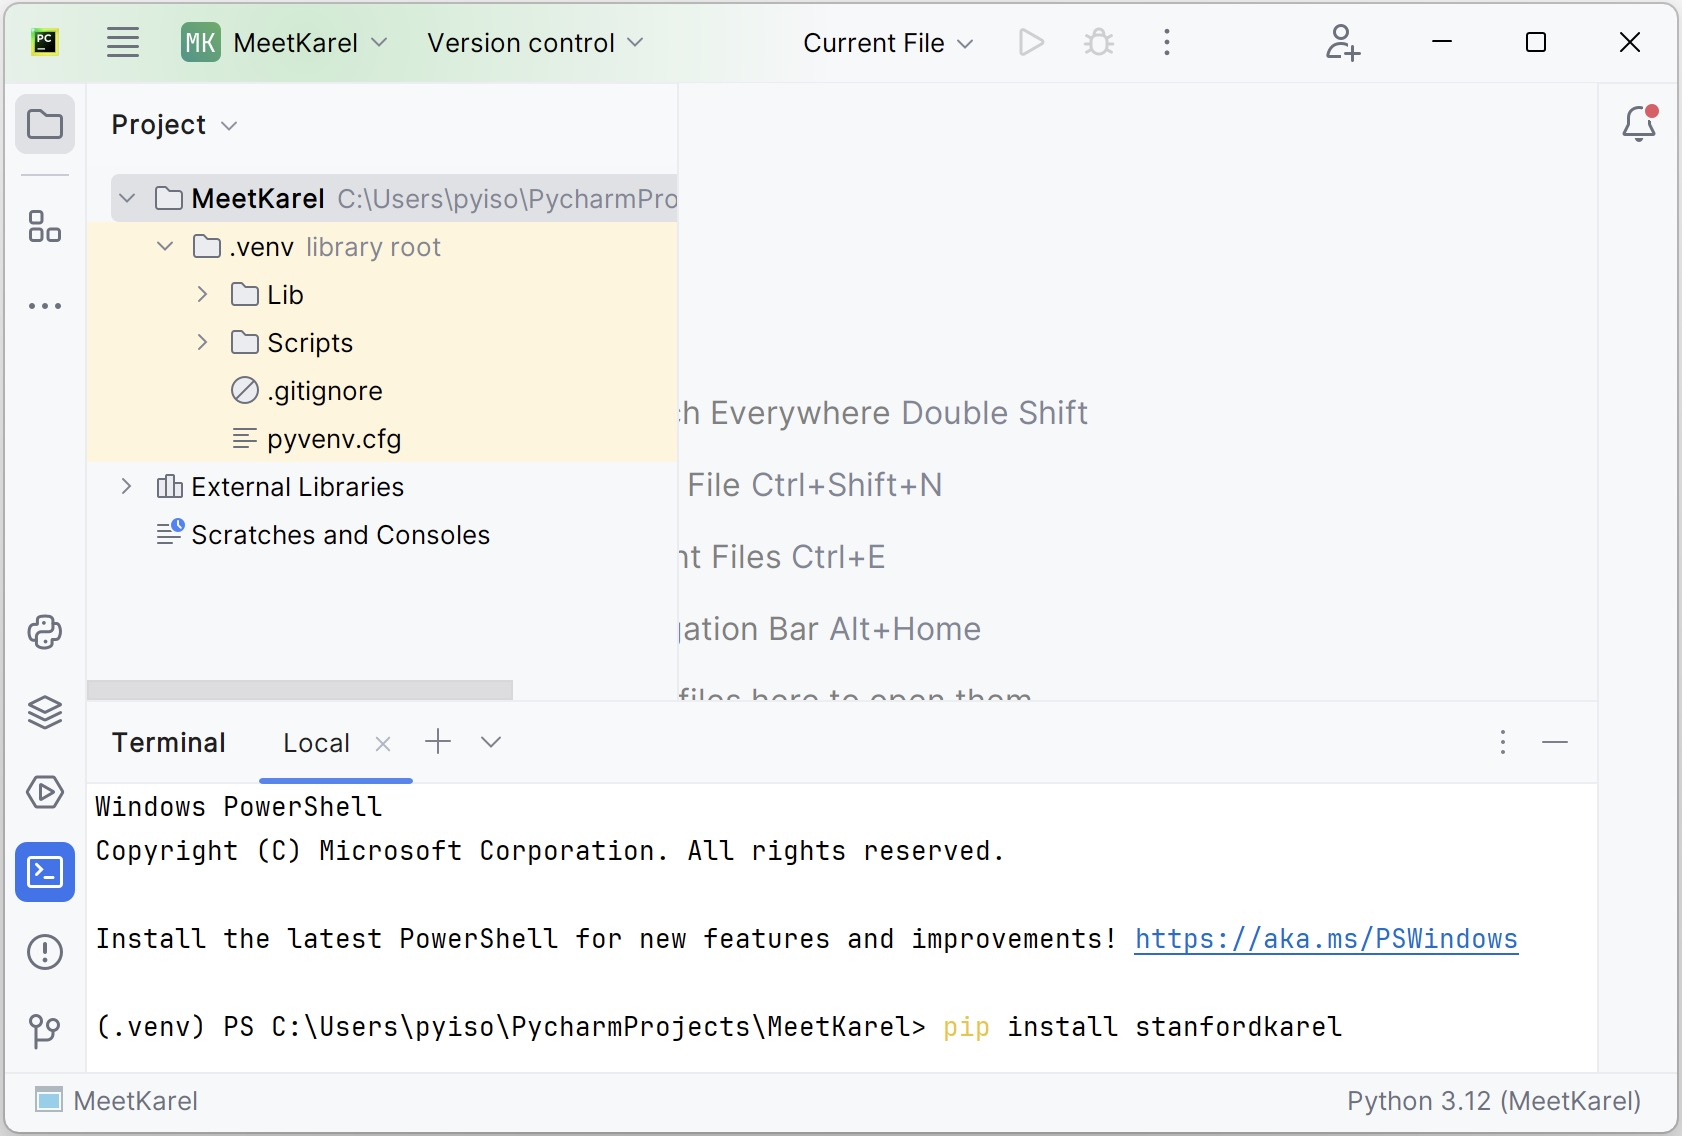
\includegraphics[width=.98\textwidth, trim={2.4mm 2mm 2mm 2.4mm},clip]{images/pycharm_install/install_karel.jpg}};
    \drawshadow{image}
    \draw [draw=red,very thick,rounded corners] (0.02,2.26) rectangle (0.57,1.71);
    \draw [draw=red,very thick,rounded corners] (7.13,1.1) rectangle (10.4,0.55);
\end{tikzpicture}
\caption{Karel လိုက်ဘရီ အင်စတောလ်လုပ်ခြင်း} 
\label{fig:install_karel}
\end{figure}

\subsection*{stanfordkarel လိုက်ဘရီ အင်စတောလ်လုပ်ခြင်း}
ပုံ (\fRefNo{\ref{fig:install_karel}}) မှာ အနီရောင် ဝိုင်းပြထားတဲ့ အိုင်ကွန်ကို နှိပ်ပြီး \fEnSnd{Terminal} ကိုဖွင့်ပါ။ \fEnSnd{Terminal} မှာ အောက်ပါ ကွန်မန်းဖြင့် 
%
\begin{minted}[frame=lines, framerule=0pt]{text}
pip install stanfordkarel
\end{minted}
%
ကားရဲလ်လိုက်ဘရီကို အင်စတောလ်လုပ်ပါ။ ပုံ (\fRefNo{\ref{fig:install_karel}}) မှာ  အနီရောင် ဝိုင်းပြထားပါတယ်။ ခဏကြာတဲ့အခါ အခုလို \fOpn{မက်ဆေ့ချ်}တွေ ကျလာပါလိမ့်မယ်။ 

%
\begin{minted}[frame=lines, framerule=0pt,escapeinside=ßß]{text}
Collecting stanfordkarel
  Downloading stanfordkarel-0.2.7-py3-none-any.whl (51 kB)
     ━━━━━━━━━━━━━━━━━━━━━━━━━━━━━━━━━━━━━━━━ 51.9/51.9 kB 443.1 kB/s 
    eta 0:00:00
Installing collected packages: stanfordkarel
ß\colorbox{yellow}{Successfully installed stanfordkarel-0.2.7}ß

[notice] A new release of pip is available: 23.2.1 -> 24.0
[notice] To update, run: python.exe -m pip install --upgrade pip
(.venv) PS C:\Users\pyiso\PycharmProjects\MeetKarel>
\end{minted}
%
ဟိုက်လိုက်ပြထားတဲ့ \fOpn{မက်ဆေ့ချ်} တွေ့ရရင် အင်စတောလ်လုပ်တာ အောင်မြင်လို့ပါ။

\begin{mytcbox}
မှတ်ချက်။\qquad ။ ပရောဂျက် အသစ်ဆောက်တိုင်း လိုအပ်တဲ့ လိုက်ဘရီကို တစ်ခါထပ်ပြီး အင်စတောလ် လုပ်ရပါမယ်။ ကားရဲလ်အခန်း ပရောဂျက်တစ်ခုစီအတွက် \fEnSnd{stanfordkarel} လိုက်ဘရီကို အထက်ဖော်ပြပါအတိုင်း အင်စတောလ် လုပ်ဖို့လိုတယ်။
\end{mytcbox}

\clearpage
\subsection*{နမူနာ ကားရဲလ် ကမ္ဘာနှင့် ပရိုဂရမ်ကုဒ် ဖိုင်များထည့်ခြင်း}
\fEnSnd{meet\_karel.zip} ဖိုင်ကို \todo{ဒေါင်းလုဒ်လင့်ထည့်ရန်} ဒီလင့် \fCode{http://tinyurl.com/3mmm9c7j} ကနေ ဒေါင်းလုဒ်လုပ်ပါ။ ၎င်း \fEnSnd{zip} ဖိုင်ကို \fEn{extract} လုပ်ပါ။ \fEnSnd{meet\_karel} နံမည်နဲ့ ဖိုဒါတစ်ခု ရလာပါမယ်။ ၎င်းဖိုဒါထဲမှ အောက်ပါ \fEnSnd{worlds} ဖိုဒါနှင့် \fEnSnd{.py} ဖိုင်အားလုံးကို ကော်ပီလုပ်ပါ။ 
%
\begin{itemize}
    \item \fEnSnd{worlds} 
    \begin{itemize}
        \item \fEnSnd{meet\_karel.w}
        \item \fEnSnd{move\_beeper\_to\_other\_side.w}
    \end{itemize}
    \item \fEnSnd{meet\_karel.py}
    \item \fEnSnd{move\_beeper\_to\_other\_side.py}
    \item \fEnSnd{world\_editor.py}
\end{itemize}
%

\fEnSnd{MeetKarel} ပရောဂျက်ထဲတွင် ကူးထည့်ပါ။ ပင်မ ပရောဂျက် \fEnSnd{MeetKarel} (ပုံ \fRefNo{\ref{fig:edit_meet_karel}} မှာ မြှားပြထား) ပေါ်မှာ ညာကလစ်နှိပ်ပြီး \fEnSnd{Paste} လုပ်ရမှာပါ။ ကော်ပီကူးထည့်လိုက်တဲ့ ဖိုင်တွေက ပုံမှာ တွေ့ရတဲ့အတိုင်း  \fEnSnd{MeetKarel} ဖိုဒါအောက်မှာ ရှိသင့်ပါတယ်။

\begin{mytcbox}
အခန်းအလိုက် နမူနာ ကုဒ်ဖိုင်တွေ ထည့်ပေးထားတဲ့ \fEnSnd{.zip} ဖိုင်တွေကိုလည်း အထက်ပါအတိုင်း အလားတူ လုပ်ရပါမယ်။ ပရောဂျက်အသစ်ဆောက်၊ \fEnSnd{.zip} ဖိုင်ကို ဖြည်၊ ရလာတဲ့ ဖိုဒါထဲက ဖိုင်တွေကို ပင်မ ပရောဂျက် ဖိုဒါထဲ ကော်ပီကူးထည့် ရုံပါပဲ။
\end{mytcbox}

\fEnSnd{meet\_karel.py} ဖိုင်ကို ကလစ်နှစ်ချက်နှိပ် ဖွင့်ပါ။ ပုံ (\fRefNo{\ref{fig:edit_meet_karel}}) မှာ အနီဝိုင်းထားတဲ့  ကုဒ်အယ်ဒီတာ \fEn{(code editor)} ပွင့်လာပါမယ်။ အဲဒီ မူရင်းဖိုင်မှာ အောက်ပါအတိုင်း ဆက်လက် ပြင်ဆင်ဖြည့်စွက်ပါ။
%
\setlength{\fboxsep}{0pt}
\label{lst:mtkrl}
\begin{minted}[frame=\mintframe, framerule=\mintrule,framesep= \mintsep, xleftmargin=\xlftmargin
                , bgcolor=mintbgcolor,rulecolor=mintrulecolor
                , python3=true]{python}
from stanfordkarel import *


def main():
    """Karel code goes here!"""
    move()
    move()
    move()
    pick_beeper()
    turn_left()
    move()
    move()

    turn_left()
    turn_left()
    turn_left()

    move()
    put_beeper()


if __name__ == "__main__":
    run_karel_program("meet_karel")
\end{minted}
%

%http://tinyurl.com/3mmm9c7j
%https://bit.ly/42MhViS

% google drive root folder
%http://tinyurl.com/mkamnasm
%https://bit.ly/3T3tgrA

\begin{mytcbox}
\fEn{run} ထားတဲ့ ပရိုဂရမ်တစ်ခုကို တစ်ခါထပ် \fEn{run} ရင် \mytcboxinl{\fEnSnd{Cancel}} (သို့) \mytcboxinl{\fEnSnd{Stop and Rerun}} လုပ်မှာလားမေးတယ်။ \mytcboxinl{\fEnSnd{Stop and Rerun}} လုပ်ရပါတယ်။
\end{mytcbox}

\fEnSnd{meet\_karel.py} ဖိုင်ကို ညာကလစ်နှိမ်ပြီး \fEnSnd{\mytcboxinl{Run 'meet\_karel'}} လုပ်ပါ (အယ်ဒီတာ ဧရိယာမှာ ညာကလစ်နှိမ်ပြီး \fEnSnd{\mytcboxinl{Run 'meet\_karel'}} လုပ်လို့လည်း ရပါတယ်) ။ ပုံ (\fRefNo{\ref{fig:mtkrlpgm}}) က ကားရဲလ် ပရိုဂရမ် တက်လာရင် \fEnSnd{\mytcboxinl{Run Program}} ခလုတ်ကိုနှိပ်ပါ။ ဘိပါကို ကားရဲလ်က ရွှေ့ပေးပါလိမ့်မယ်။

\begin{figure}[b!]
\begin{tikzpicture}
    \node[anchor=south west,inner sep=0] (image) at (0,0)
        {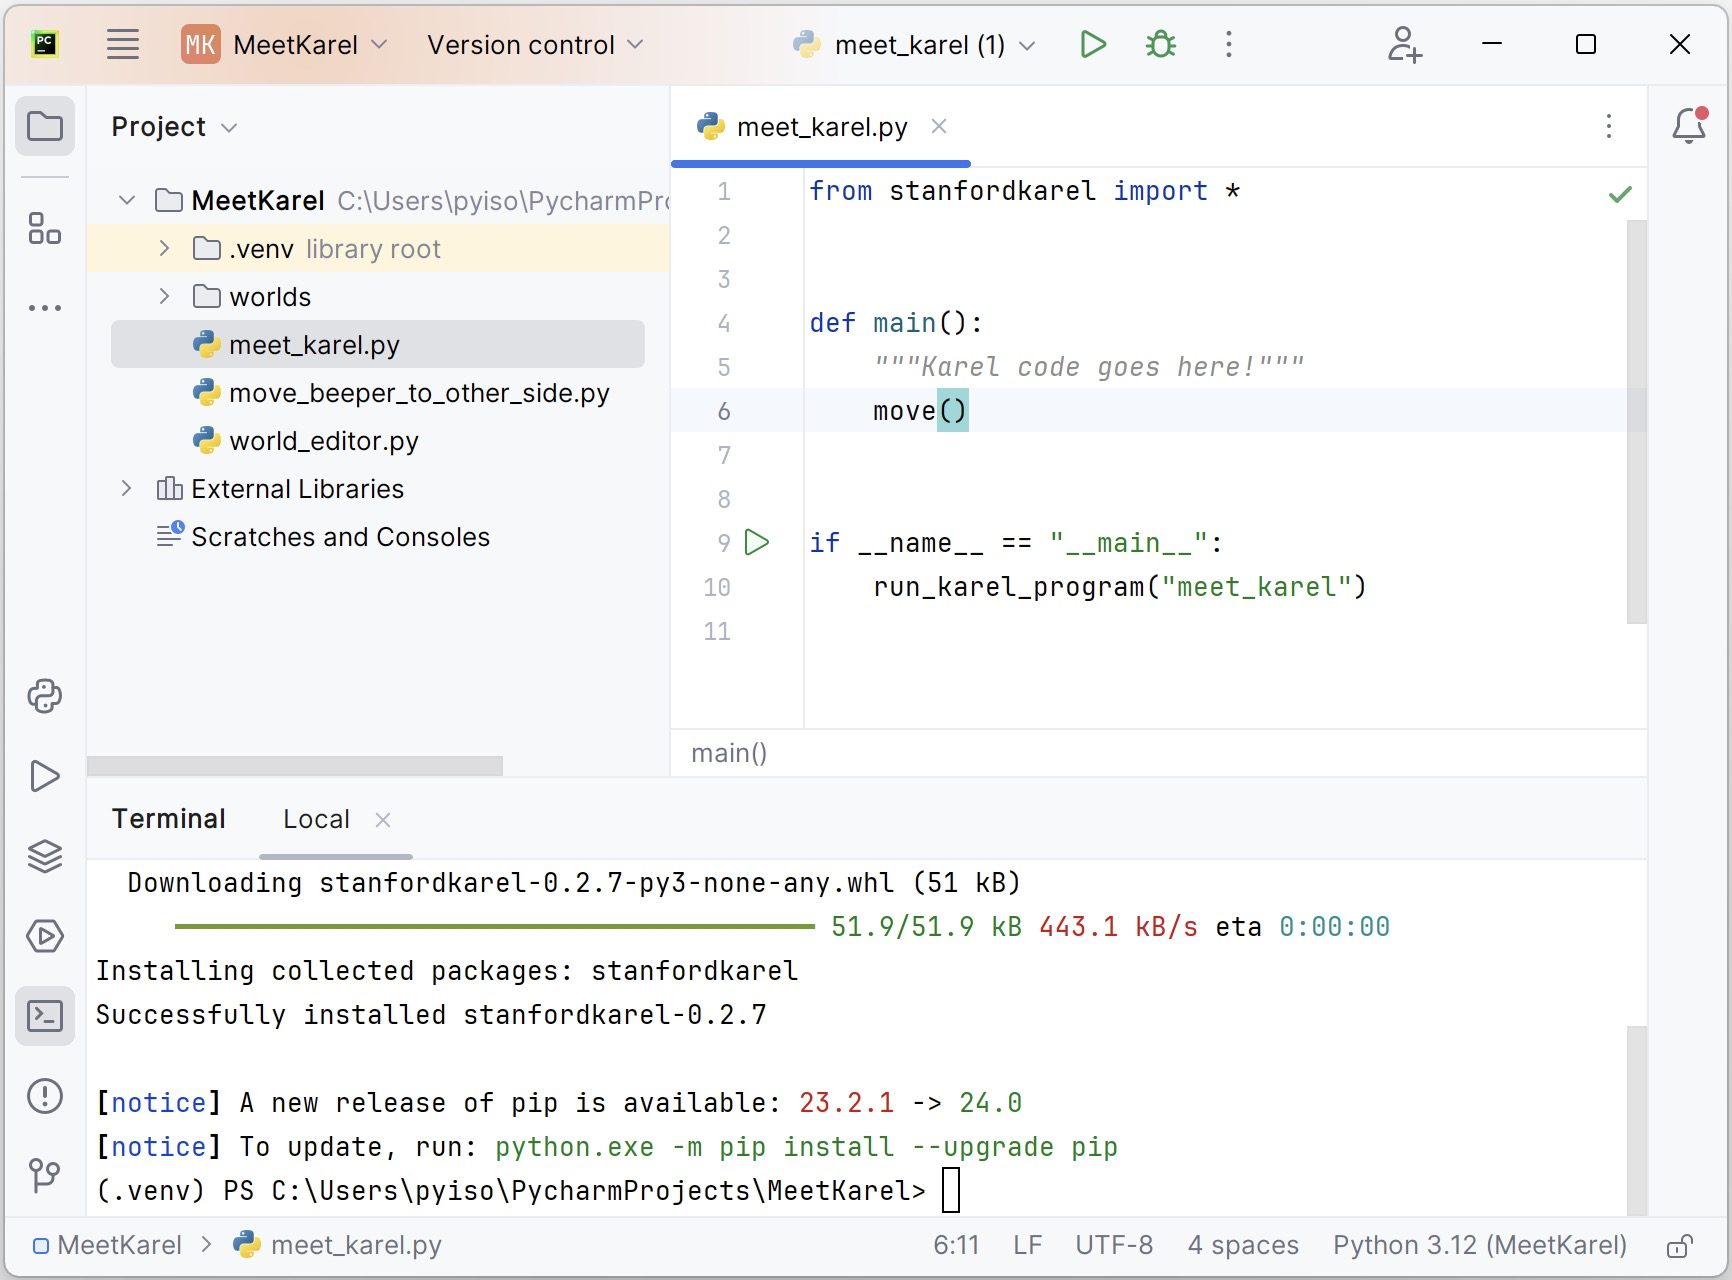
\includegraphics[width=.98\textwidth, trim={2.4mm 2mm 2mm 2.4mm},clip]{images/pycharm_install/edit_meet_karel.jpg}};
    \drawshadow{image}
    
    \draw[-{Latex[length=3mm]}, very thick, red](3, 9)-- (2 ,8.15);
    \draw [draw=red, thick,rounded corners] (5, 8.87) rectangle (12.25 ,3.75);
\end{tikzpicture}
\caption{} 
\label{fig:edit_meet_karel}
\end{figure}


\begin{figure}[b!]
\begin{tikzpicture}
    \node[anchor=south west,inner sep=0] (image) at (0,0)
        {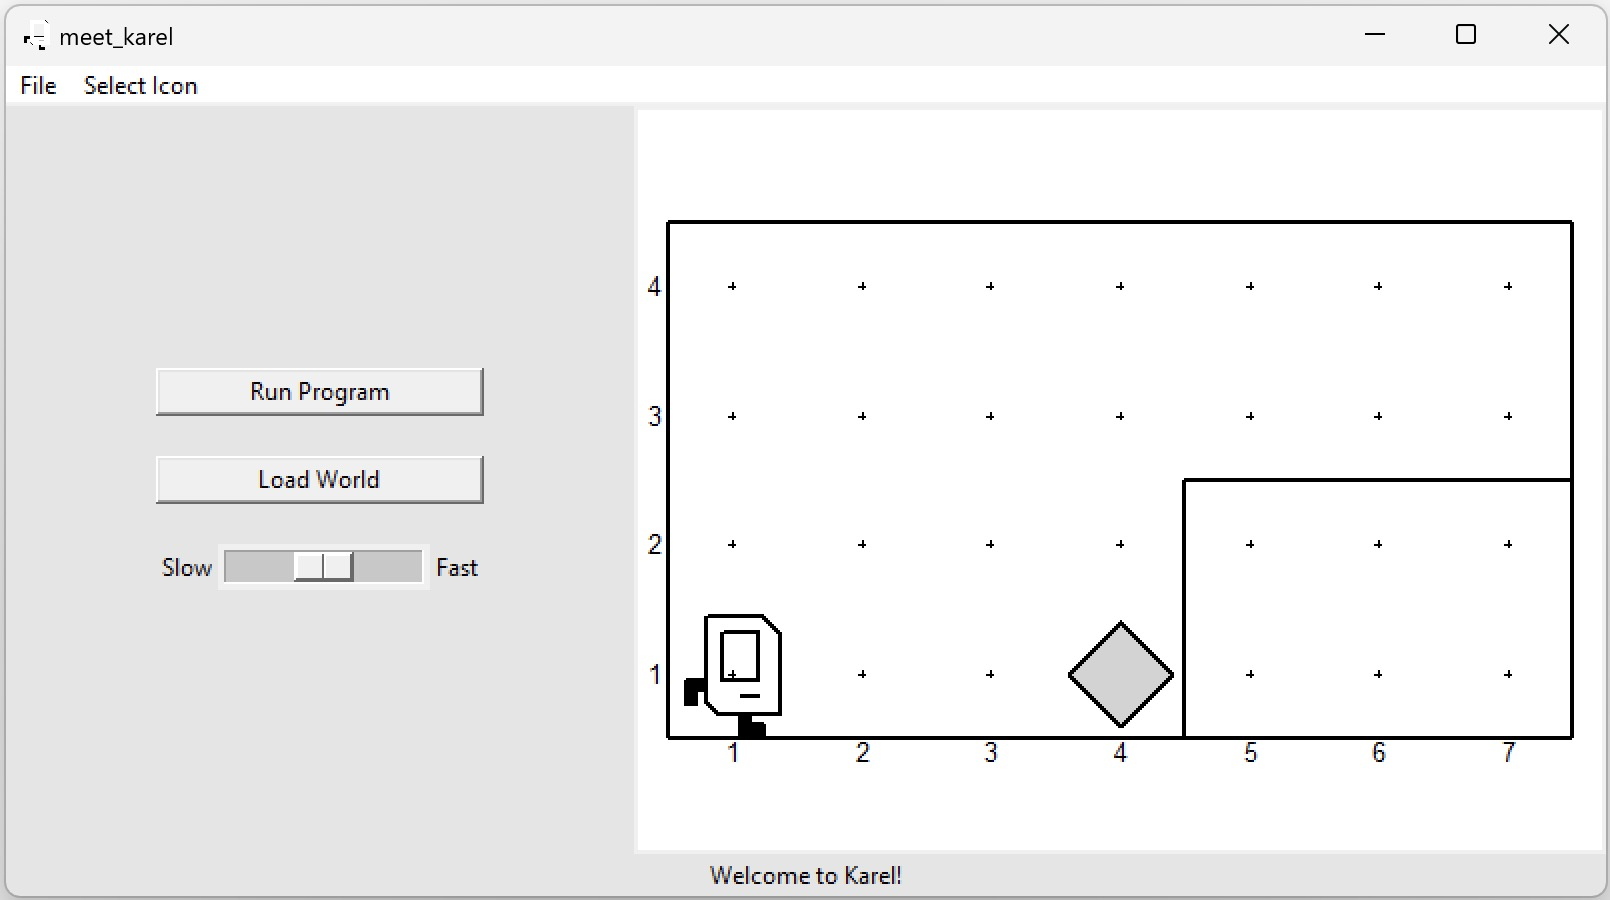
\includegraphics[width=.82\textwidth, trim={2.4mm 2cm 2mm 2mm},clip]{images/pycharm_install/meet_karel_program.jpg}};
    \drawshadow{image}
\end{tikzpicture}
\caption{} 
\label{fig:mtkrlpgm}
\end{figure}



\clearpage
\subsection*{ဆင်းတက်စ်အမှားများ}
\begin{figure}[b!]
\begin{tikzpicture}
    \node[anchor=south west,inner sep=0] (image) at (0,0)
        {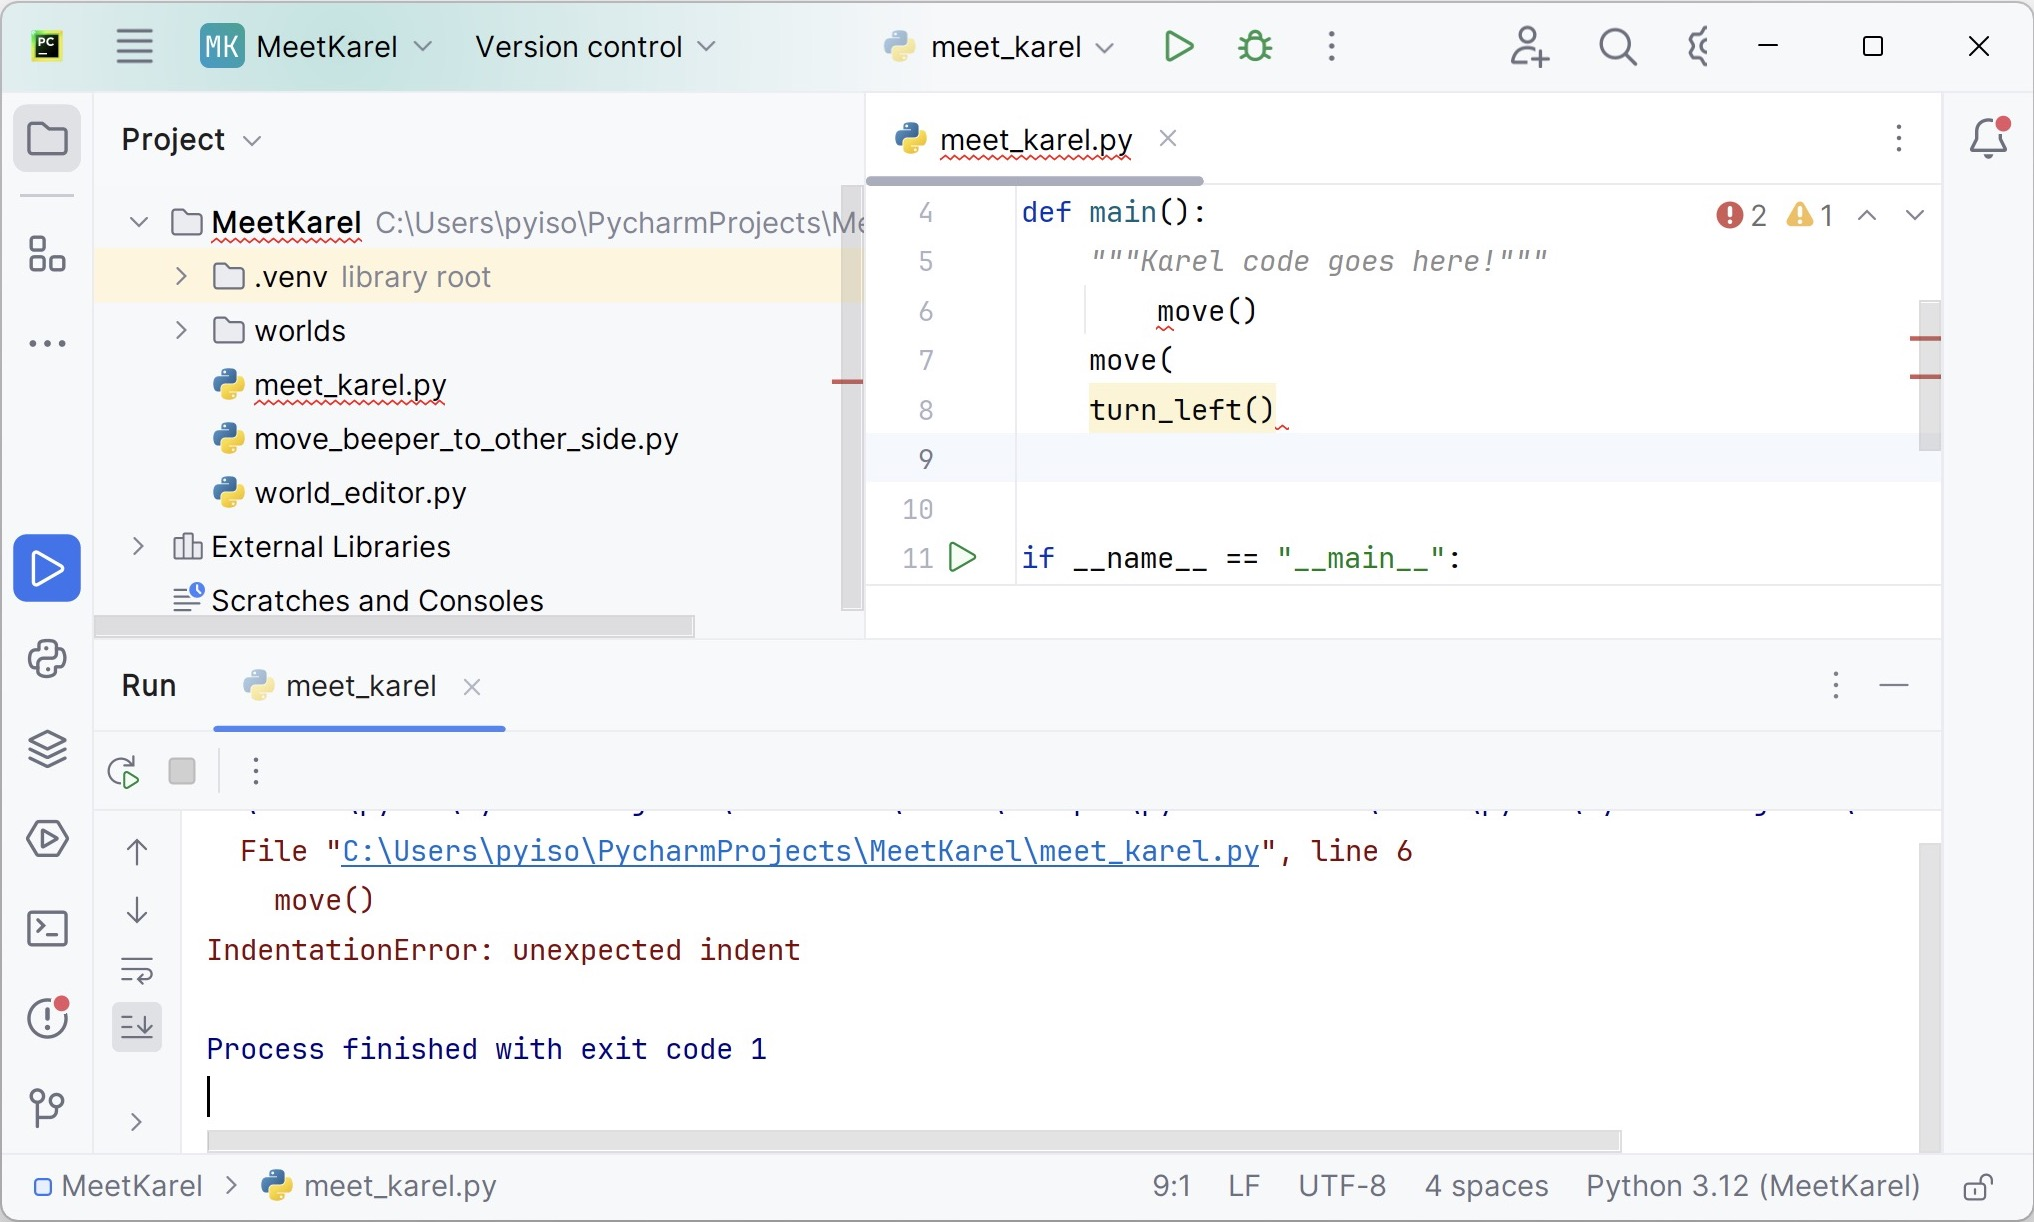
\includegraphics[width=.98\textwidth, trim={2.4mm 2mm 2mm 2mm},clip]{images/pycharm_install/sntxerr.jpg}};
    \drawshadow{image}
\end{tikzpicture}
\caption{} 
\label{fig:sntxerr}
\end{figure}
အကယ်၍ ပရိုဂရမ် \fEn{run} လို့မရရင် ကုဒ်ရေးတာမှားနေလို့ ဖြစ်နိုင်တယ်။ မိမိရေးထားတာကို စာမျက်နှာ (\fRefNo{\pageref{lst:mtkrl}}) က ပရိုဂရမ်ကုဒ်နဲ့  နှိုင်းယှဉ် စစ်ဆေးကြည့်ပါ။ \fEn{PyCharm} အယ်ဒီတာမှာ အနီလှိုင့်တွန့်လေးတွေ (ပုံ \fRefNo{\ref{fig:sntxerr}}) ပြတဲ့နေရင် အဲဒီနေရာတွေမှာ ဆင်းတက်စ်မှားနေလို့ (သို့) လိုက်ဘရီမထည့်ရသေးလို့ပဲ။

ဝိုက်ကွင်းကျန်နေတာက အဖြစ်များတဲ့ အမှားပါ။ ကျန်ခဲ့လို မရပါဘူး။ အင်ဒန့်တေးရှင်း \fEn{(indentation)} လုပ်ရမဲ့နေရာမှာ မလုပ်ထားရင်လည်း ပြဿနာဖြစ်တယ်။ \fCode{move}\fEn{,} \fCode{turn\_left} တွေကို ဘေးမျဉ်းညာဘက်ခွာပြီး အင်ဒန့်လုပ်ပေးရမယ်။ အဲဒါတွေ ဂရုမစိုက်မိရင် ဆင်းတက်စ်အမှားဖြစ်ပြီး ပရိုဂရမ် \fEn{run} လို့ မရနိုင်ဘူး။

\fEnSnd{Terminal} မှာ ထုတ်ပေးတဲ့ \fOpn{မက်ဆေ့ချ်}တွေကို ကြည့်ပြီးတော့လည်း ဘာပြဿနာဖြစ်နေလဲ မှန်းဆလို့ရနိုင်တယ်။ ဘာကြောင့်ဖြစ်နိုင်လဲ ဆက်စပ်စဉ်းစားလို့ ရတယ်။ ဥပမာ ဖြစ်တဲ့ပြဿနာအလိုက် အခုလိုတွေ့ရပါမယ်။ 
%
\begin{minted}[frame=lines, framerule=0pt,escapeinside=ßß]{text}
File "c:\Users\pyiso\VS Code\meet_karel\meet_karel.py", ß\mytcboxinl[yellow]{line 6}ß
    move(
          ^
    ß\mytcboxinl[yellow]{SyntaxError: '(' was never closed}ß
\end{minted}
%
%
\begin{minted}[frame=lines, framerule=0pt,escapeinside=ßß]{text}
File "c:\Users\pyiso\VS Code\meet_karel\meet_karel.py", ß\mytcboxinl[yellow]{line 7}ß
    move()
    ß\mytcboxinl[yellow]{IndentationError: unexpected indent}ß 
\end{minted}
%
%
\begin{minted}[frame=lines, framerule=0pt, escapeinside=ßß]{text}
Traceback (most recent call last):
  File "c:\Users\pyiso\VS Code\meet_karel\meet_karel.py", ß\mytcboxinl[yellow]{line 1}ß, 
        in <module>
    from stanfordkarel import *
    ß\mytcboxinl[yellow]{ModuleNotFoundError: No module named 'stanfordkarel'}ß
\end{minted}
%
\clearpage

\subsection*{Python ဖိုင် အသစ်ယူခြင်း}
\fEnSnd{MeetKarel} ပင်မ ပရောဂျက်ဖိုဒါပေါ်မှာ ညာကလစ်နှိပ်ပြီး \fEn{Python} ဖိုင် အသစ်ယူနိုင်ပါတယ်။ \fEn{Python} ဖိုင်တွေက \fEnSnd{.py} အိပ်စ်တန်းရှင်းနဲ့ပါ။ ကားရဲလ်ပရိုဂရမ်တစ်ခုကို \fEn{Python} ဖိုင်တစ်ခု ထားပါမယ်။ ပင်မ ပရောဂျက်ဖိုဒါ အောက်မှာပဲ တိုက်ရိုက်ရှိရပါမယ်။ 

နောက်ပိုင်း အဆင့်မြင့်လာရင် ပရိုဂရမ်တစ်ခုအတွက် ပရောဂျက်တစ်ခု ထားနိုင်တယ်။ ကုဒ်ဖိုင်တွေအပြင် ပရိုဂရမ်အတွက် လိုအပ်တဲ့ ရုပ်ပုံတွေ၊ အခြားဖိုင်တွေ (\fEn{config} ဖိုင်၊ \fEn{setting} ဖိုင် စသည်ဖြင့်) လည်း ပါနိုင်တယ်။ ပင်မပရောဂျက် အောက်မှာပဲ  ဖိုင်တွေက တိုက်ရိုက်ရှိဖို့လည်း မလိုတော့ဘူး။  ဆက်{\allowbreak}စပ်ရာ ဖိုင်တွေကို အမျိုးအစားအလိုက်၊  ဖန်ရှင်အလိုက် ဖိုဒါတွေခွဲပြီး  စနစ်ကျ စီစဉ်ဖွဲ့စည်း ထားရမှာပါ။ ပရောဂျက်တစ်ခုမှာ ဖိုင်တွေကို စနစ်တကျ စုဖွဲ့ထားဖို့ အရေးကြီးပါတယ်။

\begin{figure}[tbh!]
\begin{tikzpicture}
    \node[anchor=south west,inner sep=0] (image) at (0,0)
        {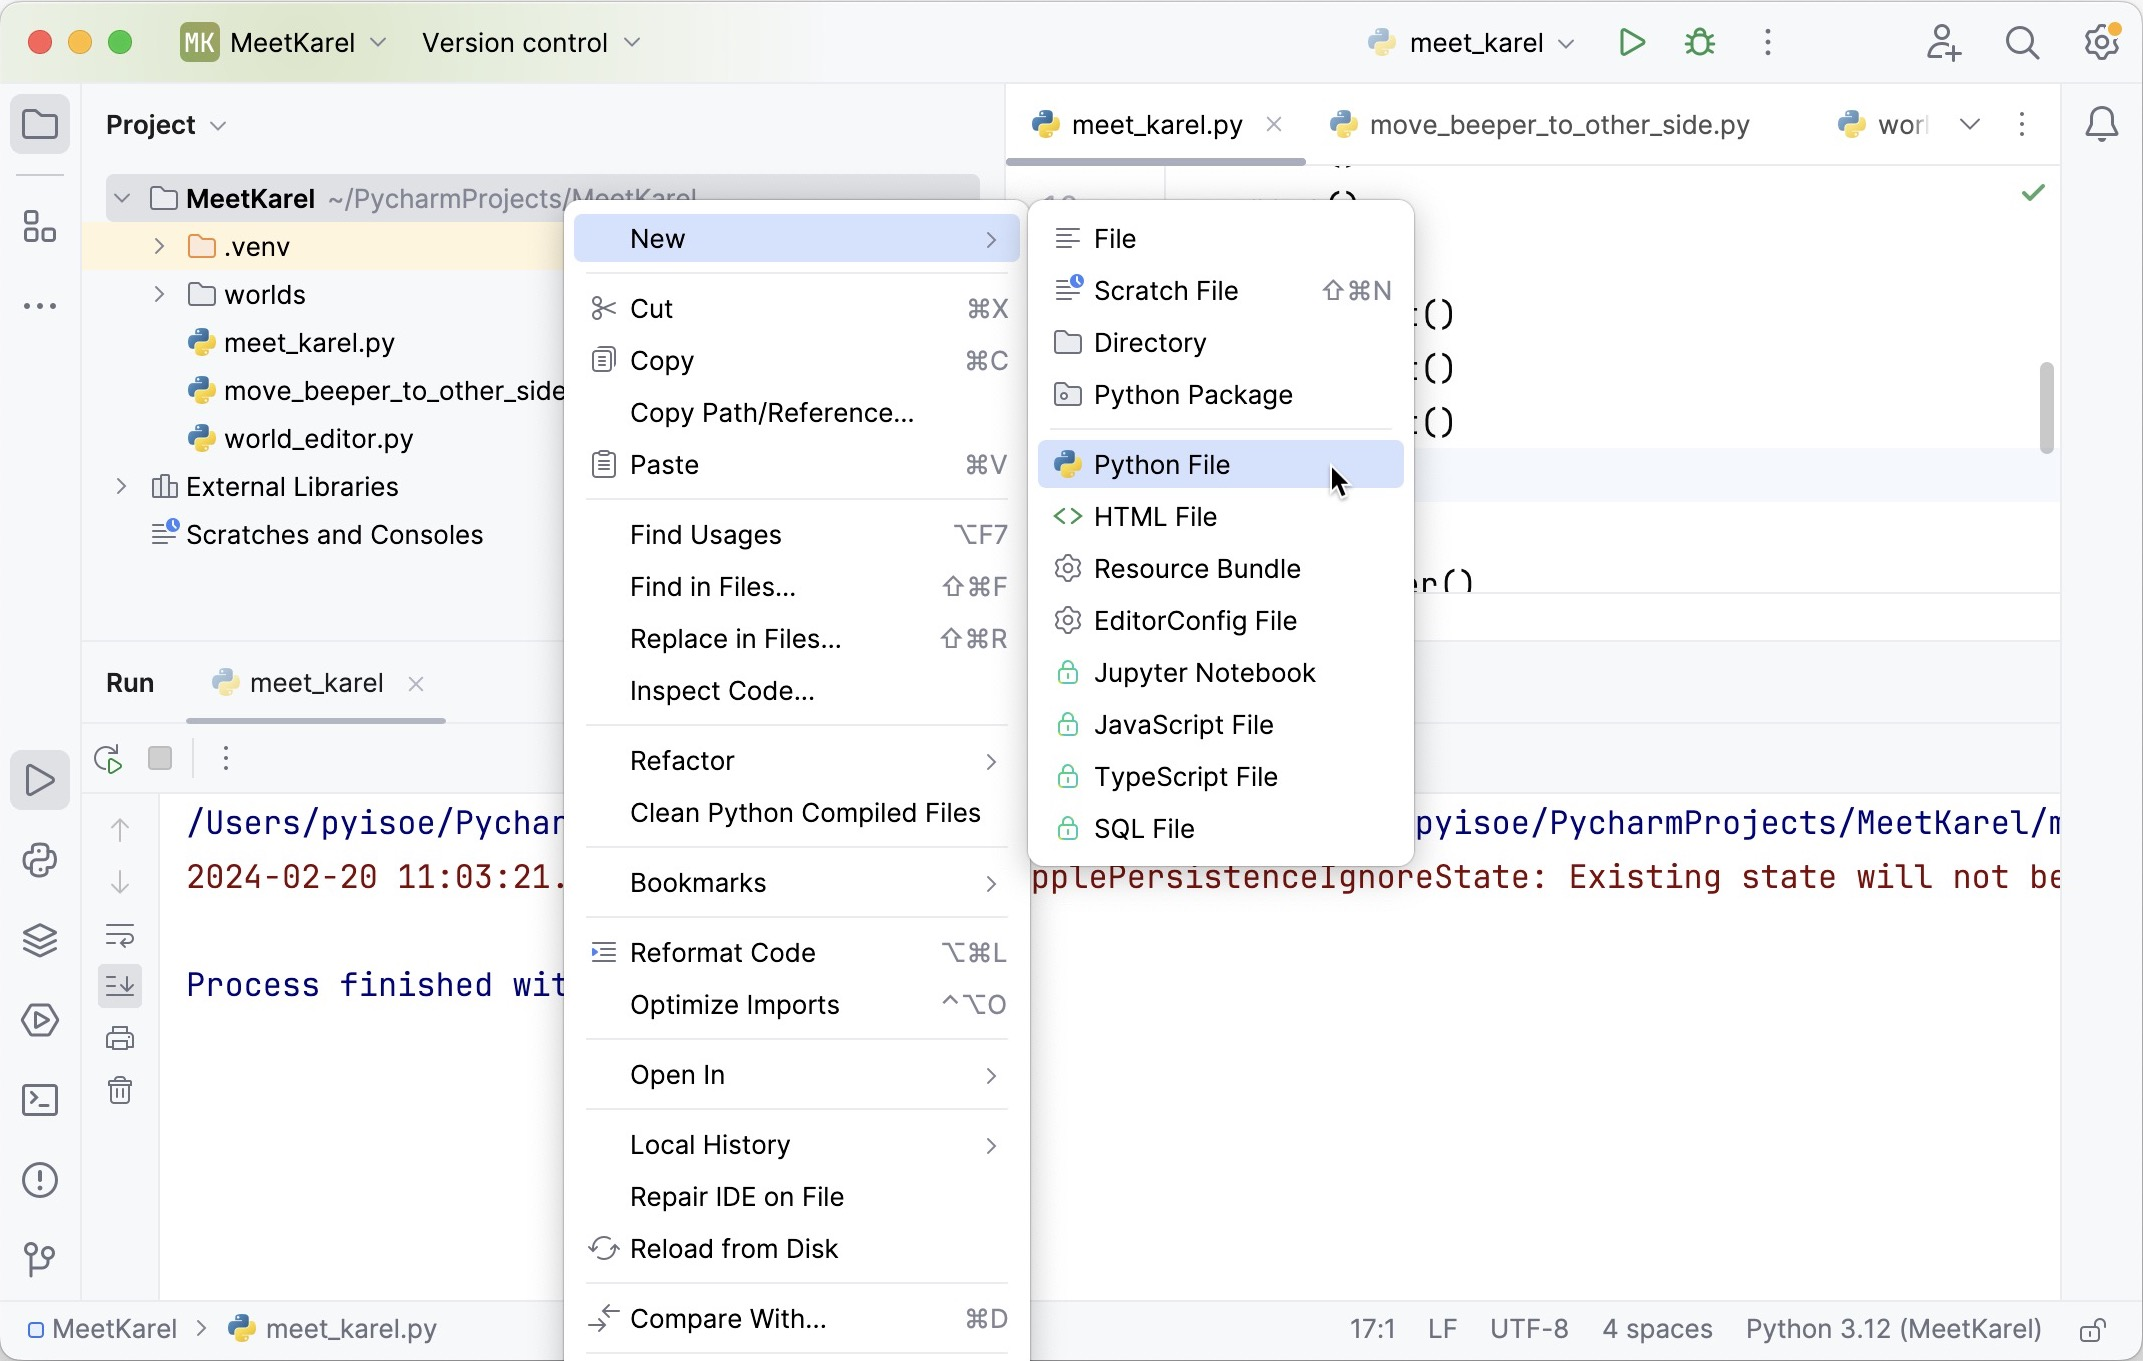
\includegraphics[width=.98\textwidth, trim={2.4mm 2mm 2mm 2mm},clip]{images/pycharm_install/newfile.jpg}};
    \drawshadow{image}
\end{tikzpicture}
\caption{} 
\label{fig:newfile}
\end{figure}

\clearpage



\section*{Visual Studio Code နှင့် Python အင်စတောလ်လုပ်ခြင်း}
\fEn{Visual Studio Code(VS Code)} ဟာ ပရိုဂရမ်မာအများစု ကြိုက်နှစ်သက်တဲ့ မော်ဒန် ကုဒ်အယ်ဒီတာ တစ်ခုပါ။ \fEn{Python, JavaScript, C++} စတဲ့ \fEn{programming language} အမျိုးမျိုးအတွက် အသုံးပြုနိုင်ပါတယ်။

\fEn{PyCharm} မှာတော့ ပရောဂျက်အသစ်ဆောက်ရင် \fEn{Python} ပါ တစ်ခါတည်း ဒေါင်းလုဒ်လုပ်ပြီး အင်စတောလ် လုပ်လို့ရတယ်။  \fEn{VS Code} နဲ့ \fEn{Python} ရေးမယ်ဆိုရင် \fEn{Python Programming Language} ကို သီးခြား ဒေါင်းလုဒ်လုပ်ပြီး အင်စတောလ် လုပ်ရပါမယ်။ 
\subsection*{Python အင်စတောလ်လုပ်ခြင်း}
ဒီလင့် \fCode{https://www.python.org/} ကိုဖွင့်ပါ။ \fEnSnd{Download} မီနူးမှ \fEnSnd{Windows} နှိပ်ပါ (ပုံ \fRefNo{\ref{fig:pyhome}} ကိုကြည့်ပါ)။ \fEn{Apple} ကွန်ပျူတာအတွက် ဆိုရင် \fEnSnd{macOS} ရွေးရပါမယ်။ လူများစုသုံးတဲ့ မိုက်ခရိုဆော့ဖ် ဝင်းဒိုးအတွက် အင်စတောလ်လုပ်နည်းကို အဓိကပြပေးမှာပါ။ ပုံ \fRefNo{\ref{fig:pyvers}} မှာလို တွေ့ရပါလိမ့်မယ်။ အင်စတော်လာ ဗားရှင်း \fEn{3.12} ထဲက လက်ရှိအမြင့်ဆုံး ကိုရွေးပါ။ ဒီစာရေးချိန်မှာ \fEn{3.12.2} ဟာ အမြင့်ဆုံးဗားရှင်းပါ။ \mytcboxinl{\fEnSnd{Windows Installer (64-bit)}} ကိုနှိပ်ပြီး ဒေါင်းလုဒ်လုပ်ပါ။

\todo{linux အတွက် ဖော်ပြရန်}
\begin{figure}[tbh!]
\begin{tikzpicture}
    \node[anchor=south west,inner sep=0] (image) at (0,0)
        {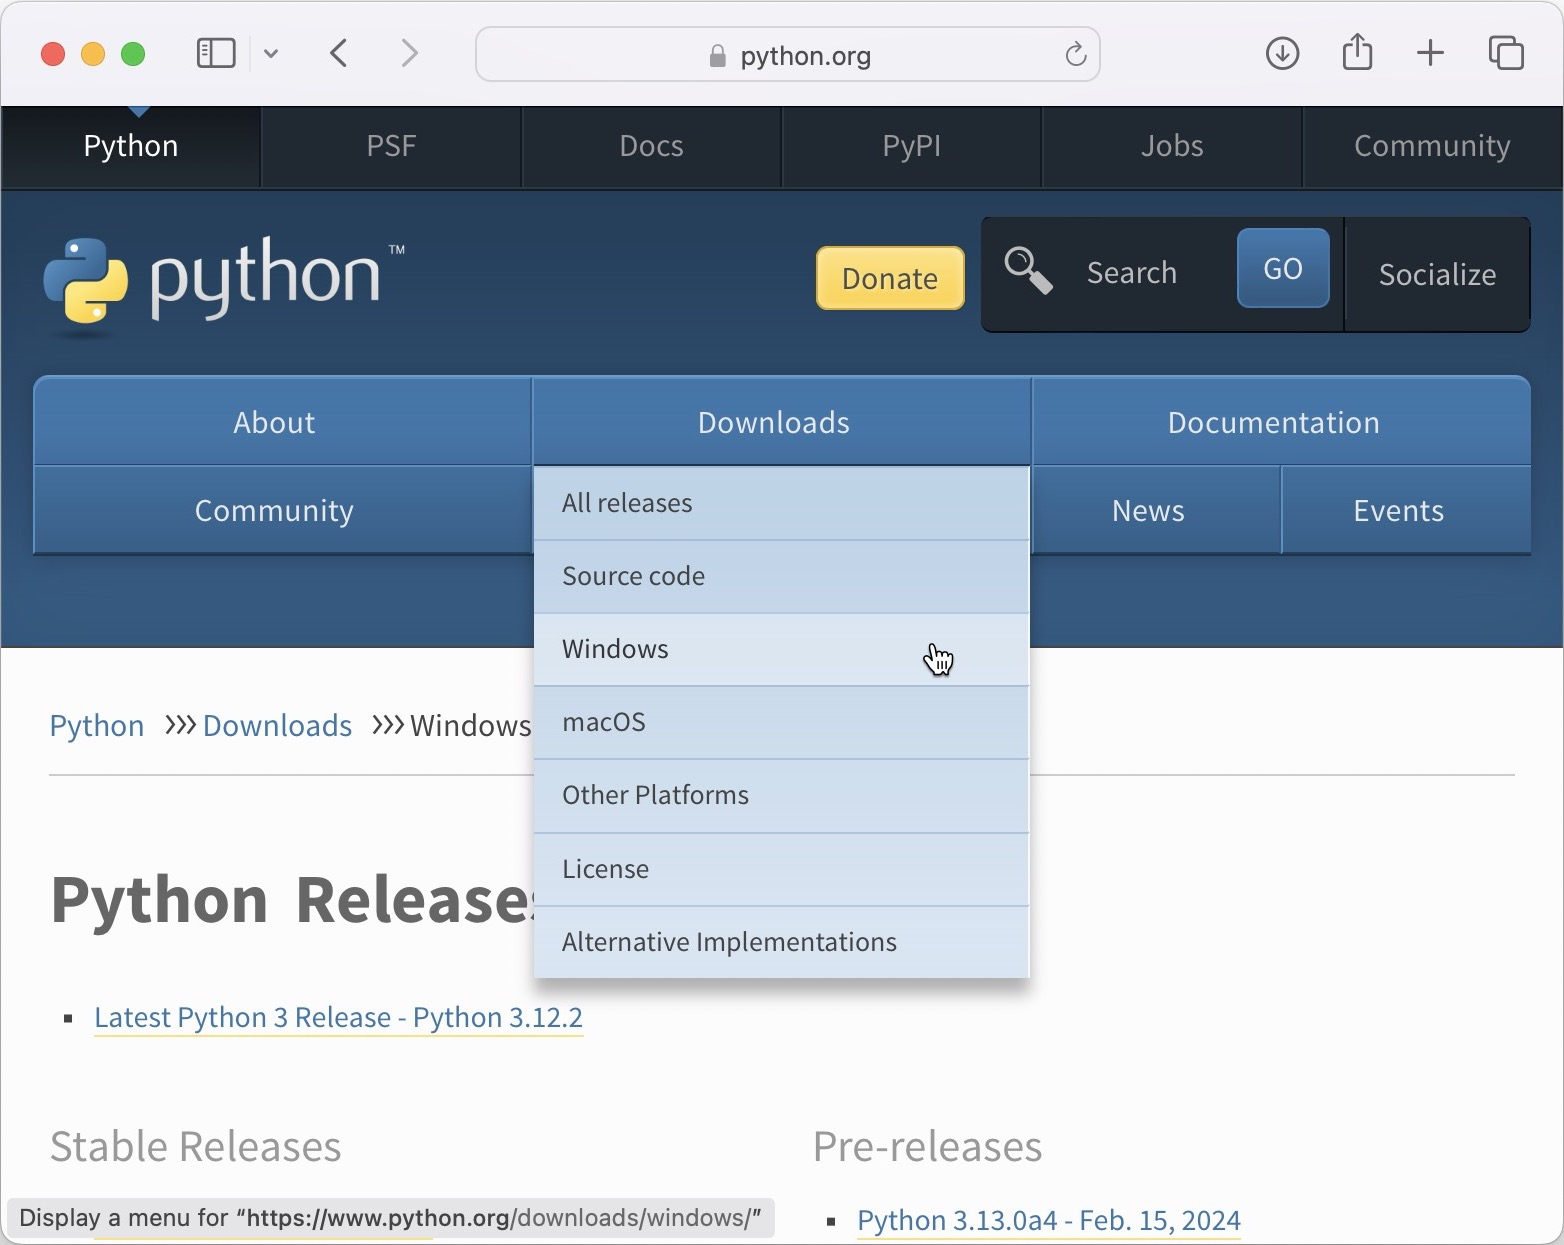
\includegraphics[width=.98\textwidth, trim={2.4mm 2mm 2mm 2mm},clip]{images/vscode_install/1.jpg}};
    \drawshadow{image}
\end{tikzpicture}
\caption{} 
\label{fig:pyhome}
\end{figure}

\begin{figure}[tbh!]
\begin{tikzpicture}
    \node[anchor=south west,inner sep=0] (image) at (0,0)
        {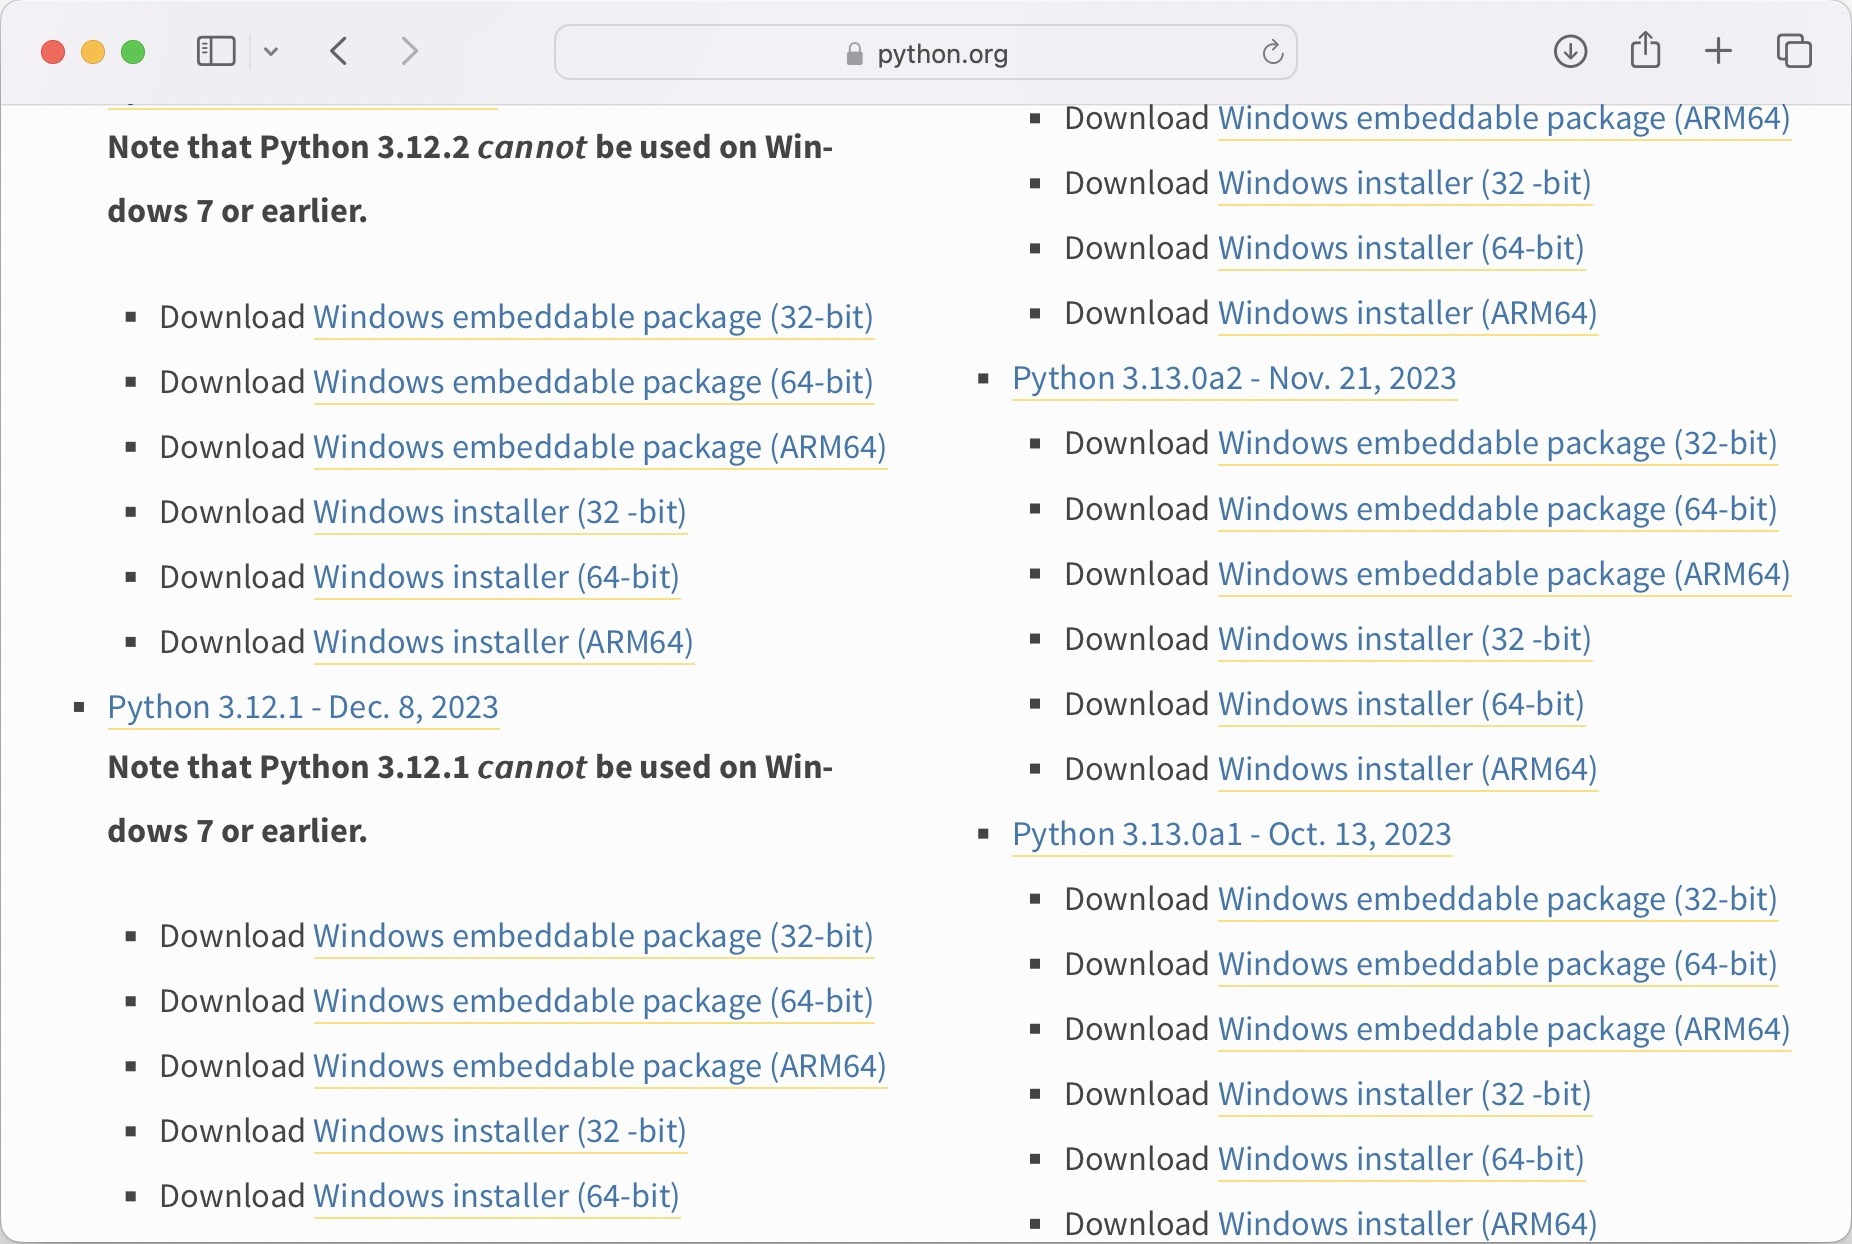
\includegraphics[width=.98\textwidth, trim={2.4mm 2mm 2mm 2mm},clip]{images/vscode_install/2.jpg}};
    \drawshadow{image}
    \draw [draw=red,very thick,rounded corners] (0.5,7) rectangle (6,7.78);
    \draw [draw=red,very thick,rounded corners] (0.75,4.38) rectangle (4.9,4.8);

\end{tikzpicture}
\caption{} 
\label{fig:pyvers}
\end{figure}

ဒေါင်းလုဒ်ပြီးရင် အင်စတော်လာဖိုင်ကို ညာကလစ်နှိပ်ပြီး \mytcboxinl{\fEnSnd{Run as administrator}} လုပ်ပါ။ ပုံ (\fRefNo{\ref{fig:pyinstlrun}}) ကိုကြည့်ပါ။ ပုံ (\fRefNo{\ref{fig:pyinstl1}}) မှာလို ဒိုင်ယာလော့ဂ် ဘောက်စ် ပွင့်လာပါမယ်။ အနီဝိုင်းထားတဲ့ ချက်ခ်ဘောက်စ်နှစ်ခုကို ချက်ခ်လုပ်ပြီး \mytcboxinl{\fEnSnd{Install Now}} နှိပ်ပါ။ အင်စတောလ် ပြီးလို့ \mytcboxinl{\fEnSnd{Setup was successful}} ပေါ်လာရင် \mytcboxinl{\fEnSnd{Close}} ခလုတ်နှိပ်ပြီး ပိတ်ပါ။

ဝင်းဒိုး \fEnSnd{command prompt (cmd)} မှာ \mytcboxinl{\fCode{python --version}} \fEn{run} ရင် ပုံ (\fRefNo{\ref{fig:pycmdchk}}) မှာလို အင်စတောလ်လုပ်ထားတဲ့ ဗားရှင်းကို ပြပေးသင့်ပါတယ်။
\begin{figure}[tbh!]
\begin{tikzpicture}
    \node[anchor=south west,inner sep=0] (image) at (0,0)
        {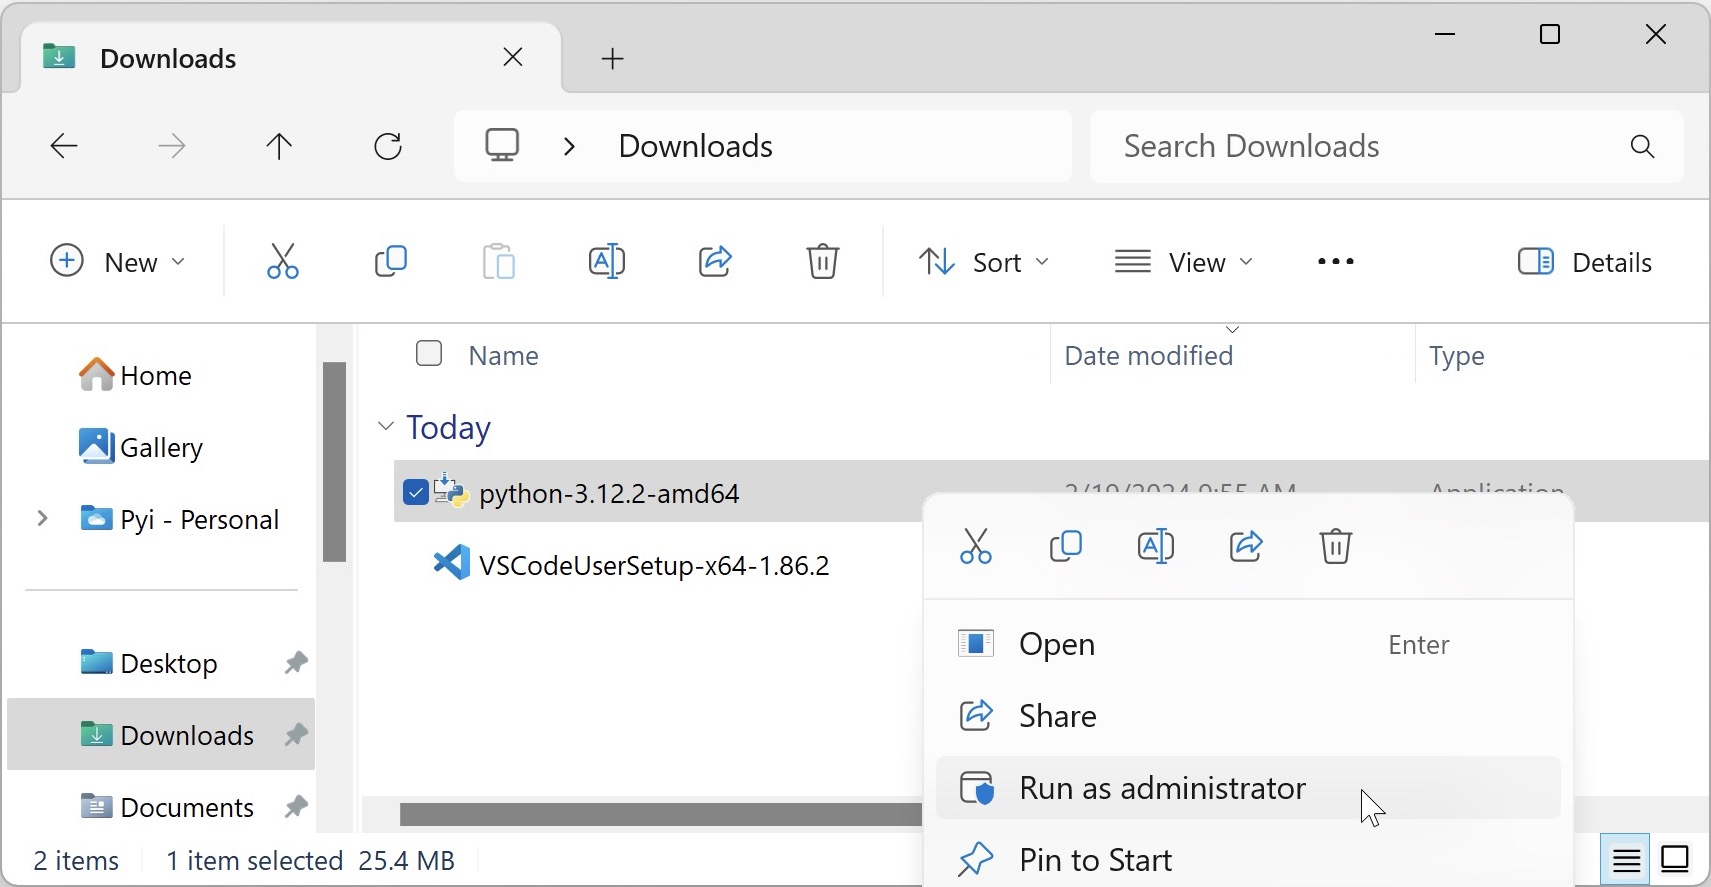
\includegraphics[width=.98\textwidth, trim={2.4mm 2mm 2mm 2mm},clip]{images/vscode_install/3.jpg}};
    \drawshadow{image}
\end{tikzpicture}
\caption{} 
\label{fig:pyinstlrun}
\end{figure}

\begin{figure}[tbh!]
\begin{tikzpicture}
    \node[anchor=south west,inner sep=0] (image) at (0,0)
        {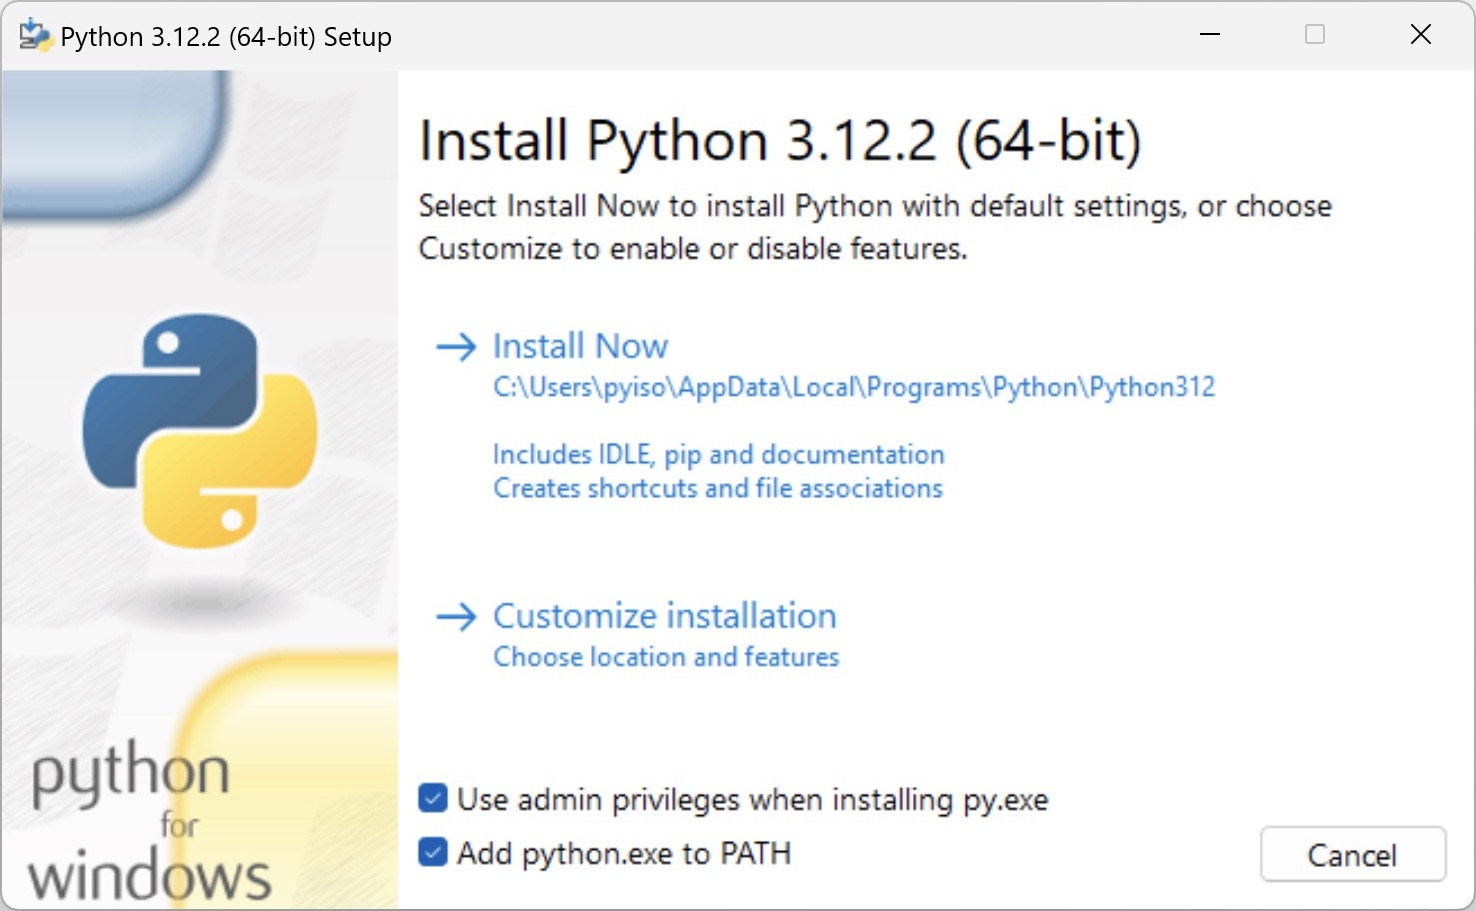
\includegraphics[width=.98\textwidth, trim={2.4mm 2mm 2mm 2mm},clip]{images/vscode_install/4.jpg}};
    \drawshadow{image}
    \draw [draw=red,very thick,rounded corners] (3.5,0.24) rectangle (9.25,1.15);
    \draw [draw=red, thick,rounded corners] (3.73,5.1) rectangle (10.75,4.35);
\end{tikzpicture}
\caption{} 
\label{fig:pyinstl1}
\end{figure}

\begin{figure}[tbh!]
\begin{tikzpicture}
    \node[anchor=south west,inner sep=0] (image) at (0,0)
        {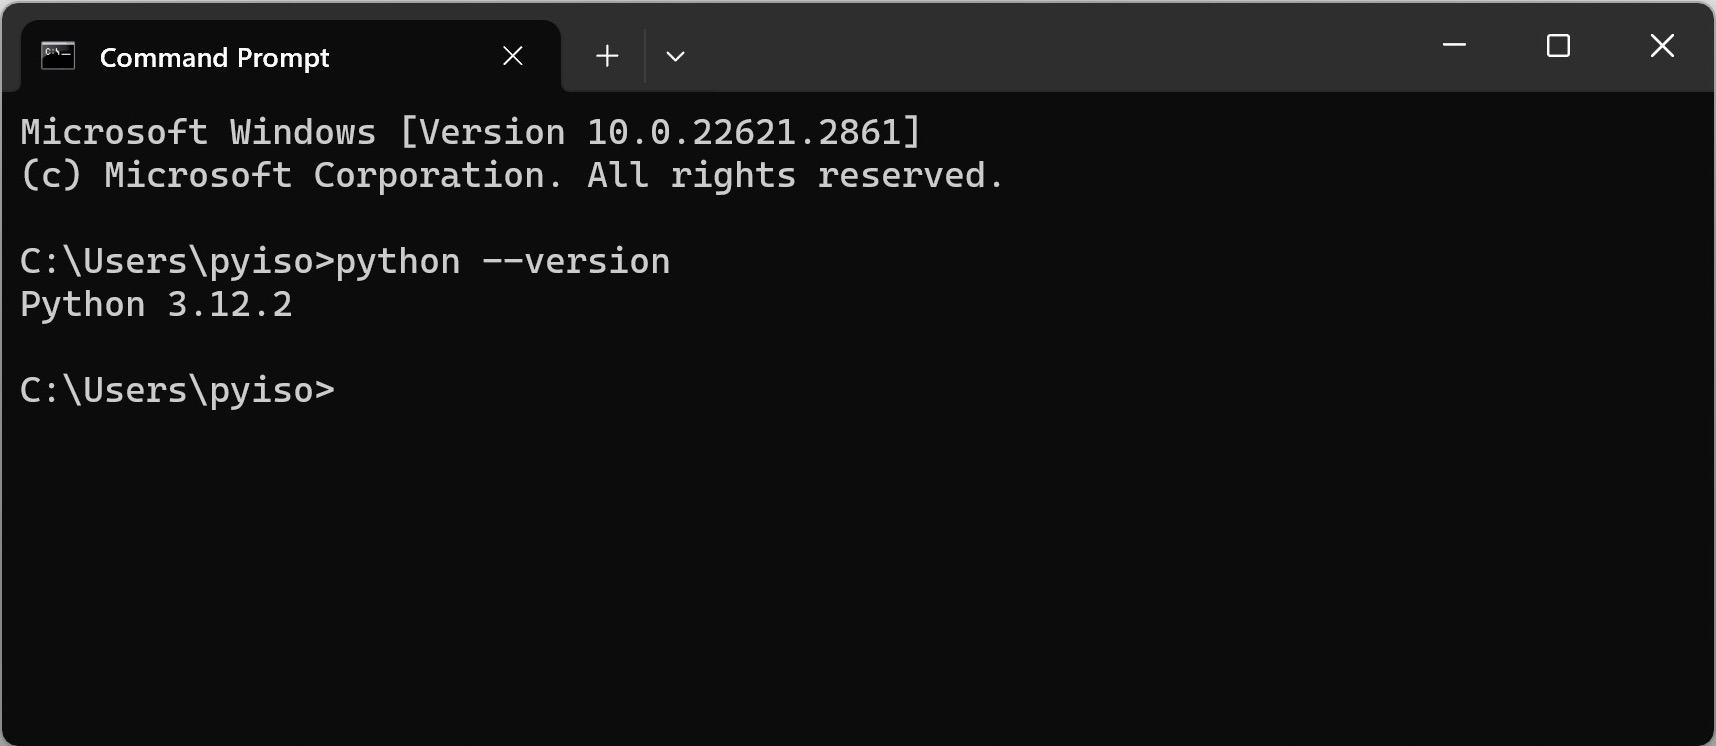
\includegraphics[width=.98\textwidth, trim={2.4mm 2mm 2mm 2mm},clip]{images/vscode_install/5.jpg}};
    \drawshadow{image}
\end{tikzpicture}
\caption{} 
\label{fig:pycmdchk}
\end{figure}

\clearpage
\subsection*{VS Code အင်စတောလ်လုပ်ခြင်း}\label{sec:vscode}
အခုဆိုရင် \fEn{Python programming language} အောင်မြင်စွာ ထည့်ပြီးသွားပါပြီ။ \fEn{VS Code} အင်စတောလ် ဆက်လုပ်ပါမယ်။ အင်စတာ်လာ ဒေါင်းလုဒ်လုပ်ရန် ဝဘ်စာမျက်နှာကို အောက်ပါလင့်
%
\begin{minted}[frame=lines, framerule=0pt]{text}
https://code.visualstudio.com 
\end{minted}
%
မှတစ်ဆင့် သွားပါ။ ပုံ (\fRefNo{\ref{fig:vsdwnpg}}) ဝဘ်စာမျက်နှာကို တွေ့ရပါမယ်။ \mytcboxinl{\fEnSnd{Download for Windows}} နှိပ်၍ ဒေါင်းလုဒ်လုပ်ပါ။

ပြီးတဲ့အခါ အင်စတော်လာဖိုင်ကို ညာကလစ်နှိပ်ပြီး ဖွင့်ပါ (ပုံ \fRefNo{\ref{fig:vsinstlropn}} မှာ ပြထားပါတယ်)။ အင်စတောလ် ဒိုင်ယာလော့ဂ်ဘောက်စ် ပွင့်လာရင် \mytcboxinl{\fEnSnd{I accept the agreement}} ကို ချက်ခ်လုပ်၍ \fEnSnd{Next>} တစ်ခုပြီးတစ်ခု ဆက်နှိပ်သွားပြီး နောက်ဆုံးမှာ  \fEnSnd{Install} နှိပ်ပါ။ အင်စတောလ်လုပ်နေတာကို ခဏစောင့်ပြီး၊ ပြီးသွားရင် \fEnSnd{Finish} နှိပ်ပါ။  

\fEn{Welcome} စခရင်ကို ပုံ (\fRefNo{\ref{fig:vswlcm}}) လို တွေ့ရပါမယ်။ \mytcboxinl{\fEnSnd{Dark Modern}} (သို့) \mytcboxinl{\fEnSnd{Light Modern}} နှစ်သက်ရာ သီးမ်စ် ရွေးပါ။ ဒါဆိုရင် \fEn{VS Code} လည်း အင်စတောလ် လုပ်ပြီးသွားပါပြီ။ ကားရဲလ်ပရိုဂရမ် ရေးဖို့ ဆက်လုပ်ရပါမယ်။

\begin{figure}[tbh!]
\begin{tikzpicture}
    \node[anchor=south west,inner sep=0] (image) at (0,0)
        {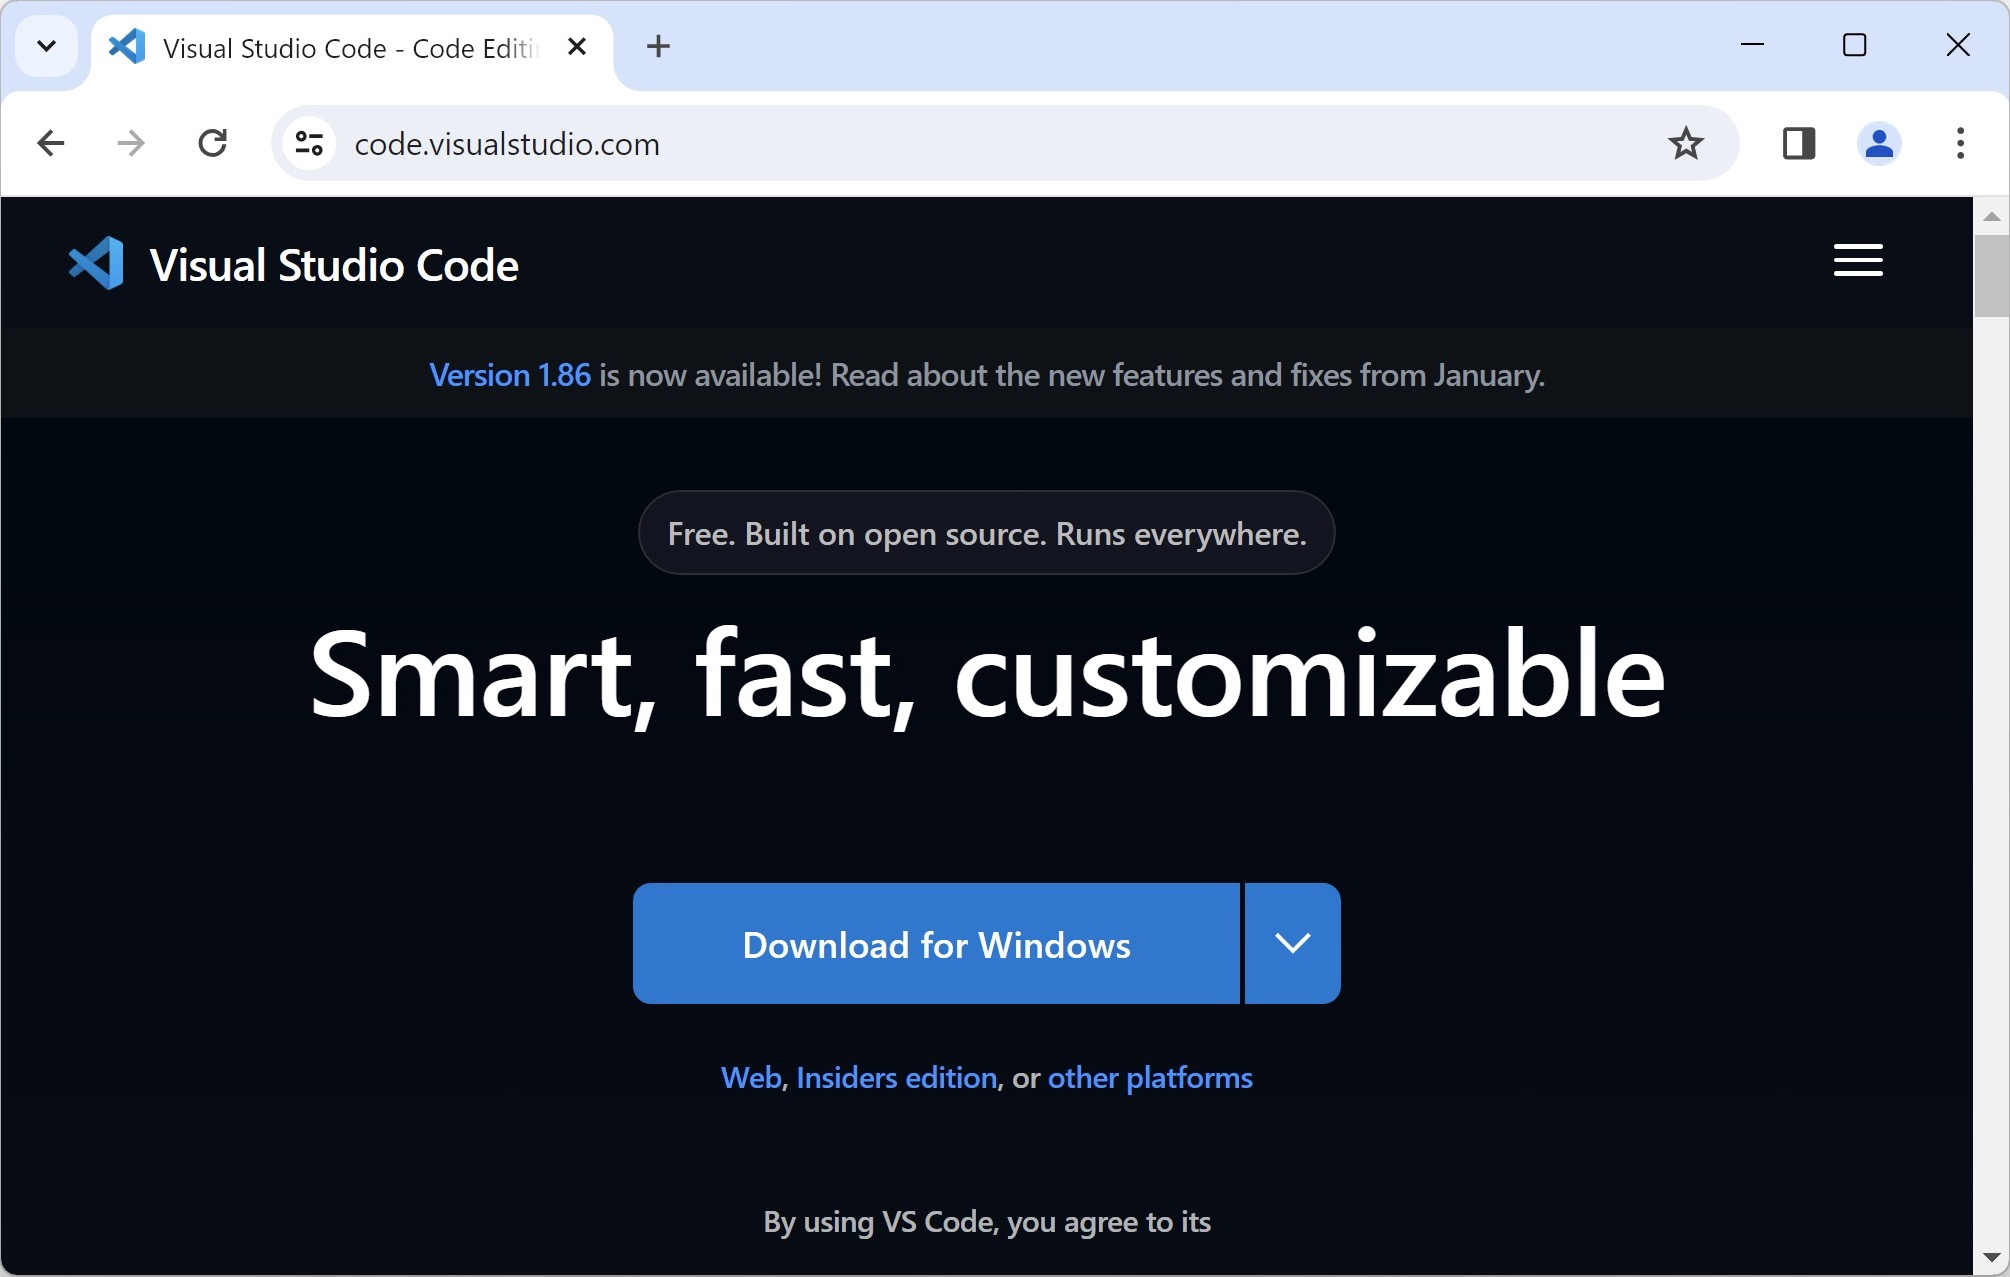
\includegraphics[width=.98\textwidth, trim={2.4mm 2cm 2mm 2mm},clip]{images/vscode_install/v0.jpg}};
    \drawshadow{image}
\end{tikzpicture}
\caption{} 
\label{fig:vsdwnpg}
\end{figure}

\begin{figure}[tbh!]
\begin{tikzpicture}
    \node[anchor=south west,inner sep=0] (image) at (0,0)
        {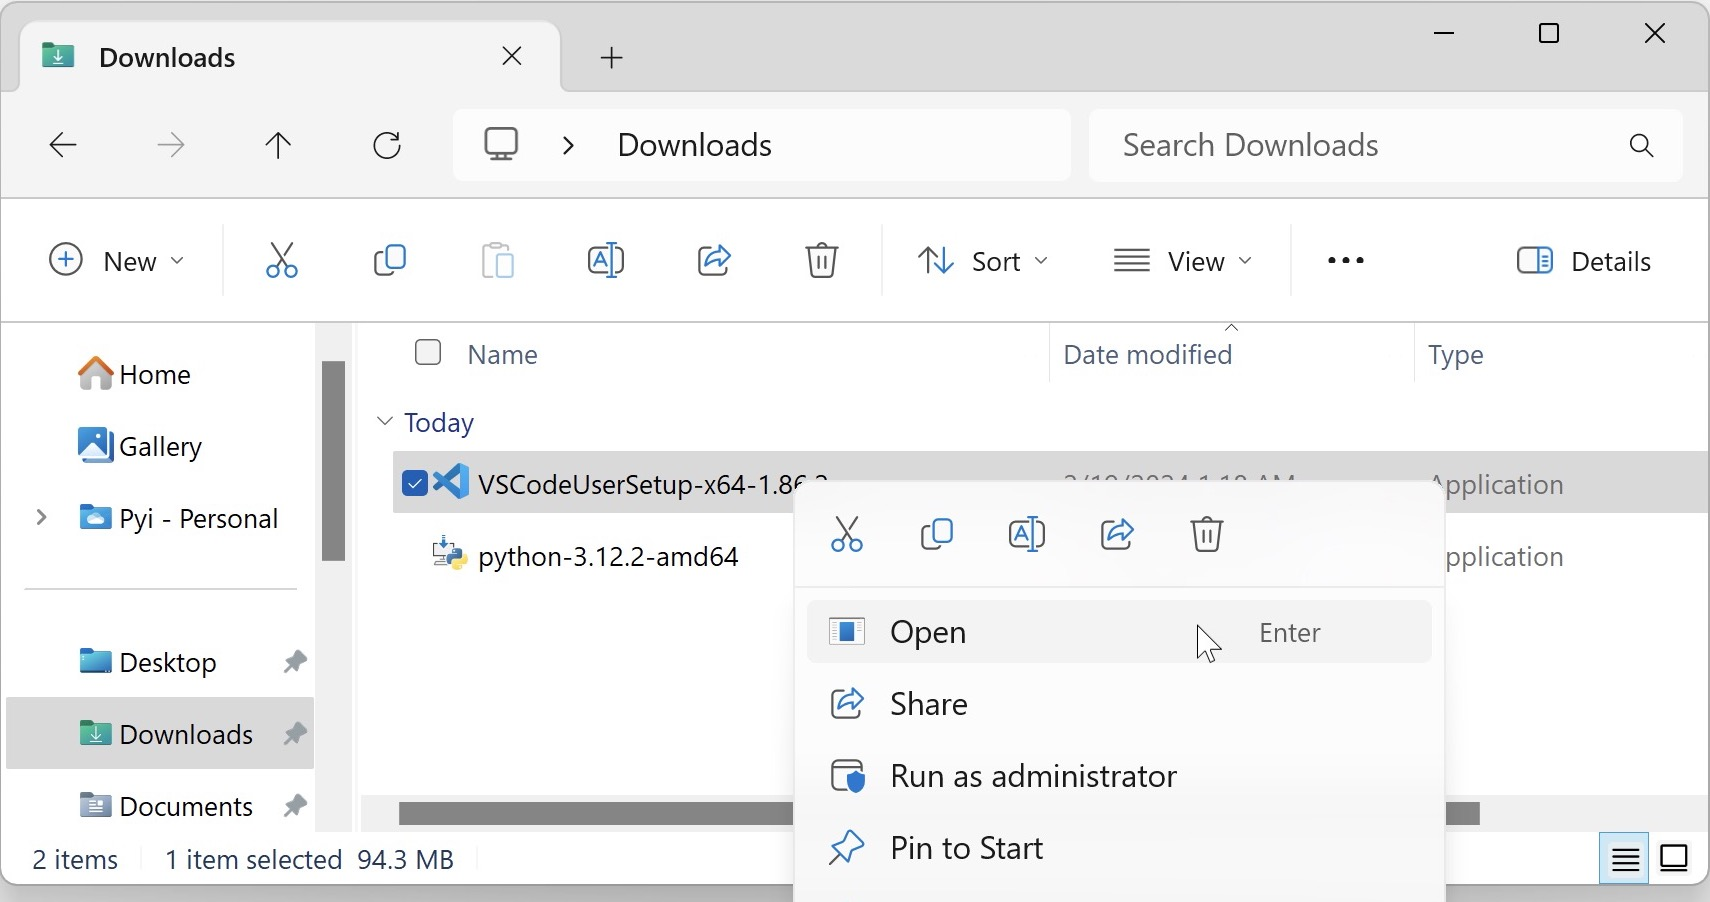
\includegraphics[width=.98\textwidth, trim={2.4mm 2mm 2mm 2mm},clip]{images/vscode_install/v1.jpg}};
    \drawshadow{image}
\end{tikzpicture}
\caption{} 
\label{fig:vsinstlropn}
\end{figure}

\begin{figure}[tbh!]
\begin{tikzpicture}
    \node[anchor=south west,inner sep=0] (image) at (0,0)
        {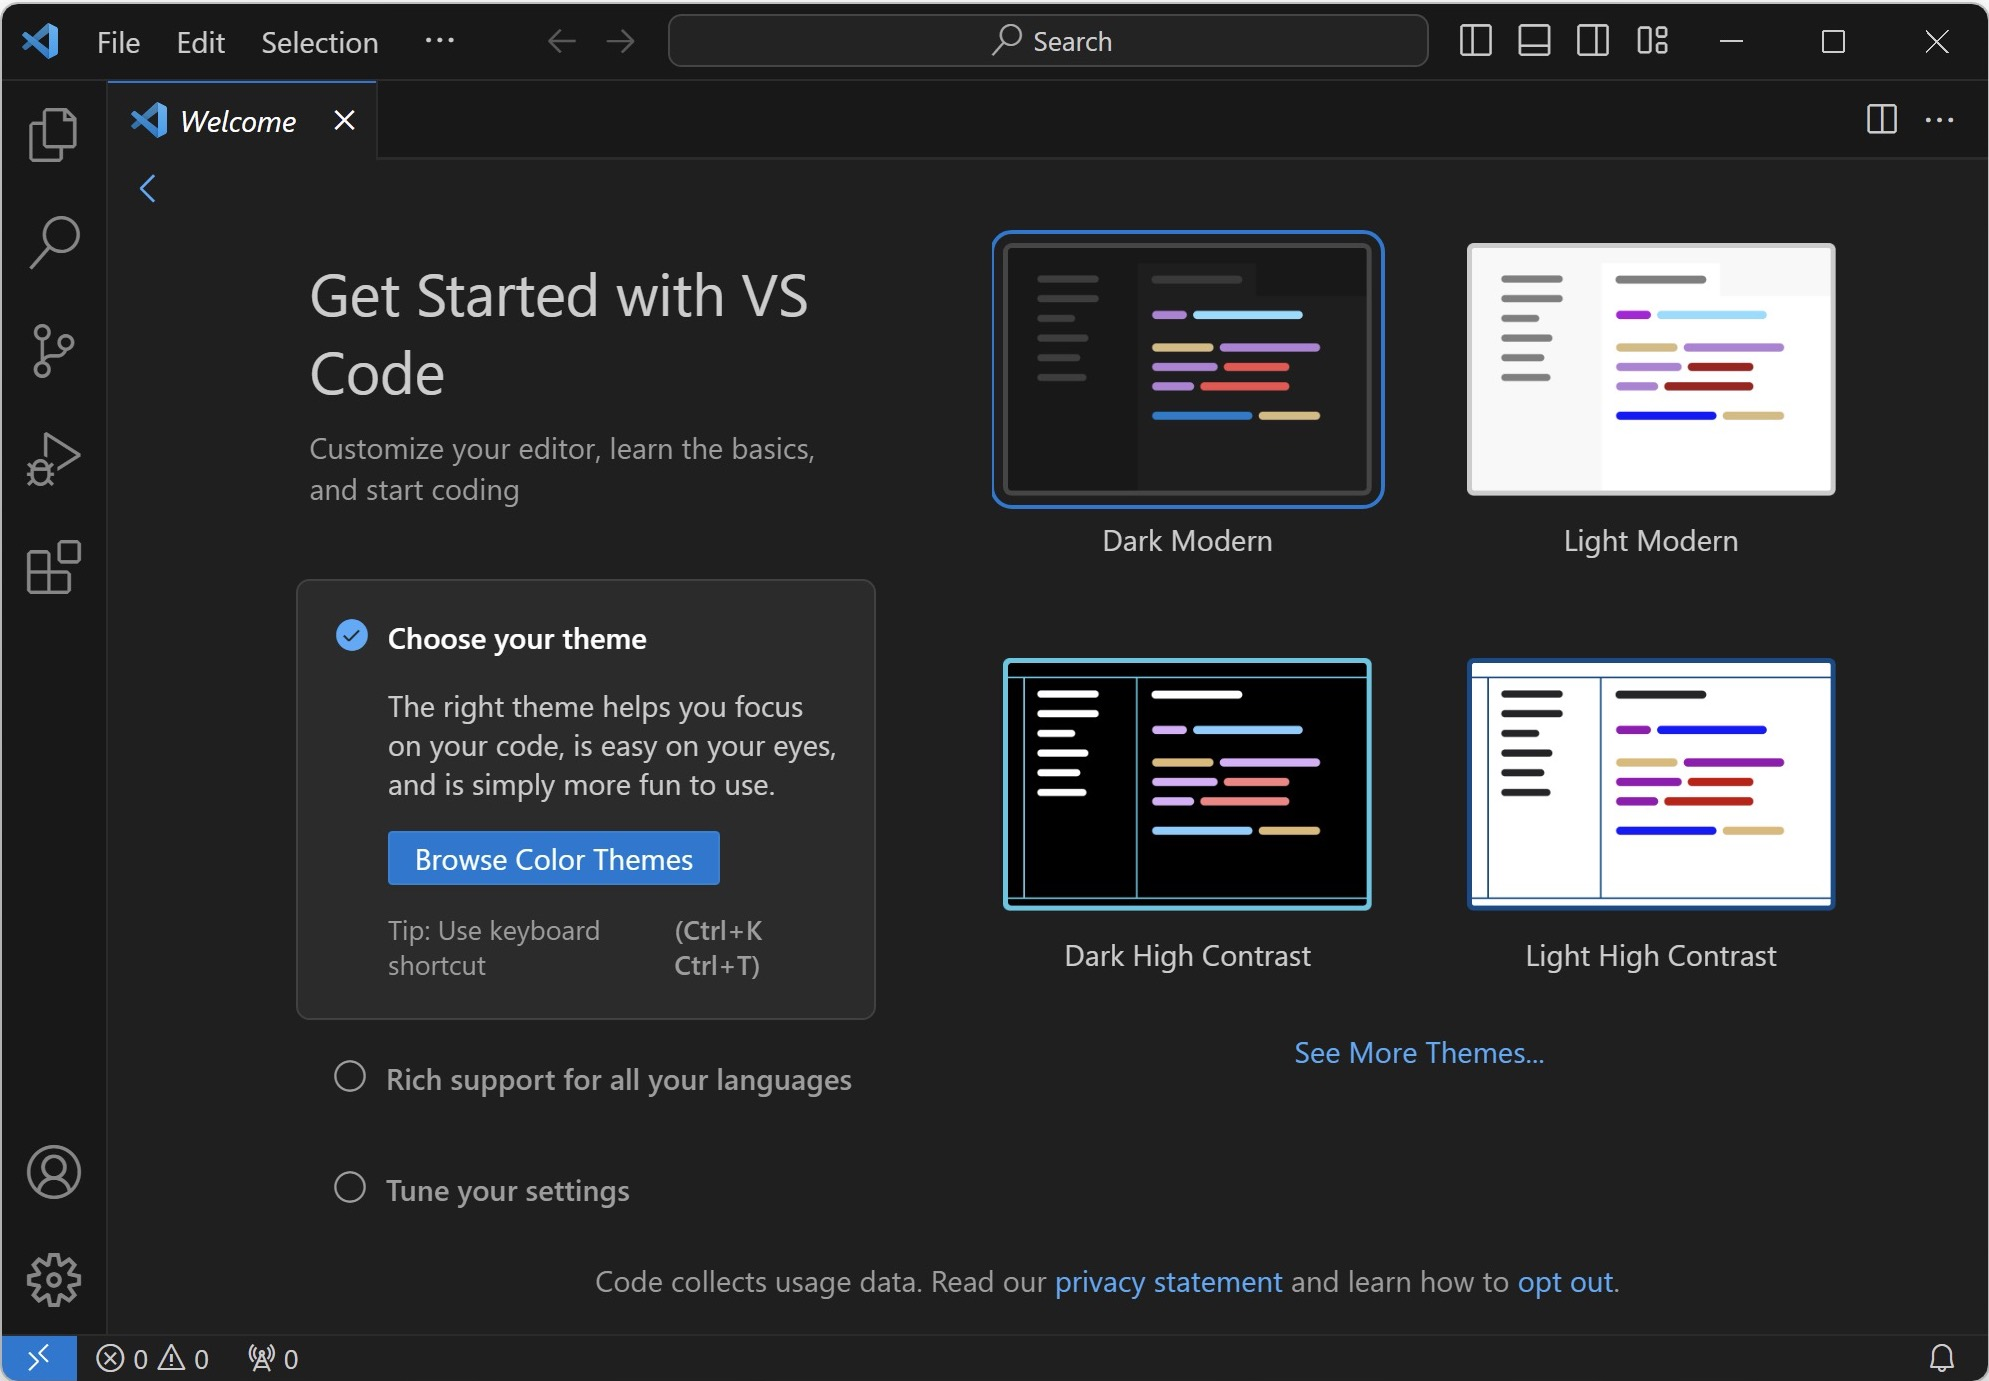
\includegraphics[width=.98\textwidth, trim={2.4mm 2mm 2mm 2mm},clip]{images/vscode_install/v1b.jpg}};
    \drawshadow{image}
    
    \draw [draw=red,very thick,rounded corners] (6.25,7.5) rectangle (9.08,5.25);
    \draw [draw=red,very thick,rounded corners] (9.35,7.5) rectangle (12.01,5.25);
    \draw [draw=red,very thick,rounded corners] (0.08,5.5) rectangle (0.6,5);
\end{tikzpicture}
\caption{} 
\label{fig:vswlcm}
\end{figure}

\clearpage

\subsection*{VS Code Python Extension ထည့်ခြင်း}
\fEn{Python} ပရိုဂရမ်ရေးဖို့အတွက် \fEn{VS Code} က ဒီအတိုင်းဆိုရင် သိပ်အဆင်မပြေသေးပါဘူး။ \fEn{Python} အတွက် \fEn{extension} အင်စတောလ် လုပ်ပေးရပါအုံးမယ်။ ပုံ (\fRefNo{\ref{fig:vswlcm}}) ဘယ်ဘက်ဘောင်နားမှာ အနီဝိုင်းထားတဲ့ အိုင်ကွန်လေးကို နှိပ်ပါ။ \fEn{Python} \fEnSnd{extension} ကိုရှာပါ။   ပုံ (\fRefNo{\ref{fig:vspyplugin1}}) မှာ ဘယ်လိုရှာရမလဲ ပြထားပါတယ်။ ပုံမှာတွေ့ရတဲ့ \fEn{Microsoft} က ထုတ်တဲ့ \fEnSnd{extension} ကို အင်စတောလ်လုပ်ပါ။ အောင်မြင်ရင် ပုံ (\fRefNo{\ref{fig:vspyplugin2}}) မှာလို ဖြစ်သွားပါမယ်။ \fEn{Python} နဲ့  \fEn{VS Code} ကိစ္စတော့ ပြီးသွားပြီ။ ကားရဲလ် \fEn{example} \fEn{run} ဖို့ ဆက်လုပ်ရမယ်။
\begin{figure}[tbh!]
\begin{tikzpicture}
    \node[anchor=south west,inner sep=0] (image) at (0,0)
        {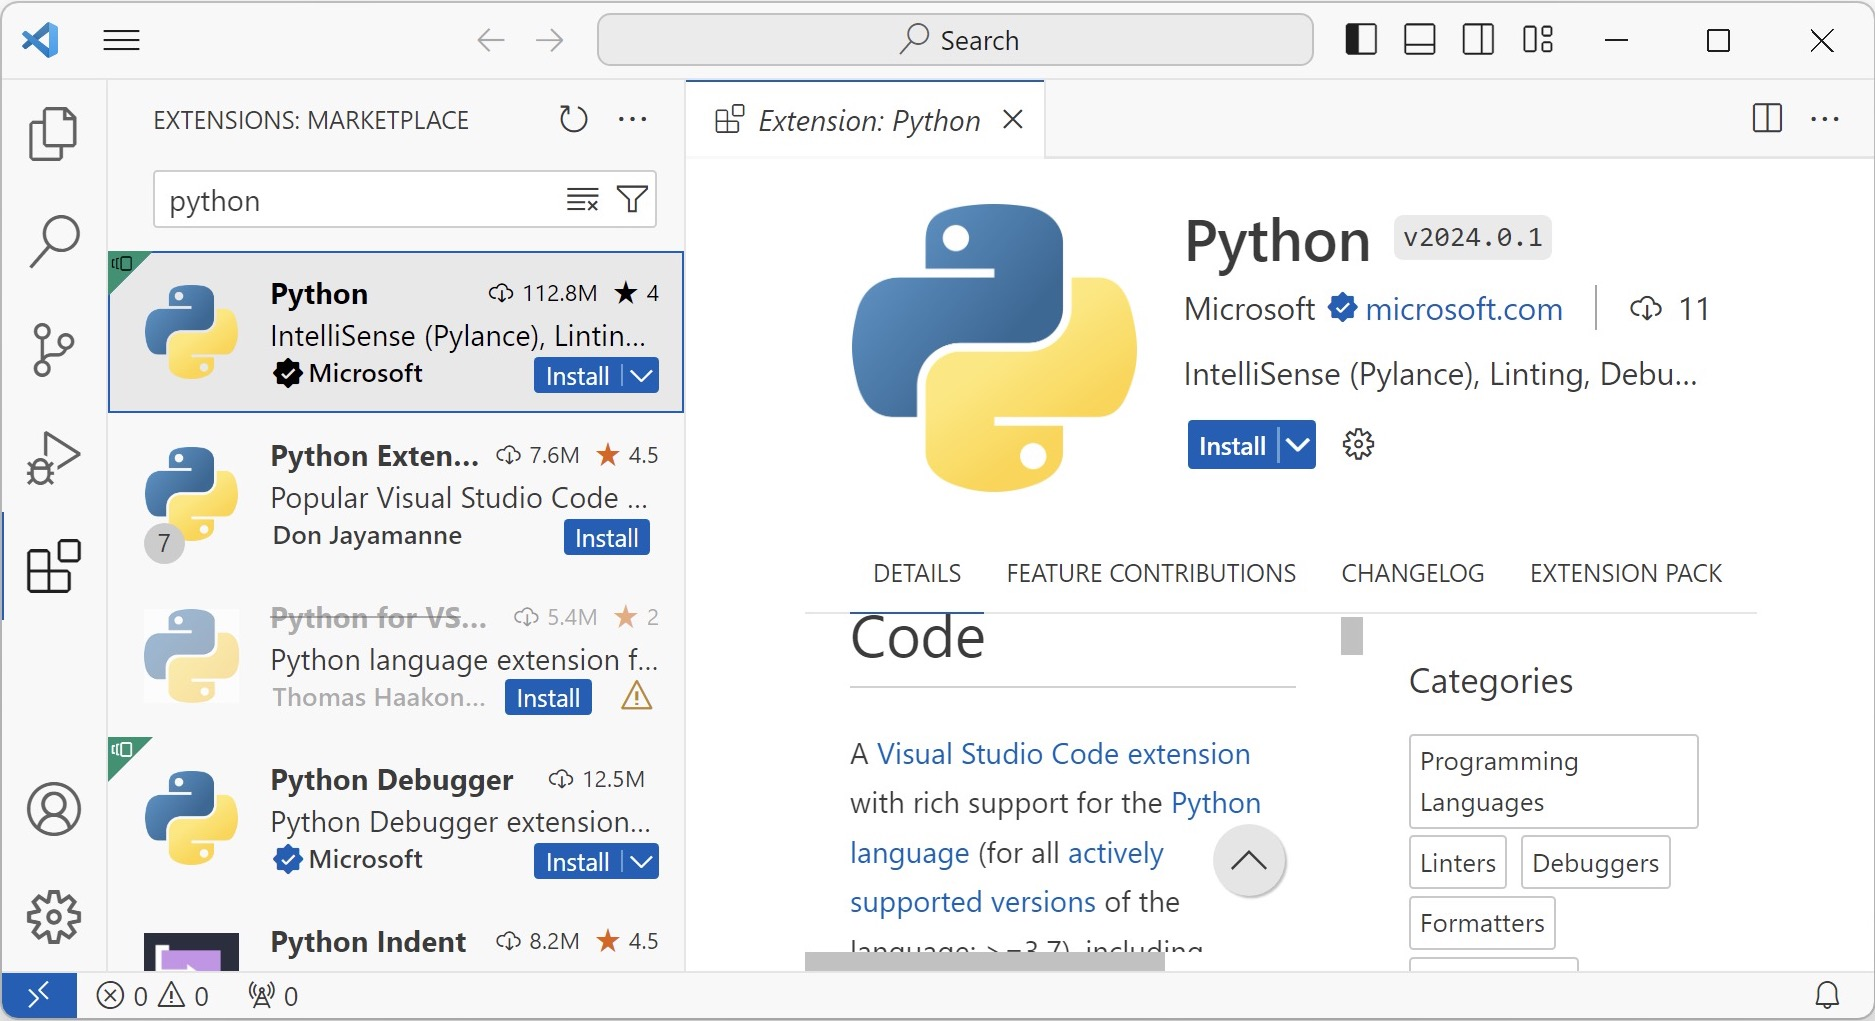
\includegraphics[width=.98\textwidth, trim={2.4mm 2mm 2mm 2mm},clip]{images/vscode_install/v2.jpg}};
    \drawshadow{image}
\end{tikzpicture}
\caption{} 
\label{fig:vspyplugin1}
\end{figure}

\begin{figure}[tbh!]
\begin{tikzpicture}
    \node[anchor=south west,inner sep=0] (image) at (0,0)
        {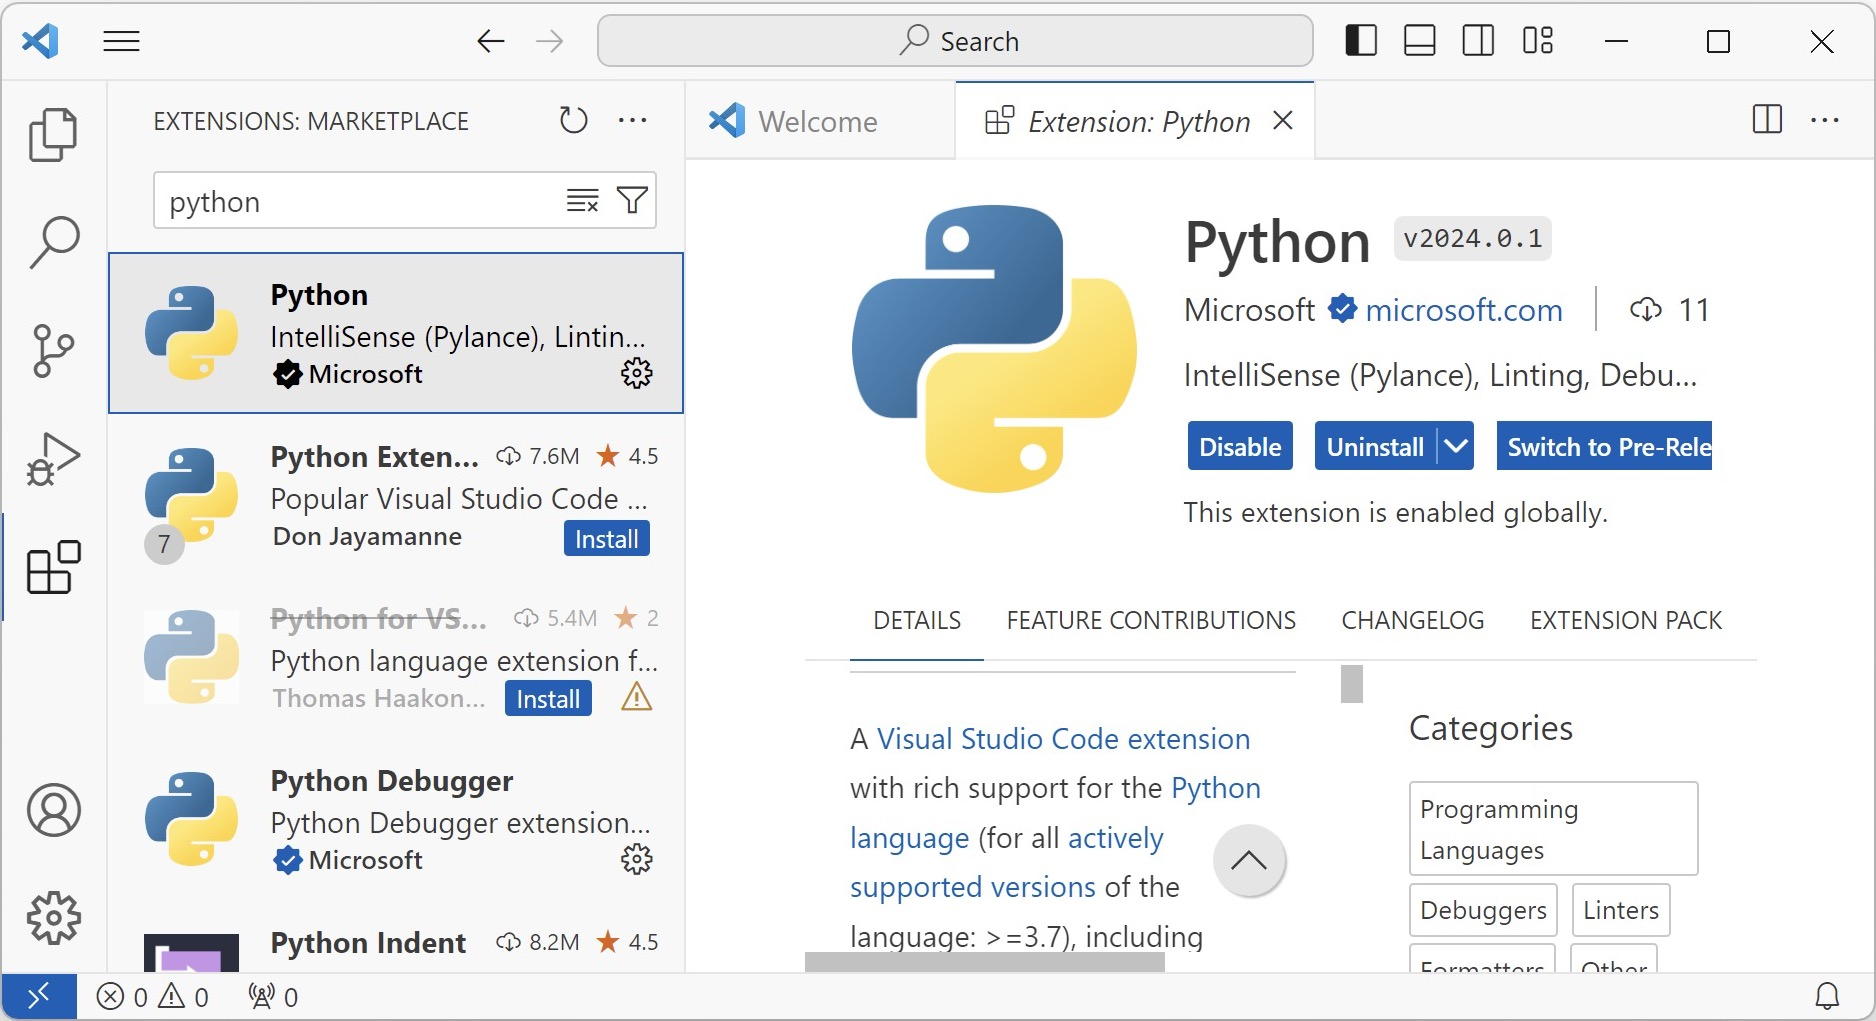
\includegraphics[width=.98\textwidth, trim={2.4mm 2mm 2mm 2mm},clip]{images/vscode_install/v3.jpg}};
    \drawshadow{image}
\end{tikzpicture}
\caption{} 
\label{fig:vspyplugin2}
\end{figure}

\clearpage

\subsection*{နမူနာ ကားရဲလ် ကမ္ဘာနှင့် ပရိုဂရမ်ကုဒ် ဖိုင်များထည့်ခြင်း}
\fEnSnd{meet\_karel.zip} ဖိုင်ကို \todo{ဒေါင်းလုဒ်လင့်ထည့်ရန်} ဒီလင့် \fCode{http://tinyurl.com/3mmm9c7j} ကနေ ဒေါင်းလုဒ်လုပ်ပါ။ ၎င်း \fEnSnd{zip} ဖိုင်ကို \fEn{extract} လုပ်ပါ။ \fEnSnd{meet\_karel} နံမည်နဲ့ ဖိုဒါတစ်ခု ရလာပါမယ်။ ဖိုဒါထဲ ဝင်ကြည့်ရင် အောက်ပါအတိုင်း ရှိသင့်ပါတယ်။ 
%
\begin{itemize}
    \item \fEnSnd{worlds} 
    \begin{itemize}
        \item \fEnSnd{meet\_karel.w}
        \item \fEnSnd{move\_beeper\_to\_other\_side.w}
    \end{itemize}
    \item \fEnSnd{meet\_karel.py}
    \item \fEnSnd{move\_beeper\_to\_other\_side.py}
    \item \fEnSnd{world\_editor.py}
\end{itemize}
%

\begin{figure}[tbh!]
\begin{tikzpicture}
    \node[anchor=south west,inner sep=0] (image) at (0,0)
        {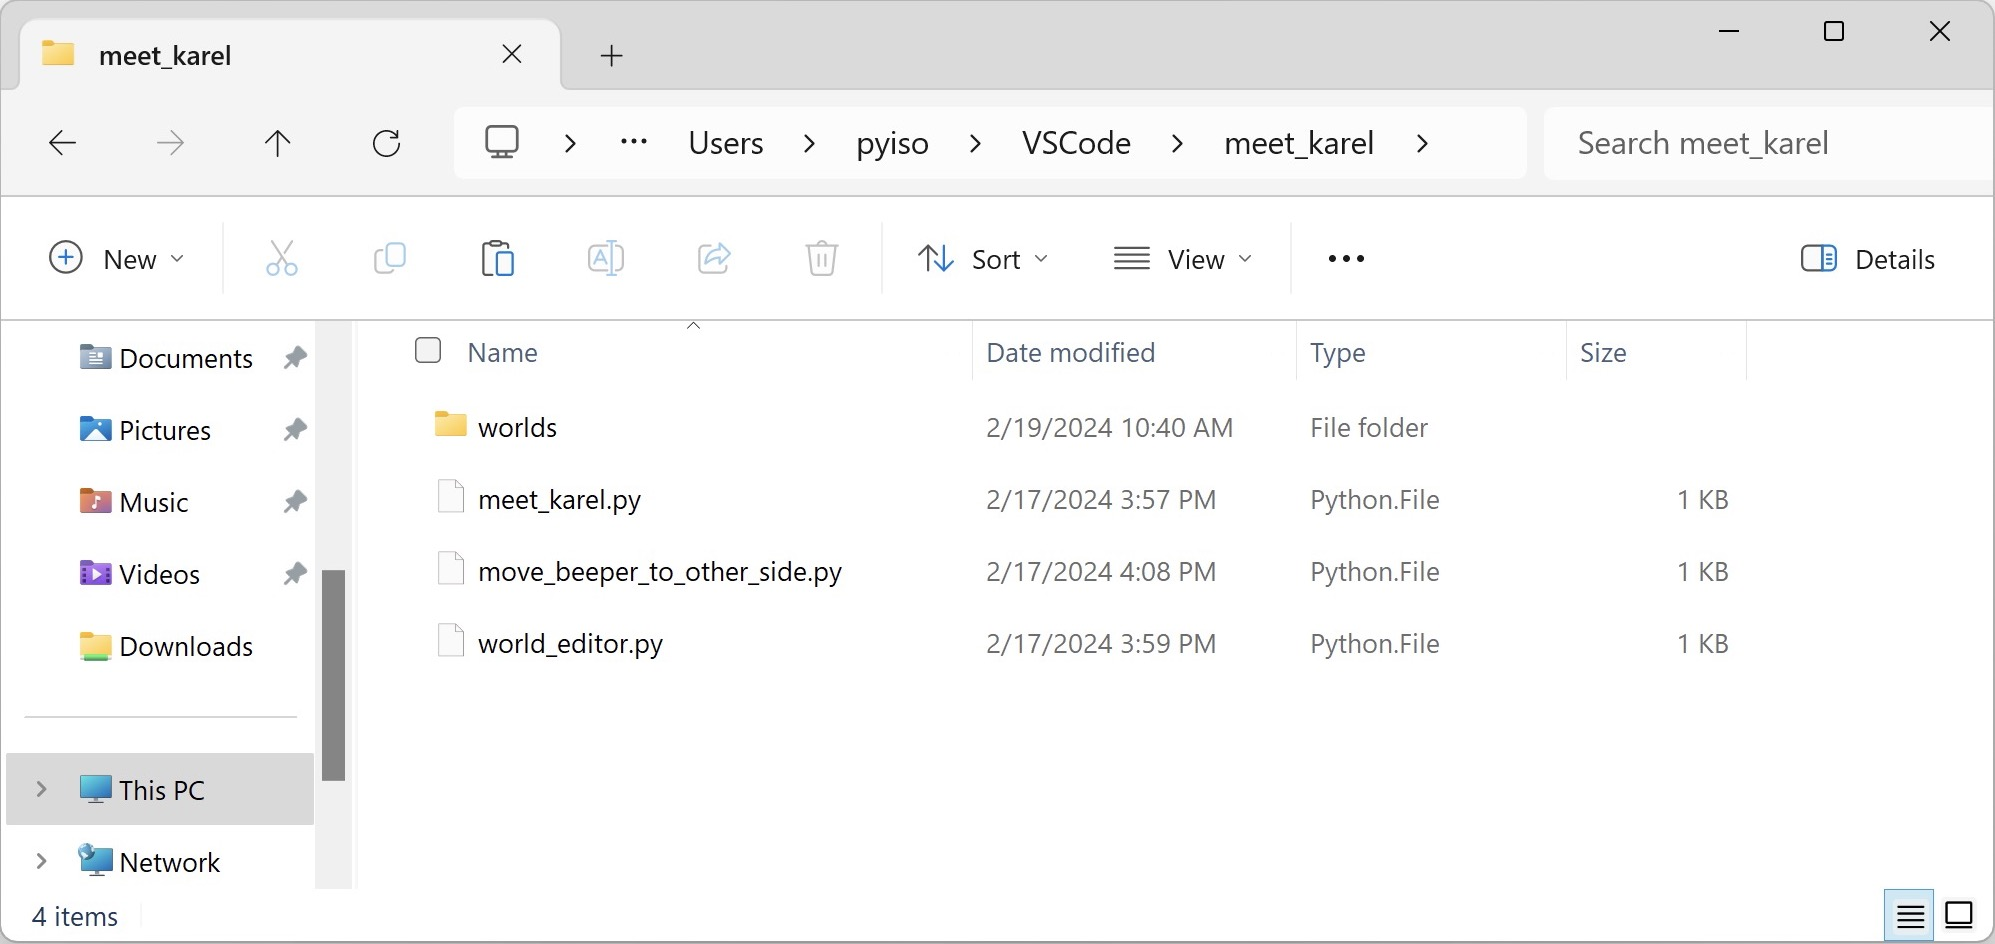
\includegraphics[width=.98\textwidth, trim={2.4mm 2mm 2mm 2mm},clip]{images/vscode_install/v4.jpg}};
    \drawshadow{image}
\end{tikzpicture}
\caption{} 
\label{fig:mtkrl1}
\end{figure}

\begin{figure}[tbh!]
\begin{tikzpicture}
    \node[anchor=south west,inner sep=0] (image) at (0,0)
        {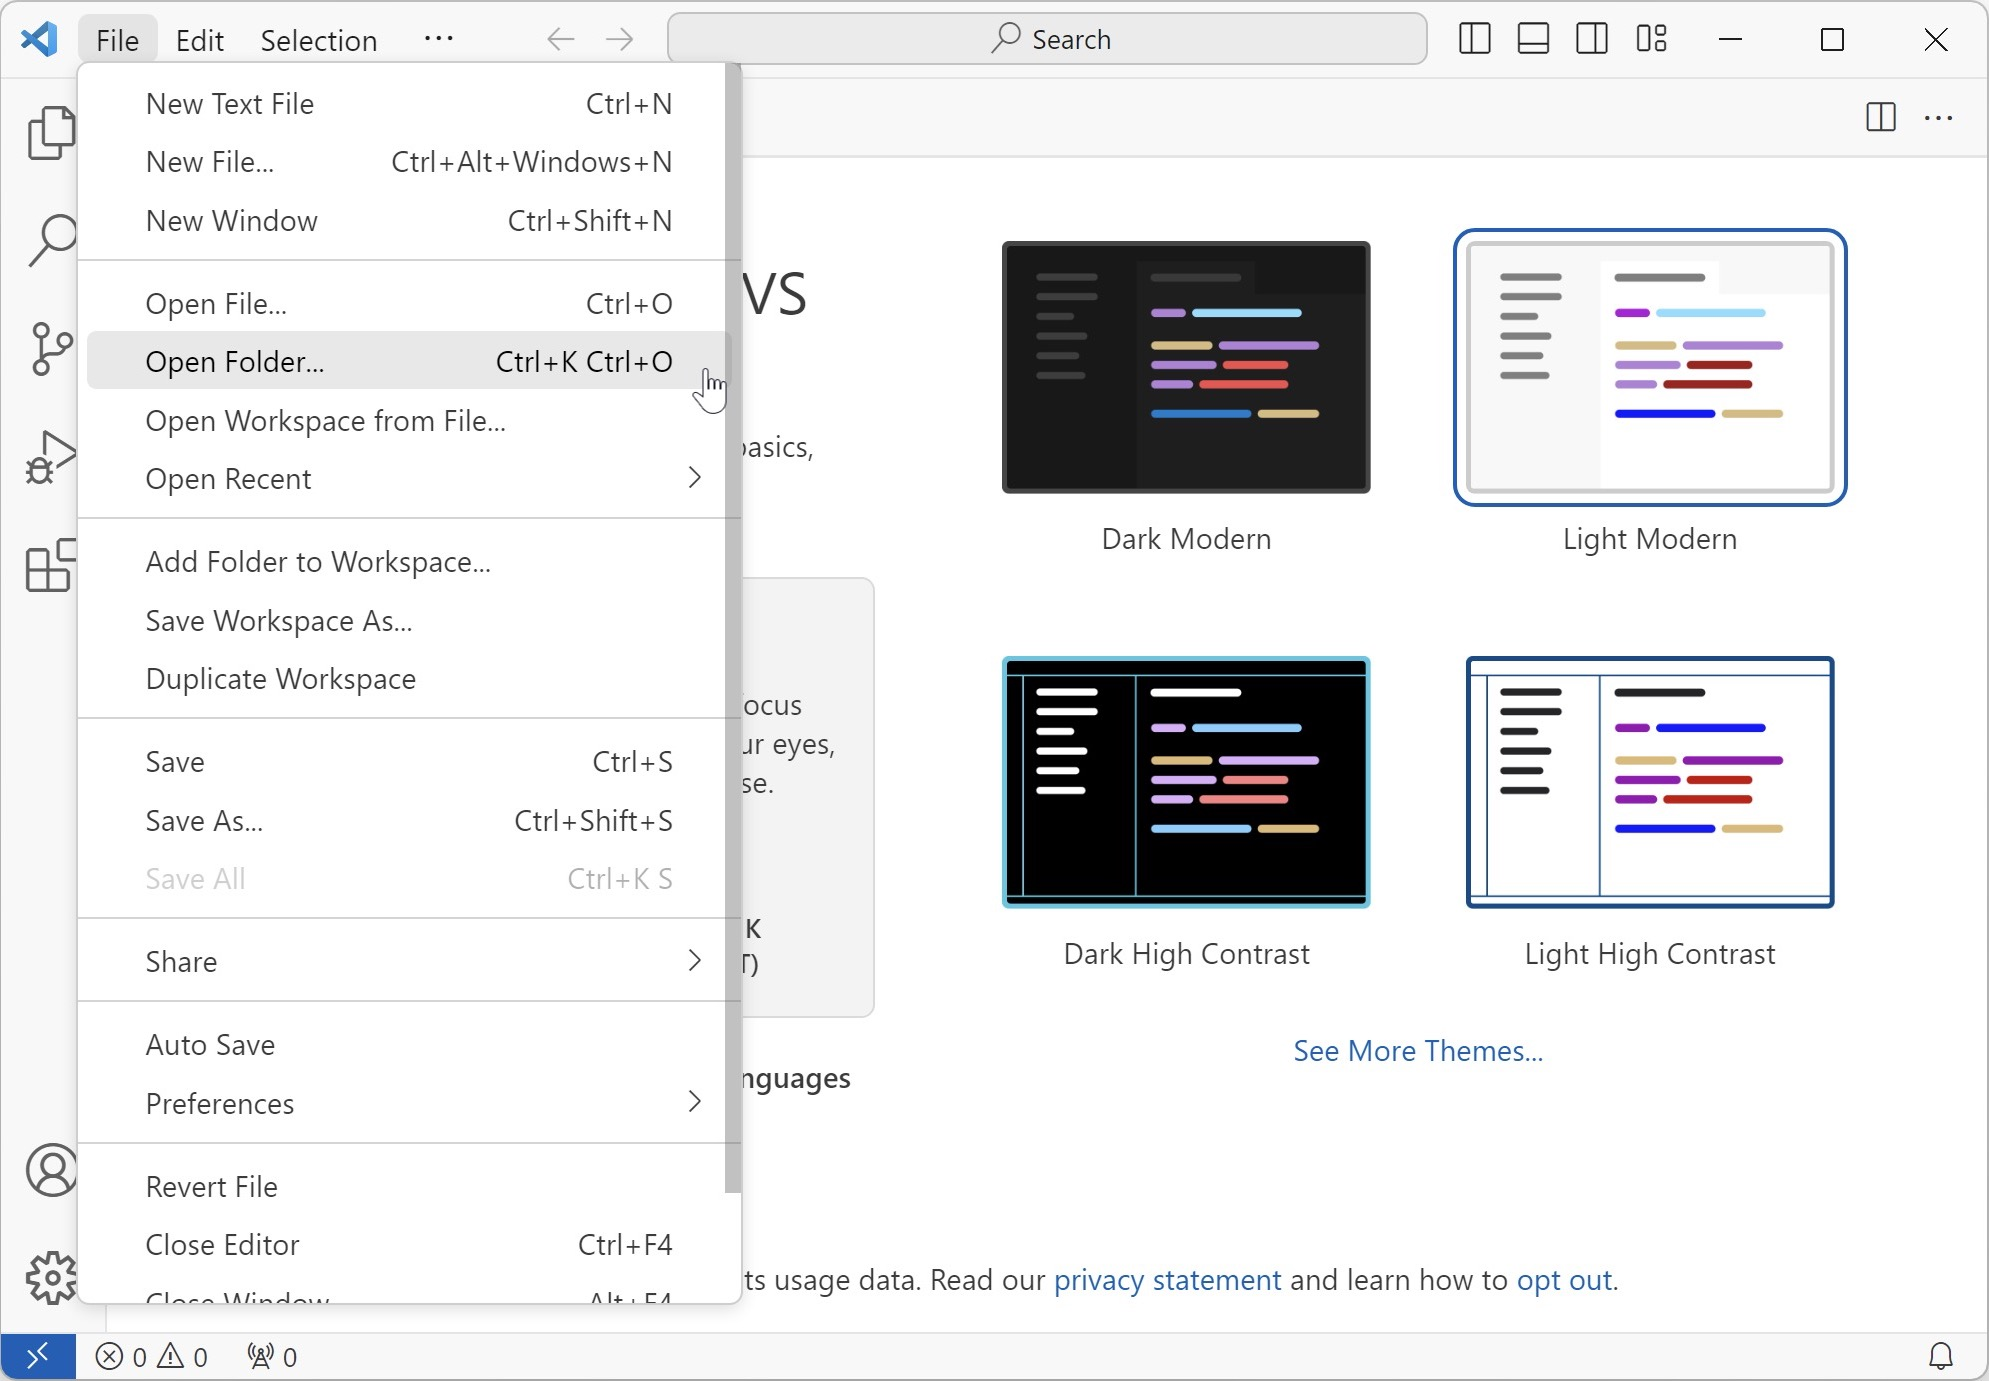
\includegraphics[width=.98\textwidth, trim={2.4mm 2mm 2mm 2mm},clip]{images/vscode_install/v5b.jpg}};
    \drawshadow{image}
\end{tikzpicture}
\caption{} 
\label{fig:opnmtkrl}
\end{figure}

\begin{figure}[tbh!]
\begin{tikzpicture}
    \node[anchor=south west,inner sep=0] (image) at (0,0)
        {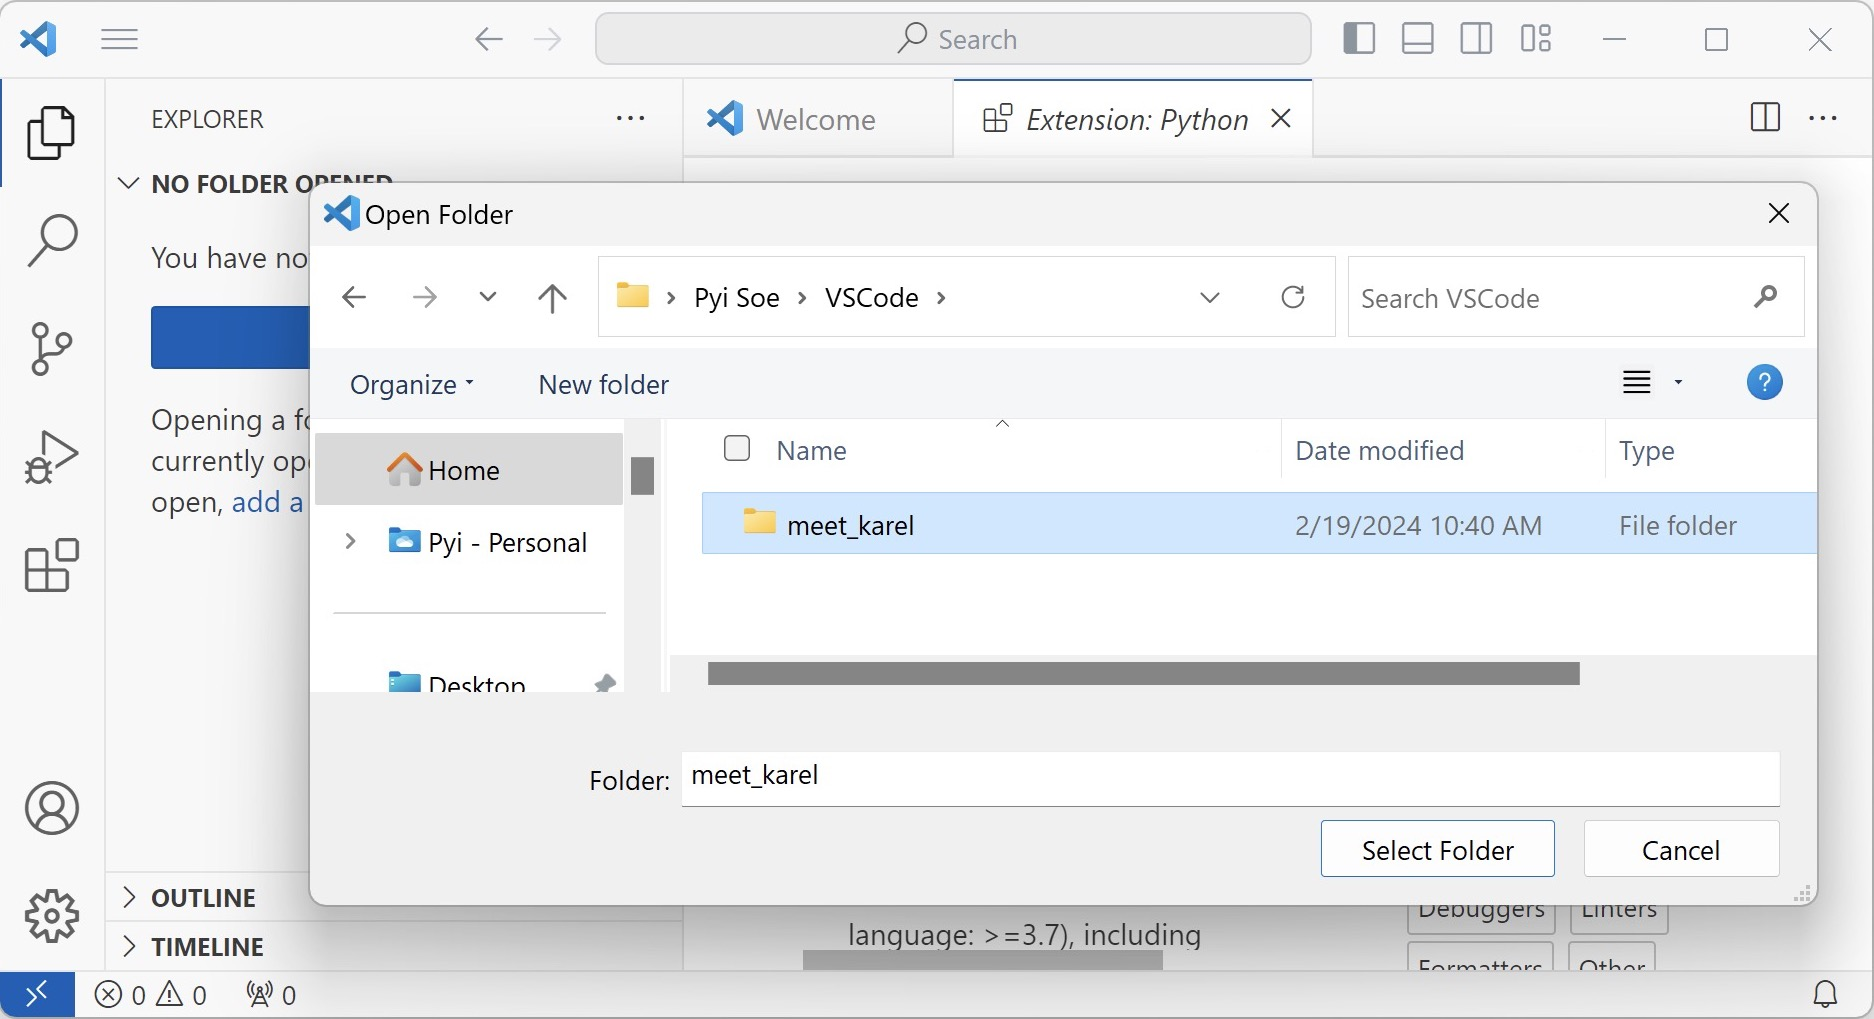
\includegraphics[width=.98\textwidth, trim={2.4mm 2mm 2mm 2mm},clip]{images/vscode_install/v6.jpg}};
    \drawshadow{image}
\end{tikzpicture}
\caption{} 
\label{fig:mtkrl3}
\end{figure}

\fEn{VS Code} အတွက် ဖိုဒါတစ်ခုကို မိမိအတွက် အဆင်ပြေမဲ့နေရာမှာ သီးသန့်တည်ဆောက် ထားသင့်တယ်။ ဥပမာ 
%
\begin{minted}[frame=lines, framerule=0pt,escapeinside=ßß]{text}
ß\fEnSnd{C:{\textbackslash}Users{\textbackslash}\textit{yourname}{\textbackslash}VS Code}ß
\end{minted}
%
\begin{mytcbox}
မိမိ လက်ရှိ \fEn{Home} ဖိုဒါကို  \mytcboxinl{\fEnSnd{C:}} \fEn{drive} ရဲ့ \mytcboxinl{\fEnSnd{Users}}  ဖိုဒါထဲမှာ တွေ့နိုင်ပါတယ်။ \mytcboxinl{\fEnSnd{Win + R}} ရှော့ကတ်နှိပ်ပြီး \mintinline{text}|%userprofile%| ရိုက်ထည့်၊ \fEnSnd{Ok} လုပ်ပြီး \fEn{Home} ဖိုဒါကို သွားနိုင်ပါတယ်။ အကယ်၍ မသွားတတ်ရင်လည်း ပြဿနာမရှိပါဘူး။ ကိုယ့်အတွက် လွယ်ကူမဲ့ \fEnSnd{Desktop, Downloads, Documents} တစ်ခုခုထဲမှာ \fEn{VS Code} အတွက် ဖိုဒါတစ်ခု ထားလည်းရတယ်။
\end{mytcbox}

\mytcboxinl{\fEnSnd{meet\_karel}} ဖိုဒါ (\fEnSnd{.zip} ဖိုင်မဟုတ်ပါ) ကို အထက်ပါအတိုင်း အသစ် ဆောက်ထားတဲ့ \fEn{VS Code} သီးသန့်ဖိုဒါထဲကို ကော်ပီကူးထည့်ပါ။ ၎င်း \mytcboxinl{\fEnSnd{meet\_karel}} ဖိုဒါကို \fEn{VS Code} \mytcboxinl{\fEnSnd{File}} မီနူးမှ \mytcboxinl{\fEnSnd{Open Folder}} နှိပ်၍ ဖွင့်ပါ။ ပုံ (\fRefNo{\ref{fig:opnmtkrl}}) တွင်ကြည့်ပါ။

အခန်းအလိုက် နမူနာ ကုဒ်ဖိုင်တွေ ထည့်ပေးထားတဲ့ \fEnSnd{.zip} ဖိုင်တွေကိုလည်း အထက်ပါအတိုင်း လုပ်ရပါမယ်။ \fEnSnd{.zip} ဖိုင်ကို ဖြည်၊ ရလာတဲ့ ဖိုဒါကို သီးသန့်ဖိုဒါတစ်ခုထဲကို ကော်ပီကူးထည့်၊ \fEn{VS Code} နဲ့ အဲ့ဒီဖိုဒါကို ဖွင့်ရုံပါပဲ။



\clearpage
\subsection*{stanfordkarel လိုက်ဘရီ အင်စတောလ်လုပ်ခြင်း}
\mytcboxinl{\fEnSnd{meet\_karel.py}} ဖိုင်ကို ကလစ်နှစ်ချက်နှိပ် ဖွင့်ပါ။ ကုဒ်အယ်ဒီတာ ပွင့်လာမယ် (ပုံ \fRefNo{\ref{fig:edtmtkrl}})။ အဲဒီ ကုဒ်အယ်ဒီတာပေါ် (သို့) \mytcboxinl{\fEnSnd{meet\_karel.py}} ဖိုင်ကို ညာကလစ်နှိပ်ပြီး \mytcboxinl{\fEnSnd{Run Python File in Terminal}} လုပ်ပါ (ပုံ \fRefNo{\ref{fig:runmtkrl2}})။ \fEnSnd{Terminal} ပွင့်လာပြီး အယ်ရာ\fOpn{မက်ဆေ့ချ်}တွေ ပြလိမ့်မယ်။ ပုံ (\fRefNo{\ref{fig:mtkrlfstrun}}) မှာကြည့်ပါ။ ကားရဲလ်ပရိုဂရမ်အတွက် လိုအပ်တဲ့ \fEnSnd{stanfordkarel} လိုက်ဘရီ အင်စတောလ် မလုပ်ရသေးပါဘူး။ ဒါကြောင့် အယ်ရာဖြစ်နေတာ။

\begin{figure}[tbh!]
\begin{tikzpicture}
    \node[anchor=south west,inner sep=0] (image) at (0,0)
        {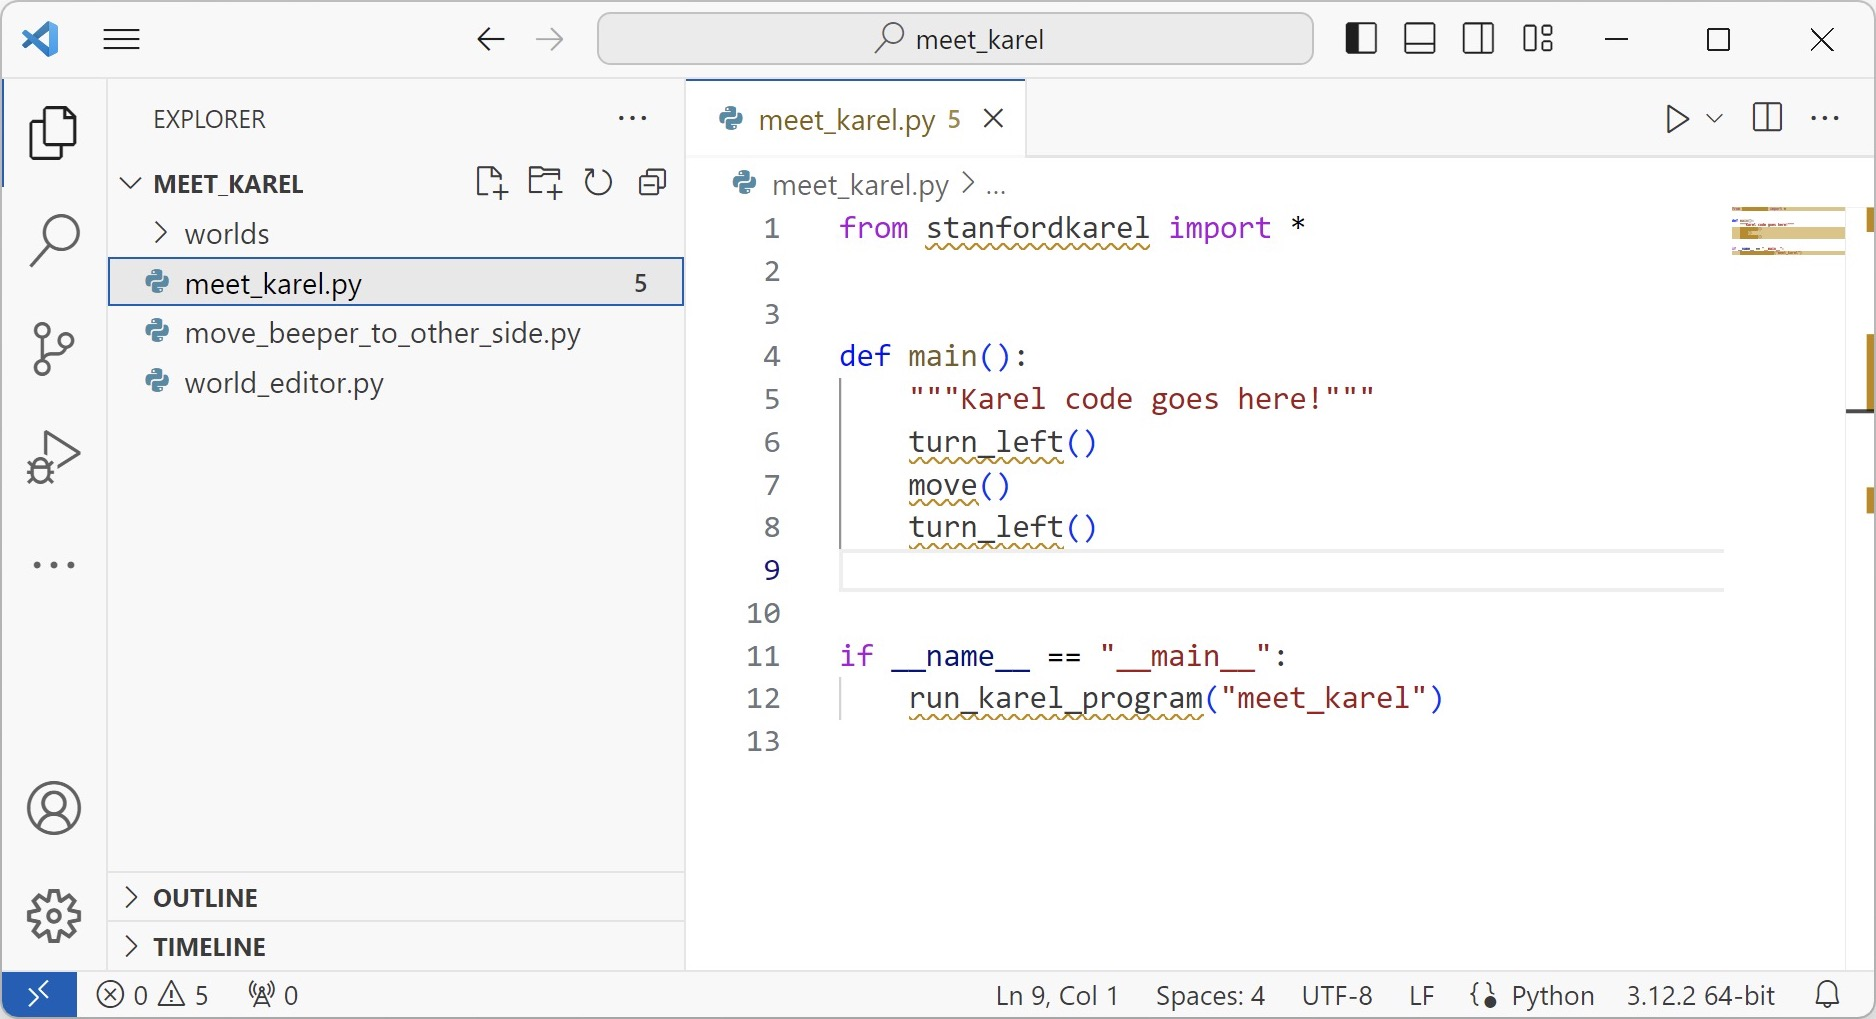
\includegraphics[width=.98\textwidth, trim={2.4mm 2mm 2mm 2mm},clip]{images/vscode_install/v7.jpg}};
    \drawshadow{image}
\end{tikzpicture}
\caption{} 
\label{fig:edtmtkrl}
\end{figure}

\begin{figure}[tbh!]
\begin{tikzpicture}
    \node[anchor=south west,inner sep=0] (image) at (0,0)
        {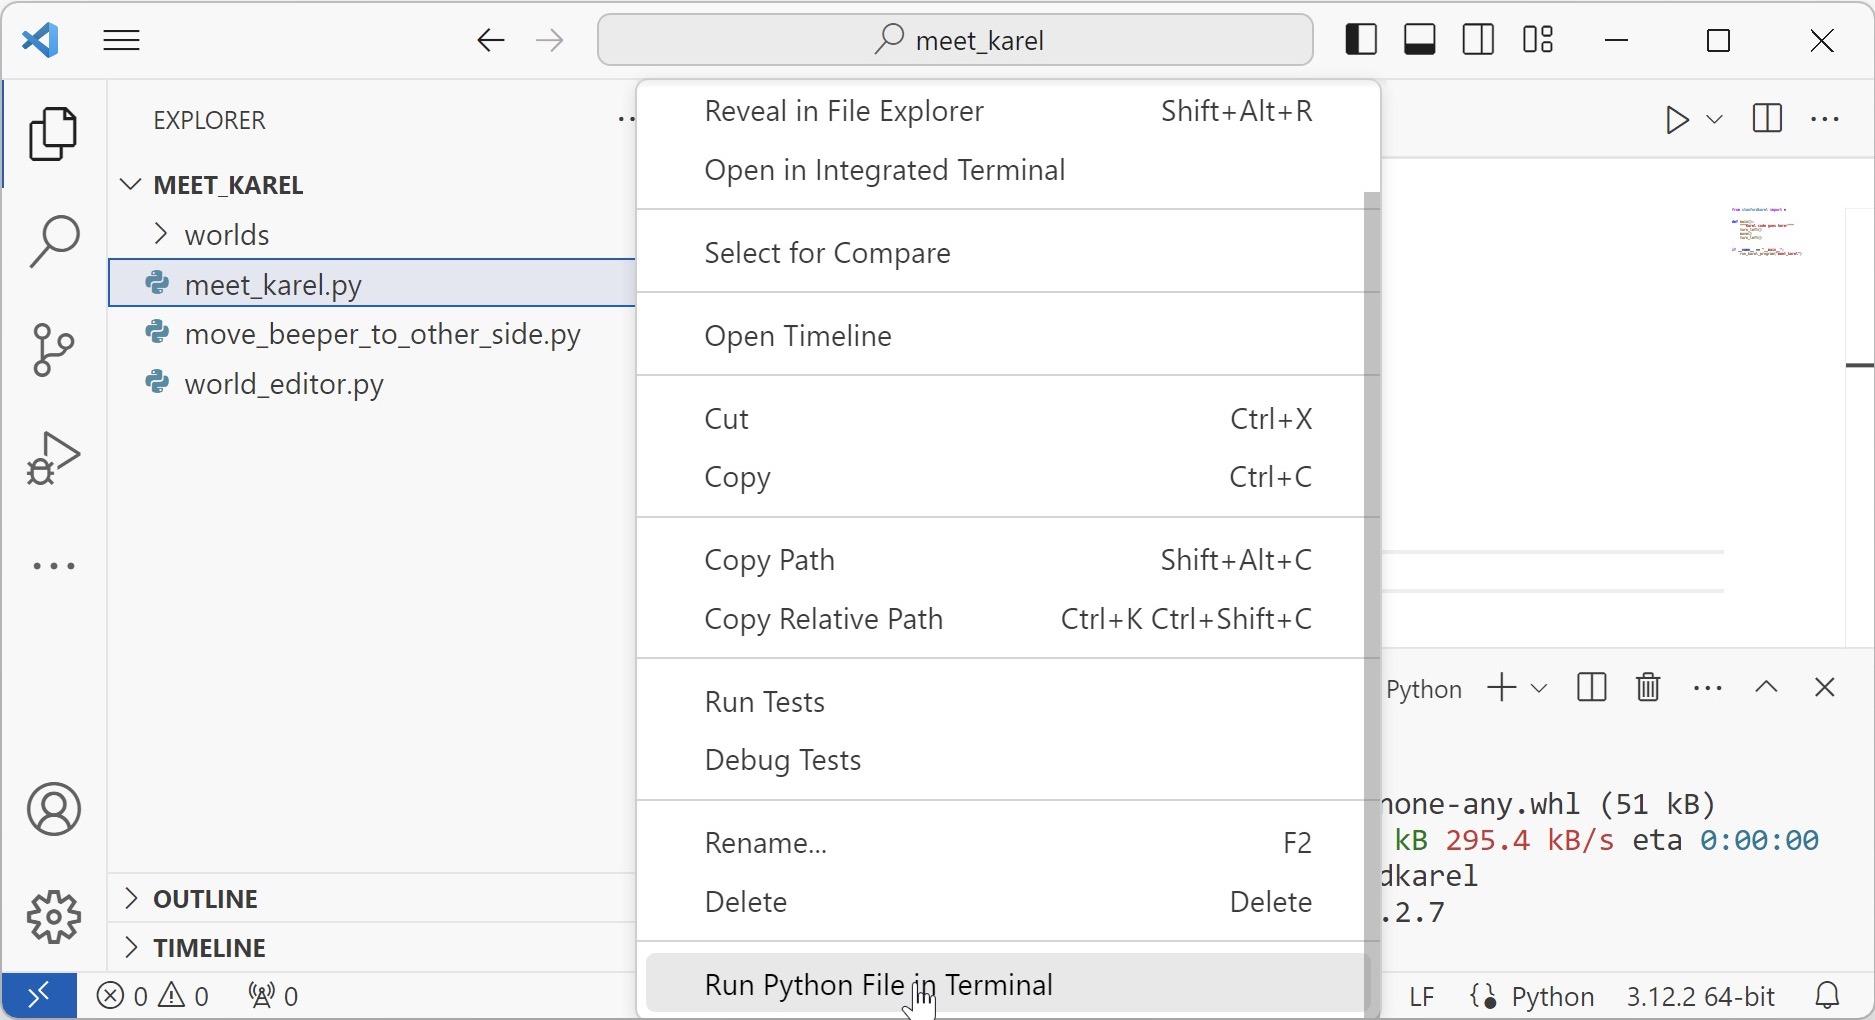
\includegraphics[width=.98\textwidth, trim={2.4mm 2mm 2mm 2mm},clip]{images/vscode_install/v9.jpg}};
    \drawshadow{image}
\end{tikzpicture}
\caption{} 
\label{fig:runmtkrl2}
\end{figure}

\begin{figure}[tbh!]
\begin{tikzpicture}
    \node[anchor=south west,inner sep=0] (image) at (0,0)
        {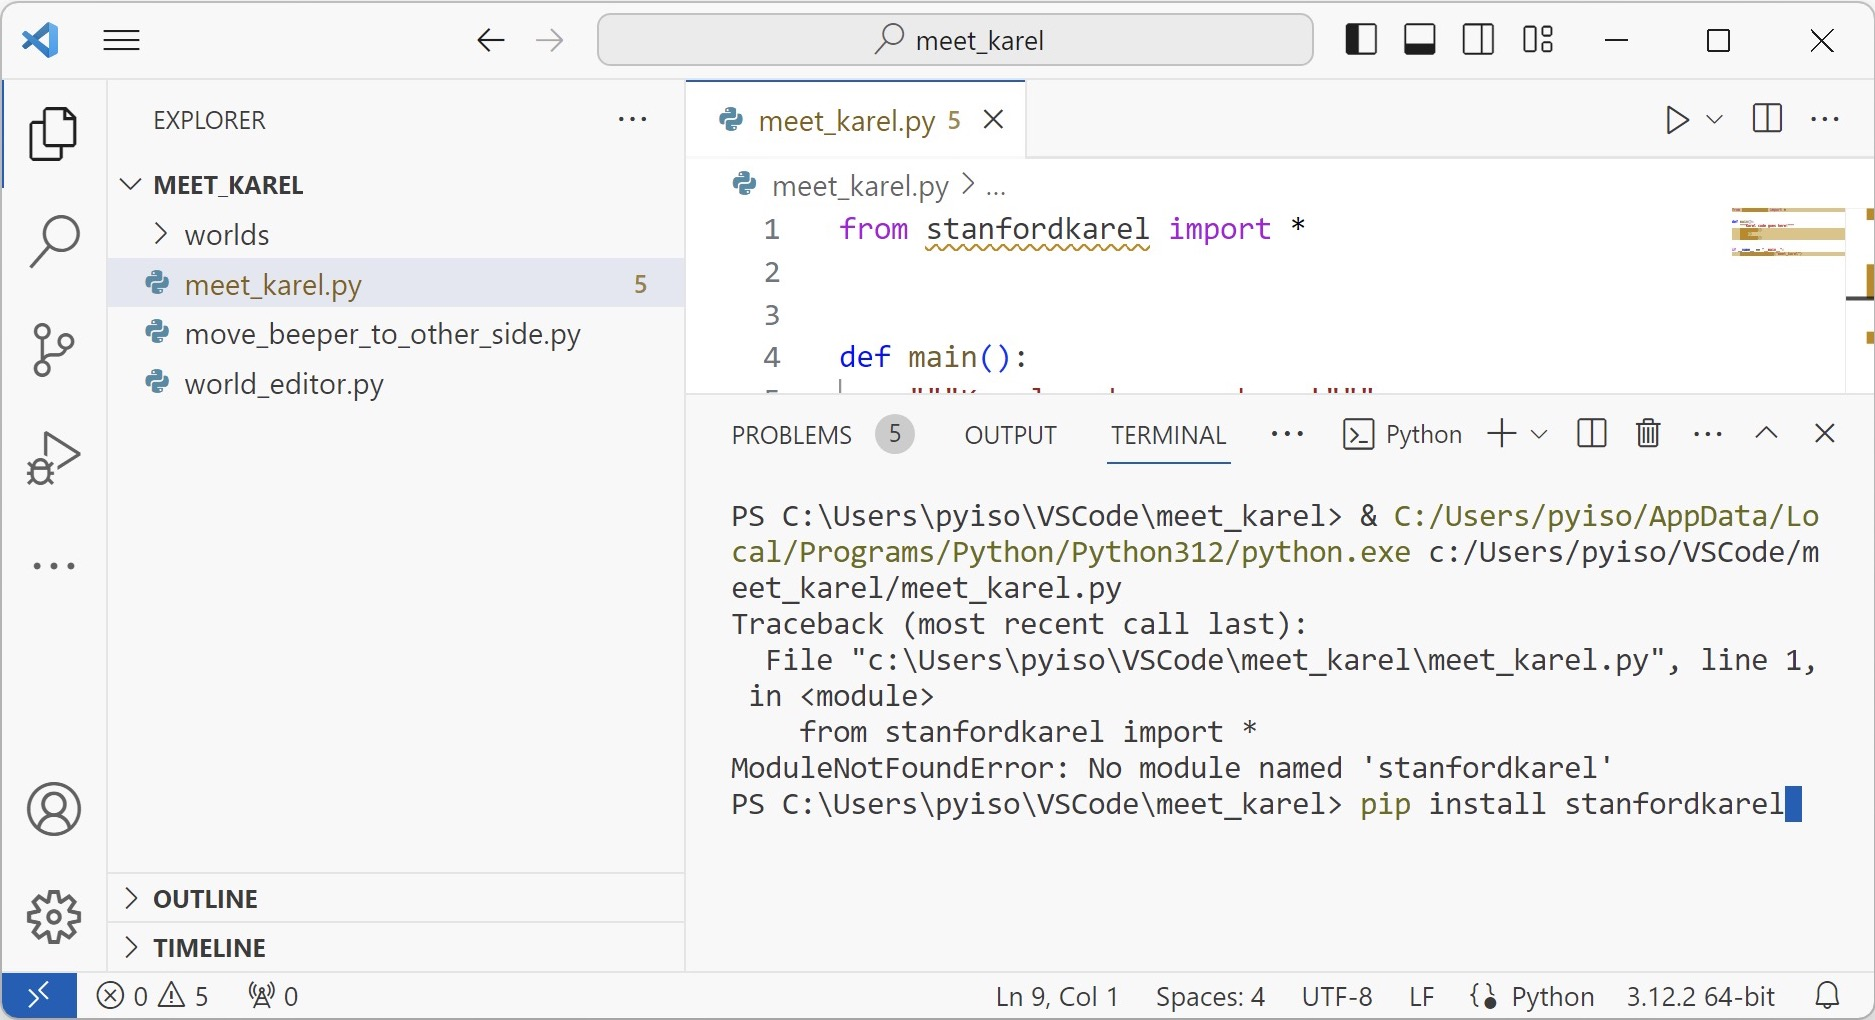
\includegraphics[width=.98\textwidth, trim={2.4mm 2mm 2mm 2mm},clip]{images/vscode_install/v8.jpg}};
    \drawshadow{image}
\end{tikzpicture}
\caption{} 
\label{fig:mtkrlfstrun}
\end{figure}
ခုနကပွင့်လာတဲ့ \fEnSnd{Terminal} မှာပဲ အောက်ပါကွန်မန်းကို \fEn{run} ပြီး \fEnSnd{stanfordkarel} လိုက်ဘရီကို အင်စတောလ်လုပ်ပါ။ 
%
\begin{minted}[frame=lines, framerule=0pt]{text}
pip install stanfordkarel
\end{minted}
%
ပုံ (\fRefNo{\ref{fig:mtkrlfstrun}}) မှာ အနီဝိုင်းထားတာကို ကြည့်ပါ။ အဲဒီအတိုင်းရိုက်ထည့်ပြီး \fEnSnd{Enter} ကီးနှိပ်ပါ။ ခဏကြာတဲ့အခါ အခုလို \fOpn{မက်ဆေ့ချ်}တွေ ကျလာပါလိမ့်မယ်။ 

%
\begin{minted}[frame=lines, framerule=0pt,escapeinside=ßß]{text}
ModuleNotFoundError: No module named 'stanfordkarel'
PS C:\Users\pyiso\VSCode\meet_karel> pip install stanfordkarel
Collecting stanfordkarel
  Downloading stanfordkarel-0.2.7-py3-none-any.whl (51 kB)
     ━━━━━━━━━━━━━━━━━━━━━━━ 51.9/51.9 kB 295.4 kB/s eta 0:00:00
Installing collected packages: stanfordkarel
ß\mytcboxinl[yellow]{Successfully installed stanfordkarel-0.2.7}ß
PS C:\Users\pyiso\VSCode\meet_karel> 
\end{minted}
%
ဟိုက်လိုက်ပြထားတဲ့ \fOpn{မက်ဆေ့ချ်} တွေ့ရရင် အင်စတောလ် အောင်မြင်လို့ပါ။ ပုံ (\fRefNo{\ref{fig:edtmtkrl}}) အယ်ဒီတာမှာလို သတိပေး လှိုင်းတွန့်မျဉ်းတွေ မရှိသင့်တော့ဘူး။ \fEnSnd{stanfordkarel} လိုက်ဘရီ အင်စတောလ် လုပ်ပြီးပြီမိုလို့ သတိပေးတာတွေ ပျောက်သွားသင့်တယ်။


\mytcboxinl{\fEnSnd{meet\_karel.py}} ဖိုင်ကို ညာကလစ်နှိပ်ပြီး \mytcboxinl{\fEnSnd{Run Python File in Terminal}} ပြန်လုပ်ကြည့်ပါ။ ပုံ (\fRefNo{\ref{fig:mtkrlprgm}}) မှာပြထားတဲ့ ကားရဲလ်ပရိုဂရမ် ပွင့်လာသင့်ပါတယ်။ \mytcboxinl{\fEnSnd{Run Program}} နှိပ်ကြည့်ပါ။ စက်ရုပ်လေး ကားရဲလ် နေရာရွေ့သွားတာ တွေ့ရမယ်။ \mytcboxinl{\fEnSnd{meet\_karel.py}} ကို အောက်ပါအတိုင်း ဖြည့်စွက်ရေးပါ။
\begin{figure}[tbh!]
\begin{tikzpicture}
    \node[anchor=south west,inner sep=0] (image) at (0,0)
        {\includegraphics[width=.98\textwidth, trim={2.4mm 2mm 2mm 2mm},clip]{images/vscode_install/mtkrlprgm.jpg}};
    \drawshadow{image}
\end{tikzpicture}
\caption{} 
\label{fig:mtkrlprgm}
\end{figure}


%
\setlength{\fboxsep}{0pt}
\begin{minted}[frame=\mintframe, framerule=\mintrule,framesep= \mintsep, xleftmargin=\xlftmargin
                , bgcolor=mintbgcolor,rulecolor=mintrulecolor
                , python3=true]{python}
from stanfordkarel import *


def main():
    """Karel code goes here!"""
    move()
    move()
    move()
    pick_beeper()
    turn_left()
    move()
    move()

    turn_left()
    turn_left()
    turn_left()

    move()
    put_beeper()


if __name__ == "__main__":
    run_karel_program("meet_karel")
\end{minted}
%

\mytcboxinl{\fEnSnd{meet\_karel.py}} ဖိုင်ကို ညာကလစ်နှိပ်ပြီး \mytcboxinl{\fEnSnd{Run Python File in Terminal}} ပြန်လုပ်ကြည့်ပါ။ ကားရဲလ်ပရိုဂရမ် ပွင့်လာရင် \mytcboxinl{\fEnSnd{Run Program}} နှိပ်ကြည့်ပါ။ ဘိပါလေးကို နေရာရွှေ့ပေးပါလိမ့်မယ်။ အကယ်၍ ကားရဲလ်ပရိုဂရမ် မတက်လာရင် ကုဒ်ရေးတာမှားနေလို့ ဖြစ်နိုင်တယ်။ အပေါ်ကုဒ်နဲ့ နှိုင်းယှဉ်ပြီး ကြည့်ပါ။ \fEn{VS Code} အယ်ဒီတာမှာ အနီလှိုင့်တွန့်လေးတွေ ပြတဲ့နေရင် အဲဒီနေရာတွေမှာ ဆင်းတက်စ်မှားနေတာ ဖြစ်နိုင်တယ်။
%
\begin{mytcbox}
\fEn{VS Code} အယ်ဒီတာမှာ ပရိုဂရမ်ကုဒ်ပြင်ပြီး ပြန် \fEn{run} တဲ့အခါ ပထမ \fEn{run} ထားတဲ့ ပရိုဂရမ်ကို အရင်ပိတ်ဖို့လိုပါတယ်။ ဆိုလိုတာက \fEnSnd{meet\_karel.py} ကို \fEn{run} ထားတယ်ဆိုပါစို့။ ပုံ (\fRefNo{\ref{fig:mtkrlprgm}}) က ဝင်းဒိုးပွင့်လာမယ်။ \fEnSnd{meet\_karel.py} ကုဒ်ကို ပြင်ပြီး ပြန် \fEn{run} ချင်ရင် အဲဒီ ဝင်းဒိုးကို အရင်ပိတ်ရမယ်။ မဟုတ်ရင် ပြင်ထားတဲ့ ပရိုဂရမ်က ချက်ချင်း ပွင့်မလာဘူး။ ပထမ ဟာကို ပိတ်တော့မှပဲ နောက် \fEn{run} တဲ့ဟာ ပွင့်လာမှာ။ 
\end{mytcbox}
%
ဝိုက်ကွင်းကျန်နေတာက အဖြစ်များတဲ့ အမှားပါ။ ကျန်ခဲ့လို မရပါဘူး။ အင်ဒန့်တေးရှင်း \fEn{(indentation)} လုပ်ရမဲ့နေရာမှာ မလုပ်ထားရင်လည်း ပြဿနာဖြစ်တယ်။ \fCode{move}\fEn{,} \fCode{turn\_left} တွေကို ဘေးမျဉ်းညာဘက်ခွာပြီး အင်ဒန့်လုပ်ပေးရမယ်။ အဲဒါတွေ ဂရုမစိုက်မိရင် ဆင်းတက်စ်အမှားဖြစ်ပြီး ပရိုဂရမ် \fEn{run} လို့ မရနိုင်ဘူး။

\fEnSnd{Terminal} မှာ ထုတ်ပေးတဲ့ \fOpn{မက်ဆေ့ချ်}တွေကို ကြည့်ပြီးတော့လည်း ဘာပြဿနာဖြစ်နေလဲ မှန်းဆလို့ရနိုင်တယ်။ ဘာကြောင့်ဖြစ်နိုင်လဲ ဆက်စပ်စဉ်းစားလို့ ရတယ်။ ဥပမာ ဖြစ်တဲ့ပြဿနာအလိုက် အခုလိုတွေ့ရပါမယ်။ 
%
\begin{minted}[frame=lines, framerule=0pt,escapeinside=ßß]{text}
File "c:\Users\pyiso\VS Code\meet_karel\meet_karel.py", ß\mytcboxinl[yellow]{line 6}ß
    move(
          ^
    ß\mytcboxinl[yellow]{SyntaxError: '(' was never closed}ß
\end{minted}
%
%
\begin{minted}[frame=lines, framerule=0pt,escapeinside=ßß]{text}
File "c:\Users\pyiso\VS Code\meet_karel\meet_karel.py", ß\mytcboxinl[yellow]{line 7}ß
    move()
    ß\mytcboxinl[yellow]{IndentationError: unexpected indent}ß 
\end{minted}
%
%
\begin{minted}[frame=lines, framerule=0pt, escapeinside=ßß]{text}
Traceback (most recent call last):
  File "c:\Users\pyiso\VS Code\meet_karel\meet_karel.py", ß\mytcboxinl[yellow]{line 1}ß, 
        in <module>
    from stanfordkarel import *
    ß\mytcboxinl[yellow]{ModuleNotFoundError: No module named 'stanfordkarel'}ß
\end{minted}
%



\clearpage


\subsection*{VS Code တွင် Python ဖိုင် အသစ်ယူခြင်း}
\fEnSnd{MEET\_KAREL} ပင်မ ပရောဂျက်ဖိုဒါပေါ်မှာ ကလစ်နှိပ်ပါ။ ပုံမှာ ပြထားတဲ့ \mytcboxinl{\fEnSnd{New File}} အိုင်ကွန်ကိုနှိပ်ပါ။ ဖိုင်နံမည်ဖြည့်တဲ့ ဘောက်စ်လေး ပေါ်လာမယ်။ \fEn{Python} ဖိုင်တွေက \fEnSnd{.py} အိပ်စ်တန်းရှင်းနဲ့ ဖြစ်ရပါမယ်။ ဒါကြောင့် နံမည် ဖြည့်တဲ့အခါ \fEnSnd{.py} နဲ့ အဆုံးသတ်ပေးရပါမယ် (ဥပမာ \fEnSnd{hello.py})။ ကားရဲလ်ပရိုဂရမ်တစ်ခုကို \fEn{Python} ဖိုင်တစ်ခု ထားပါမယ်။ ပင်မ ပရောဂျက်ဖိုဒါ အောက်မှာပဲ တိုက်ရိုက်ရှိရပါမယ်။ 

နောက်ပိုင်း အဆင့်မြင့်လာရင် ပရိုဂရမ်တစ်ခုအတွက် ပရောဂျက်တစ်ခု ထားနိုင်တယ်။ ကုဒ်ဖိုင်တွေအပြင် ပရိုဂရမ်အတွက် လိုအပ်တဲ့ ရုပ်ပုံတွေ၊ အခြားဖိုင်တွေ (\fEn{config} ဖိုင်၊ \fEn{setting} ဖိုင် စသည်ဖြင့်) လည်း ပါနိုင်တယ်။ ပင်မပရောဂျက် အောက်မှာပဲ  ဖိုင်တွေက တိုက်ရိုက်ရှိဖို့လည်း မလိုတော့ဘူး။  ဆက်{\allowbreak}စပ်ရာ ဖိုင်တွေကို အမျိုးအစားအလိုက်၊  ဖန်ရှင်အလိုက် ဖိုဒါတွေခွဲပြီး  စနစ်ကျ စီစဉ်ဖွဲ့စည်း ထားရမှာပါ။ ပရောဂျက်တစ်ခုမှာ ဖိုင်တွေကို စနစ်တကျ စုဖွဲ့ထားဖို့ အရေးကြီးပါတယ်။

\begin{figure}[tbh!]
\begin{tikzpicture}
    \node[anchor=south west,inner sep=0] (image) at (0,0)
        {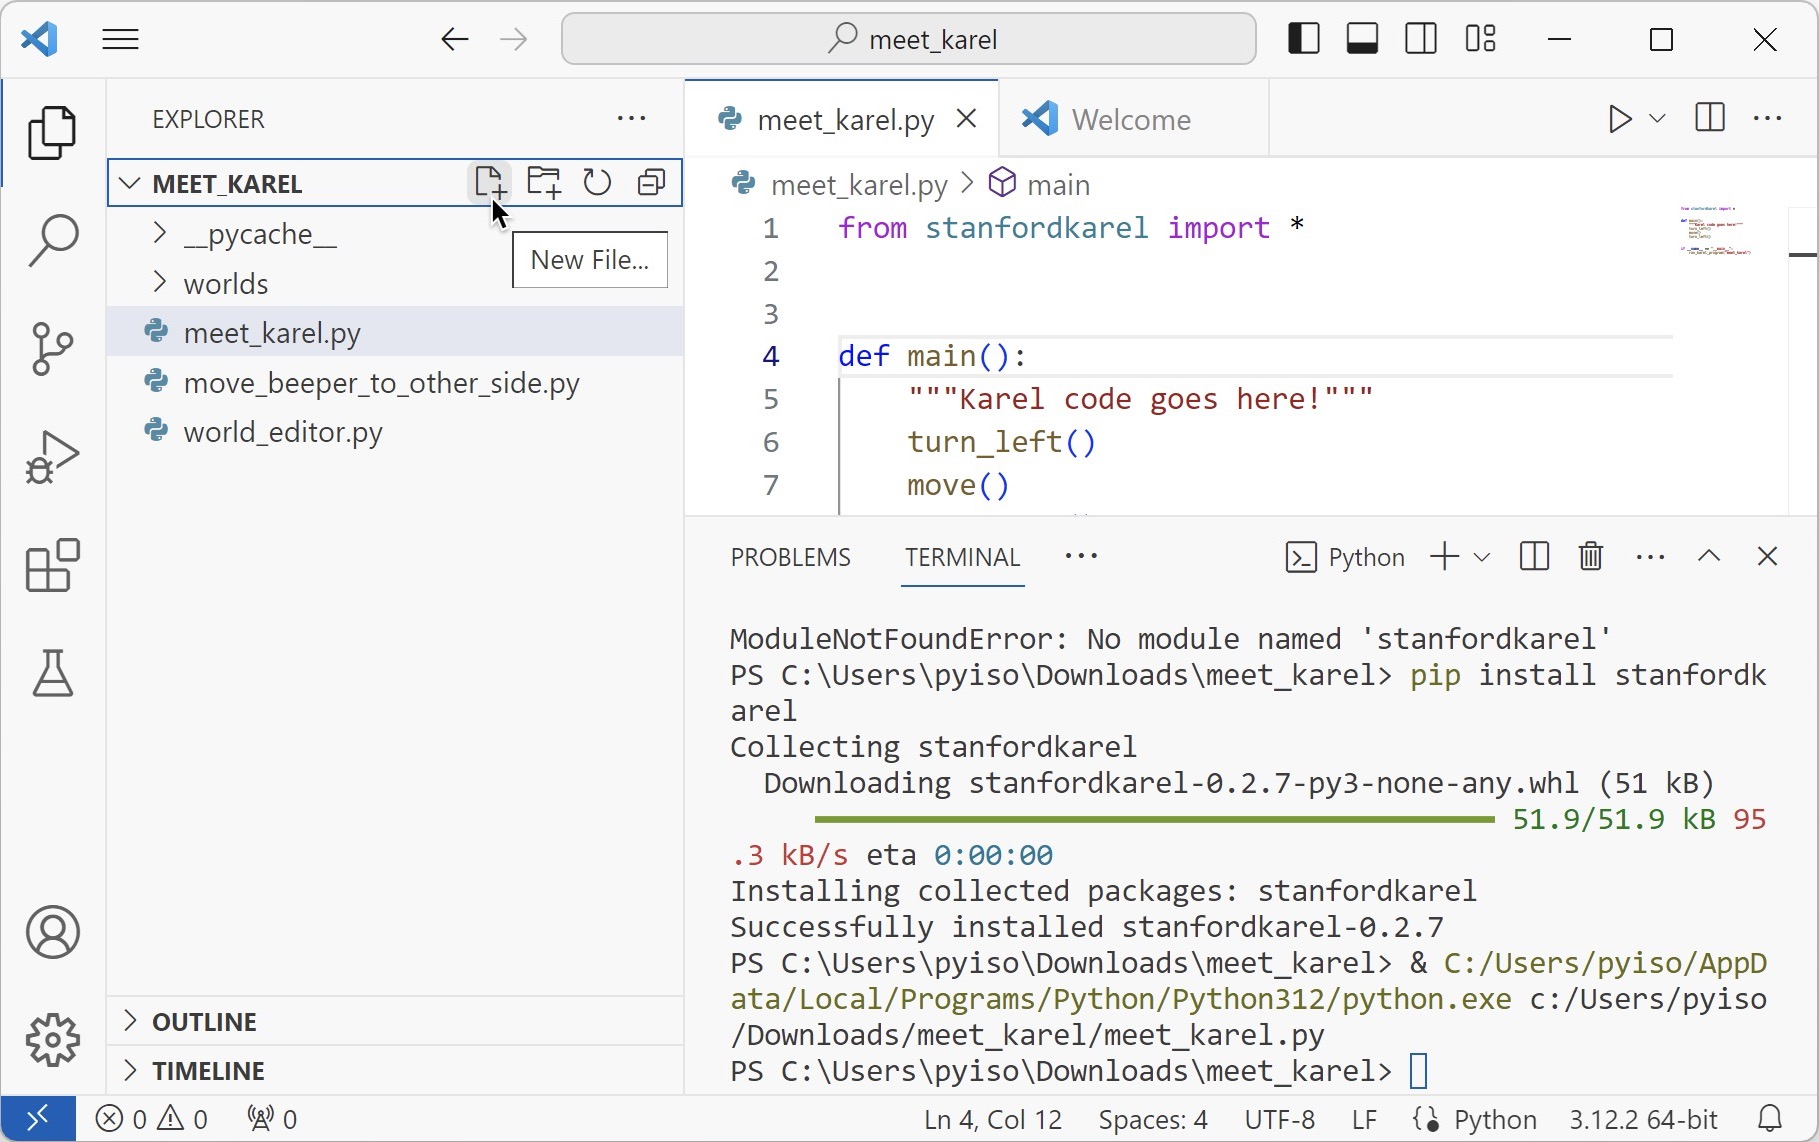
\includegraphics[width=.98\textwidth, trim={2.4mm 2mm 2mm 2mm},clip]{images/vscode_install/newfile.jpg}};
    \drawshadow{image}
\end{tikzpicture}
\caption{} 
\label{fig:vsnewfile}
\end{figure}

\clearpage








\afterpage{\blankpage}

\renewcommand\thefigure{B/\arabic{figure}} 
\chapter{ကားရဲလ်ပရိုဂရမ် ဖီချာများ}\label{apdx:02}

\section*{ကားရဲလ် ကမ္ဘာဖိုင်များ}

ကားရဲလ်ပရိုဂရမ် ဝင်းဒိုးမှာ \mytcboxinl{\fEnSnd{Load World}} ခလုတ်နှိပ်ပြီး ကမ္ဘာဖိုင်အသစ် တင်လို့ရတယ်။ ခလုတ်နှိပ်လိုက်ရင် အခုလို ဖိုင် ဒိုင်ယာလော့ဂ် ပွင့်လာမယ်။

\begin{figure}[tbh!]
\begin{tikzpicture}
    \node[anchor=south west,inner sep=0] (image) at (0,0)
        {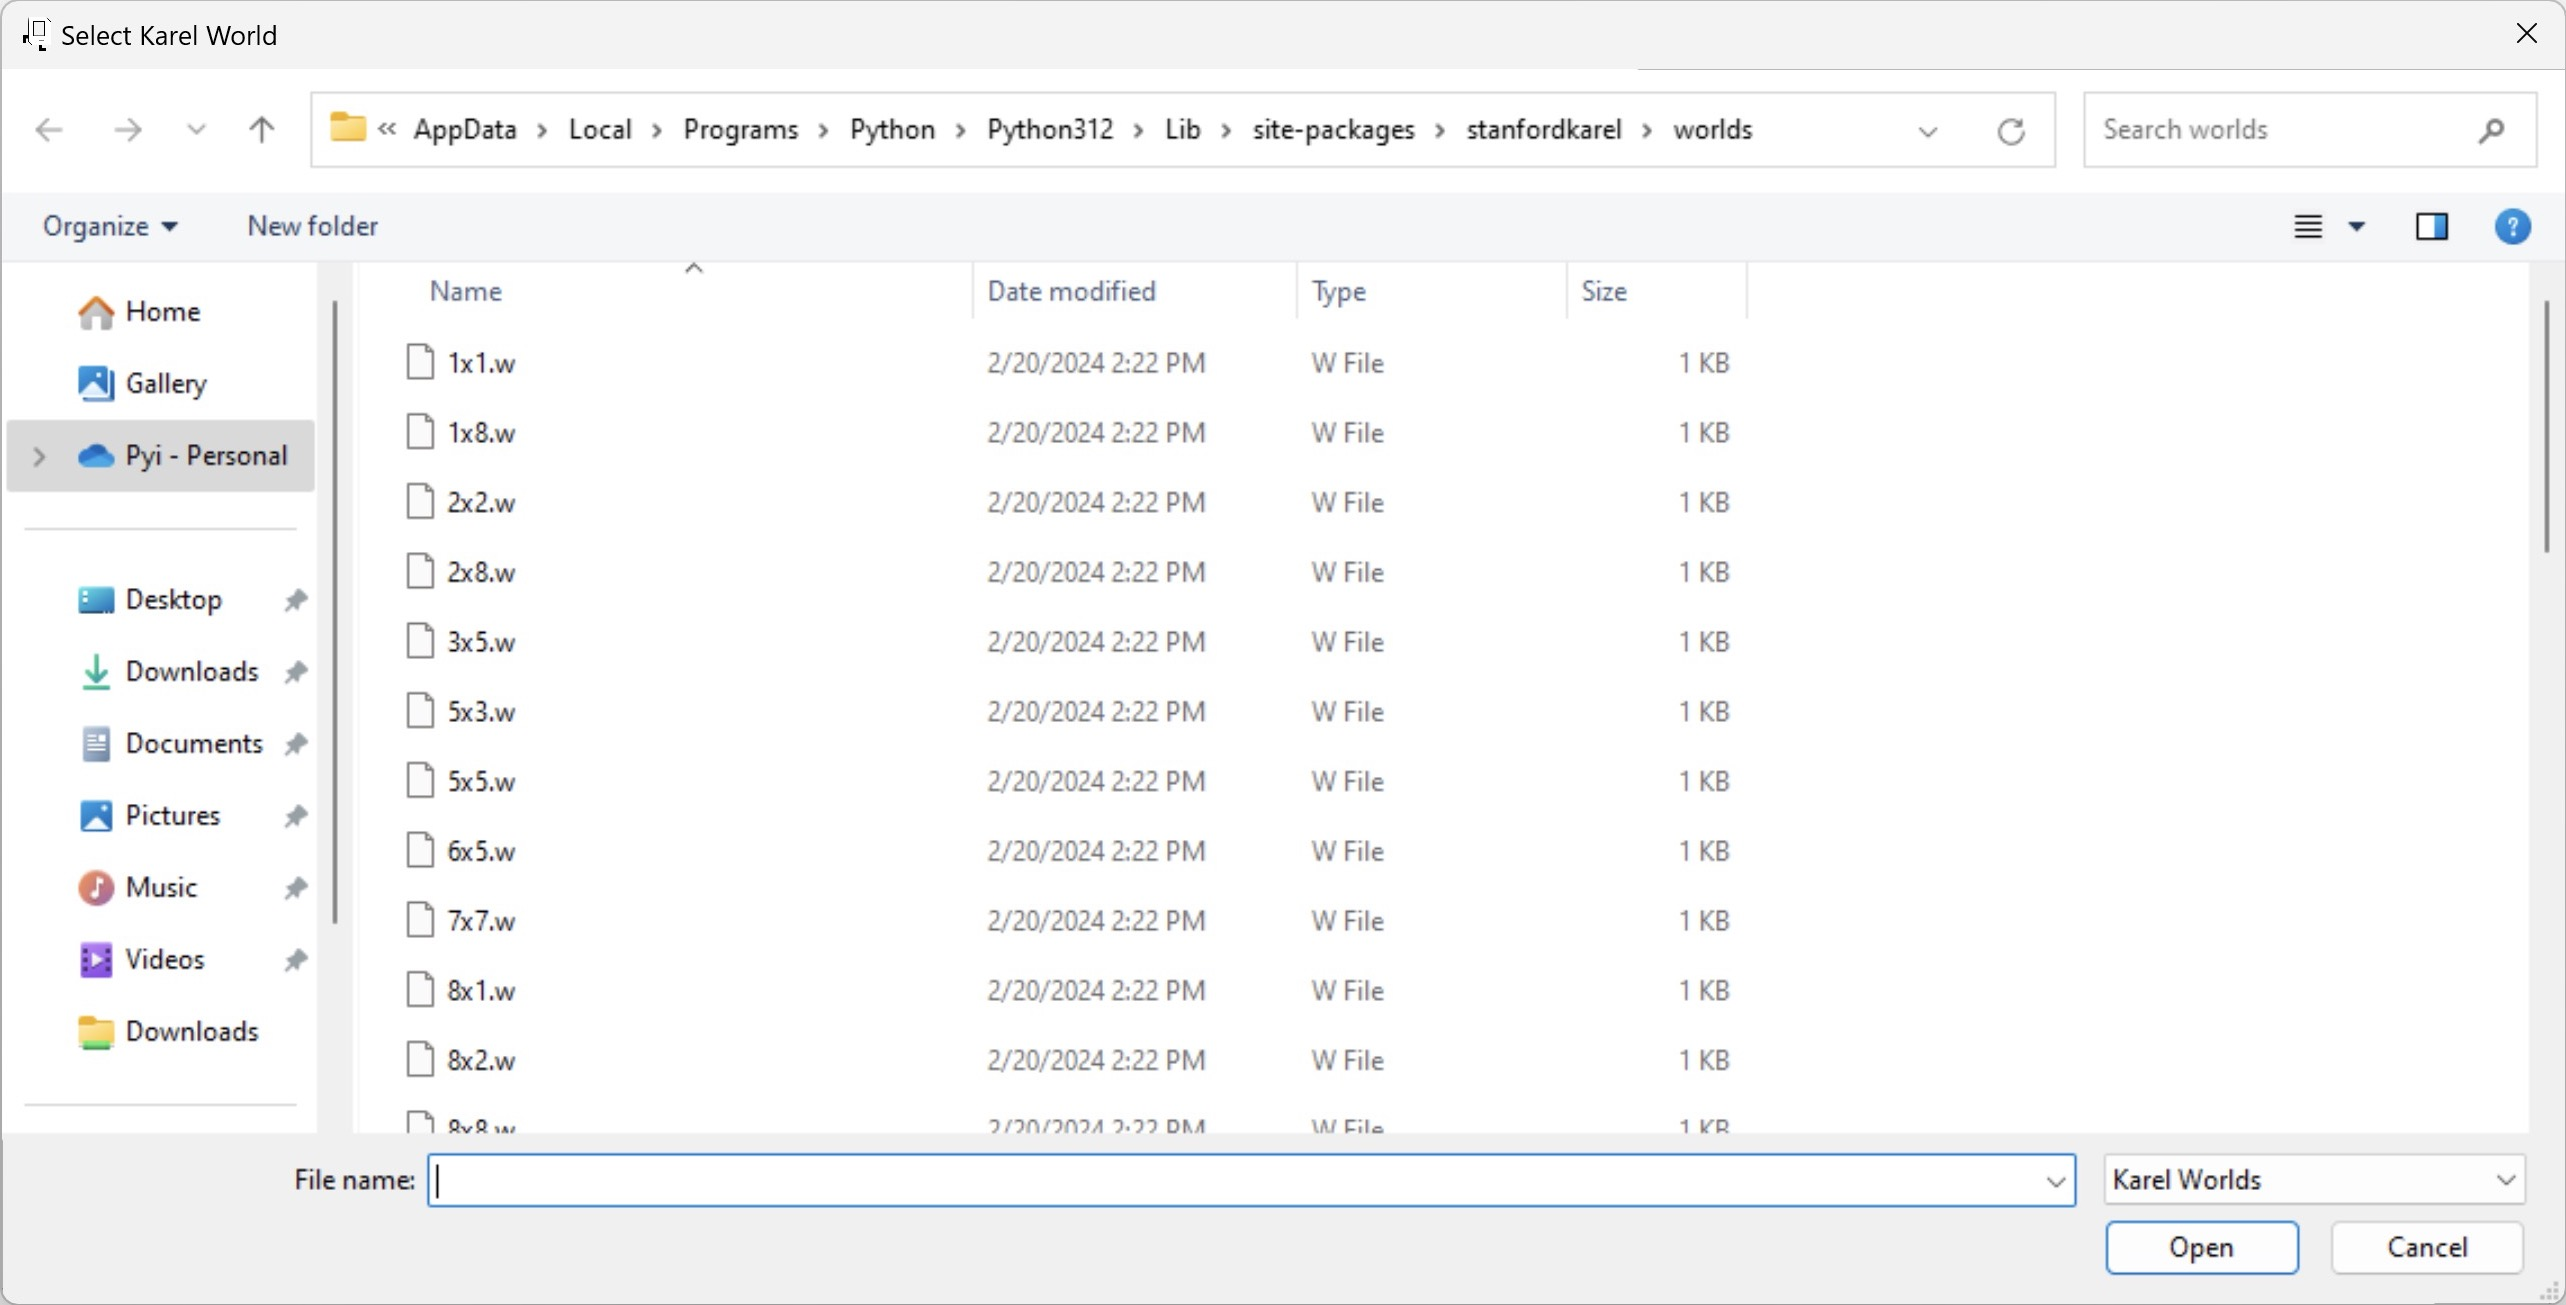
\includegraphics[width=.98\textwidth, trim={2mm 2mm 28cm 2.5mm},clip]{images/apdx02/dftworlds.jpg}};
    \drawshadow{image}
\end{tikzpicture}
\caption{} 
\label{fig:dftworlds}
\end{figure}

ဒါက \fEnSnd{stanfordkarel} လိုက်ဘရီ သူ့နဂိုအရှိအတိုင်း ပါတဲ့ \fEnSnd{worlds} ဖိုဒါပါ။ ဖိုင်တွေက  \mytcboxinl{\fEnSnd{.w}} နဲ့ ဆုံးပါတယ်။  ကမ္ဘာဖိုင်တွေကို ပင်မ ပရောဂျက်အောက် \fEnSnd{worlds} ဖိုဒါထဲမှာ ထားလို့လည်းရတယ်။ အခြားနေရာတွေမှာ ထားလို့တော့ မရဘူး။

စာအုပ်ပါ ဥပမာတွေ၊ လေ့ကျင့်ခန်းတွေအတွက် ကမ္ဘာဖိုင်တွေကို ပရောဂျက် တစ်ခုချင်းအလိုက် သီးခြား \fEnSnd{worlds} ဖိုဒါထဲမှာ ထည့်ပေးထားမှာပါ။ ပရိုဂရမ်တစ်ခုဟာ ကမ္ဘာတစ်ခုတည်းမှာပဲ အလုပ်လုပ်တာမဟုတ်ဘဲ အလားတူ ကမ္ဘာအမျိုးမျိုးအတွက် အလုပ်လုပ်အောင် ရေးပေးရတာ။ အခုပြောတာကို နားမလည်ရင် အခန်း (\fRefNo{\ref{ch:ch02}}) ဖတ်ပြီးရင် နားလည်သွားမှာပါ။

\mytcboxinl{\fEnSnd{Load World}} လုပ်တဲ့အခါ ပွင့်လာတဲ့ ဖိုင် ဒိုင်ယာလော့ဂ်က ကိုယ်လိုချင်တဲ့ \fEnSnd{worlds} ဖိုဒါ မဖြစ်နေဘူး။ သူ့နဂိုပါတဲ့ \fEnSnd{worlds} ဖိုဒါ ဖြစ်နေတယ်။ ကိုယ်ခေါ်တင်ချင်တဲ့ ဖိုင်တွေရှိတဲ့ လက်ရှိပရောဂျက်ရဲ့ \fEnSnd{worlds} ဖိုဒါကို သွားရမယ်။ ဥပမာ \fEn{PyCharm/VS Code} အတွက် \fEnSnd{MeetKarel/meet\_karel} ပရောဂျက် \fEnSnd{worlds} ဖိုဒါ လမ်းကြောင်း အပြည့်အစုံက
%
\begin{minted}[frame=lines, framerule=0pt,escapeinside=ßß]{text}
ß\fEnSnd{C:{\textbackslash}Users{\textbackslash}\textit{yourname}{\textbackslash}VSCode{\textbackslash}meet\_karel{\textbackslash}worlds}ß
ß\fEnSnd{C:{\textbackslash}Users{\textbackslash}\textit{yourname}{\textbackslash}PycharmProjects{\textbackslash}MeetKarel{\textbackslash}worlds}ß
\end{minted}
%
ဖြစ်ပါမယ်။ ဖိုင်ဒိုင်ယာလေ့ဂ်ကနေ ဖော်ပြပါ လက်ရှိပရောဂျက် \fEnSnd{worlds} ဖိုဒါကို တစ်ဆင့်ချင်း သွားပြီး တင်ချင်တဲ့ ကမ္ဘာဖိုင် (\fEnSnd{.w} ဖိုင်) ကို ရွေးရမှာပါ။

အပေါ်ကနည်းနဲ့ အဆင်မပြေခဲ့ရင် အခုလိုစမ်းကြည့်ပါ။ လက်ရှိပရောဂျက် \fEnSnd{worlds} ဖိုဒါကို ညာကလစ်နှိပ်ပြီး \fEnSnd{Copy Path} လုပ်ပါ (ပုံ \fRefNo{\ref{fig:cpwldfld}}) ။ ဖိုင် ဒိုင်ယာလော့ဂ် \mytcboxinl{\fEnSnd{File name}} မှာ ကူးထည့်ပါ (ပုံ \fRefNo{\ref{fig:pstepth}})။ \mytcboxinl{\fEnSnd{Enter}} ကီးနှိပ်ပါ။ ပရောဂျက် \fEnSnd{worlds} ဖိုဒါကိုရောက်သွားပါမယ်။ လိုတဲ့ကမ္ဘာဖိုင် ရွေးတင်ရုံပါပဲ။ ပုံ (\fRefNo{\ref{fig:prjwlds}}) မှာ \fEnSnd{meet\_karel} \fEnSnd{worlds} ကို နမူနာပြထားပါတယ်။

\begin{figure}[tbh!]
\begin{tikzpicture}
    \node[anchor=south west,inner sep=0] (image) at (0,0)
        {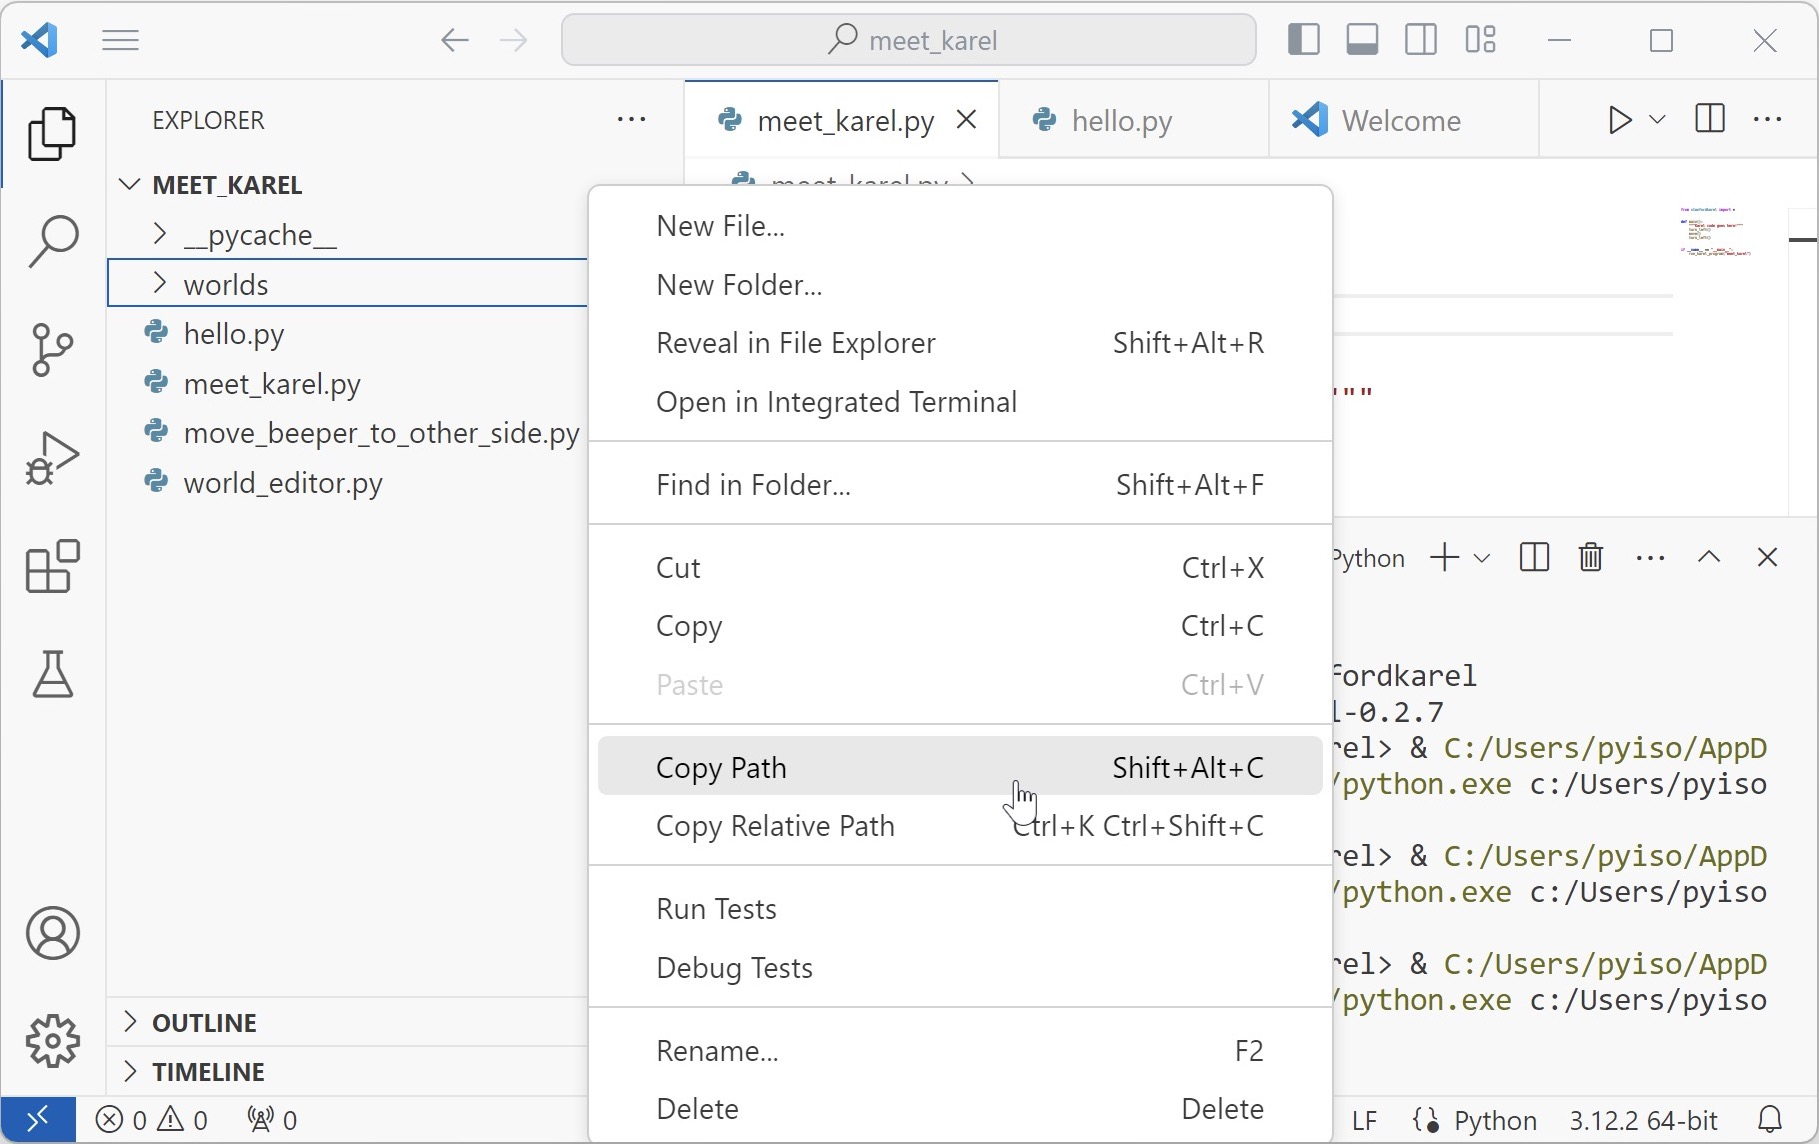
\includegraphics[width=.98\textwidth, trim={2.4mm 2mm 2mm 2mm},clip]{images/apdx02/cpwldfld.jpg}};
    \drawshadow{image}
\end{tikzpicture}
\caption{} 
\label{fig:cpwldfld}
\end{figure}

\begin{mytcbox}
အကယ်၍ အထက်ဖော်ပြပါနည်းတွေက ရှုပ်နေတယ်ထင်ရင်  မှတ်ရ/သွားရ လွယ်တဲ့ \fEnSnd{Desktop, Downloads, Documents} လို နေရာတစ်ခုခုမှာ  သီးသန့်ဖိုဒါတစ်ခု ဆောက်ပြီး ပရောဂျက်အားလုံး ထည့်ထားတာ အရှင်းဆုံးပါပဲ။ ပရောဂျက်ဖိုဒါနေရာ သိရင် ဖိုင်ဒိုင်ယာလော့ဂ်ကနေ ဘယ်လိုမဆို ရောက်အောင် သွားလို့ရပါတယ်။
\end{mytcbox}

\begin{figure}[tbh!]
\begin{tikzpicture}
    \node[anchor=south west,inner sep=0] (image) at (0,0)
        {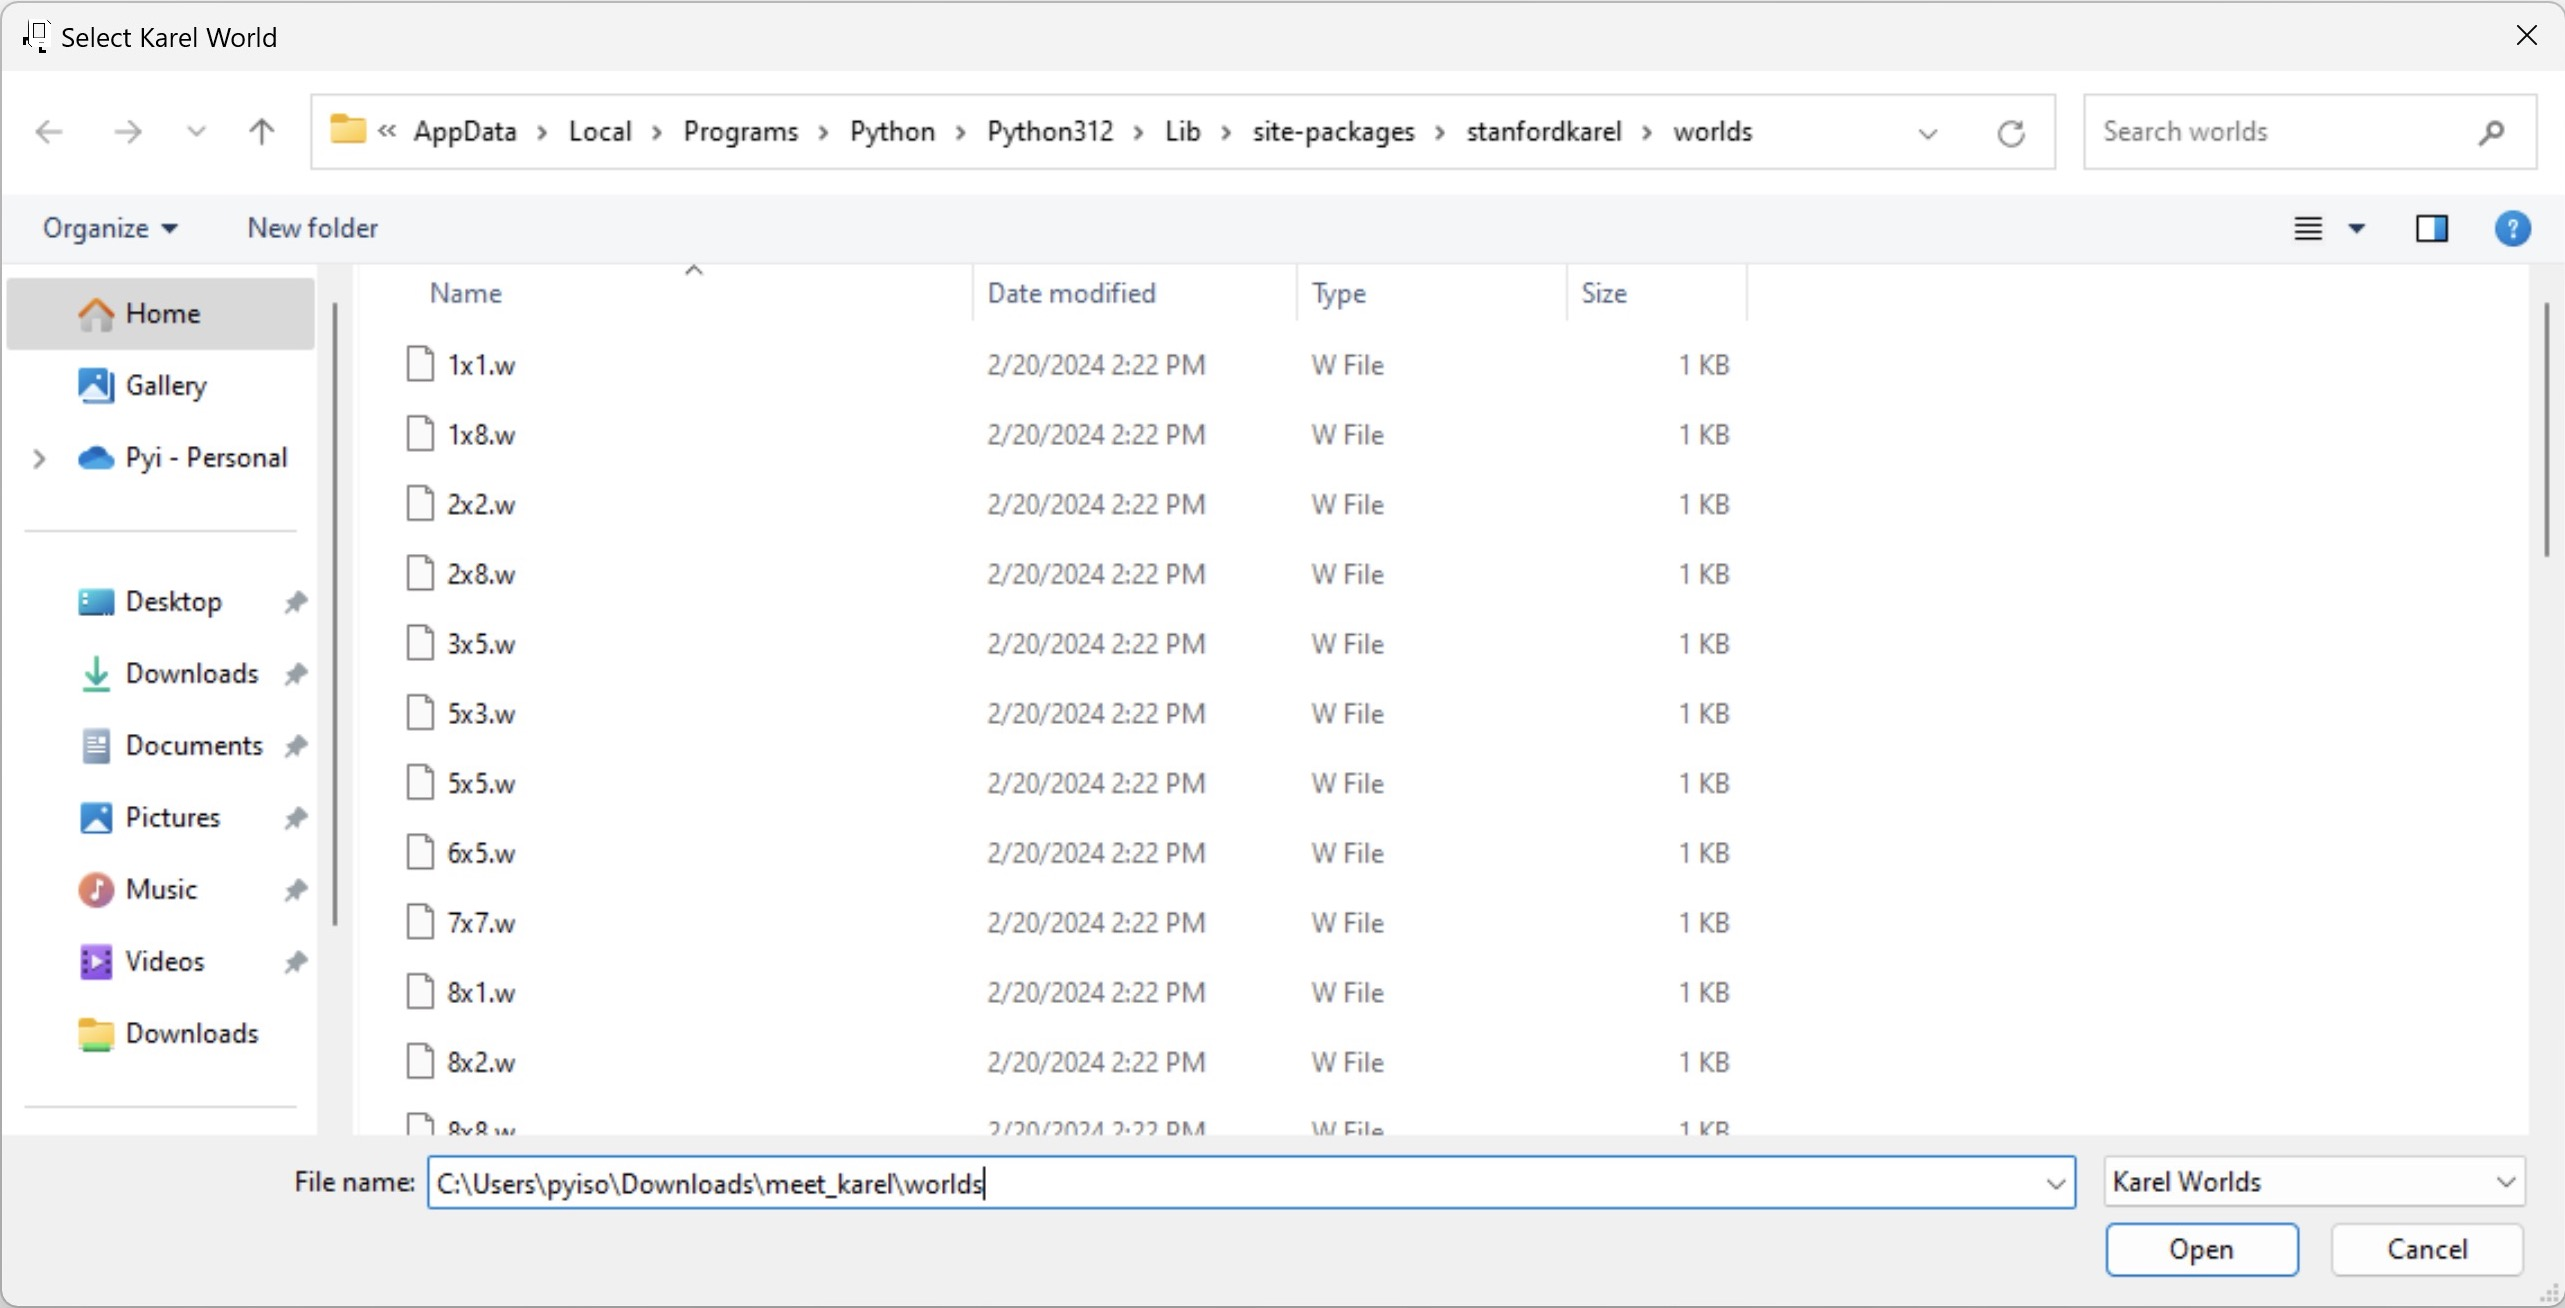
\includegraphics[width=.98\textwidth, trim={2.4mm 2mm 28cm 2mm},clip]{images/apdx02/pstepth.jpg}};
    \drawshadow{image}
\end{tikzpicture}
\caption{} 
\label{fig:pstepth}
\end{figure}

\begin{figure}[tbh!]
\begin{tikzpicture}
    \node[anchor=south west,inner sep=0] (image) at (0,0)
        {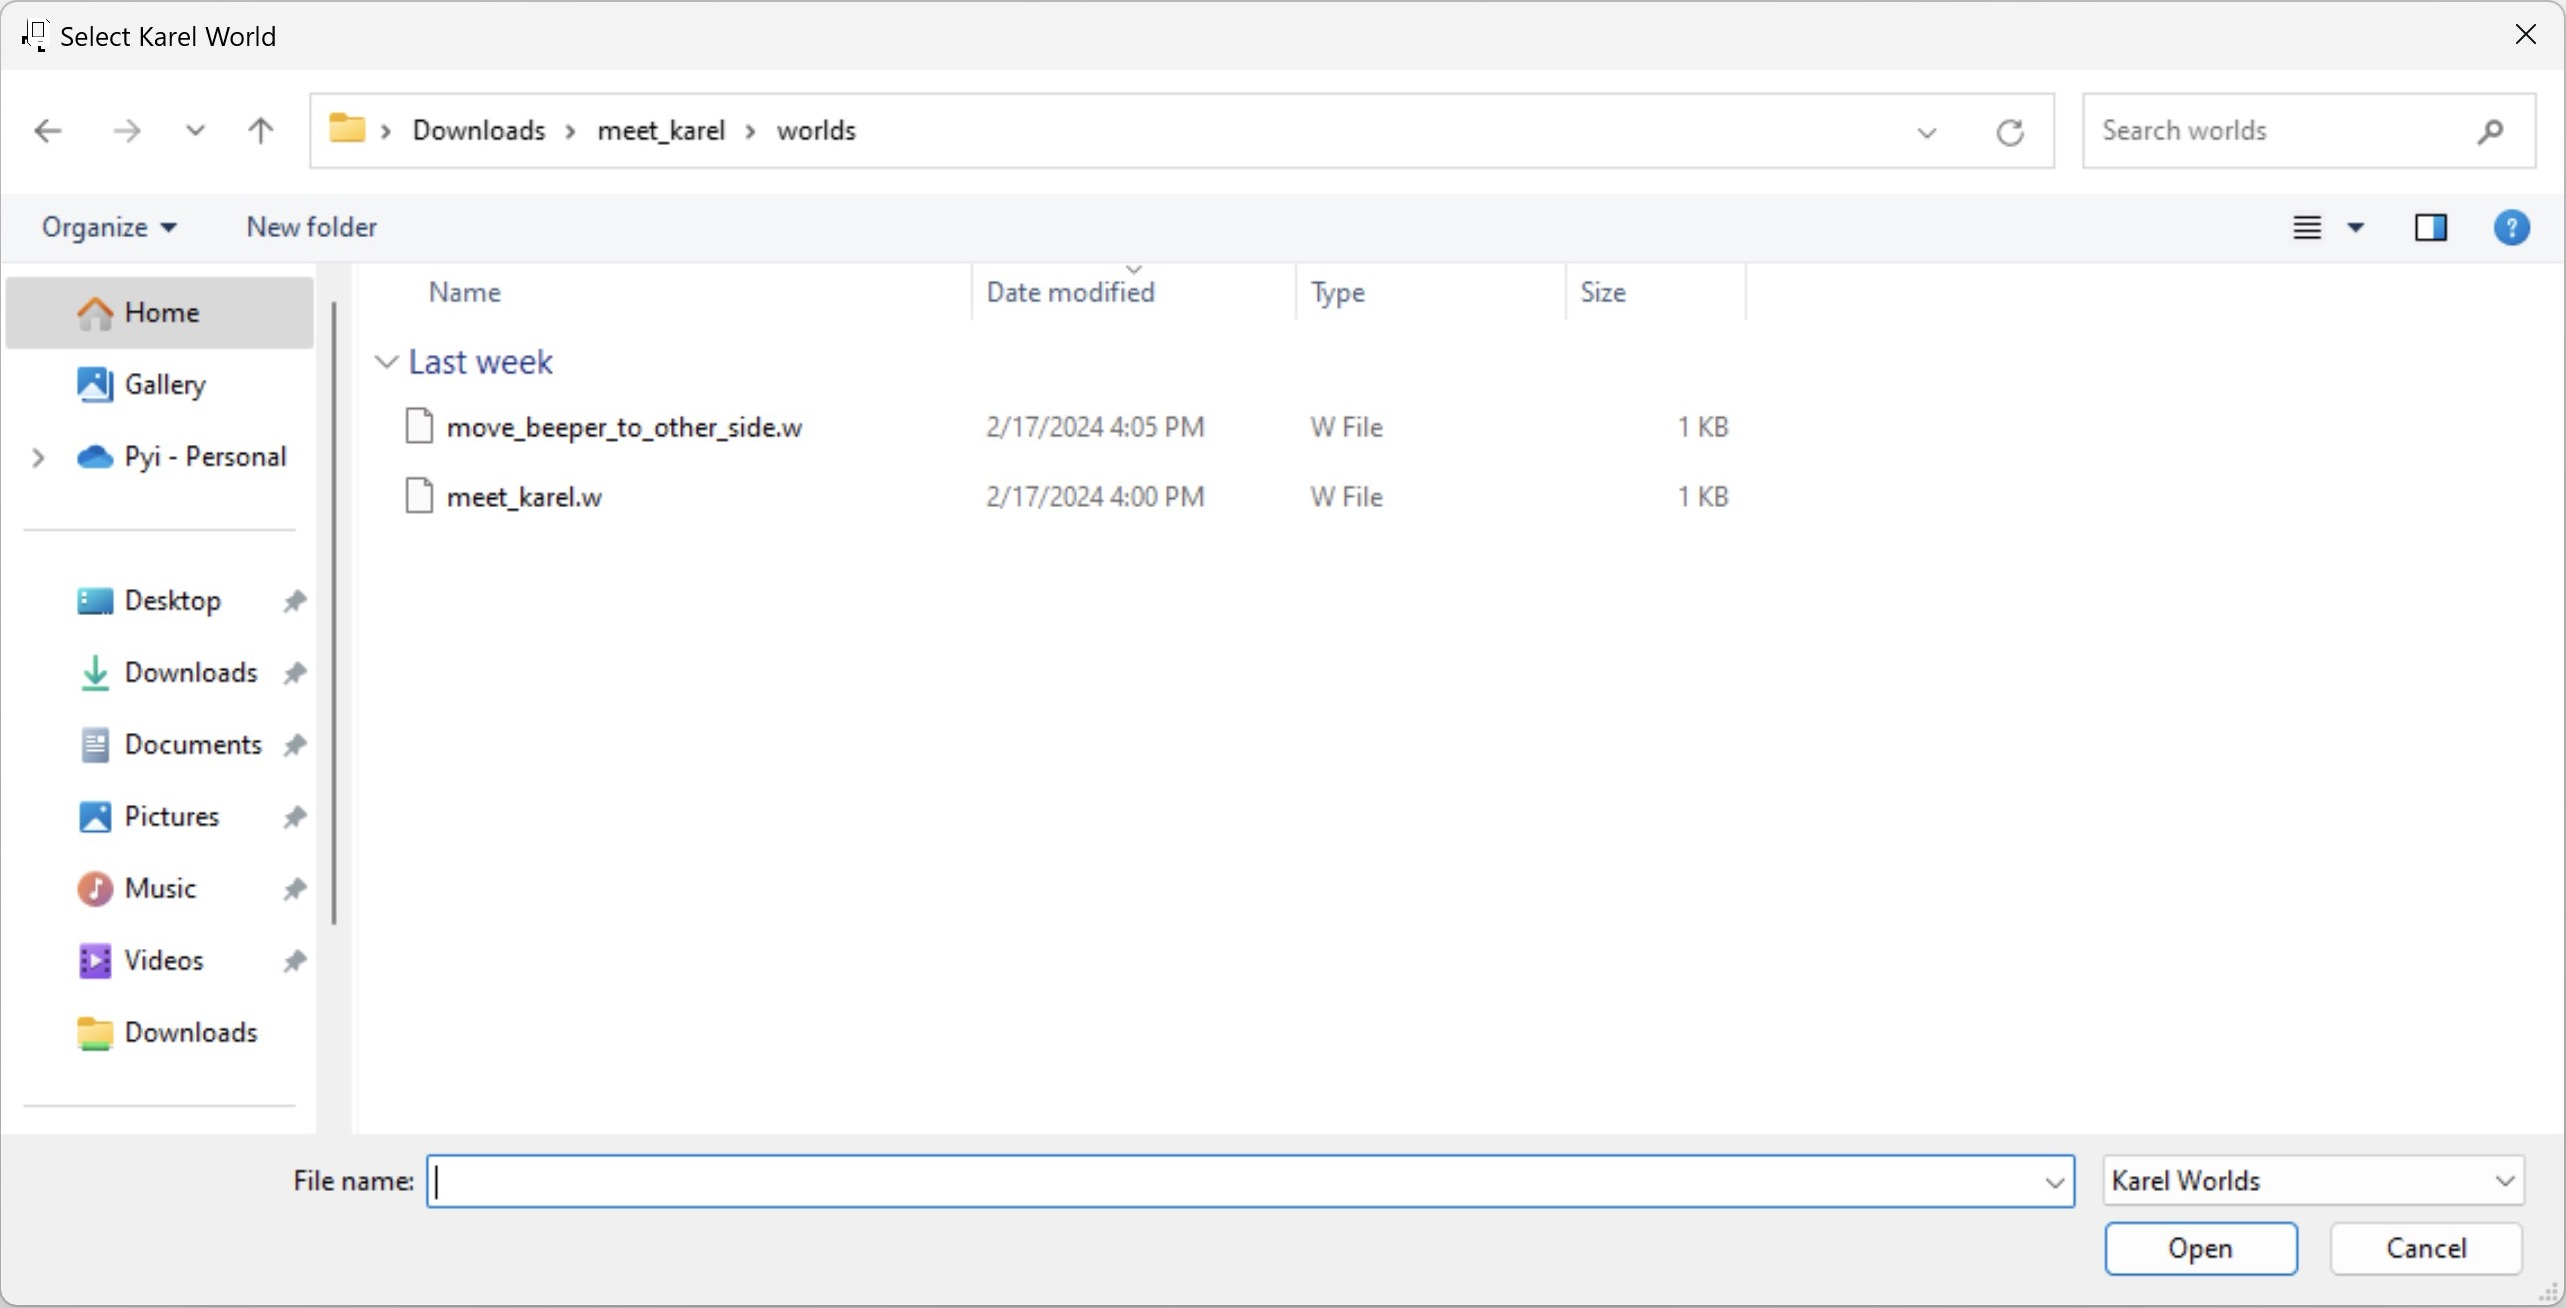
\includegraphics[width=.98\textwidth, trim={2.4mm 2mm 28cm 2mm},clip]{images/apdx02/prjwlds.jpg}};
    \drawshadow{image}
\end{tikzpicture}
\caption{} 
\label{fig:prjwlds}
\end{figure}


\clearpage

\section*{ကိုယ်ပိုင် ကားရဲလ်ကမ္ဘာ ဆောက်ခြင်း }
ကားရဲလ်ရဲ့ ကမ္ဘာ အသစ်တစ်ခုဆောက်မယ်ဆိုရင် \fEnSnd{world\_editor.py} ဖိုင်ကို ညာကလစ်နှိပ်  \fEnSnd{\mytcboxinl{Run}} ပါ။ \mytcboxinl{\fEnSnd{Would you like to load an existing world?}} လို့ ပေါ်လာပြီး \fEnSnd{Yes/No} ရွေးခိုင်ပါလိမ့်မယ်။ \fEnSnd{No} ကို နှိပ်ပါ။ ကမ္ဘာအရွယ်အစားအတွက် ကော်လံ ဘယ်နှစ်ခုလဲ၊ \fEn{row} ဘယ်နှစ်ခုလဲ ထည့်ပေးပါ။  ကိုယ်ပိုင် ကားရဲလ်ကမ္ဘာ တည်ဆောက်လို့ရတဲ့ ဝင်းဒိုးပွင့်လာပါလိမ့်မယ်။ ကားရဲလ် မျက်နှာမူရာအရပ်၊ ဘိပါအိတ်ထဲရှိ ဘိပါအရေအတွက်၊ နံရံဆောက်/ဖျက်တာ၊ ဘိပါထည့်/ဖယ်ထုတ်တာ စတာတွေ လုပ်နိုင်ပါတယ်။  \mytcboxinl{\fEnSnd{Save World}} နှိပ်ပြီး သိမ်းနိုင်ပါတယ်။ ဖိုင်ကိုသိမ်းတဲ့အခါ သူ့နဂို သိမ်းခိုင်းတဲ့ဖိုဒါ \fEn{(default world folder)} ထဲမှာ သို့မဟုတ် ပင်မ ပရောဂျက်ဖိုဒါထဲက \fEnSnd{worlds} ဖိုဒါထဲမှာ သိမ်းရပါမယ်။  

\begin{figure}[tbh!]
\begin{tikzpicture}
    \node[anchor=south west,inner sep=0] (image) at (0,0)
        {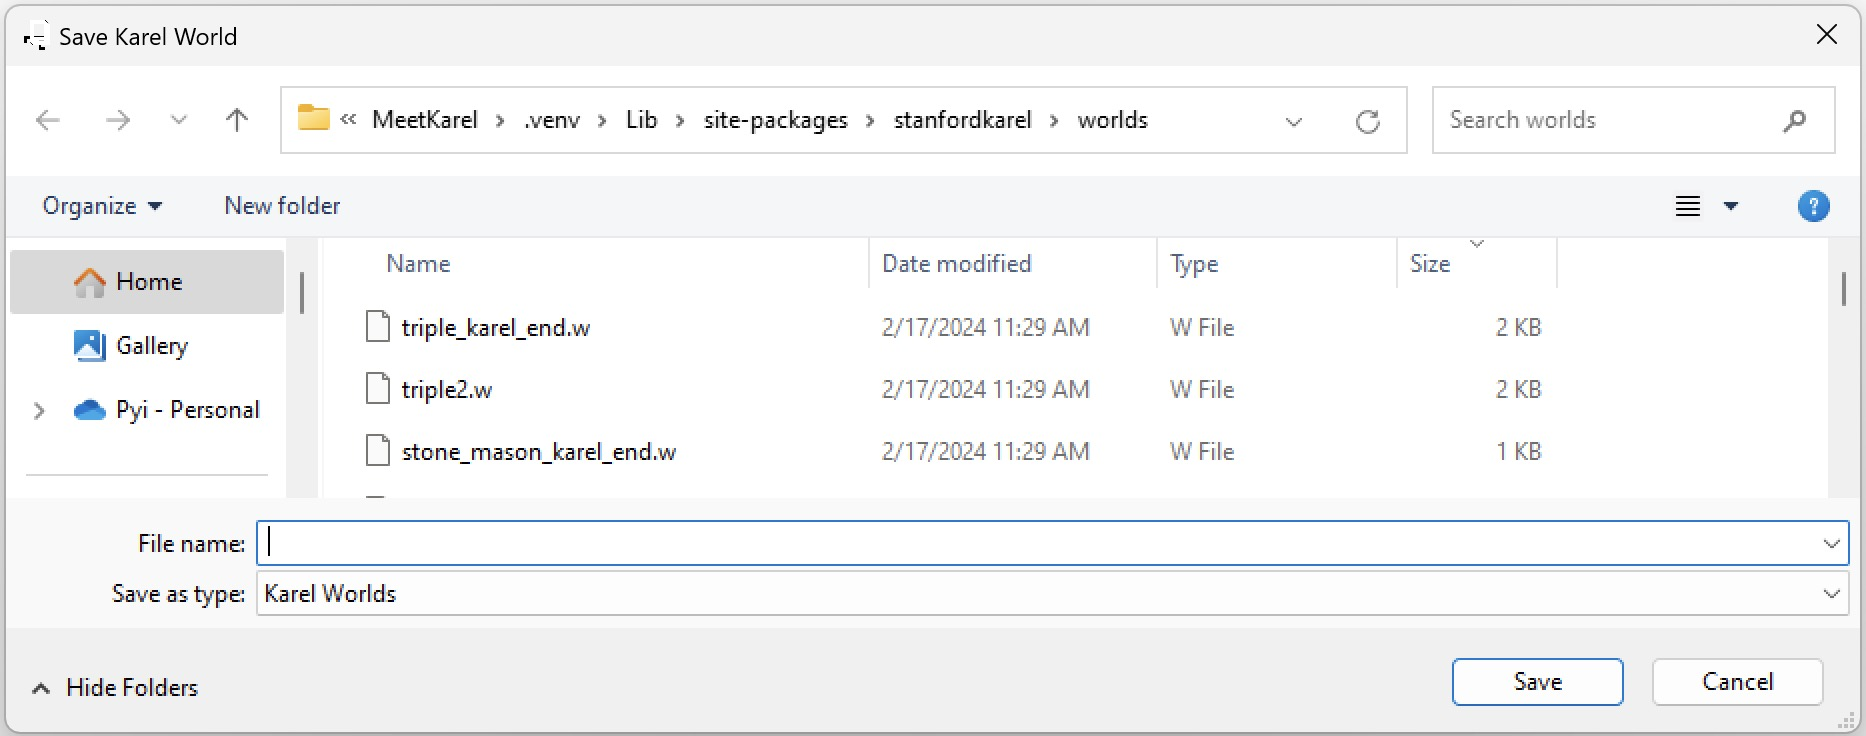
\includegraphics[width=.98\textwidth, trim={2.4mm 2cm 2mm 2mm},clip]{images/pycharm_install/default_worlds.jpg}};
    \drawshadow{image}
\end{tikzpicture}
\caption{} 
\label{fig:default_worlds}
\end{figure}

\begin{figure}[tbh!]
\begin{tikzpicture}
    \node[anchor=south west,inner sep=0] (image) at (0,0)
        {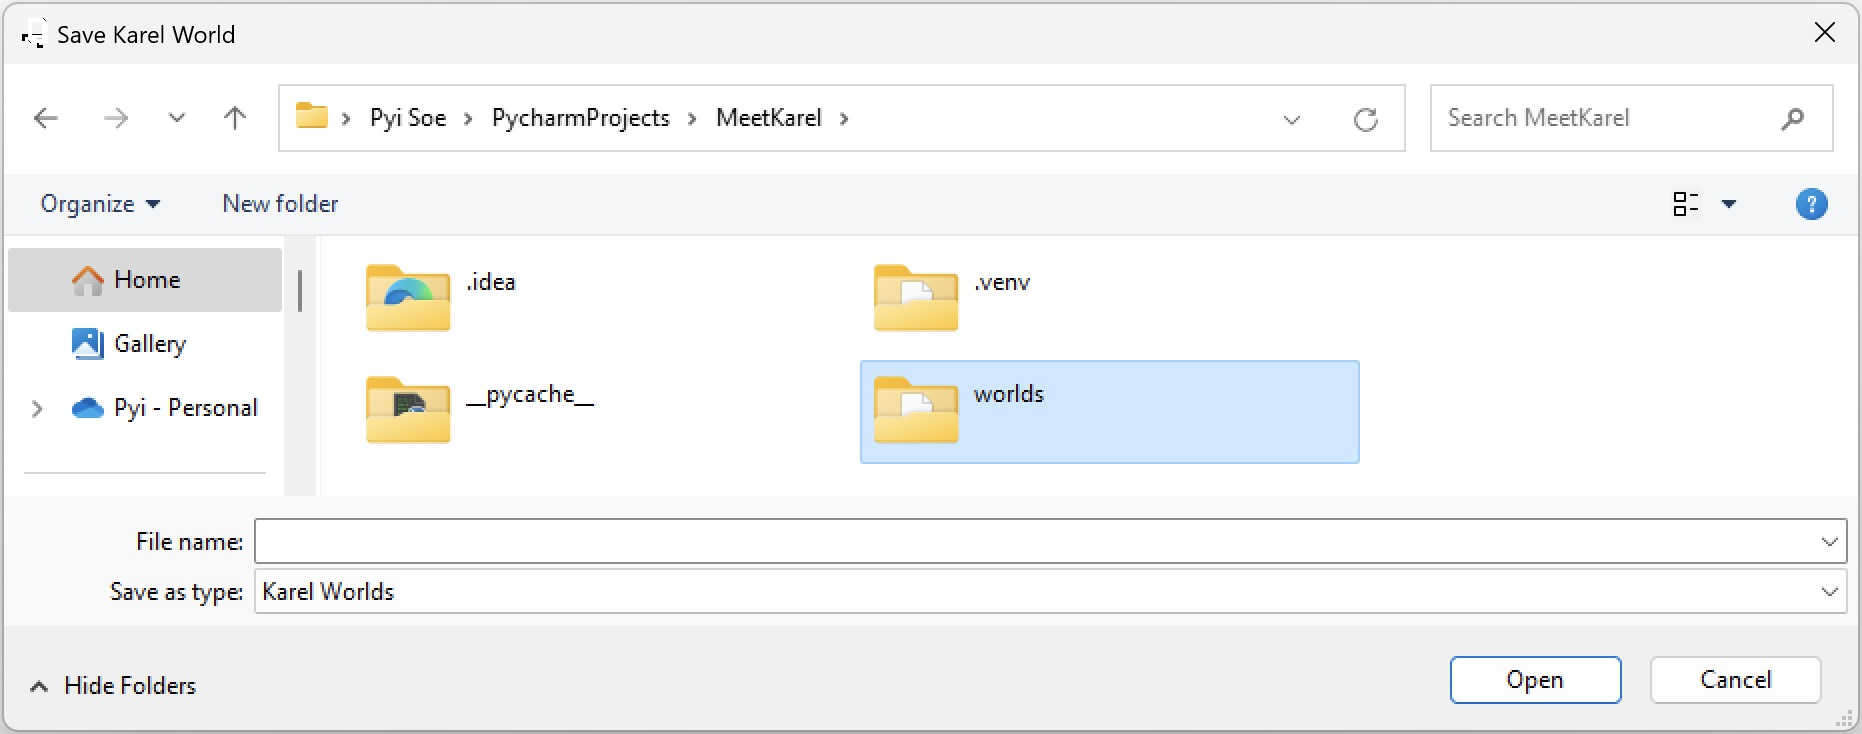
\includegraphics[width=.98\textwidth, trim={2.4mm 2cm 2mm 2mm},clip]{images/pycharm_install/proj_worlds.jpg}};
    \drawshadow{image}
\end{tikzpicture}
\caption{} 
\label{fig:proj_worlds}
\end{figure}


%\fEn{MeetKarel.zip} ကို \todo{ဒေါင်းလုဒ်လင့်ထည့်ရန်} ဒီ \fCode{https://tinyurl.com/yesz8a6j} လင့်ကနေ ဒေါင်းလုဒ်လုပ်၊ \fEn{extract} လုပ်ပြီး \fEn{lib, src, worlds} ဖိုဒါတို့ကို ပင်မ \fEn{project} ဖိုဒါအောက်မှာ ကော်ပီကူးထည့်ပါ။ \fEn{lib} ဖိုဒါကို \fEn{right click} နှိပ်ပြီး \fEn{Add as Library} လုပ်ပါ။ \fEn{src} ဖိုဒါထဲက \fEn{MeetKarel.java} ကိုဖွင့်ပြီး ပရိုဂရမ်ကို \fEn{run} ပါ။ ကားရဲလ် \fEn{Window} ပေါ်လာပါလိမ့်မယ်။ \fEn{Start Program} နှိပ်ရင် ကားရဲလ်က ဘိပါတုံးလေးကို နေရာရွှေ့ပေးပါလိမ့်မယ်။ (ပုံ \fRefNo{\ref{fig:proj_create01}} စာမျက်နှာ \fRefNo{\pageref{fig:proj_create01}} မှစ၍ \fRefNo{\ref{fig:proj_create13}} ထိ လိုအပ်ရင်ကြည့်ပါ)။ 

\clearpage


\afterpage{\blankpage}

\noindent \fEn{Python programming language}\\
\qquad \fCodeBf{import}\fEn{,} \fCodeBf{from}\fEn{,} \fCodeBf{def}\fEn{,} \fCodeBf{if}
\\
\noindent \fEn{New term}\\
\qquad \\fEnEmp{statement}


ပါရာမီတာမပါရင်လည်း ဝိုက်ကွင်းအလွတ် တစ်စုံ \fEn{‘\fCode{()}’} တော့ပါရမယ်။

\fEn{colon} \fEn{‘\fCode{:}’}

ဖန်ရှင်နဲ့ သက်ဆိုင်တဲ့ ကုဒ်ဘလောက် \fEn{(\textit{code block})}

\fEn{quote} သုံးခုတွဲ \fEn{‘\fCode{"""}’}

ပရိုဂရမ်ဝင်းဒိုးမှာ \mytcboxinl{\fEnSnd{Run Program}}  ခလုတ်

\mytcboxinl{\fEnSnd{meet\_karel.w}} ကမ္ဘာကို
\end{document}